
\documentclass[PhD]{uclathes}

%%<<140818>> update this preamble file in terms of the beamer version
%%<<141022>> merged the beamer version and the manu version together and re-locate it at latex_refs/
%%<<190330>> adapted for my thesis. Need to add the following line to bibtex. see: https://tex.stackexchange.com/questions/365215/natbib-newblock-undefined-error-with-informs3-document-class
\newcommand{\newblock}{}

%-------------- declare old font command, see
%               https://tex.stackexchange.com/questions/304311/is-there-any-reason-not-to-use-let-to-redefine-a-deprecated-control-sequence-to
\DeclareOldFontCommand{\rm}{\normalfont\rmfamily}{\mathrm}
\DeclareOldFontCommand{\sf}{\normalfont\sffamily}{\mathsf}
\DeclareOldFontCommand{\tt}{\normalfont\ttfamily}{\mathtt}
\DeclareOldFontCommand{\bf}{\normalfont\bfseries}{\mathbf}
\DeclareOldFontCommand{\it}{\normalfont\itshape}{\mathit}
\DeclareOldFontCommand{\sl}{\normalfont\slshape}{\@nomath\sl}
\DeclareOldFontCommand{\sc}{\normalfont\scshape}{\@nomath\sc}


\newcommand{\NimgTOT}{179}   %number of TOTal identified arc images
\newcommand{\NsysTOT}{57}   %number of TOTal identified arc systems
\newcommand{\NimgUSE}{72}   %number of USEd in model arc images
\newcommand{\NsysUSE}{25}   %number of USEd in model arc systems
\newcommand{\NimgELtot}{7}  %number of arc images showing emission lines with quality > 1
\newcommand{\NsysELtot}{5}   %number of arc systems showing emission lines with quality > 1
\newcommand{\NimgELhiQ}{5}   %number of arc images showing high-quality (3 or 4) emission lines  <=>  z_spec confirmed
\newcommand{\NsysELhiQ}{3}   %number of arc systems showing high-quality (3 or 4) emission lines  <=>  z_spec confirmed
\newcommand{\NELobjsQhi}{55}    %number of all the ELobjs with quality 3 or 4, including the \NimgELhiQ{} arcs
\newcommand{\NELQone}{2}        %number of singly lensed ELobjs with quality 1
\newcommand{\NELQtwo}{18}       %number of singly lensed ELobjs with quality 2
\newcommand{\NELQthree}{16}     %number of singly lensed ELobjs with quality 3
\newcommand{\NELQfour}{34}      %number of singly lensed ELobjs with quality 4


%%%%%%%%%%%%%%%%%%%%%%%%%%%%%%%%%%%%%%%%%%%%%%
%%%% packages and settings useful globally
%%%%%%%%%%%%%%%%%%%%%%%%%%%%%%%%%%%%%%%%%%%%%%
\usepackage[english]{babel} % default (American) English hyphenation
\usepackage[utf8]{inputenc} % useful to type directly diacritic characters
\usepackage[T1]{fontenc}    % Use vector fonts, so it zooms properly in on-screen viewing software
\usepackage{ae,aecompl}
\usepackage{graphicx}       % allows the usage of ``includegraphics''
\usepackage{natbib}         % enables the use of \citep and others; see http://merkel.zoneo.net/Latex/natbib.php
\usepackage{url}            % enables the use of url web links
\urlstyle{rm}
\usepackage{grffile}        % enables dots and underscores in .pdf filenames
\usepackage{mathtools}      % enables the use of various environments work, e.g., |align|, |dcases|, define symbols (see below), etc.
\usepackage{bbold}          % enables the use of \mathbb{1} as the identity matrix
\newcommand{\bb}{\mathbb}
\usepackage{bbm}            % enables the use of bold Greek symbols
\newcommand{\bs}{\boldsymbol}
%\DeclareGraphicsRule{.tif}{png}{.jpg}{.bmp}
\usepackage{multirow}       % enables the use of \multirow{num}{*}{text} in deluxetable
\usepackage{xspace}         % enables the use of \xspace in defining macros
%\usepackage{epstopdf}
\usepackage{ccaption}       % continuation of caption for figures containing multiple floats
\usepackage{amsmath,amssymb,amsxtra,amsfonts}   % to use pmatrix, etc.
\usepackage{txfonts}
\usepackage{deluxetable}
\usepackage{lscape}

%%%%%%%%%%%%%%%%%%%%%%%%%%%%%%%%%%%%%%%%%%%%%%
%%%% special packages and corresponding usages
%%%%%%%%%%%%%%%%%%%%%%%%%%%%%%%%%%%%%%%%%%%%%%
%-------------- provide circled numbers
%\usepackage{tikz}
%\newcommand*\circled[1]{\tikz[baseline=(char.base)]{\node[shape=circle,draw,inner sep=2pt] (char) {#1};}}
%-------------- use \mathsmaller and \mathlarger to resize math symbols
%\usepackage{relsize}
%-------------- for dynamic display of tables, see
%               http://www.math-linux.com/latex-26/article/how-to-make-a-presentation-with-latex-introduction-to-beamer
%\usepackage{colortbl}
%-------------- correct total number of pages for appendix, have to be commented off when using \appendix in ms.tex
%               http://texblog.org/2012/05/24/correct-total-number-of-pages-with-backup-slides-in-beamer-presentations/
%\usepackage{appendixnumberbeamer}
%-------------- strikethrough in beamer itemize, see
%               http://tex.stackexchange.com/questions/35767/in-beamer-how-to-strike-through-an-item-after-displaying
%\usepackage{ulem}       % turn \emph to \underline
%\renewcommand<>{\sout}[1]{\alt#2{\beameroriginal{\sout}{#1}}{#1}}
%-------------- enable the use of enumitem (e.g. for creating checkbox todo list, see below), see
%				http://tex.stackexchange.com/questions/24371/does-enumitem-conflict-with-beamer-for-lists
%\usepackage{enumitem}      %  NOTE: once uncommented, cannot use env {itemize, enumerate} any more
%\setitemize{label=\usebeamerfont*{itemize item}%
%  \usebeamercolor[fg]{itemize item}
%  \usebeamertemplate{itemize item}}
%%-------------- create checkbox and todo list in itemize (need to enable enumitem), see
%%               http://tex.stackexchange.com/questions/247681/how-to-create-checkbox-todo-list
%\usepackage{enumitem}      %  NOTE: once uncommented, cannot use env {itemize, enumerate} any more
%\newlist{todolist}{itemize}{2}
%\setlist[todolist]{label=$\square$}
%\usepackage{pifont}
%\usepackage{amsmath}
%\usepackage{amssymb}
%\newcommand{\cmark}{\ding{51}}%
%\newcommand{\xmark}{\ding{55}}%
%\newcommand{\done}{\rlap{$\square$}{\raisebox{2pt}{\large\hspace{1pt}\cmark}}%
%\hspace{-2.5pt}}
%\newcommand{\wontfix}{\rlap{$\square$}{\large\hspace{1pt}\xmark}}
%-------------- include videos, works for .flv, .mov format
%\usepackage{media9}
%-------------- encourage a break at this point
%\newcommand{\smallspace}{\vspace{3cm}\goodbreak}
%\newcommand{\bigspace}{\vspace{4.5cm}\goodbreak}
%\newcommand{\biggerspace}{\vspace{5.5cm}\goodbreak}
%-------------- put the points in the left margin, see latex_manuscripts/reference/hw3_sol_fin.tex
%\reversemarginpar
%\newcommand{\worth}[1]
%        {\mbox{}\marginpar{\em #1}\nolinebreak}%puts value in margin
%-------------- Flexible typesetting of table and figure floats, see: https://ctan.org/pkg/ctable
%\usepackage{ctable}
%-------------- add texts in box, see: https://tex.stackexchange.com/questions/36524/how-to-put-a-framed-box-around-text-math-environment/36528
%\usepackage{tcolorbox}
%-------------- define new column type, see: https://tex.stackexchange.com/questions/257128/how-does-the-newcolumntype-command-work
%\usepackage{array}
%\newcolumntype{L}[1]{>{\raggedright\let\newline\\\arraybackslash\hspace{5pt}}m{#1}}

% -----------------------------------------------------------------------------------------------
% Turning references and citations into hyperlinks in color
\usepackage{color}         % using color package; put color boxes around text: \fcolorbox{frame colour}{background colour}{text}
\definecolor{gold}{rgb}{1,0.80,0}
\definecolor{orange}{rgb}{1,0.5,0}
\definecolor{midgray}{gray}{0.3}
\definecolor{lblue}{rgb}{0,0.2,0.6}
\definecolor{dgreen}{rgb}{0.1,0.6,0.3}
\definecolor{purple}{rgb}{0.5019607843137255,0.0,0.5019607843137255}
\usepackage[colorlinks=true,citecolor=lblue,linkcolor=black]{hyperref}    % does not work when enabling draft, nor with beamer

% -----------------------------------------------------------------------------------------------
% Reference a section by ``section XX'', without generating text like ``subsection XX'' as is done by \autoref.
\newcommand{\secref}[1]{Section~\ref{#1}}
\newcommand{\figref}[1]{Figure~\ref{#1}}
\newcommand{\Eqref}[1]{Equation~(\ref{#1})}


%%%%%%%%%%%%%%%%%%%%%%%%%%%%%%%%%%%%%%%%%%%%%%
%%%% only necessary for poster
%%%%%%%%%%%%%%%%%%%%%%%%%%%%%%%%%%%%%%%%%%%%%%
%\usepackage{wrapfig}
%\usepackage{caption}

%%%%%%%%%%%%%%%%%%%%%%%%%%%%%%%%%%%%%%%%%%%%%%
%%%% only necessary for emulateapj
%%%%%%%%%%%%%%%%%%%%%%%%%%%%%%%%%%%%%%%%%%%%%%
% - - - - - - - - already defined
\newcommand\farcs{\mbox{$.\!^{\prime\prime}$}}    % arcsec with a decimal point in front
\newcommand\farcm{\mbox{$.\mkern-4mu^\prime$}}      % arcmin with a decimal point in front
\newcommand{\arcsec}{\mbox{$\!^{\prime\prime}$}\xspace}  % the unit of arcsec
\newcommand{\arcmin}{\mbox{$\!^{\prime}$}\xspace}          % the unit of arcmin
\newcommand{\arcdeg}{\mbox{$^{\circ}$}\xspace}             % the unit of arcdeg
% - - - - - - - - have to comment off when using emulateapj
\usepackage{marvosym}


%%%%%%%%%%%%%%%%%%%%%%%%%%%%%%%%%%%%%%%%%%%%%%
%%%% mathematical symbols
%%%%%%%%%%%%%%%%%%%%%%%%%%%%%%%%%%%%%%%%%%%%%%
%\font\fb=''[cmr10]'' %for use with \LaTeX command
% pre-existing symbols: \exp, \ln, \log
%\newcommand{\rmd}{\textrm{d}}
%\def\d{\textrm{d}}   % NOTE: \newcommad doesn't work but this works!
\def\prt{\partial}
\def\cP{{\cal P}}
\newcommand{\be}{\begin{equation}}
\newcommand{\ee}{\end{equation}}
\newcommand{\non}{\nonumber}
\newcommand{\ba}{\begin{align}}
\newcommand{\ea}{\end{align}}
\newcommand{\nt}{\notag}
\def\abs#1{\left|{#1}\right|}
\newcommand{\avg}[1]{\left<#1\right>}
%-------- provide define symbols
\newcommand{\defeq}{\vcentcolon=}
\newcommand{\eqdef}{=\vcentcolon}
%-------- formatted arrows
\newcommand{\Ra}{\ensuremath{\Rightarrow}\xspace}
\newcommand{\ra}{\ensuremath{\rightarrow}\xpace}
\newcommand{\lra}{\ensuremath{\Leftrightarrow}\xspace}
% Statistical mean (angle brackets)
\newcommand{\stmean}[1]{\langle{#1}\rangle}
\newcommand{\logg}{\log_{10}}	% base-10 logarithm
% Spatial-curvature function in cosmological distances.
\DeclareMathOperator{\sk}{S}
% Trace of a linear operator or matrix
\DeclareMathOperator{\tr}{tr}
% Differential (must be upright Roman letter, per MNRAS)
\DeclareMathOperator{\ud}{d}

%%%%%%%%%%%%%%%%%%%%%%%%%%%%%%%%%%%%%%%%%%%%%%
%%%% (astro)physical units and quantities
%%%%%%%%%%%%%%%%%%%%%%%%%%%%%%%%%%%%%%%%%%%%%%
% - - - - - - - - quantities
\newcommand{\Msun}{\ensuremath{M_\odot}\xspace}
\newcommand{\Rsun}{\ensuremath{R_\odot}\xspace}
\newcommand{\Lsun}{\ensuremath{L_\odot}\xspace}
\newcommand{\thE}{\ensuremath{\theta_{\rm E}}\xspace}
\newcommand{\chisq}{\ensuremath{\chi^2}\xspace}
\newcommand{\zspec}{\ensuremath{z_{\rm spec}}\xspace}
\newcommand{\zphot}{\ensuremath{z_{\rm phot}}\xspace}
\newcommand{\Mstar}{\ensuremath{M_\ast}\xspace}
\newcommand{\Lstar}{\ensuremath{L_\ast}\xspace}
\newcommand{\Sstar}{\ensuremath{\Sigma_\ast}\xspace}
\newcommand{\oh}{\ensuremath{12+\log({\rm O/H})}\xspace}
\newcommand{\Av}{\ensuremath{A_{\rm V}}\xspace}
\newcommand{\Rv}{\ensuremath{R_{\rm V}}\xspace}
\newcommand{\Te}{\ensuremath{T_{\rm e}}\xspace}
\def\ne{\ensuremath{n_{\rm e}}\xspace}
\newcommand{\SFR}{\ensuremath{{\rm SFR}}\xspace}
\newcommand{\Mgas}{\ensuremath{M_{\rm gas}}\xspace}
\newcommand{\Sgas}{\ensuremath{\Sigma_{\rm gas}}\xspace}
\newcommand{\fgas}{\ensuremath{f_{\rm gas}}\xspace}
\newcommand{\Zgas}{\ensuremath{Z_{\rm gas}}\xspace}
\newcommand{\tage}{\ensuremath{t_{\rm age}}\xspace}
\newcommand{\Vrot}{\ensuremath{V_{\rm rot}}\xspace}
\newcommand{\reff}{\ensuremath{r_{\rm eff}}\xspace}
\newcommand{\Dn}{\ensuremath{{\rm D}_n(4000)}\xspace}
\newcommand{\HdA}{\ensuremath{{\rm H}\delta_A}\xspace}
\newcommand{\scrit}{\ensuremath{\sigma_{\rm crit}}\xspace}

% - - - - - - - - units
\newcommand{\eV}{\ensuremath{\rm eV}\xspace}
\newcommand{\pc}{\ensuremath{\rm pc}\xspace}
\newcommand{\kpc}{\ensuremath{\rm kpc}\xspace}
\newcommand{\Mpc}{\ensuremath{\rm Mpc}\xspace}
\newcommand{\K}{\ensuremath{\rm K}\xspace}
\newcommand{\mK}{\ensuremath{\rm mK}\xspace}
\newcommand{\Hunit}{\ensuremath{\rm km~s^{-1}~Mpc^{-1}}\xspace}
\newcommand{\Funit}{\ensuremath{\rm erg~s^{-1}~cm^{-2}}\xspace}
\newcommand{\Flam}{\ensuremath{\rm erg~s^{-1}~cm^{-2}~\AA^{-1}}\xspace}
\newcommand{\Fnu}{\ensuremath{\rm erg~s^{-1}~cm^{-2}~Hz^{-1}}\xspace}
\newcommand{\muJy}{\ensuremath{\mu\rm Jy}\xspace}
\newcommand{\SBunit}{\ensuremath{\rm erg~s^{-1}~cm^{-2}~arcsec^{-2}}\xspace}
\newcommand{\magarcs}{\ensuremath{\rm mag~arcsec^{-2}}\xspace}
\newcommand{\Msunyr}{\ensuremath{\Msun~\mathrm{yr}^{-1}}\xspace}
\newcommand{\yr}{\ensuremath{\rm yr}\xspace}
\newcommand{\Myr}{\ensuremath{\rm Myr}\xspace}
\newcommand{\Gyr}{\ensuremath{\rm Gyr}\xspace}
\def\micron{\ensuremath{\mu\textrm{m}}\xspace}  % better than the default \micron, which does not use \xspace
\newcommand{\kms}{\ensuremath{\rm km~s^{-1}}\xspace}

%%%%%%%%%%%%%%%%%%%%%%%%%%%%%%%%%%%%%%%%%%%%%%
%%%% astrophysical aliases and jargons
%%%%%%%%%%%%%%%%%%%%%%%%%%%%%%%%%%%%%%%%%%%%%%
\newcommand\ionp[2]{#1$\;${\scshape{#2}}}      % ion permitted transitions, i.e., C IV = \ionp{C}{iv}
\newcommand\ionf[2]{[#1$\;${\scshape{#2}}]}    % ion forbidden transitions, i.e., [O III] = \ionf{O}{iii}
\newcommand\ions[2]{#1$\;${\scshape{#2}}]}     % ion semi-forbidden transitions, i.e., C III] = \ions{C}{iii}
\newcommand{\Ha}{\textrm{H}\ensuremath{\alpha}\xspace}
\newcommand{\Hb}{\textrm{H}\ensuremath{\beta}\xspace}
\newcommand{\Hg}{\textrm{H}\ensuremath{\gamma}\xspace}
\newcommand{\HII}{\textrm{H}\textsc{ii}\xspace}
\newcommand{\HI}{\textrm{H}\textsc{i}\xspace}
\newcommand{\Htwo}{\textrm{H}\ensuremath{_2}\xspace}
\newcommand{\He}{\textrm{He}\xspace}
\newcommand{\OI}{[\textrm{O}~\textsc{i}]\xspace}
\newcommand{\OII}{[\textrm{O}~\textsc{ii}]\xspace}
\newcommand{\OIII}{[\textrm{O}~\textsc{iii}]\xspace}
\newcommand{\CIII}{\textrm{C}~\textsc{iii}]\xspace}
\newcommand{\NII}{[\textrm{N}~\textsc{ii}]\xspace}
\newcommand{\SII}{[\textrm{S}~\textsc{ii}]\xspace}
\newcommand{\NeIII}{[\textrm{Ne}~\textsc{iii}]\xspace}
\newcommand{\sersic}{S\'{e}rsic\xspace}
\newcommand{\lya}{\textrm{Ly}\ensuremath{\alpha}\xspace}
% - - - - - - - - astrometric filters
\def\B{\ensuremath{B_{435}}\xspace}
\def\V{\ensuremath{V_{606}}\xspace}
\def\I{\ensuremath{I_{814}}\xspace}
\def\Y{\ensuremath{Y_{105}}\xspace}
\def\J{\ensuremath{J_{125}}\xspace}
\def\JH{\ensuremath{JH_{140}}\xspace}
\def\H{\ensuremath{H_{160}}\xspace}


%%%%%%%%%%%%%%%%%%%%%%%%%%%%%%%%%%%%%%%%%%%%%%
%%%% my specific macros for objects, software, instruments, telescopes, projects
%%%%%%%%%%%%%%%%%%%%%%%%%%%%%%%%%%%%%%%%%%%%%%
% - - - - - - - - celestial objects
\newcommand{\clyi}{MACS1149.6+2223\xspace}
\newcommand{\cler}{Abell 2744\xspace}
\newcommand{\clsan}{Abell 370\xspace}
\newcommand{\clsi}{MACS0416.1-2403\xspace}
\newcommand{\clwu}{MACS0717.5+3745\xspace}
\newcommand{\clliu}{RXJ2248.7-4431\xspace}
\newcommand{\clqi}{RXJ1347.5-1145\xspace}
\newcommand{\clba}{MACS0744.9+3927\xspace}
\newcommand{\cljiu}{MACS2129.4-0741\xspace}
\newcommand{\clshi}{MACS1423.8+2404\xspace}

% - - - - - - - - software
\newcommand{\pylf}{\textsc{pyLensFix}\xspace}
\newcommand{\lf}{\textsc{LensFix}\xspace}
\newcommand{\sw}{\textsc{SWunited}\xspace}
\newcommand{\sex}{\textsc{SExtractor}\xspace}
\newcommand{\emc}{\textsc{Emcee}\xspace}
\newcommand{\linmix}{\textsc{linmix}\xspace}
\newcommand{\adriz}{\textsc{AstroDrizzle}\xspace}
\newcommand{\dpac}{\textsc{DrizzlePac}\xspace}
\newcommand{\fast}{\textsc{FAST}\xspace}
\newcommand{\galfit}{\textsc{Galfit}\xspace}
\newcommand{\axe}{\textsc{aXe}\xspace}
\def\lt{\textsc{Lenstool}\xspace}
\newcommand{\glafic}{\textsc{Glafic}\xspace}
\newcommand{\gasoline}{\textsc{Gasoline}\xspace}
\newcommand{\ramses}{\textsc{Ramses}\xspace}
\newcommand{\SJ}{\textsc{Sharon \& Johnson}\xspace}
\newcommand{\grzl}{\textsc{Grzili}\xspace}
\newcommand{\burst}{\textsc{Starburst99}\xspace}

% - - - - - - - - projects, telescopes, instruments
\newcommand{\planck}{\textit{Planck}\xspace}
\newcommand{\hst}{\textit{HST}\xspace}
\newcommand{\jwst}{\textit{JWST}\xspace}
\newcommand{\spitzer}{\textit{Spitzer}\xspace}
\newcommand{\herschel}{\textit{Herschel}\xspace}
\newcommand{\chandra}{\textit{Chandra}\xspace}
\newcommand{\glass}{\textit{GLASS}\xspace}
\newcommand{\wisp}{\textit{WISP}\xspace}
\newcommand{\clash}{\textit{CLASH}\xspace}
\newcommand{\candels}{\textit{CANDELS}\xspace}
\newcommand{\hff}{\textit{HFF}\xspace}
\newcommand{\muse}{\textit{MUSE}\xspace}
\newcommand{\kmos}{\textit{KMOS}\xspace}
\newcommand{\keck}{\textit{Keck}\xspace}
\newcommand{\deimos}{\textit{DEIMOS}\xspace}
\newcommand{\mosfire}{\textit{MOSFIRE}\xspace}
\newcommand{\surfsup}{\textit{SURFSUP}\xspace}
\newcommand{\kd}{\textit{KMOS}$^{3\rm D}$\xspace}
\newcommand{\sdss}{\textit{SDSS}\xspace}
\def\clash{\textit{CLASH}\xspace}
\def\mosdef{\textit{MOSDEF}\xspace}
\newcommand{\vlt}{\textit{VLT}\xspace}
\newcommand{\osiris}{\textit{OSIRIS}\xspace}
\newcommand{\sinf}{\textit{SINFONI}\xspace}
\newcommand{\wfst}{\textit{WFIRST}\xspace}
\newcommand{\niriss}{\textit{NIRISS}\xspace}


%%%%%%%%%%%%%%%%%%%%%%%%%%%%%%%%%%%%%%%%%%%%%%
%%%% format, wording and abbreviations
%%%%%%%%%%%%%%%%%%%%%%%%%%%%%%%%%%%%%%%%%%%%%%
\def\etal{et al.\xspace}
\def\ie{i.e.\xspace}
\def\eg{e.g.\xspace}
\def\etc{etc.\xspace}
\def\aka{a.k.a.\xspace}
\def\vsv{vis-\'a-vis\xspace}
\renewcommand\({\left(}
\renewcommand\){\right)}
%\renewcommand\[{\left[}
%\renewcommand\]{\right]}

% - - - - - - - - word combo
\newcommand\mm{metallicity map\xspace}
\newcommand\mms{metallicity maps\xspace}
\newcommand\mg{metallicity gradient\xspace}
\newcommand\mgs{metallicity gradients\xspace}
\newcommand\Mgs{Metallicity gradients\xspace}
\newcommand\mgm{metallicity gradient measurement\xspace}
\newcommand\mgms{metallicity gradient measurements\xspace}
\newcommand\sr{spatially resolved\xspace}
\newcommand\srs{spatially resolved spectroscopy\xspace}
\newcommand\sra{spatially resolved analysis\xspace}
\newcommand\gp {gas-phase\xspace}
\newcommand\gpm{gas-phase metallicity\xspace}
\newcommand\subr{surface brightness\xspace}        % <<160715>> NOTE: cannot re-DEF \sb
\def\sf{star-forming\xspace}
\newcommand\sfr{star-formation rate\xspace}
\newcommand\sfh{star-formation history\xspace}
\newcommand\sfms{star-formation main sequence\xspace}

% - - - - - - - - specially formated words
\newcommand{\el}[1]{\ensuremath{\textrm{EL}_{#1}}}
\newcommand{\obs}{\textrm{o}}
\newcommand{\theo}{\textrm{t}}
\newcommand{\ext}{\textrm{ext}}
\def\det{\textrm{det}}
\newcommand\refe{\textrm{ref}}
\newcommand\pa{\textrm{PA}}

\def\p{{\rm prior}}
\def\fid{{\rm fid}}
\def\lnk{\kappa}
\def\lnkp{\kappa'}
%\newcommand{\n}{\noindent}


%%%%%%%%%%%%%%%%%%%%%%%%%%%%%%%%%%%%%%%%%%%%%%
%%%% lensing quantities and parameters
%%%%%%%%%%%%%%%%%%%%%%%%%%%%%%%%%%%%%%%%%%%%%%
\newcommand{\xa}{\alpha}
\newcommand{\xb}{\beta}
\newcommand{\xk}{\kappa}
\newcommand{\xg}{\gamma}
%\newcommand{\xg}[1]{|\gamma #1|}


%%%%%%%%%%%%%%%%%%%%%%%%%%%%%%%%%%%%%%%%%%%%%%
%%%% cosmological parameters
%%%%%%%%%%%%%%%%%%%%%%%%%%%%%%%%%%%%%%%%%%%%%%
\newcommand{\Or} {\ensuremath{\Omega_{\rm{r}}}\xspace}
\newcommand{\Om} {\ensuremath{\Omega_{\rm{m}}}\xspace}
\newcommand{\Ok} {\ensuremath{\Omega_{\rm{k}}}\xspace}
\newcommand{\Ol} {\ensuremath{\Omega_{\Lambda}}\xspace}
\newcommand{\Obh}{\ensuremath{\Omega_{\rm{b}}h^2}\xspace}
\newcommand{\Ob} {\ensuremath{\Omega_{\rm{b}}}\xspace}
\newcommand{\Onu}{\ensuremath{\Omega_\nu}\xspace}
\newcommand{\fnu}{\ensuremath{f_{\nu}}\xspace}
\newcommand{\Och}{\ensuremath{\Omega_{\rm{DM}}h^2}\xspace}
\newcommand{\Oc} {\ensuremath{\Omega_{\rm{DM}}}\xspace}
\newcommand{\ns} {\ensuremath{n_{\rm s}}\xspace}
\newcommand{\As} {\ensuremath{A_{\rm s}}\xspace}
%\newcommand{\nt} {\ensuremath{n_{\rm t}}\xspace}
%\newcommand{\At} {\ensuremath{A_{\rm t}}\xspace}
\newcommand{\thA}{\ensuremath{\theta_{\rm A}}\xspace}
%\newcommand{\run}{\ensuremath{{dn_s \over d\ln k}}\xspace}
\newcommand{\neff}{\ensuremath{N_\textrm{eff}}\xspace}
\newcommand{\mnu}{\ensuremath{\sum{m_{\nu}}}\xspace}
\newcommand{\yhe}{\ensuremath{Y_p}\xspace}
%\newcommand{\nrun}{\ensuremath{dn_s/d\ln k}\xspace}
\newcommand{\Map}[1]{\left<M^2_\textrm{ap}\right>( #1 )}
\newcommand{\map}{\ensuremath{\left<M^2_\textrm{ap}\right>}\xspace}
\newcommand{\chiH}{\ensuremath{\chi_\textrm{H}}\xspace}
\newcommand{\n}{\ensuremath{{\nu}\rm}\xspace}
\newcommand{\nue}{\ensuremath{{\nu}_{\rm e}}\xspace}
\newcommand{\num}{\ensuremath{{\nu}_{\rm \mu}}\xspace}
\newcommand{\nut}{\ensuremath{{\nu}_{\rm \tau}}\xspace}
\newcommand{\da}{\ensuremath{D_{\rm A}}\xspace}
\newcommand{\dl}{\ensuremath{D_{\rm L}}\xspace}
%\newcommand{\pripk}{\ensuremath{P_{\textrm{pri}}(k)}}
\newcommand{\taueq}{\ensuremath{\tau_{\rm eq}}\xspace}

%= = = = = = = = = = = = = = = = = = = = = = = = = = = = = = = = = = = = = = = =
% fancy header setup in P88
%\documentclass{book}
%\usepackage{fancyhdr}
%\pagestyle{fancy}
%% with this we ensure that the chapter and section
%% headings are in lowercase.
%\renewcommand{\chaptermark}[1]{%
%        \markboth{#1}{}}
%\renewcommand{\sectionmark}[1]{%
%        \markright{\thesection\ #1}}
%\fancyhf{}  % delete current header and footer
%\fancyhead[LE,RO]{\bfseries\thepage}
%\fancyhead[LO]{\bfseries\rightmark}
%\fancyhead[RE]{\bfseries\leftmark}
%\renewcommand{\headrulewidth}{0.5pt}
%\renewcommand{\footrulewidth}{0pt}
%\addtolength{\headheight}{0.5pt} % space for the rule
%\fancypagestyle{plain}{%
%   \fancyhead{} % get rid of headers on plain pages
%   \renewcommand{\headrulewidth}{0pt} % and the line
%}

                         % personal LaTeX macros
\input{ctx}
\input{journal_def}

%%%%%%%%%%%%%%%%%%%%%%%%%%%%%%%%%%%%%%%%%%%%%%%%%%%%%%%%%%%%%%%%%%%%%%
%
% Usually things live in separate flies.
%
% \input {prelim}                           % preliminary page info

%%%%%%%%%%%%%%%%%%%%%%%%%%%%%%%%%%%%%%%%%%%%%%%%%%%%%%%%%%%%%%%%%%%%%%%%
%                                                                      %
%                          PRELIMINARY PAGES                           %
%                                                                      %
%%%%%%%%%%%%%%%%%%%%%%%%%%%%%%%%%%%%%%%%%%%%%%%%%%%%%%%%%%%%%%%%%%%%%%%%

\title          {Dissecting the Baryon Cycle\\
                 at the Peak of Cosmic Star Formation\\
                 with Hubble Space Telescope Slitless Spectroscopy}
\author         {Xin Wang}
\department     {Astronomy and Astrophysics}
% Note:  degreeyear should be optional, but as of  5-Feb-96
% it seems required or you get a year of ``2''.   -johnh
\degreeyear     {2019}

%%%%%%%%%%%%%%%%%%%%%%%%%%%%%%%%%%%%%%%%%%%%%%%%%%%%%%%%%%%%%%%%%%%%%%%%

\chair          {Tommaso L. Treu}
\member         {Alice E. Shapley}
\member         {Matthew A. Malkan}
\member         {Omer M. Blaes}

%%%%%%%%%%%%%%%%%%%%%%%%%%%%%%%%%%%%%%%%%%%%%%%%%%%%%%%%%%%%%%%%%%%%%%%%

\dedication     {\textsl{To my wife Dr. Xiao-Lei Meng \\
                who have nourished and sustained me \\
                with her illuminating love \\
                especially during the darkest hours}}

%%%%%%%%%%%%%%%%%%%%%%%%%%%%%%%%%%%%%%%%%%%%%%%%%%%%%%%%%%%%%%%%%%%%%%%%

\acknowledgments{
First of all, I should thank my advisor Tommaso Treu, for his guidance, patience, and in particular his generous financial
support throughout the entire course of my PhD studies.
His ruthless pragmatism educated me of the urgency of publishing to avoid being replaced by collaborators.
I would also like to acknowledge my external advisor, Tucker Jones, who have helped me grow scientifically.
A significant portion of my PhD research is ``prototyped'' in his seminal work and I have been following his footsteps
ever since to have finally climbed over this monumental mountain called Doctor of Philosophy.

I am also greatly indebted to Louis Abramson. Tommaso and Tucker \emph{had} to deal with me, but for some reasons Louis \emph{chose} to.
His profound understanding of galaxy evolution combined with his eloquent arguments has always made our discussions highly
beneficial and enlightening to me.
An enormous thank you also goes to Takahiro Morishita.
He was my inspiration, as we face similar situations doing research abroad.
Being in a foreign country, where the speaking language does not resemble at all our mother tongues,
we can only earn respect through hard work, wholehearted dedication, and unique expertise.
In a way, Takahiro showed me a path and I am so proud that I have found the courage to follow it.

I would never take for granted the ample opportunities of close collaborations with experts in the field, who have
helped transform me into a confident and resourceful astronomer.
First and foremost, I would say millions of thank you to Gabe Brammer, for giving me the precious chance to come to STScI to
receive face-to-face hands-on training on grism data reduction from him, and answering me numerous questions on
astronomical data analysis in general.  ``Learning from Achilles himself; kings would kill for the honor.'' I am
sincerely grateful for having the great opportunity to collaborate with and learn from Emanuele Daddi.  He played
a crucial role in helping develop the inverted gradient discovery paper, and really expanded my horizon on the
physics of galaxy evolution. I cannot thank Keren Sharon enough for her help and advice, as well as giving me the
awesome chance to visit UMich.  She is the one who redeemed my faith in gravitational lensing
for galaxy clusters, by teaching me Lenstool step-by-step, which now has become an indispensible part in my skill
set.  Matt Malkan is greatly appreciated for his pivotal help in securing a postdoc position for me at
Caltech/IPAC starting this summer, and for allowing me to join the WISPs collaboration.  I acknowledge Kasper
Schmidt and Kuang-Han Huang, who initiated me on Python programming.

I would also like to thank Omer Blaes, Matt Malkan, Alice Shapley and Tommaso Treu for serving on my dissertation
committee.

My deep gratitude also goes to all my fellow graduate students at both UCSB and UCLA, in particular, Suoqing Ji,
Xinnan Du, and Ryan Sanders.
Suoqing started graduate school at UCSB in the same year as I did, and has given me some great tips in
transitioning to US life.
Becoming close friends with Suoqing is one of the few things that made my days at UCSB not a total failure.
Xinnan helped me a great deal with my transfer from UCSB to UCLA.
Without her invaluable help, I could not have won the prestigious Chinese Government Award for Outstanding
Graduate Student Abroad.
Ryan served as my graduate student mentor for over a year, and set up an excellent role model for me.
I sincerely thank him for proof-reading my proposals/papers numerous times.
Also acknowledged are the Treu group members whom I have been sharing pizzas with:
Alessandro Sonnenfeld, Simon Birrer, Peter Williams, Anowar Shajib, Daniel Gilman, Xuheng Ding, Lilan Yang.

I would also like to appreciate the kindness and assistance from local people when I visited their institutes.
First of all, Prof. Shude Mao is wholeheartedly acknowledged for giving me multiple opportunities of lengthy visits to THCA.
Bravo on the recently founded Department of Astronomy.
I am also truly grateful to the help and financial support from Prof. Le Zhang for my visit to SJTU, 
Prof. Xu Kong for my visit to USTC, Prof. Yu Gao for my visit to PMO, Prof. Gongbo Zhao for my visit to NAOC.
Furthermore, thank you also goes to Jessie Hirtenstein at UC Davis,
Raymond Simons, Alaina Henry and Ivelina Momcheva at STScI,
Yuan-Sen Ting at IAS,
Jacqueline van Gorkom at Columbia,
Xiangcheng Ma, Phil Hopkins, Nicha Leethochawalit and Evan Kirby at Caltech,
Xiangcheng Ma (again), Yuan Li, and Dan Weisz at UC Berkeley,
Zheng Cai, Joseph Burchett and Song Huang at UCSC.
Since my college day one, I have been living in the giant shadow shaded by Song; 
his fanatic passion for astronomy is extremely contagious and has always spurred me onto greater effort in
pursuit of astronomical achievements.
My special gratitude to Hui Li, whos is also a Nanjing University alumnus.
He provided tremendous help to me when I visited Ann Arbor as well as Boston.
Congratulations to his recent achievement on the Hubble fellowship.
Last but not the least, the professors at Nanjing University, i.e., Profs. Zhiyuan Li, Yong Shi, Qiu-Sheng Gu,
Yong Feng Huang, Jilin Zhou, etc., are cordially acknowledged for my several trips back to my Alma Mater.
It is always a mind-blowing pleasure to see that Astronomy at NJU has expanded on such a large scale in recent
years and I look forward to its everlasting growth.

Last but not the least, without my parents, I could not have been here in the first place. Their care and
support, both financially and emotionally, are the cornerstones of every piece of my achievements, ever since I
was a little kid.
My last and best spot is always reserved for the love of my life, Xiaolei!
But nothing written down could come even close to do justice to your love and what it means to me.
Earning a PhD is a tumultuous and hectic journey.
Without you, I would have long been lost.

}

%%%%%%%%%%%%%%%%%%%%%%%%%%%%%%%%%%%%%%%%%%%%%%%%%%%%%%%%%%%%%%%%%%%%%%%%

\vitaitem{2006}{Graduated, Yaohua High School, Tianjin, China}
\vitaitem{2010}{Bachelor of Science in Astronomy, Summa Cum Laude, Department of Astronomy, Nanjing University, Jiangsu Province, China}
\vitaitem{2013}{Master of Science in Astrophysics, School of Astronomy and Space Sciences, Nanjing University, Jiangsu Province, China}
\vitaitem{2015}{Master of Arts in Physics, Physics Department, University of California, Santa Barbara, California, USA}
\vitaitem{2018}{Dissertation Year Fellowship, University of California, Los Angeles, California, USA}

%%%%%%%%%%%%%%%%%%%%%%%%%%%%%%%%%%%%%%%%%%%%%%%%%%%%%%%%%%%%%%%%%%%%%%%%

\publication{\input{include/publications}}

%%%%%%%%%%%%%%%%%%%%%%%%%%%%%%%%%%%%%%%%%%%%%%%%%%%%%%%%%%%%%%%%%%%%%%%%

\abstract{To explore the chemo-structural properties of galaxies and understand quantitatively the cycling of baryons at
the peak epoch of cosmic star formation, I developed a highly effective method for sub-kiloparsec scale spatially
resolved spectroscopy of strongly lensed galaxies using space-based wide-field slitless grism data.  Applying
this method to the deep Hubble Space Telescope (HST) near-infrared grism observations, I obtained precise
gas-phase metallicity maps for a large sample of star-forming galaxies in the redshift range of $1.2\lesssim
z\lesssim2.3$. Over
half of the galaxies in my sample reside in the dwarf mass regime ($\Mstar\lesssim10^9 \Msun$), making my sample the first
statistically representative sample of high-redshift dwarf galaxies with their metallicity spatial distribution
measured with sufficient resolution.  The metallicity maps obtained in my work reveal a variety of baryonic
physics, such as efficient radial mixing from tidal torques, rapid accretion of low-metallicity gas, and various
feedback processes which can significantly influence the chemo-structural properties of star-forming galaxies.
For the first time, I discovered two dwarf galaxies at $z\sim2$ displaying strongly inverted metallicity radial
gradients, suggesting that powerful galactic winds triggered by central starbursts carry the bulk of stellar
nucleosynthesis yields to the outskirts.  I also observed an intriguing correlation between stellar mass and
metallicity gradient, consistent with the ``downsizing'' galaxy formation picture that more massive galaxies are
more evolved into later phases of disk growth, where they experience more coherent mass assembly at all radii
and thus show shallower metallicity gradients.  Furthermore, 10\% of the metallicity gradients measured in my
sample are inverted, which are hard to explain by currently existing hydrodynamical simulations and analytical
chemical evolution models.  My method can be readily applied to data from future space missions employing grism
instruments, e.g., JWST, Euclid, WFIRST.  Combined with the continuous input of HST resources, these data will
revolutionize our understanding of the chemo-structural evolution of galaxies throughout vast cosmic time.
}

%%%%%%%%%%%%%%%%%%%%%%%%%%%%%%%%%%%%%%%%%%%%%%%%%%%%%%%%%%%%%%%%%%%%%%%%


\begin{document}
\makeintropages

%%%%%%%%%%%%%%%%%%%%%%%%%%%%%%%%%%%%%%%%%%%%%%%%%%%%%%%%%%%%%%%%%%%%%%
% Ordinarily each chapter (at least) is in a separate file.
%

\chapter{Introduction}

\section{What is the baryon cycle and why is it important?}

Baryon cycle is the cycling of the cosmic baryon budget through star formation and gas flows. Galaxies grow by
getting their fuel from the intergalactic medium (gas inflows), converting it into stars (star formation), and
returning energy/material to their surroundings (gas outflows). Figure~\ref{fig:M82} presents a vivid example of
this complex phenomenon in the local Universe.
%= = = = = = = = = = = = = = = = = = = = = = = = = = = = = = = = = = = = = = = =
%%% Figures: M82
\begin{figure}
    \centering
    \includegraphics[width=0.8\textwidth]{/Users/albert/Dropbox/latex_figures/schematics/M82_gasflows_texted.png}
    \caption[Onset of baryon cycling in the local Universe: M82.]{Onset of baryon cycling in the local Universe: the Messier 82
    galaxy. Overlaid are the conjectured movements of gas in and around this galaxy undergoing active star
    formation.
    \label{fig:M82}}
\end{figure}
%- - - - - - - - - - - - - - - - - - - - - - - - - - - - - - - - - - - - - - - -
While we have developed a concordance cosmological framework of the $\Lambda$ cold dark matter ($\Lambda$CDM)
hierarchical structure formation \citep[see \eg][and references therein]{PlanckCollaboration:2018va}, 
we still lack a quantitative and coherent understanding of these baryonic
processes, without which the formation and evolution of galaxies, e.g., our Milky Way (MW), cannot be
characterized in detail.

\section{How can we observe the baryon cycle at the peak of cosmic star formation?}

The integral field spectroscopy (IFS) has expanded our vision of galaxies from integrated spectroscopic
quantities extracted from small subregions through single slits/fibres to panoramic 2-dimensional (2D) views
across their full surfaces, allowing for spatial variations of physical properties.  This facilitates several
large ground-based surveys, \eg, MaGNA \citep{Bundy:2015ft,Law:2015hc}, SAMI
\citep{TheSAMIGalaxySurv:wpN2l47X,Medling:2018hx}, CALIFA \citep{Sanchez:2016cs}, to capture the dynamic
signatures of the baryon cycle in action.
%rich baryonic processes of galaxy assembly, feedback, and chemical enrichment in fine spatial richness.
Yet the requirement of sufficient sampling, \ie, on sub-kiloparsec (sub-kpc) scale, to accurately map interesting
kinematic features and spatial structures have limited the focus of such surveys to nearby galaxies
($z\lesssim0.03$).  However, the local Universe is only the downhill of cosmic star formation, and the true
climax of baryonic mass assembly and chemical enrichment happens at the epoch of $1\lesssim z\lesssim3$, as shown
in Figure~\ref{fig:cosmic_noon} \citep[see \eg, ][and references there in]{2014ARA&A..52..415M,Abramson:2016wf}.
%= = = = = = = = = = = = = = = = = = = = = = = = = = = = = = = = = = = = = = = =
%%% Figures
\begin{figure}
    \centering
    \includegraphics[width=.8\textwidth]{/Users/albert/Dropbox/latex_figures/othersPaper/abramson16_fig1_noon.png}
    \caption[The rise and fall of the cosmic average star-formation rate density.]{The rise and fall of the
    cosmic average star-formation rate density.
    The grey shaded region marks the peak epoch of cosmic star formation, usually coined the ``cosmic noon''.
    At the cosmic noon, our Universe assembled roughly one half of its present day stellar mass using less than one third of its age.
    Figure credit: \citet{Abramson:2016wf}.
    \label{fig:cosmic_noon}}
\end{figure}
%- - - - - - - - - - - - - - - - - - - - - - - - - - - - - - - - - - - - - - - -

Numerical hydrodynamic simulations are by design capable of reproducing realistic galaxies at this epoch, by
modeling various baryonic processes as sub-grid prescriptions
\citep{Dave:2017gd,FIRESimulations:2017wj,Pillepich:2019uz}. The vast majority of observational programs
targetting cosmic-noon galaxies only measure their integrated spectroscopic quantities through single slits.
Albeit offering great insight on the physics of galaxy formation and evolution at a population level, this kind
of integrated spectroscopy lacks the ability to dissect the baryon cycle in individual systems.
%However, there is ample evidence that the morphological transformation also occurs during the cosmic noon
%\citep{Mortlock:2013dg}, such that the predominant shape of galaxies change from irregular to ordered structure,
%\ie, disk and bulge, which have drastically different spectral properties. Neglecting this distinction might
%result in a biased picture of the baryon cycle.  In Fig.~\ref{fig:ers}, I demonstrate such bias associated with
%the derivation of key physical properties from spectroscopy with partial spatial coverage.
Ground-based IFS is no longer capable of probing the necessarily fine details at sub-kpc scale, ascribed to the
atmospheric beam smearing effect and the intrinsically small size of high-$z$ galaxies.  As displayed in
Figure~\ref{fig:spatial_resolution}, the half-light radius of a typical \Lstar galaxy at $z$$\sim$2 is
$\sim$2.5\kpc. In comparison, the optimal median seeing of $\sim$$0\farcs6$ is equivalent to a physical size of
$\sim$5\kpc, resulting in the vast majority of $z$$\sim$2 star-forming galaxies unresolved.  The assistance of
adaptive optics (AO) can mitigate this problem, yet is challenging due to several reasons: low Strehl ratio and
throughput, dearth of tip/tilt stars, narrow field of view with limited multiplexing capability, etc.  Therefore,
we need a more effective approach for sub-kpc scale spatially resolved spectroscopy of cosmic noon sources to
compare statistically with theoretical results of cosmological zoom-in simulations, to shed light upon the
cycling of baryons.

%= = = = = = = = = = = = = = = = = = = = = = = = = = = = = = = = = = = = = = = =
%%% Figures
\begin{figure}
    \centering
    \includegraphics[width=0.8\textwidth]{/Users/albert/Dropbox/latex_figures/schematics/spatial_resolution_difference.png}
    \caption[The relationship among the effective radius, star-formation rate and stellar mass for galaxies at
    $z\sim2$.]{The relationship among the effective radius, star-formation rate and stellar mass for galaxies at $z\sim2$ covered by the CANDELS survey.
    The region where MW progenitors reside according to abundance matching is denoted by a red circle.
    The spatial resolution from natural seeing, native HST, and with gravitational lensing magnification combined
    are marked by the horizontal lines.
    We see that the only feasible approach to unambiguously resolve the MW progenitors is through the synergy of HST
    diffraction limit and lensing magnification.
    Figure credit: \citet{Wuyts:2012iw}.
    \label{fig:spatial_resolution}}
\end{figure}
%- - - - - - - - - - - - - - - - - - - - - - - - - - - - - - - - - - - - - - - -

%= = = = = = = = = = = = = = = = = = = = = = = = = = = = = = = = = = = = = = = = paragraph about GLASS and
%slitless grism spectroscopy from HST
In my dissertation, I took a different route.  The native resolution of the wide-field camera three (WFC3)
onboard the Hubble Space Telescope (\hst) is $\sim0\farcs13$, equivalent to a spatial scale of $\sim$1\kpc at
$z\sim2$ (cf.  Figure~\ref{fig:spatial_resolution}), already matching the spatial resolution achieved by the
aforementioned IFS surveys (\ie MaGNA, SAMI, CALIFA) in mapping the physical properties of nearby galaxies.  This
spatial sampling rate is unhampered by atmospheric turbulence because the telescope is floating on top.  The
infrared (IR) spectroscopy on HST is enabled by the WFC3 grism elements.  During observation, light from the
science target is dispersed along a certain spatial axis pertinent to the telescope's roll angle \emph{without
any slits}.  As a consequence, source morphology along the light dispersion direction is convolved onto the
wavelength axis, causing the morphological broadening effect \citep{vanDokkum:2011cq}.  As shown in
Figure~\ref{fig:macs1149_grism}, using some state-of-the-art data reduction techniques, I have been able to
extract the appropriate 2D spectral information of my targets in spite of the heavy blending of neighboring
objects and morphological broadening effect, to facilitate subsequent spatially resolved analysis.

The gravitational lensing phenomenon further improves the spatial resolution by roughly $\sqrt{\mu}$,
where $\mu$ is the lensing magnification factor.
Thus by targeting cosmic-noon galaxies in the background and
gravitationally lensed by foreground clusters of galaxies with the \hst WFC3/IR grism elements, I exploit the
lensing boost of \hst's resolving power to achieve sub-kpc scale spatial sampling of high-$z$ galaxies.
Therefore I compile a statistically significant sample of star-forming galaxies at cosmic noon,
whose spatial distribution of key physical properties are mapped out \emph{precisely}.
These properties include stellar mass (\Mstar), star-formation rate (SFR), gas-phase
metallicity\footnote{Throughout this dissertation I refer to the relative abundance of oxygen to hydrogen in the
interstellar medium as gas-phase metallicity, or just metallicity for simplicity.}, dust extinction, stellar
population age, total gas mass, etc.
This sample of galaxies has been shown to provide key insights into the effects of gas flows and feedback on the
cycling of baryons at the cosmic noon.

%= = = = = = = = = = = = = = = = = = = = = = = = = = = = = = = = = = = = = = = =
%%% Figures
\begin{figure}
    \centering
    \includegraphics[width=\textwidth]{/Users/albert/Dropbox/latex_figures/grismReduction/M1149_PA111_grismdemo.png}
    \caption[State-of-the-art data reduction techniques for \hst WFC3/IR slitless spectroscopy.]{
    State-of-the-art data reduction techniques for \hst WFC3/IR slitless spectroscopy are developed and adopted 
    throughout my dissertation work.
    \textit{Left}: the color-composite image of the galaxy cluster \clyi, where the first multiply imaged
    supernova (\ie SN Refsdal) is discovered, as marked by the white arrows \citep{2015Sci...347.1123K}.
    \textit{Middle}: the discovery of SN Refsdal triggers an HST follow-up grism program (Proposal ID 14041, P.I.
    Kelly) exposing the center of \clyi with 30 orbits of WFC3/G141 split equally into 2 position angles.
    The obtained grism exposure from one of them is shown here.
    The analysis of these data constitutes a significant part in my dissertation work (see Chapter 3).
    \textit{Right}: Due to the slitless nature of \hst grism spectroscopy, severe blending takes place for
    neighboring objects along the light dispersion direction (see the middle panel).
    The data reduction techniques used throughout my dissertation work (see Chapter 4 for more details) 
    properly account for this neighbour contamination and construct 2D spectral models for all sources 
    within the WFC3 field of view (FoV).
    These spectral models are refined iteratively until a convergence point where the residual in the grism
    exposures after subtracting the fitted continuum models becomes negligible, which is shown here.
    Figure credit: Gabe Brammer.
    \label{fig:macs1149_grism}}
\end{figure}
%- - - - - - - - - - - - - - - - - - - - - - - - - - - - - - - - - - - - - - - -


%= = = = = = = = = = = = = = = = = = = = = = = = = = = = = = = = = = = = = = = =
\section{Dissertation Overview}

The content of my dissertation is briefly described as follows.

Chapter 2 is adapted from my first-author paper published as Wang et al. (2015), ApJ, 811, 29, DOI:
10.1088/0004-637X/811/1/29, and is reproduced with permission from the AAS.
It presents a strong and weak lensing reconstruction of the massive cluster \cler, the first cluster for
which deep Hubble Frontier Fields (\hff) images and spectroscopy from the Grism Lens-Amplified Survey from Space
(\glass) are available.
By performing a targeted search for emission lines in multiply imaged sources using the
GLASS spectra, I obtain five high-confidence spectroscopic redshifts and two tentative ones. I confirm one
strongly lensed system by detecting the same emission lines in all three multiple images. I also search for
additional line emitters blindly and use the full GLASS spectroscopic catalog to test reliability of photometric
redshifts for faint line emitters. I see a reasonable agreement between our photometric and spectroscopic
redshift measurements, when including nebular emission in photometric redshift estimations. I introduce a
stringent procedure to identify only secure multiple image sets based on colors, morphology, and spectroscopy. By
combining 7 multiple image systems with secure spectroscopic redshifts (at 5 distinct redshift planes) with 18
multiple image systems with secure photometric redshifts, I reconstruct the gravitational potential of the
cluster pixellated on an adaptive grid, using a total of 72 images. The resulting mass map is compared with a
stellar mass map obtained from the deep \spitzer Frontier Fields data to study the relative distribution of stars
and dark matter in the cluster. I find that the stellar to total mass ratio varies substantially across the
cluster field, suggesting that stars do not trace exactly the total mass in this interacting system. 

Chapter 3 is adapted from my first-author paper published as Wang et al. (2017), ApJ, 837, 89, DOI:
10.3847/1538-4357/aa603c, and is reproduced with permission from the AAS.
I combine the deep \hst grism spectroscopy from both \glass and the SN Refsdal follow-up program (see
Figure~\ref{fig:macs1149_grism}) with a new Bayesian method to derive maps of gas-phase
metallicity for 10 star-forming galaxies at
high redshift ($1.2\lesssim z \lesssim2.3$). Exploiting lensing magnification by the foreground cluster \clyi, I
reach sub-kpc spatial resolution and push the limit of stellar mass associated with such high-z spatially
resolved measurements below $10^8$ \Msun for the first time. My maps exhibit diverse morphologies, indicative of
various effects such as efficient radial mixing from tidal torques, rapid accretion of low-metallicity gas, and
other physical processes that can affect the gas and metallicity distributions in individual galaxies. Based upon
an exhaustive sample of all existing sub-kpc resolution metallicity gradient measurements at high $z$, I find
that predictions given by analytical chemical evolution models assuming a relatively extended star-formation
profile in the early disk-formation phase can explain the majority of observed metallicity gradients, without
involving galactic feedback or radial outflows.  I observe a tentative correlation between stellar mass and
metallicity gradients, consistent with the ``downsizing'' galaxy formation picture that more massive galaxies are
more evolved into a later phase of disk growth, where they experience more coherent mass assembly at all radii
and thus show shallower metallicity gradients. In addition to the spatially resolved analysis, I compile a sample
of homogeneously cross-calibrated integrated metallicity measurements spanning three orders of magnitude in
stellar mass at $z\sim1.8$. We use this sample to study the mass-metallicity relation (MZR) and find that the
slope of the observed MZR can rule out the momentum-driven wind model at a 3-$\sigma$ confidence level.

Chapter 4 is adapted from my first-author paper currently under review, \ie, Wang et al. (2018), arXiv:1808.08800.
I report the first sub-kpc spatial resolution measurements of strongly inverted gas-phase 
metallicity gradients in two dwarf galaxies at $z$$\sim$2.
The galaxies have stellar masses $\sim$$10^9$\Msun, specific star-formation rate $\sim$20 \Gyr$^{-1}$, and 
global metallicity $\oh\sim8.1$ (1/4 solar).
Their metallicity radial gradients are measured to be highly inverted, \ie, 0.122$\pm$0.008 and 
0.111$\pm$0.017 dex/kpc, which is hitherto unseen at such small masses in similar redshift ranges.
From the HST observations of the source nebular emission and stellar continuum, I
present the 2D spatial maps of star-formation rate surface density, stellar population age, and 
gas fraction, which show that the two galaxies are currently undergoing rapid mass assembly via disk 
inside-out growth.  More importantly, using a simple chemical evolution model, I find that the gas 
fractions for different metallicity regions cannot be explained by pure gas accretion.  My spatially 
resolved analysis based on a more advanced gas regulator model results in a spatial map of net gaseous 
outflows, triggered by active central starbursts, that potentially play a significant role in shaping the 
spatial distribution of metallicity by effectively transporting stellar nucleosynthesis yields outwards.  
The relation between wind mass loading factors and stellar surface densities measured in different regions 
of our galaxies shows that a single type of wind mechanism, driven by either energy or momentum 
conservation, cannot explain the entire galaxy.  These sources present a unique constraint on the effects 
of gas flows on the early phase of disk growth from the perspective of spatially resolved chemical 
evolution within individual systems.

Chapter 5 is a summary of my previous work and concludes with a prospect of my ongoing analyses.




\chapter{Mass Reconstruction of the Lensing Cluster Abell 2744 from \protect\hff Imaging and \protect\glass Spectroscopy}


\section{Introduction}
\label{sec:intro}

In the past two decades, gravitational lensing by clusters of galaxies has transitioned from an exotic curiosity to an invaluable 
tool for astrophysics and cosmology \cite[e.g.][]{K+N11}. Clusters can act as natural telescopes, magnifying background sources so 
that they appear brighter and more extended to the observer \cite[e.g.][]{Yee++96,Pet++02,Shi++14,Bay++14}.  The 
gravitational lensing effect can also be used to reconstruct the spatial distribution of mass in the clusters themselves, thus 
shedding light on the physics of dark matter and structure formation 
\citep[e.g.][]{clowe06,Bra++06,San++08,New++13,Sha++14,2015ApJ...806....4M}.

In the past two years, clusters of galaxies as tools for cosmology and
astrophysics have become a major focus of a \hubble Space Telescope
(\hst) initiative. As part of the \hubble Frontier Field (HFF) program\footnote{\url{http://www.stsci.edu/hst/campaigns/frontier-fields/FF-Data}},
six clusters of galaxies and six parallel fields are being imaged to
unprecedented depths in seven optical and near-infrared (NIR) bands, using
the Wide Field Camera 3 (WFC3) and the Advanced Camera for Surveys
(ACS) \citep{2015ApJ...800...84C}. Similarly to previous public campaigns in
legacy fields such as the \hubble Deep Fields
\citep{Wil++96,Ferguson:2000p22537}, this major \hst campaign has
triggered coordinated observations with all major facilities, ranging
from Director's Discretionary time on the \spitzer Space Telescope to
deep observations with the Chandra X-ray Telescope and many ground
based facilities.

One of the major drivers of the HFF initiative is to search for
magnified objects behind galaxy clusters. Accurate magnification maps
are needed to determine the unlensed (intrinsic) properties of these
galaxies. Fortunately, the deep images increase significantly the
number of known multiply imaged systems per cluster, thus improving
dramatically the fidelity of the mass models, and magnification
maps. Typical CLASH\footnote{\url{http://www.stsci.edu/~postman/CLASH/Home.html}}-like depth imaging of clusters
\citep[limiting magnitude $\sim$ 27 ABmag for a 5-$\sigma$ point
source][]{Postman:2012p27556} yields a handful of multiple image
systems per cluster \cite[e.g.][]{Joh++14}, however at the depth of the HFF
we expected to find tens of multiply image systems. This was
beautifully confirmed by the first papers that analyzed the HFF
imaging datasets
\citep[e.g.][]{2014arXiv1409.8663J,Ish++15,Lap++15}.

The spectacular increase in the quality of imaging data has
not yet been matched by advances in spectroscopic redshift ($z_{\textrm{spec}}$)
determination for the multiple images. Thus, modelers often have to
rely on photometric redshifts to incorporate multiple images in their
analysis, or sometimes they decide to leave the source redshift as a
free parameter to be inferred by the lens model itself. Whereas one
of these two choices is inevitable in the absence of other data, it is
also fraught with peril. Photometric redshifts can be very uncertain
and prone to catastrophic errors for sources that are well beyond the
spectroscopic limit, such as most of the faint arcs and
arclets. Similarly, letting the mass model determine the redshift of
the multiple images can potentially introduce confirmation bias in the
modeling process.

Obtaining spectroscopic redshifts for as many multiple image systems
as possible is thus a fundamental step if we want to improve the mass
models of the HFF clusters, and thus make the most of this
groundbreaking initiative. Several efforts are currently underway to
secure these redshifts, including our own based on the Grism Lens
Amplified Survey from Space (GLASS) data.
GLASS is a large \hst program that has just completed obtaining deep spectroscopy in the fields of ten clusters,
including all six in the HFF program.

Here we present a new mass model for the galaxy cluster
\cler, the first cluster for which both GLASS and HFF complete
datasets are available. By exploiting the exquisite imaging and
spectroscopic data we carry out a rigorous selection of multiple
images used to constrain the mass model. We use spectroscopic redshifts
-- including \NELobjsQhi new line emitters detected at high-confidence -- when available to supplement the
photometric redshift ($z_{\textrm{phot}}$) calibration. We then compare the inferred two
dimensional mass distribution to the distribution of stellar mass as
determined from the analysis of deep \spitzer imaging data, indicating that the stellar to mass ratio
varies substantially across the cluster, which is expected given the merging nature of this cluster. 

This Chapter is organized as follows. In Section~\ref{sec:data} we give
an overview of the data. In Section~\ref{sec:datareduction} we
describe the reduction and analysis of the GLASS data. In
Section~\ref{sec:mul} we detail our algorithm for selection of
multiple image systems. In Section~\ref{sec:mass} we present our mass
model and study the relative distribution of stellar and total mass. In
Section~\ref{sec:conc} we summarize our conclusions. Throughout this
work we adopt a standard concordance cosmology with $\Omega_m=0.3$,
$\Omega_{\Lambda}=0.7$ and $h=0.7$. All magnitudes are given in the AB
system \citep{Oke74}.


%========================================================================
\section{Data}
\label{sec:data}

Being one of the most extensively studied galaxy clusters, \cler is observed on a spectrum extending
from X-ray to radio bands \citep[e.g.][]{2004MNRAS.349..385K}. In this Chapter, we focus on the optical and NIR
imaging and spectroscopy data newly acquired with the \hubble and
\spitzer Space Telescopes, as part of the GLASS program (\ref{sec:glass}) and
HFF initiative (\ref{sec:HFF} and \ref{sec:spitz}).

\subsection{The Grism Lens-Amplified Survey from Space (\glass)}
\label{sec:glass}

The Grism Lens-Amplified Survey from Space\footnote{\url{http://glass.physics.ucsb.edu}} (GLASS, GO-13459, P.I.
Treu) is observing the cores of 10 massive galaxy clusters with the \hst WFC3 NIR grisms G102 and G141 providing
an uninterrupted wavelength coverage from 0.8$\mu$m to 1.7$\mu$m.  The slitless spectroscopy is distributed over
140 orbits of \hst time in cycle 21. The last GLASS observations were taken in January 2015.  Amongst the 10
GLASS clusters, 6 are targeted by the HFF (see Section~\ref{sec:HFF}) and 8 by the Cluster Lensing And Supernova
survey with \hubble \citep[CLASH; P.I. Postman,][]{Postman:2012p27556}. Prior to each grism exposure, imaging
through either F105W or F140W is obtained to assist the extraction of the spectra and the modeling of
contamination from nearby objects on the sky.  The total exposure time per cluster is 10 orbits in G102 (with
either F105W or F140W) and 4 in G141 with F140W. Each cluster is observed at two position angles (P.A.s)
approximately 90 degrees apart to facilitate deblending and extraction of the spectra.

In concert with the NIR observations on the cluster cores
the two parallel fields corresponding to the two P.A.s are observed
with ACS's F814W filter and G800L grism.  Each parallel field has a
total exposure time of 7 orbits.  These observations map the cluster
infall regions.

A key focus point of GLASS is the advancement and improvement of the
lens models of the 10 surveyed clusters.  This work focuses on the
modeling of the first cluster in the GLASS survey with complete GLASS
spectroscopy and HFF imaging as described in
Section~\ref{sec:datareduction}.

\subsection{\hubble Frontier Fields (\hff)}
\label{sec:HFF}

The \hubble Frontier Fields initiative\footnote{\url{http://www.stsci.edu/hst/campaigns/frontier-fields}} (HFF,
P.I. Lotz) is a Director's Discretionary Time legacy program with \hst devoting 840 orbits of \hst
time to acquire optical ACS and NIR WFC3 imaging of six of the strongest lensing galaxy clusters on the sky;
Abell 370, Abell 2744, MACSJ 2129, MACSJ 0416, MACSJ 0717, and MACSJ 1149. For a 5-$\sigma$ point source, the
limiting magnitudes are roughly 29 ABmag in both the ACS/optical (F435W, F606W, F814W) and WFC3/IR filters
(F105W, F125W, F140W, F160W).  All six HFF clusters are included in the GLASS sample described in
Section~\ref{sec:glass}.  The program was initiated in \hst cycle 21 and is planned for completion in 2016.
The first cluster to have complete HFF and GLASS data available is the cluster \cler.

An important aspect of the HFF efforts has been the community efforts
to model the lensing clusters.  Prior to the start of the HFF
observations five independent groups (CATS team, Sharon et al.,
Merten, Zitrin et al., Williams et al.) provided
lens models of the HFF clusters, which have been made available
online\footnote{\url{http://archive.stsci.edu/prepds/frontier/lensmodels/}}.


\subsection{\spitzer Frontier Fields}
\label{sec:spitz}

The \spitzer Frontier Fields
program\footnote{\url{http://ssc.spitzer.caltech.edu/warmmission/scheduling/approvedprograms/ddt/frontier/}}
(P.I. Soifer) is a Director's Discretionary Time program that images all six strong lensing galaxy clusters
targeted by the HFF in both warm IRAC channels ($3.6$ and $4.5~\mu$m).  With the addition of archival imaging
from  \emph{IRAC Lensing Survey} (P.I. Egami) we reduced the data using the methodology employed by the
\emph{Spitzer UltRa Faint SUrvey Program} (SURFS UP, P.I. Brada\v{c}, \citealp{2014ApJ...785..108B}). IRAC
imaging reaches $\sim\!50$~hr depth on the \emph{primary} (\cler cluster) and \emph{parallel} ($\sim\!6'$ to the
west) fields.  There are four \emph{flanking} fields with $\sim\!25$~hr depth (two to the north and two to the
south) of the primary and parallel fields. The nominal depth for a 5-$\sigma$ point source can reach 26.6
ABmag at 3.6 $\mu$m and 26.0 ABmag at 4.5 $\mu$m, respectively. However this sensitivity might be compromised in
cluster center due to blending with cluster members and the diffuse intra-cluster light (ICL).

For this work, we focus on the primary field of \cler that we have processed in a fashion very similar to that
discussed in \citet{2014ApJ...785..108B,2014ApJ...786L...4R,2015arXiv150402099H}.  In brief, we applied
additional warm-mission column pulldown and automuxstripe corrections as provided by the \spitzer Science Center
to the corrected basic-calibrated data (cBCD) to improve image quality, particularly near bright stars.  We
process these files through a standard overlap correction to equalize the sky backgrounds of the individual
cBCDs.  We drizzle these sky-corrected cBCDs to $0\farcs6$~pix$^{-1}$ with a \texttt{DRIZ\_FAC}$=\!0.01$ using
the standard MOPEX
software\footnote{\url{http://irsa.ipac.caltech.edu/data/SPITZER/docs/dataanalysistools/tools/mopex/}}.  As a
final note, there are $\sim\!1800$~frames (with \texttt{FRAMETIME}$\sim\!100$~s) per output pixel in the deep
regions.


%========================================================================
\section{\glass Observation and Data Reduction}
\label{sec:datareduction}

The two P.A.s of GLASS data analyzed in this study were 
taken on August 22 and 23 2014 (P.A. = 135) % Visit 3 and 4  
and October 24 and 25 2014 (P.A. = 233), respectively. % Visit 1 and 2
Prior to reducing the complete GLASS data each exposure was checked for elevated background from He Earth-glow 
\citep{Brammer:2014p34990} and removed, if necessary. The \cler data was favorably scheduled so only the August 23 reads were 
affected and thus removed by our reduction pipeline.

The resulting total exposure times for the individual grism observations are: G102\_PA135 10929 seconds,
G141\_PA135 4212 seconds,
G102\_PA233 10929 seconds, and
G141\_PA233 4312 seconds.
The corresponding exposure times for the direct GLASS imaging are:
F105W\_PA135 1068 seconds,
F140W\_PA135 1423 seconds,
F105W\_PA233 1068 seconds, and
F140W\_PA233 1423 seconds.

%As noted, \cler is part of the HFF initiative.
In Figure~\ref{fig:image} we show a color composite image of \cler,
using the optical and NIR imaging from the HFF combined with the NIR imaging from GLASS.
The red and green squares show the positions of the spectroscopic GLASS \cler field-of-views.

%= = = = = = = = = = = = = = = = = = = = = = = = = = = = = = = = = = = = = = = = 
\begin{figure}
    \centering
    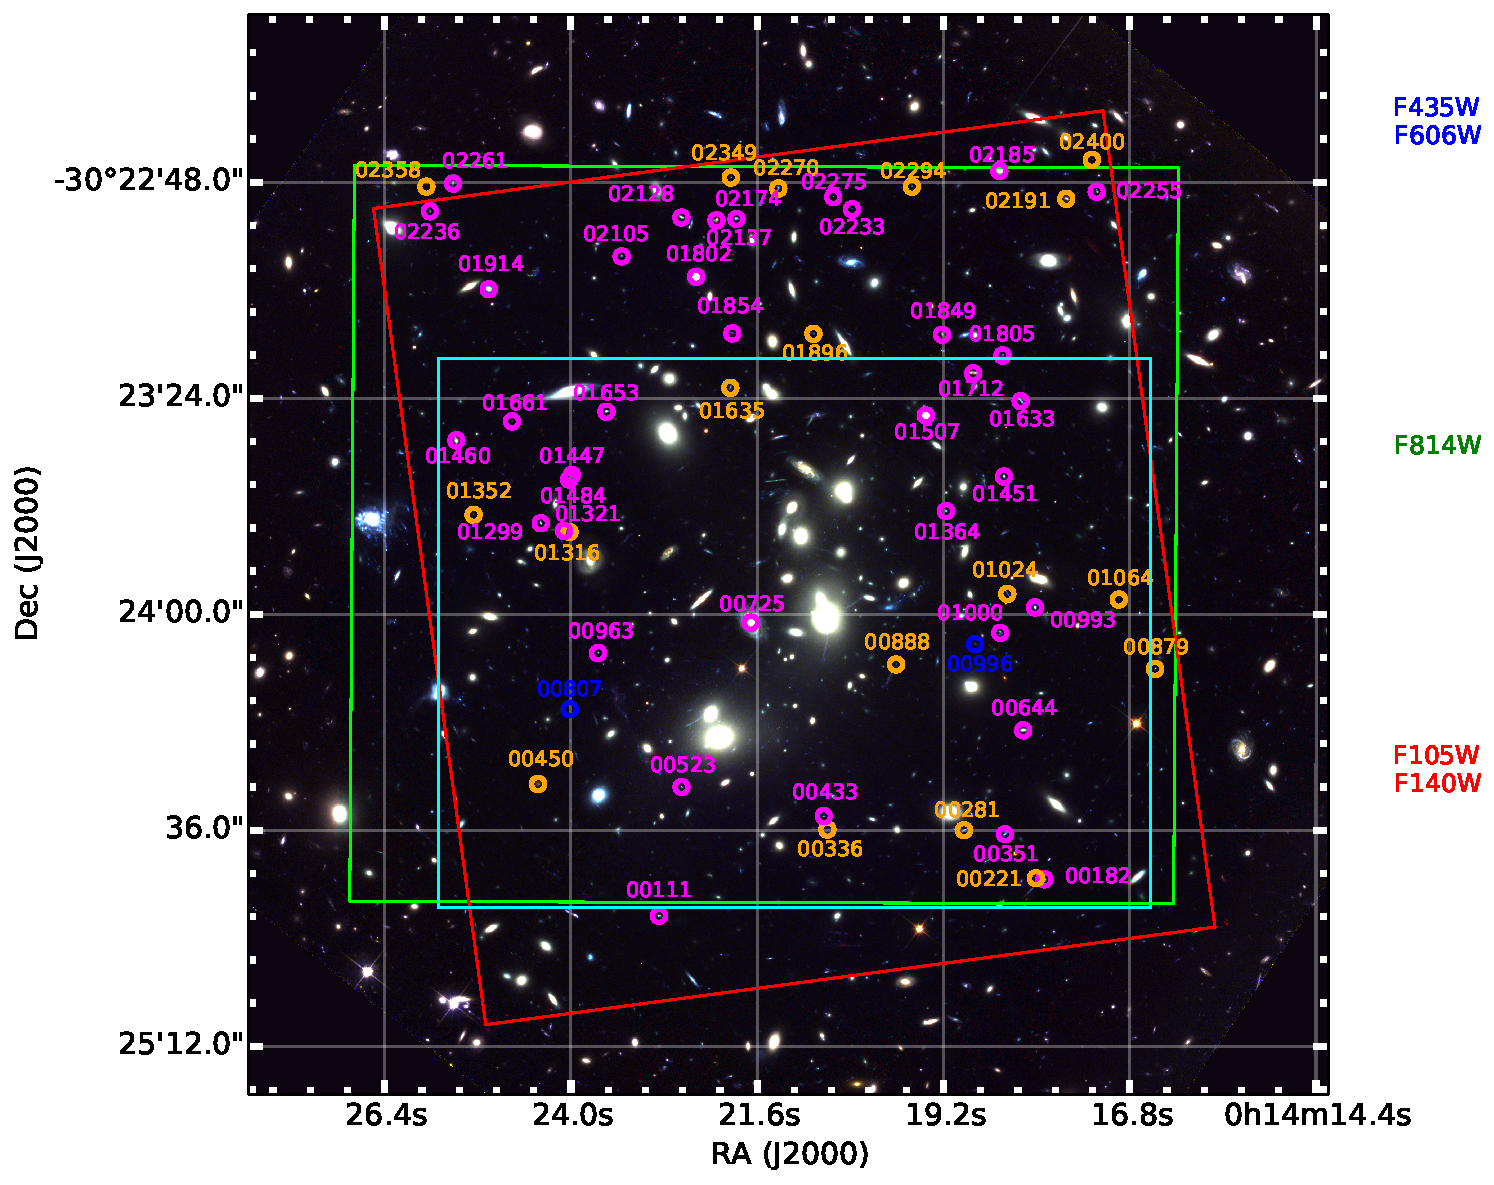
\includegraphics[width=\textwidth]{fig/A2744_RGB_final_byhandlabels.pdf}
    \caption[The color composite image of \cler based on the HFF and GLASS imaging.]{The color composite image of \cler based on the HFF and GLASS imaging. The blue, green and red channels are composed by 
the filters on the right. The two distinct P.A.s of the spectroscopic GLASS pointings are shown by the red (P.A.=233 degrees) and 
green (P.A.=135 degrees) squares. Figure~\ref{fig:grisms} shows the grism images corresponding to these two P.A.s. The locations 
of the emission line objects from Table~\ref{tab:ELtot} are marked by circles, with color coding reflecting the GLASS 
spectroscopic redshift quality (cf. Section~\ref{subsec:targeted} and column ``Quality'' in Table~\ref{tab:ELtot}; 2=blue, 
3=orange, and 4=magenta). The cyan square shows the outline of Figure~\ref{fig:arcs_image}.}
\label{fig:image}
\end{figure}

%= = = = = = = = = = = = = = = = = = = = = = = = = = = = = = = = = = = = = = = = 
\begin{figure}
    \includegraphics[width=0.5\textwidth]{fig/A2744_RGB_A2744-135-141027-G102_drz_final.pdf}
    \includegraphics[width=0.5\textwidth]{fig/A2744_RGB_A2744-135-141027-G141_drz_final.pdf}\\
    \includegraphics[width=0.5\textwidth]{fig/A2744_RGB_A2744-233-141027-G102_drz_final.pdf}
    \includegraphics[width=0.5\textwidth]{fig/A2744_RGB_A2744-233-141027-G141_drz_final.pdf}
    \caption[The GLASS G102 and G141 grism pointings of \cler at two distinct P.A.s.]{The GLASS G102 (left) and G141 (right) grism pointings of \cler at two distinct P.A.s, with field-of-view shown by the 
red (P.A.=233 degrees) and green (P.A.=135 degrees) squares. The circles in all panels denote the positions of the emission line 
objects identified in this work, with color coding following the convention adopted in Figure~\ref{fig:image}.}
\label{fig:grisms}
\end{figure}
%= = = = = = = = = = = = = = = = = = = = = = = = = = = = = = = = = = = = = = = = 

The GLASS observations are designed to follow the 3D-HST observing strategy \citep{Brammer:2012p12977}.
The data were processed with an updated version of the 3D-HST reduction pipeline\footnote{\url{http://code.google.com/p/threedhst/}}.  Below we summarize the main steps in the reduction process of the GLASS data but refer to 
\citet{Brammer:2012p12977} and \citet{Treu:2015p36793} for further details.

The data were taken in a 4-point dither pattern identical to the one
shown in Figure~3 of \cite{Brammer:2012p12977} to optimize rejection of bad pixels and cosmic rays
and improve sampling of the WFC3 point spread function.
At each dither position, a combination, a direct (F105W or F140W), and a grism (G102 or G141) exposure were taken.
The direct imaging is commonly taken in the filter ``matching'' the grism, i.e. pairs of F105W-G102 and F140W-G141.  However, to 
accommodate searches for supernovae and the characterization of their curves in GLASS clusters, each individual visit is designed 
to have imaging in both filters. Hence several pairs of F140W-G102 observations exist in the GLASS data. This does not affect the 
reduction and extraction of the individual GLASS spectra.
%due to the difference in sensitivity of the grisms, and hence the division between the orbits, 

The individual exposures were turned into mosaics using AstroDrizzle from the DrizzlePac \citep{Gonzaga:2014p26307}, the  
replacement for MultiDrizzle \citep{Koekemoer:2003p31861} used in earlier versions of the 3D-HST reduction pipeline. Then all  
exposures and visits were aligned using \verb+tweakreg+, with backgrounds subtracted from the direct images by fitting a second  
order polynomial to each of the source-subtracted exposures. We subtracted the backgrounds using the master sky presented by  
\cite{Kummel:2011p33451} for the G102 grism, while for the G141 data the master backgrounds were developed by  
\cite{Brammer:2012p12977} for 3D-HST. The individual sky-subtracted exposures were combined using a pixel scale of $0\farcs06$ per  
pixel as described by \citet{Brammer:2013p27911} ($\sim$half a native WFC3 pixel) which corresponds to roughly 12\AA/pixel and  
22\AA/pixel for the G102 and G141 grism dispersions, respectively. Figure~\ref{fig:grisms} shows these full field-of-view 
mosaics of the two NIR grisms (G102 on the left and G141 on the right) at the two GLASS P.A. for \cler. The  individual spectra 
were extracted from these mosaics by predicting the position and extent of each two-dimensional spectrum according to the 
\verb+SExtractor+ \citep{Bertin:1996p12964} segmentation maps from the corresponding direct images. This is done for every single 
object and contaminations, i.e., dispersed light from neighboring objects in the direct image, so these contaminations can be 
estimated and accounted for.

%========================================================================
\section{Identification of Multiple Images}
\label{sec:mul}

In this section we describe how we identify and vet multiple image
candidates using imaging (\ref{subsec:photometry}) and spectroscopic
(\ref{subsec:targeted} and \ref{subsec:blind}) data.

\subsection{Imaging Data: Identification and Photometric Redshifts}
\label{subsec:photometry}

\citet{2011MNRAS.417..333M} published the first detailed strong lensing analysis of \cler identifying a total of 34 multiple 
images  (11 source galaxies) in imaging data pre-dating the HFF. With the addition of the much deeper HFF data, now a total of 
176/56  candidate arc images/systems have been identified prior to this work \citep[][see also Figure~\ref{fig:arcs_image} and 
Table~\ref{tab:mult_images}]{2014ApJ...786...60A,2015ApJ...800...18A,2014ApJ...793L..12Z,2014MNRAS.444..268R,2014arXiv1409.8663J,2014ApJ...797...98L,Ish++15}.
We identify a new multiply imaged system (i.e. system 60 in Table~\ref{tab:mult_images}) comprised of three images. 

%= = = = = = = = = = = = = = = = = = = = = = = = = = = = = = = = = = = = = = = = 
\begin{figure}
    \centering
    \includegraphics[width=\textwidth]{fig/A2744_image.pdf}
    \caption[All multiple images discovered to date in \cler.]{All multiple images discovered to date in \cler.
        Green images are used in the lens model, while red images are unused for reasons discussed in
        Section~\ref{sec:mul}. Cyan images belong to a new multiple image system discovered in this work. The
        yellow line is the critical curve from our best-fit lens model at $z=9$. The RGB image is a combination
        of F105W, F125W and F160W. }
    \label{fig:arcs_image}
\end{figure} 
%= = = = = = = = = = = = = = = = = = = = = = = = = = = = = = = = = = = = = = = = 

Despite the vast number of identifications, only a handful of multiple images have been spectroscopically confirmed; arcs 4.3 and 
6.1 were spectroscopically confirmed by \citet{2014MNRAS.444..268R}, arcs 3.1, 3.2 and 4.5 by \citet{Joh++14}, and arc 18.3 by 
Cl\'{e}ment et al. (in preparation). All corresponding redshifts can be found in Table~\ref{tab:mult_images}.  When spectroscopy 
is lacking, confirming that images belong to the same source is much more difficult. Photometric redshifts alone are not adequate 
for confirmation.  \citet{Ilb++06} found that, within a given survey, the fraction of catastrophic errors in photometric redshift increases with faintness 
and redshift. Multiple images are typically faint and are necessarily at redshifts larger than the cluster redshift, which is 
$z=0.308$ for \cler. The mean F140W magnitude of all images in Table~\ref{tab:mult_images} is 27.11, and the mean source redshift 
is $z=2.63$. Photometry of sources in cluster fields is complicated due to blending with cluster members and the ICL.  While we do 
compute photometric redshifts in order to use the multiple images in our lens model, we do not rely on them alone to test the 
fidelity of the images.

We instead rely on color and morphology information to determine whether images belong to the same multiple image system; to first order, multiple images of the same source have identical colors. To compute colors, photometry is done using \verb+SExtractor+ in dual-image mode. We use F160W as the detection image because it detects the largest fraction of all multiple image candidates. We then measure isophotal magnitudes and errors 
in all seven photometric filters. Due to difficulties in detecting many of the multiple image candidates using the default \verb+SExtractor+ 
settings, we adopt a more aggressive set of settings for the objects with low $S/N$ and/or highly blended. We refer to the 
default \verb+SExtractor+ settings as ``cold'' mode and the more aggressive one as ``hot'' mode photometry. These are similar in spirit but not identical to those adopted by \citet{Guo+13}. Even with the ``hot'' mode settings, we cannot detect all of the multiple image candidates, though the detected fraction is vastly increased over the ``cold'' mode settings. 
Using the seven HFF photometric filters, we compute 4 colors for each image: 
$F435W-F606W$, $F814W-F105W$, $F125W-F140W$, and $F140W-F160W$\footnote{Note that the last two colors are not independent due to 
the repetition of $F140W$. We chose to repeat one filter to increase the number of color bins.}. The colors are computed 
within a fixed aperture (MAG\_APER) that is $0.4''$ in diameter. We compute a reduced ``color-$\chi^2$'' for each image:
\begin{equation}
  \chi^2_{I \nu}  = {1 \over N-1} \sum_{i=1}^{N} \left({C_i - \bar{C}_i \over \sigma_i} \right)^2,
\end{equation}
where $i$ runs over the number of colors, $N$ is the total number of colors we are able to measure, $C_i$ is the $i$-th color, 
$\bar{C_i}$ is the inverse variance-weighted mean color of all images in the system, and $\sigma_i$ is the uncertainty in the 
$i$-th color. 

Multiple images of the same source also have predictable morphologies. In rare cases, more than one images of the
same source possess a number of uniquely identifiable features. For instance, there are two such systems in
\cler, i.e., systems 1 and 2. The counterparts to systems 1 and 2 are systems 55 and 56, respectively. We include
both counterpart systems in the lens model at the spectroscopic redshifts of systems 1 and 2 that we measure in
this work. All multiple images in Table~\ref{tab:mult_images} are visually inspected. We assign each image a
grade that determines the likelihood that it is part of the system to which it is assigned.  We perform this
grading exercise in a lens model-independent fashion; we do not make any assumptions about the location of the
critical curves relative to the graded images. There are, however, configurations of multiple images that are
impossible to achieve through gravitational lensing by galaxy clusters, such as three individual images (not part
of an elongated arc) on the same side of, and very distant from the cluster core with no counter-images. Other
information such as surface brightness and symmetry can be incorporated independently of an assumed mass
distribution, and we rely on this information much more heavily in assigning the morphology grade.The grading
scheme based on morphological similarity is as follows:
\begin{description}
    \item[4] Image is definitely part of the system
	\item[3] Image is very likely part of the system
	\item[2] Image is potentially part of the system
	\item[1] Image is very unlikely part of the system
	\item[0] Image is definitely not part of the system
\end{description}

%\noindent
%Two inspectors independently assign a grade to each image. The inspectors use several
%RGB images of the full HFF depth that span the full HST spectral coverage to assign the grade for each image. The
%two grades are then summed to get the reported morphology grade. 

We use the color and morphology information together to determine whether to include a multiple image in our
model. The joint criteria are: \begin{equation} (\chi^2_{I \nu} < 1.5 \quad \lor \quad \textrm{M} > 5) \quad
\land \quad M>0, \end{equation} where M is the summed morphology grade from each inspector, which ranges from
0-8. In cases where the contamination by foreground objects, clusters members or ICL is severe, we rely only on
the morphology criterion, $M>5$. The particular $\chi^2_{I \nu}$ threshold value of $1.5$ was chosen because it
is in the typical range for a good reduced chi-square test, and most of the images in spectroscopically confirmed
systems are below this value. $M>5$ is chosen because in the least confident case that obeys this, $M=6$, the
modelers either both think the image is very likely part of the system ($M=3$) or one thinks the image is
potentially part of the system ($M=2$), while the other is sure of it ($M=4$). 

For a multiple image system to constrain the lens model, we must
estimate its redshift. Having photometric redshift measurements for
multiple images of the same source can provide a tighter constraint
than a single measurement. Individual photometric redshifts are
computed using EAZY \citep{Brammer:2008p13280}. We then use a
hierarchical Bayesian model to obtain a single redshift probability
density function for each system \citep{Dahlen:2013p33380}. The mode
of this probability density function will be referred to as
$z_{\textrm{Bayes}}$. Only non-contaminated objects contribute to
calculating $z_{\textrm{Bayes}}$. We graphically outline the procedure
for measuring and including photometric redshifts as inputs to our
lens model in Figure~\ref{fig:flow_chart}. 2/57 systems (36 and 52) are
entirely contaminated, so we do not compute $z_{\textrm{Bayes}}$ for
those systems. 14/57 systems have $z_{\textrm{Bayes}} <
z_{\textrm{Cluster}}$, and thereby are not included in lens modeling (a
fraction of those have poorly constrained posteriors, monotonically
declining from 0; they are highly uncertain and considered unreliable;
we label them by assigning $z_{\rm Bayes}=0.01$). 5/57 systems have a
multi-modal or extremely broad Bayesian redshift distribution. We similarly do
not include these systems in the lens modeling. For systems where only one image passed the
color/morphology criteria and that image is not contaminated, we report
$z_{\textrm{Bayes}}$ in Table~\ref{tab:mult_images}, but we do not
include these systems in the modeling. We show the posterior redshift
distributions for some of these cases in the Appendix. System 18
consists of a spectroscopically confirmed image (18.3), but the system as
a whole does not pass all criteria required to be considered a
multiple image system. Our screening rules out all the above-mentioned
systems and delivers a secure set of 25/57 multiple arc systems that
are used in lens modeling.

%= = = = = = = = = = = = = = = = = = = = = = = = = = = = = = = = = = = = = = = = 
\begin{figure}
    \centering
    \includegraphics[width=.8\textwidth]{fig/Photo-z_flow_chart.pdf}
    \caption[Flow chart describing our procedure for assigning photometric redshifts to multiple image
    systems.]{Flow chart describing our procedure for assigning photometric redshifts to multiple image systems.
    Two segmentation maps, a ``hot'' and a ``cold'' version, were used for source detection. The detection and
    deblending thresholds are set to the SExtractor defaults in the cold segmentation map. Objects detected in
    the cold segmentation map, typically the brighter and more isolated ones, have more accurate photometry. The
    hot segmentation map was created using extremely aggressive detection and deblending thresholds. It detects
    the majority of the remaining multiple images that are not detected in the cold version.
    $\textrm{C}/\textrm{M}$ cuts refer to the color/morphology cuts used to purify the sample of multiple images.
    $z_{\mathrm{Bayes}}$ refers to the redshift obtained from combining multiple redshifts in a hierarchical
    Bayesian model \citep{Dahlen:2013p33380}. $z_{\mathrm{Bayes}}$ is considered reliable if it is larger than
    the redshift of \cler, $z=0.308$, and it is not multi-valued. See the Appendix for examples of multiple image
    systems that pass and fail some of the tests in this flow chart. }
    \label{fig:flow_chart}
\end{figure} 
%= = = = = = = = = = = = = = = = = = = = = = = = = = = = = = = = = = = = = = = = 

\subsection{Targeted \glass Spectroscopy}
\label{subsec:targeted}

GLASS spectroscopy was carefully examined for a total of \NimgTOT{}
multiply lensed arc candidates mostly seen on both P.A.s with the goal
of measuring spectroscopic redshifts.
Each spectrum was visually inspected by multiple investigators
using the GLASS Graphic User Interfaces (GUIs) GLASS
Inspection GUI (GiG) and GLASS Inspection GUI for redshifts (GiGz) The
results were then combined and a preliminary list of arcs with
emission lines was drafted. In the end, another round of double-check
by re-running GiGz was also executed to make sure no potential
emission lines were missed. Following GLASS procedure, a quality flag
was given to the redshift measurement: Q=4 is secure; Q=3 is probable;
Q=2 is possible; Q=1 is likely an artifact.
These quality criteria take into account the signal to noise ratio of
the detection, the probability that the line is a contaminant, and the
identification of the feature with a specific emission line. For
example, Q=4 is given for spectra where multiple emission have been
robustly detected; Q=3 is given for spectra where either a single
strong emission line is robustly detected and the redshift
identification is supported by the photometric redshift, or when more
than one feature is marginally detected; Q=2 is given for a single
line detection of marginal quality. As shown in Table~\ref{tab:ELtot},
new spectroscopic redshifts were obtained for \NimgELtot{} images in
total, corresponding to \NsysELtot{} systems. Among them, \NimgELhiQ{}
high-confidence (with quality flags 3 or 4) spectroscopic redshifts
were measured for arcs 1.3, 6.1, 6.2, 6.3, 56.1. The spectra of these
objects are shown in
Figures~\ref{fig:ELarc6.1}--\ref{fig:ELarc56.1}. In particular for arc
6.1, our spectroscopic redshift matches that reported by
\citet{2014MNRAS.444..268R}, and we provide the first spectroscopic
confirmation that 6.2 and 6.3 are images of the same system.

We note that our measured redshift for arc 56.1 $z_{\textrm{spec}}=1.20$ (Q=3; probable) differs signficantly
from that given by \citet{Johnson:2014p37801} for arc 2.1 $z_{\textrm{spec}}=2.2$ (possible), even though the two
systems are likely to be physically connected.  Our measurement is based on three pieces of evidence. First, we
detect a spectral feature in G141 at both P.A.s (see Figure~\ref{fig:ELarc56.1} for details) with sufficiently
high signal to noise ratio to study its spectra shape. The feature is better described by a single line
(identified by us as \Ha at $z=1.2$) rather than a doublet like \OIII ($\Delta \chi^2=2.4$). Second, a
line is marginally detected in one of the G102 spectra at exactly the wavelength expected for \OIII $z=1.2$.
Third, the wide spectral coverage of our data and the data available in the literature rule out the possibility
of the feature we see in G141 being other prominent lines such as Mg II and \OII. Taking into account both the
evidence and previous results, we assign a quality flag of Q=3 (probable).

The uncertainty on our spectroscopic redshift measurements is limited
by the resolution of approximately 50\AA and by uncertainties in the
zero point of the wavelength calibration. By comparing multiple
observations of the same object we estimate the uncertainty of our
measurements to be in the order of $\Delta z\sim 0.01$. This is
sufficient for our purposes and we will not pursue more aggressive
approaches to improve the overall redshift precision
\citep[e.g.][]{Brammer:2012p12977}.

% = = = = = = = = = = = = = = = = = = = = = = = = = = = = = = = = = = =
\begin{figure}
    \centering
    \includegraphics[width=.8\textwidth]{fig/clA2744_id963_pa135_zsQ4.pdf}\\
    \includegraphics[width=.8\textwidth]{fig/clA2744_id963_pa233_zsQ4.pdf}
    \caption[Emission line detection results on object ID 00963 (arc 6.1).]{Emission line detection results on object ID 00963 (arc 6.1) at the two P.A.s displayed in the two
    sub-figures accordingly. In each sub-figure, the two panels on the first row show the observed 1-dimensional
    spectra, where the contamination subtracted flux is denoted by the blue solid line and the noise level by the
    cyan shaded region. The two panels on the second row give the corresponding contamination model in red dashed
    line. For the four panels directly underneath, the top two display the interlaced 2-dimensional spectra
    whereas the bottom two have contamination subtracted. In the 1- and 2-dimensional spectra, the identified
    emission lines are denoted by vertical dashed lines in magenta and arrows in red, respectively. The wheat
    colored regions cover contamination model defects. The two panels on the far left refer to the 2-dimensional
    postage stamp created from the HFF co-adds through drizzling (on top) and the 1-dimensional collapsed image
    (on bottom). Note that these two panels share the same x-axis along the grism dispersion direction. Some
    ancillary information can also be seen in the upper left corner in each sub-figure.\label{fig:ELarc6.1}}
\end{figure}

\begin{figure}
    \centering
    \includegraphics[width=\textwidth]{fig/clA2744_id523_pa135_zsQ4.pdf}\\
    \includegraphics[width=\textwidth]{fig/clA2744_id523_pa233_zsQ4.pdf}
    \caption{Same as Figure~\ref{fig:ELarc6.1}, except that object ID 00523 (arc 6.2) is shown.}
    \label{fig:ELarc6.2}
\end{figure}

\begin{figure}
    \centering
    \includegraphics[width=\textwidth]{fig/clA2744_id433_pa135_zsQ4.pdf}\\
    \includegraphics[width=\textwidth]{fig/clA2744_id433_pa233_zsQ4.pdf}
    \caption[Same as Figure~\ref{fig:ELarc6.1}, except that object ID 00433 (arc 6.3) is shown.]{Same as
    Figure~\ref{fig:ELarc6.1}, except that object ID 00433 (arc 6.3) is shown. Note here WFC3/G102 at the
    second P.A. is cut off on the right due to grism defect.}
    \label{fig:ELarc6.3}
\end{figure}

\begin{figure}
    \centering
    \includegraphics[width=\textwidth]{fig/clA2744_id336_pa135_zsQ3.pdf}\\
    \includegraphics[width=\textwidth]{fig/clA2744_id336_pa233_zsQ3.pdf}
    \caption[Same as Figure~\ref{fig:ELarc6.1}, except that object ID 00336 (arc 1.3) is shown.]{Same as Figure~\ref{fig:ELarc6.1}, except that object ID 00336 (arc 1.3) is shown. Moreover, the 2-dimensional
  spectra are smoothed, whilst the 1-dimensional spectral resolution remains unchanged.}
    \label{fig:ELarc1.3}
\end{figure}

\begin{figure}
    \centering
    \includegraphics[width=\textwidth]{fig/clA2744_id888_pa135_zsQ3.pdf}\\
    \includegraphics[width=\textwidth]{fig/clA2744_id888_pa233_zsQ3.pdf}
    \caption{Same as Figure~\ref{fig:ELarc1.3}, except that object ID 00888 (arc 56.1) is shown.}
    \label{fig:ELarc56.1}
\end{figure}
% = = = = = = = = = = = = = = = = = = = = = = = = = = = = = = = = = = =


\subsection{Blind Search in GLASS Data}
\label{subsec:blind}

The targeted spectroscopy done in Section~\ref{subsec:targeted} could
potentially miss some multiply imaged sources that are not identified
photometrically. In order to increase the redshift completeness of
emission line sources (both multiply and singly imaged), we also
conducted a blind search within the entire grism field-of-view. As a
first step, we visually inspected all the 2D grism
spectroscopic data, the contamination models, and residuals after
contamination for each of the 2445 objects in the prime filed of \cler
given by the GLASS catalog.  This yielded a list of 133 candidate
emission line systems that were later on inspected using the GLASS
GUIs GIG and GIGz to confirm emission
line identifications and measure redshifts.  In order to search for
previously undiscovered multiple images we inspected each set of
objects with mutually consistent redshift.  None of the sets of
galaxies at the same spectroscopic redshifts are consistent with being
multiply lensed images of the same source. Some of them are ruled out
because of their position in the sky, while others are ruled out
because their colors and morphology are inconsistent with the lensing
hypothesis.

Nonetheless, we compiled a list of singly imaged emission line
objects, consisting of \NELQtwo{}, \NELQthree{}, and \NELQfour{}
quality 2, 3, and 4 spectroscopic redshift measurements respectively,
which are color coded in Figure~\ref{fig:image}. Among them, the
high-confidence (with quality flag 3 or 4; orange and magenta circles
in Figure~\ref{fig:image}) emission line identifications are also
included in Table~\ref{tab:ELtot}. As mentioned in
Section~\ref{subsec:photometry}, via running EAZY on the full-depth
seven-filter HFF imaging data, we were able to measure photometric
redshifts for those objects as well. As a result, a comparison between
spectroscopic and photometric redshift measurements is possible, as
displayed by Figure~\ref{fig:ELobjs_photz}. We find that 25/55
photometric redshifts agree within their 1-$\sigma$ uncertainties with
corresponding spectroscopic redshifts, when nebular emission lines are
included in the fitting template. This suggests the presence of
additional systematic errors that are likely related to the
photometric redshift fitting method. In order to account for the
unknown systematics, we increase the photometric redshift
uncertainties for the sources used in the construction of the lens
model.

We double-checked our spectroscopic redshift measurements by
re-running GiGz on all the objects and also cross-checked the photometric
redshift measurements through re-fitting the photometric redshifts
using a different method by a subset of the authors (R.A., M.C., E.M)
without knowing previous results. The general conclusions about the
agreement between spectroscopic and photometric analyses remains
unchanged.

% = = = = = = = = = = = = = = = = = = = = = = = = = = = = = = = = = = =
\begin{figure}
    \centering
    \includegraphics[width=\textwidth]{fig/a2744_ELobjs_photz_vs_specz.pdf}
    \caption[Comparison between the spectroscopic and photometric redshifts.]{Comparison between the spectroscopic and photometric redshifts for the 55 objects with
    high-confidence emission lines (quality flags 3 or 4).  We also show the 1-$\sigma$ error bars (enclosing
    68\% of the total probability) around the photometric redshifts. There is reasonably good agreement between
    photometric and spectroscopic redshifts, with 25 out of 55 spectroscopic redshifts within the photometric
    redshift error bars. This is acceptable considering that the photometric redshift uncertainties only include
    the random component, even though they suggest that an additional systematic uncertainty component is
    present. In order to account for this systematic uncertainty, for the systems used to build the lens model we
    added 20\% in quadrature to our photometric errors.  \label{fig:ELobjs_photz}}
\end{figure}
% = = = = = = = = = = = = = = = = = = = = = = = = = = = = = = = = = = =

\section{Gravitational Lens Model}
\label{sec:mass}

Our lens modeling method constrains the gravitational potential within a
galaxy cluster field via $\chi^2$ minimization. It takes as input a
simple initial model for the potential. A $\chi^2$ is then calculated
from strong and weak gravitational lensing data on an adaptive,
pixelated grid over the potential established by the initial
model. The number of grid points is increased and the $\chi^2$ is
recalculated. Once the minimum is found, and convergence is achieved,
derivative lensing quantity maps, such as convergence ($\kappa$),
shear ($\gamma$) and magnification ($\mu$), are produced from the
best-fit potential map. Errors in these quantities are obtained via the method described below.
Maps of the convergence and magnification
are shown in Figure~\ref{fig:lens_maps}.

% = = = = = = = = = = = = = = = = = = = = = = = = = = = = = = = = = = 
\begin{figure}
    \includegraphics[width=0.5\textwidth]{fig/kappaplanck.pdf}
    \includegraphics[width=0.5\textwidth]{fig/magplanck.pdf}
    \caption[Convergence and magnification of our lens model.]{Convergence (left), $\kappa$ and flux magnification (right), $\mu$, maps of \cler produced by our
    lens model for a source at $z=9$. Maps cover $3.5 \times 3.5 \, \textrm{arcmin}^2$. In both maps, the gray
    stick pattern indicates the phase angle of the shear. \label{fig:lens_maps}}
\end{figure}
% = = = = = = = = = = = = = = = = = = = = = = = = = = = = = = = = = = =

A previous model of \cler using pre-HFF data was created using the same lens modeling code. The model was created
as part of a call by STScI to model the HFF clusters, and it appears on the publicly accessible HFF lens modeling
website as the bradac v1
models\footnote{\url{http://www.stsci.edu/hst/campaigns/frontier-fields/Lensing-Models}}. The previous model was
constrained using 44 total multiple images belonging to 11 distinct systems. The weak lensing constraints were
obtained by one of the modelers, Julian Merten, and distributed to all participating modeling teams. The same
weak lensing constraints were used in the model that appears in this work. This model is also made available to
the public on the HFF lens modeling website as the bradac v2 model.  In the v1 model, magnification uncertainties
were estimated by bootstrap-resampling the weak lensing galaxies. In this work, however, we took a different
approach to estimate uncertainties, one that we expect more accurately represents the true uncertainties.
Because the number of multiple image systems used in this model is much larger than in the v1 model, 72 total
multiple images belonging to 25 distinct systems, we bootstrap-resampled the multiple image systems that were not
spectroscopically confirmed.  These are the systems for which we use $z_{\textrm{Bayes}}$ in the lens model.
We assess the impact of photometric redshift uncertainty on the derived lensing quantities by resampling
the redshift of each system lacking spectroscopic confirmation from their full $z_{\textrm{Bayes}}$
posteriors\footnote{We exclude values of the redshift $z<z_{\textrm{cluster}}+0.1$ when resampling from the
$z_{\textrm{Bayes}}$ posteriors because they are unphysical.}. We compare the variance in magnification due to
redshift uncertainty with the variance in magnification due to bootstrap-resampling the multiple image systems,
finding that the latter is dominant. We nonetheless propagate both sources of error when reporting the errors on
all derived lensing quantities in this work.

As a test of the improvement of the lens model with the addition of the new multiple image constraints from the
HFF data, we calculate the magnification of SN HFF14Tom, a Type Ia Supernova (SN Ia) at $z=1.35$ discovered in
the primary cluster field of \cler (\citealp{Rod++15}). We compare the magnification predicted by our lens model
with the magnification calculated directly from a comparison with other SNe Ia at similar redshifts,
$\mu=2.03\pm0.29$ (\citealp{Rod++15}). The magnification predicted by the v1 model, using pre-HFF data was
$\mu_{\mathrm{best}} = 3.15$, with $\mu_{\mathrm{median}} = 2.45^{+0.19}_{-0.16}$ ($68\%$ confidence).
The new model presented in this work, v2, predicts a consistent magnification of $\mu_{\mathrm{best}} =
2.23$, with $\mu_{\mathrm{median}} = 2.24^{+0.07}_{-0.08}$ ($68\%$ confidence). The improved lensing constraints
significantly improve the accuracy as well as the precision according to this test. We note that while we were
not blind to the magnification of the supernova predicted by \citet{Rod++15} when producing the v2 lens model, we
did not use the magnification as an input to our model. 

\subsection{Comparison with Previous Work}
\label{sec:compare}

Three teams (\citealp{2014arXiv1409.8663J}, \citealp{2014ApJ...797...98L} and
\citealp{Ish++15}) have published models of \cler using new multiple
image constraints identified in the HFF imaging data. Of these teams,
currently only the lens models produced by \citealp{Ish++15} (GLAFIC) are
publicly available through the Mikulski Archive for Space Telescopes
(MAST\footnote{\url{http://archive.stsci.edu/prepds/frontier/lensmodels/}}). We
compare our models to theirs as well as the Sharon v2 models, which
include updated spectroscopic measurements of multiple images
identified before the HFF data were obtained (\citealp{Joh++14}). Finally, we also compare our model with 
several updates of the CATS(v1) models (Jauzac et al. 2015, private
communication). The CATS(v2) models are presented by \citet{2014arXiv1409.8663J} and use a much larger number of multiple images than we include in our lens model. CATS(v2.1) employs the same set of multiple images as CATS(v2), but makes use of the spectroscopic redshifts obtained in this work. CATS(v2.2) uses the same set of multiple image constraints used in our model. We compare the surface mass density
profiles (Figure~\ref{fig:surfcompare}) and cumulative magnified source plane areas
(Figure~\ref{fig:area}) predicted by all models described above. The surface mass density profiles agree quite
well at radii where multiple image constraints are plentiful. However,
the models begin to differ rapidly near the boundaries of the
constrained area. Our model disagrees with the CATS models most severely. It is interesting to note that the three CATS models agree internally extremely well, despite CATS(v2.2) using the same set of multiple images used in this work, a considerably different set than the one used in CATS(v2) and CATS(v2.1). The significant difference between our model and the CATS models may be due to differences in the modeling techniques or the fact that our method uses additional constraints (weak lensing). Weak lensing constraints have a stronger impact on the model at radii beyond where multiple images are observed. In contrast, there is excellent agreement among the
models in the inferred magnified source plane area. Thus, even though
there may be small but significant differences in the specific details
of each reconstructions, by and large the total integrated properties
are very similar. 

We also note that our model supersedes the model obtained by members
of our team as part of the initial HFF modeling effort based on
pre-HFF data. The uncertainties in this current version of the model
are smaller, consistent with the fact that we have increased
the number of strong lensing constraints.

% = = = = = = = = = = = = = = = = = = = = = = = = = = = = = = = = = = =
\begin{figure}
    \centering
    \includegraphics[width=\textwidth]{fig/surface_mass_density_profile.pdf}
    \caption[Surface mass density profile of our lens model.]{Surface mass density profile for the lens model obtained in this work compared to several recently published lens 
        models of \cler. The Sharon v2 model is presented by \citet{Joh++14}, the GLAFIC model by \citet{Ish++15}, the CATS(v2) 
        model in \citet{2014arXiv1409.8663J}, and the CATS(v2.1) and CATS(v2.2) models by Jauzac et al. (2015, private 
        communication).  The shaded gray region indicates the radii over which multiple image constraints are available. The 
        models agree best within this region, and they begin to significantly disagree at radii $\gtrsim 200$kpc. The radius is 
        measured from the center of the BCG. Error bars shown for our model represent $68\%$ confidence. Gaussian 1-$\sigma$ error 
        bars are included on all three CATS models, but are almost entirely too small to discern.
\label{fig:surfcompare}}
\end{figure}
% = = = = = = = = = = = = = = = = = = = = = = = = = = = = = = = = = = =


%= = = = = = = = = = = = = = = = = = = = = = = = = = = = = = = = = = = = = = = = 
\begin{figure}
    \centering
    \includegraphics[width=\textwidth]{fig/cumulative_area_arcmin2_A2744.pdf}
    \caption[Cumulative source plane area versus magnification at $z=9$.]{Cumulative source plane area versus magnification at $z=9$. The models used in this comparison are the same as those 
    described in Figure~\ref{fig:surfcompare}.  \label{fig:area}}
\end{figure} 
%= = = = = = = = = = = = = = = = = = = = = = = = = = = = = = = = = = = = = = = = 

We also compare our method of estimating redshifts of multiple image
systems with the one used by the CATS team (\citealp{2014MNRAS.444..268R}, \citealp{2014arXiv1409.8663J}). In 
Figure~\ref{fig:compare_z}, $z_{\textrm{Bayes}}$ is the redshift
obtained from hierarchical Bayesian modeling of the photometric
redshifts obtained in this work. $z_{\textrm{model}}$ is the redshift
obtained by \citet{2014arXiv1409.8663J} by minimizing their analytical
model uncertainty while leaving the redshift as a free parameter. It
is important to check this procedure independently since leaving
$z_{\textrm{model}}$ as a free parameter or predicting additional
multiple images that belong to the same system could in principle lead
to confirmation bias. Overall, we find good agreement between
$z_{\textrm{Bayes}}$ and $z_{\textrm{model}}$, within the admittedly
large uncertainties on $z_{\textrm{Bayes}}$. There are only two new
systems with spectroscopic redshifts available to compare with
$z_{\textrm{model}}$, and they are both inconsistent at $>5\sigma$. This may be due to small
number statistics or perhaps an indication that the uncertainties on
$z_{\textrm{model}}$ are underestimated. More spectroscopic redshifts
are needed to perform this test in a more stringent manner.

% = = = = = = = = = = = = = = = = = = = = = = = = = = = = = = = = = = =
\begin{figure}
    \centering
    \includegraphics[width=.8\textwidth]{fig/redshift_comparison.pdf}
    \caption[Comparison of the redshifts estimates.]{Comparison of the redshifts determined in this work
    ($z_{\textrm{Bayes}}$) versus the model-predicted redshifts given by \citet{2014arXiv1409.8663J} for all
    multiple image systems used in the lens model. Note that the previously confirmed spectroscopic systems are
    left out of this comparison because $z_{\textrm model}$ were not calculated. Two systems (green) are
    spectroscopically confirmed in this work for the first time and are included in the comparison. For these two
    objects, we use the new spectroscopic redshift on the horizontal axis in place of $z_{\textrm{Bayes}}$. The
    $z_{\textrm{model}}$ values are in significant disagreement with the spectroscopic values for these two
    systems. $z_{\textrm{Bayes}}$ represents the peak of a statistical combination of all available photometric
    redshift probability density functions \citep{Dahlen:2013p33380}. The vertical error bars reflect 1-$\sigma$
    Gaussian error on $z_{\textrm{model}}$, and the horizontal error bars show the $68\%$ credible interval for
    $z_{\textrm{Bayes}}$. 12/16 systems are consistent at $68\%$ confidence level. }
    \label{fig:compare_z}
\end{figure}
% = = = = = = = = = = = = = = = = = = = = = = = = = = = = = = = = = = =


\section{The Spatial Distribution of Stellar and Dark Matter}

\subsection{Stellar Mass Map}

The \spitzer IRAC $3.6\,\mu$m image samples close to rest-frame
$K$-band for the cluster, so we use the $3.6\,\mu$m fluxes from
cluster members to approximate the cluster stellar mass
distribution. We first selected the red sequence cluster members
brighter than the 25th mag in F814W from the color-magnitude and
color-color diagrams following the procedure described in
\cite{2014MNRAS.444..268R}. We also cross-matched the selected cluster
members with the spectroscopic redshift catalog given by
\citet{Owers:2011ez} to ensure that we included all the cluster
members confirmed with spectroscopy.  We selected a total of 190
bright cluster members for their stellar mass distribution.

To create an image with $3.6\,\mu$m flux from cluster members only, we
first created a mask with value 1 for pixels that belong to cluster
members in the F160W image and 0 otherwise. We then convolved the mask
with the $3.6\,\mu$m PSF to match the IRAC angular resolution, set the
pixels below 10\% of the peak value to zero, and resample the mask
onto the IRAC pixel grid. We obtained the $3.6\,\mu$m map of cluster
members by setting all IRAC pixels not belonging to cluster members to
zero and smoothed the final surface brightness map with a two-pixel
wide Gaussian kernel.

The IRAC surface brightness map was transformed into a surface mass
density map by transforming the 3.6$\mu$m flux into K-band luminosity
and then by multiplying by stellar mass to light ratio derived by
\cite{B+d01} using the so-called ``diet''-Salpeter stellar initial 
mass function (IMF). The resulting stellar mass map in show in the
left panel of Figure~\ref{fig:stellarMassMap}.

The main source of uncertainty on the stellar mass density is the
unknown initial mass function. For example, if one were to adopt a
\cite{Sal55} IMF -- as suggested by studies of massive early-type
galaxies, the stellar mass density would increase by a factor of 1.55.

\subsection{Stellar to Total Mass Ratio}

We obtain the stellar to total mass ratio map by dividing the stellar
surface mass density map obtained from photometry by the total surface
mass density map obtained from gravitational lensing. This is shown in
the right panel of Figure~\ref{fig:stellarMassMap}. We note that
resolution effects are non-trivial to take into account, since the
resolution of the lensing map depends on the density of local sources
and the amount of regularization. Thus, the map should be interpreted
keeping in mind this caveat. Interestingly the stellar to total mass
ratio varies significantly across the cluster. Many but not all the
massive ellipticals seem to reach values of 0.05 or more, which are
typical of the central regions of isolated massive galaxies
\cite[e.g.][]{Gav++07}. However, the ratio appears to be significantly lower in the center of the cluster and in the south-east 
quadrant. In future work, we plan to compare the observed map with
those obtained from numerical simulations by taking into account the
effects of finite resolution in the observed mass and light maps, in
order to test whether the spread in stellar to total mass ratio is
reproduced. Furthermore, we plan to carry out a systematic comparison
with mass reconstructions where mass is assumed to follow light up to
a scale factor \citep{Zit++09}. At face value our result is
inconsistent with this assumption for a merging cluster like \cler. However,
uncertainties on both models and resolution effects must be taken into
account in order to evaluate the significance of this apparent
violation. Thus, this result should be considered as preliminary until
confirmed by a more detailed analysis.

%= = = = = = = = = = = = = = = = = = = = = = = = = = = = = = = = = = = = = = = = 
\begin{figure}
    \includegraphics[width=0.5\textwidth]{fig/a2744_clmember_smass_map_kpc2.pdf}
    \includegraphics[width=0.5\textwidth]{fig/total_stellar_mass_ratio_A2744.pdf}
    \caption[Stellar mass surface density and stellar to total mass ratio.]{Stellar mass surface density (left) and stellar to total mass ratio (right) distributions of \cler.
    Stellar mass surface density is in the unit of $M_\odot\,\text{kpc}^{-2}$.  \label{fig:stellarMassMap}}
\end{figure} 
\vspace{1cm}
%= = = = = = = = = = = = = = = = = = = = = = = = = = = = = = = = = = = = = = = 

%========================================================================
\section{Conclusions}
\label{sec:conc}

We have used spectroscopic data from the GLASS survey in
combination with ultra-deep imaging data from the HFF program to
construct a strong gravitational lens model for the cluster \cler. In an
effort to obtain a precise and accurate mass model we carried out a
systematic search for spectroscopic redshifts of multiple images and
we applied a rigorous algorithm to select only secure multiple image
systems amongst the dozens that have been proposed in the
literature. The lensing mass map is then combined with a stellar
mass map derived from IRAC photometry to study the relative spatial
distribution of luminous and dark matter.  Our main results can be
summarized as follows:

\begin{enumerate}

\item  We have measured spectroscopic redshifts for \NimgELhiQ{} multiple image systems (quality flag 4 and 3, i.e. secure and 
  probable). We have also confirmed spectroscopically that images 6.1, 6.2, 6.3 belong to the same source. The spectroscopically confirmed images are used to constrain the gravitational lens model. We also obtain 2 tentative redshifts, which are not used to 
  to constrain the mass model, but could potentially be confirmed by future work.

\item From the GLASS data we derive an extensive
redshift catalog of faint emission line systems which we use to test
photometric and lensing determinations of redshift. Generally
speaking, the measurements agree within the 1-$\sigma$ uncertainties,
when nebular emission lines are included in the fitting template.  In
addition, we compare photometric redshifts with redshifts determined
by \citet{2014arXiv1409.8663J}, based on their gravitational lens model and
find an agreement within the large uncertainties of the former. For
the two systems with new spectroscopic redshifts we find a significant
difference with respect to model redshifts. This may be due to small
number statistics or to the model redshifts uncertainties being
underestimated. More spectroscopic redshifts are needed to make a more
stringent test.

\item Our rigorous selection algorithm identifies a total of 25/72 multiple arc systems/images as secure out of a sample of 57/179 
  candidate multiple arc systems/images, compiled from the literature
  and from our own work. Most systems are rejected either on the basis
  of inconsistent morphology or inconsistent spectral energy
  distribution between the candidate multiple images, or because of
  insufficient evidence that they belong to the same source.

\item The derived mass model is found to be very precise, as measured by bootstrap- and redshift-resampling the set of multiple images used as 
  input. Furthermore, we tested how well our model reproduces the magnification of the background SN Ia Tomas (\citealp{Rod++15}). The SN Ia was not used as a constraint to the model and yet its magnification is consistent 
  ($2.03 \pm0.29$ for the supernova vs 2.23$^{+0.08}_{-0.07}$ from our mass model). 

\item \cler is confirmed to be an excellent gravitational telescope, with a source plane area of $\sim0.7$ arcminute square being 
  magnified by a factor of 2.

\item We construct a stellar surface mass density map and the stellar to total mass ratio by selecting the light associated with red sequence cluster galaxies and using the total mass density map obtained from strong lensing. Albeit with significant uncertainties, we find that the stellar to mass ratio varies significantly across the cluster, tentatively suggesting that stellar mass does not trace total mass in this interacting system.

\end{enumerate}

%%= = = = = = = = = = = = = = = = = = = = = = = = = = = = = = = = = = = = = = = = 

% = = = = = = = = = = = = = = = = = = = = = = = = = = = = = = = = = = = = = = = = = =
% Include this table with \input{filename.tex}
% To rotate in emulateapj do: \begin{turnpage}\input{filename.tex}\end{turnpage}
% To display it on multiple pages do: \LongTables\input{filename.tex}
% - - - - - - - - - - - - - - - - - - - - - - - - - - - - - - - - - - - - - - - - - -
%\newcolumntype{L}[1]{>{\raggedright\let\newline\\\arraybackslash\hspace{5pt}}m{#1}}
%\begin{deluxetable}{L{4em}ccccccccccccc} \tablecolumns{13}
\begin{deluxetable}{rccccccccccccc}
    \tablecolumns{13}
    \tabletypesize{\scriptsize}
    \tabcolsep=0.08cm
    \tablewidth{0pt}
    \tablecaption{Multiply lensed arc systems identified in the \cler field\label{tab:mult_images}}
% - - - - - - - - - - - - - - - - - - - - - - - - - - - - - - - - - - - - - - - - - -
\tablehead{
  \colhead{ID$_\textrm{arc}$\tablenotemark{1}} &
  \colhead{R.A.} &
  \colhead{Dec.} &
  \colhead{F140W} &
  \colhead{$z_{\textrm{spec}}$} &
  \colhead{$z_{\textrm{Bayes}}$\tablenotemark{2}} &
  \multicolumn{4}{c}{Quality} &
  \multicolumn{2}{c}{Pass Flag} &
  \colhead{Magnification\tablenotemark{4}} \\
  & (deg.) & (deg.) & (mag) & & & \multicolumn{4}{c}{\hrulefill} & \multicolumn{2}{c}{\hrulefill} & \\
  & & & & & & $z_{\textrm{Bayes}}$\tablenotemark{3} & Color-$\chi^2$ & Morphology & Contaminated? & System & Image & \\
}
%---------------------------------------------------------------
\startdata
1.1     J  &  3.597540  &   -30.403920  & 22.16 &        & 1.70 [1.08-2.01] &  & 0.487 & 8 & 0 & 1 & 1 & 3.88 [4.04-5.26] \\ 
1.2     J  &  3.595960  &   -30.406820  & 22.24 &        &         &  & 3.079 & 8 & 0 &    & 1 & 3.81 [3.63-4.64] \\ 
1.3     G  &  3.586210  &   -30.409990  & 22.92 &  1.50  &         &  & 2.572 & 8 & 0 &    & 1 & 3.73 [3.52-4.66] \\ 
\hline\noalign{\smallskip}
2.1     J  &  3.583250  &   -30.403350  & 24.87 &  1.20  & 0.01 &  & 0.892 & 8 & 0 & 1 & 1 & 7.34 [7.49-9.18] \\ 
2.2\tablenotemark{5}     J  &  3.597290  &   -30.396720  & \nodata &      &         &  & \nodata & 8 & 0 &    & 1 & 2.53 [2.45-2.59] \\ 
2.3     J  &  3.585420  &   -30.399900  & 27.46 &        &         &  & 1.702 & 8 & 1 &    & 1 & 14.84 [9.88-17.08] \\ 
2.4     J  &  3.586420  &   -30.402130  & 26.34 &        &         &  & 0.696 & 8 & 1 &    & 1 & 4.08 [4.22-4.66] \\ 
\hline\noalign{\smallskip}
3.1     T  &  3.589380  &   -30.393870  & 24.28 &  3.98  & 4.06 [3.82-4.38] &  & 0.830 & 8 & 0 & 1 & 1 & 16.59 [10.17-23.33] \\ 
3.2     T  &  3.588790  &   -30.393800  & 24.74 &  3.98  &         &  & 0.681 & 8 & 0 &    & 1 & 17.86 [9.74-23.48] \\ 
3.3     J  &  3.576620  &   -30.401810  & 26.26 &        &         &  & 1.323 & 6 & 0 &    & 1 & 2.94 [2.87-3.02] \\ 
\hline\noalign{\smallskip}
4.1     J  &  3.592120  &   -30.402630  & 25.33 &        & 3.45 [3.21-6.47] &  & 1.806 & 8 & 0 & 1 & 1 & 12.35 [16.57-77.81] \\ 
4.2     J  &  3.595630  &   -30.401620  & 24.97 &        &         &  & 3.395 & 8 & 0 &    & 1 & 6.52 [6.17-8.85] \\ 
4.3     R  &  3.580420  &   -30.408920  & 26.56 &  3.58  &         &  & 16.563 & 5 & 1 &    & 0 & 3.39 [3.12-3.53] \\
4.4     J  &  3.593210  &   -30.404910  & 25.86 &        &         &  & 2.044 & 8 & 1 &    & 1 & 12.65 [11.09-23.70] \\ 
4.5     T  &  3.593580  &   -30.405110  & 25.87 &  3.58  &         &  & 8.688 & 8 & 1 &    & 1 & 9.50 [6.94-13.66] \\ 
\hline\noalign{\smallskip}
5.1     J  &  3.583420  &   -30.392070  & 27.68 &        & 3.58 [3.31-4.14] & 1 & 0.102 & 8 & 0 & 1 & 1 & 162.55 [21.87-330.20] \\ 
5.2     J  &  3.585000  &   -30.391380  & 26.96 &        &         &  & 0.291 & 8 & 0 &    & 1 & 19.39 [13.00-65.20] \\ 
5.3     J  &  3.579960  &   -30.394760  & 29.51 &        &         &  & 0.075 & 7 & 0 &    & 1 & 9.25 [8.90-14.88] \\ 
\hline\noalign{\smallskip}
6.1    R,G &  3.598540  &   -30.401800  & 24.86 &  2.02  & 0.01 &  & 0.435 & 8 & 0 & 1 & 1 & 3.89 [3.60-4.74] \\ 
6.2     G  &  3.594040  &   -30.408010  & 24.66 &  2.02  &         &  & 0.966 & 8 & 0 &    & 1 & 1.75 [1.86-2.09] \\ 
6.3     G  &  3.586420  &   -30.409370  & 24.29 &  2.02  &         &  & 0.326 & 7 & 0 &    & 1 & 5.32 [5.08-6.09] \\ 
\hline\noalign{\smallskip}
7.1     J  &  3.598250  &   -30.402320  & 24.98 &        & 3.27 [1.96-3.45] & 1 & 0.626 & 8 & 0 & 1 & 1 & 6.31 [5.38-7.74] \\ 
7.2     J  &  3.595210  &   -30.407420  & 23.14 &        &         &  & 1.347 & 7 & 0 &    & 1 & 1.55 [1.62-2.06] \\ 
7.3     J  &  3.584580  &   -30.409810  & 25.12 &        &         &  & 0.385 & 8 & 0 &    & 1 & 5.50 [4.43-6.88] \\ 
\hline\noalign{\smallskip}
8.1     J  &  3.589710  &   -30.394340  & 26.61 &        & 3.54 [2.10-9.44] & 0 & 0.333 & 8 & 1 & 0 & 0 & \nodata \\
8.2     J  &  3.588830  &   -30.394220  & 27.97 &        &         &  & 0.536 & 8 & 1 &    & 0 & \nodata \\
8.3     J  &  3.576380  &   -30.402560  & 27.63 &        &         &  & 0.249 & 6 & 0 &    & 0 & \nodata \\
\hline\noalign{\smallskip}
9.1     J  &  3.588380  &   -30.405270  & 27.11 &        & 0.01 & 0 & 1.424 & 8 & 1 & 0 & 0 & \nodata \\
9.2     J  &  3.587120  &   -30.406240  & 27.00 &        &         &  & 1.172 & 8 & 0 &    & 0 & \nodata \\
9.3     J  &  3.600170  &   -30.397150  & 26.16 &        &         &  & 1.154 & 5 & 0 &    & 0 & \nodata \\
\hline\noalign{\smallskip}
10.1     J  &  3.588420  &   -30.405880  & 26.51 &       & 0.01 & 0 & 1.541 & 8 & 1 & 0 & 0 & \nodata \\
10.2     J  &  3.587380  &   -30.406480  & 26.76 &       &         &  & 1.183 & 8 & 0 &    & 0 & \nodata \\
10.3     J  &  3.600710  &   -30.397100  & 26.07 &       &         &  & 2.154 & 6 & 0 &    & 0 & \nodata \\
\hline\noalign{\smallskip}
11.1     J  &  3.591380  &   -30.403860  & 27.53 &       & 0.20 & 0 & 2.195 & 7 & 1 & 0 & 0 & \nodata \\
11.2     J  &  3.597250  &   -30.401450  & 27.11 &       &         &  & 3.443 & 7 & 0 &    & 0 & \nodata \\
11.3     J  &  3.582790  &   -30.408910  & 23.91 &       &         &  & 3.077 & 6 & 0 &    & 0 & \nodata \\
11.4     J  &  3.594540  &   -30.406540  & 27.31 &       &         &  & 7.762 & 6 & 1 &    & 0 & \nodata \\
\hline\noalign{\smallskip}
12.1     J  &  3.593630  &   -30.404470  & 26.23 &       & 0.01 & 0 & 1.335 & 7 & 1 & 0 & 0 & \nodata \\
12.2     J  &  3.593250  &   -30.403260  & 27.54 &       &         &  & 0.535 & 8 & 0 &    & 0 & \nodata \\
12.3     J  &  3.594580  &   -30.402990  & 27.12 &       &         &  & 0.705 & 8 & 0 &    & 0 & \nodata \\
12.4     J  &  3.579460  &   -30.409950  & 24.64 &       &         &  & 0.596 & 6 & 1 &    & 0 & \nodata \\
\hline\noalign{\smallskip}
13.1     J  &  3.592370  &   -30.402560  & 25.86 &       & 1.35 [0.94-5.77] & 1 & 1.143 & 8 & 1 & 1 & 1 & 18.40 [15.27-194.08] \\ 
13.2     J  &  3.593790  &   -30.402160  & 25.84 &       &         &  & 0.698 & 8 & 0 &    & 1 & 11.75 [5.64-72.96] \\ 
13.3     J  &  3.582790  &   -30.408040  & 27.46 &       &         &  & 0.931 & 5 & 0 &    & 1 & 3.27 [3.19-4.00] \\ 
\hline\noalign{\smallskip}
14.1     J  &  3.589750  &   -30.394640  & 26.79 &       & 0.01 & 0 & 0.359 & 8 & 0 & 0 & 0 & \nodata \\
14.2     J  &  3.588460  &   -30.394440  & 27.04 &       &         &  & 1.199 & 8 & 1 &    & 0 & \nodata \\
14.3     J  &  3.577580  &   -30.401710  & 26.86 &       &         &  & 1.408 & 5 & 0 &    & 0 & \nodata \\
\hline\noalign{\smallskip}
18.1     J  &  3.590750  &   -30.395560  & 24.85 &       & 5.30 [3.31-9.16] & 0 & 0.619 & 8 & 0 & 0 & 0 & \nodata \\
18.2     J  &  3.588380  &   -30.395640  & 27.72 &       &         &  & 0.553 & 6 & 1 &    & 0 & \nodata \\
18.3     C  &  3.576130  &   -30.404470  & 26.50 &  5.66 &         &  & 2.959 & 5 & 0 &    & 0 & \nodata \\
\hline\noalign{\smallskip}
19.1     J  &  3.588920  &   -30.397440  & \nodata &     & 0.01 & 0 & \nodata & 7 & 1 & 0 & 0 & \nodata \\
19.2     J  &  3.591420  &   -30.396690  & 28.16 &       &         &  & 2.114 & 5 & 0 &    & 0 & \nodata \\
19.3     J  &  3.578710  &   -30.404040  & 25.34 &       &         &  & 2.039 & 5 & 1 &    & 0 & \nodata \\
\hline\noalign{\smallskip}
20.1     J  &  3.596250  &   -30.402970  & 27.50 &       & 0.01 & 0 & 0.116 & 7 & 0 & 0 & 0 & \nodata \\
20.2     J  &  3.595170  &   -30.405470  & 28.07 &       &         &  & 0.427 & 7 & 1 &    & 0 & \nodata \\
20.3     J  &  3.582000  &   -30.409570  & 28.18 &       &         &  & 0.798 & 6 & 0 &    & 0 & \nodata \\
\hline\noalign{\smallskip}
21.1     J  &  3.596170  &   -30.403120  & 28.74 &       & 0.01 & 0 & 0.284 & 7 & 0 & 0 & 0 & \nodata \\
21.2     J  &  3.595250  &   -30.405320  & 29.66 &       &         &  & 0.435 & 7 & 1 &    & 0 & \nodata \\
21.3     J  &  3.58196   &   -30.409620  & 28.18 &       &         &  & 1.157 & 6 & 0 &    & 0 & \nodata \\
\hline\noalign{\smallskip}
22.1     J  &  3.587920  &   -30.411610  & 27.54 &       & 5.12 [4.61-5.72] & 1 & 0.287 & 7 & 0 & 1 & 1 & 5.88 [5.81-9.29] \\ 
22.2     J  &  3.600080  &   -30.404420  & 27.48 &       &         &  & 0.145 & 7 & 0 &    & 1 & 5.17 [4.89-6.26] \\ 
22.3     J  &  3.596540  &   -30.409030  & 27.28 &       &         &  & 0.235 & 7 & 0 &    & 1 & 5.63 [4.38-5.98] \\ 
\hline\noalign{\smallskip}
23.1     J  &  3.588170  &   -30.410550  & 27.61 &       & 5.06 [4.65-5.44] & 1 & 0.102 & 7 & 0 & 1 & 1 & 5.64 [3.86-9.06] \\ 
23.2     J  &  3.593540  &   -30.409720  & 26.79 &       &         &  & 0.046 & 7 & 0 &    & 1 & 3.92 [3.15-5.02] \\ 
23.3     J  &  3.600540  &   -30.401840  & 27.38 &       &         &  & 0.225 & 6 & 0 &    & 1 & 3.31 [3.09-3.95] \\ 
\hline\noalign{\smallskip}
24.1     J  &  3.595920  &   -30.404480  & 26.02 &       & 0.87 [0.71-6.05] & 0 & 0.942 & 8 & 0 & 0 & 0 & \nodata \\
24.2     J  &  3.595120  &   -30.405930  & 26.52 &       &         &  & 2.487 & 8 & 1 &    & 0 & \nodata \\
24.3     J  &  3.587330  &   -30.409100  & 26.91 &       &         &  & 1.489 & 6 & 0 &    & 0 & \nodata \\
\hline\noalign{\smallskip}
25.1     J  &  3.594460  &   -30.402740  & 27.23 &       & 0.01 & 0 & 3.212 & 6 & 0 & 0 & 0 & \nodata \\
25.2     J  &  3.592170  &   -30.403330  & 27.38 &       &         &  & 1.070 & 6 & 1 &    & 0 & \nodata \\
25.3     J  &  3.584210  &   -30.408290  & 29.13 &       &         &  & 1.662 & 6 & 0 &    & 0 & \nodata \\
\hline\noalign{\smallskip}
26.1     J  &  3.593960  &   -30.409690  & 28.28 &       & 0.20 & 0 & 3.172 & 5 & 0 & 0 & 0 & \nodata \\
26.2     J  &  3.590370  &   -30.410590  & 24.95 &       &         &  & 0.809 & 5 & 1 &    & 0 & \nodata \\
26.3     J  &  3.600080  &   -30.402970  & 27.74 &       &         &  & 0.291 & 5 & 0 &    & 0 & \nodata \\
\hline\noalign{\smallskip}
27.1     J  &  3.580750  &   -30.403150  & 28.95 &       & 0.01 & 0 & 0.431 & 5 & 0 & 0 & 0 & \nodata \\
27.2     J  &  3.595710  &   -30.396170  & 28.54 &       &         &  & 0.317 & 5 & 0 &    & 0 & \nodata \\
27.3     J  &  3.585500  &   -30.397650  & \nodata &     &         &  & \nodata & 5 & 1 &    & 0 & \nodata \\
\hline\noalign{\smallskip}
28.1     J  &  3.580460  &   -30.405070  & 27.20 &       & 6.39 [3.68-7.44] & 1 & 0.957 & 7 & 0 & 1 & 1 & 4.88 [4.29-5.11] \\ 
28.2     J  &  3.597830  &   -30.395960  & 27.38 &       &         &  & 1.667 & 7 & 0 &    & 1 & 3.14 [3.13-3.42] \\ 
28.3     J  &  3.585290  &   -30.397970  & 27.22 &       &         &  & 0.610 & 6 & 1 &    & 1 & 2.86 [2.89-4.13] \\ 
28.4     J  &  3.587460  &   -30.401370  & 27.36 &       &         &  & 0.181 & 6 & 1 &    & 1 & 3.24 [2.99-4.32] \\ 
\hline\noalign{\smallskip}
29.1     J  &  3.582330  &   -30.397640  & 29.30 &       & 4.82 [1.82-6.98] & 1 & 0.394 & 5 & 0 & 1 & 1 & 47.33 [19.69-103.88] \\ 
29.2     J  &  3.580540  &   -30.400430  & 28.97 &       &         &  & 0.193 & 5 & 0 &    & 1 & 7.87 [6.10-8.44] \\ 
29.3     J  &  3.583630  &   -30.396600  & 30.58 &       &         &  & 2.121 & 4 & 1 &    & 0 & 20.38 [21.25-50.53] \\
\hline\noalign{\smallskip}
30.1     J  &  3.591000  &   -30.397440  & 25.77 &       & 0.87 [0.75-6.47] & 1 & 1.513 & 8 & 0 & 1 & 1 & 8.21 [4.77-10.53] \\ 
30.2     J  &  3.586710  &   -30.398190  & 26.41 &       &         &  & 3.772 & 6 & 1 &    & 1 & 4.52 [4.22-4.77] \\ 
30.3     J  &  3.581920  &   -30.401700  & 25.81 &       &         &  & 0.914 & 8 & 0 &    & 1 & 4.07 [4.16-8.70] \\ 
\hline\noalign{\smallskip}
31.1     J  &  3.585920  &   -30.403170  & 28.91 &       & 11.90 & 0 & 0.507 & 8 & 1 & 0 & 0 & \nodata \\
31.2     J  &  3.583710  &   -30.404120  & 28.63 &       &         &  & 0.398 & 8 & 1 &    & 0 & \nodata \\
31.3     J  &  3.599830  &   -30.395520  & \nodata &     &         &  & \nodata & 3 & 0 &    & 0 & \nodata \\
\hline\noalign{\smallskip}
32.1     J  &  3.583580  &   -30.404720  & 27.70 &       & 0.71 [0.99-6.51] & 1 & 0.769 & 5 & 0 & 1 & 1 & 3.22 [2.71-3.30] \\ 
32.2     J  &  3.586670  &   -30.403350  & 27.43 &       &         &  & 0.893 & 5 & 1 &    & 0 & 29.09 [16.59-26.21] \\
32.3     J  &  3.599790  &   -30.395980  & 26.78 &       &         &  & 0.640 & 4 & 0 &    & 1 & 1.66 [1.65-1.71] \\ 
\hline\noalign{\smallskip}
33.1     J  &  3.584710  &   -30.403150  & 28.72 &       & 4.43 [3.12-5.54] & 1 & 2.351 & 7 & 1 & 1 & 1 & 667.25 [61.64-609.99] \\ 
33.2     J  &  3.584420  &   -30.403390  & 27.91 &       &         &  & 0.356 & 5 & 0 &    & 1 & 16.15 [20.27-214.71] \\ 
33.3     J  &  3.600670  &   -30.395420  & 28.63 &       &         &  & 0.664 & 7 & 0 &    & 1 & 2.39 [2.40-2.53] \\ 
\hline\noalign{\smallskip}
34.1     J  &  3.593420  &   -30.410840  & 27.69 &       & 3.82 [1.03-4.33] & 1 & 1.898 & 8 & 0 & 1 & 1 & 74.50 [9.39-37.41] \\ 
34.2     J  &  3.593830  &   -30.410720  & 27.84 &       &         &  & 1.135 & 5 & 0 &    & 1 & 66.45 [11.48-40.75] \\ 
34.3     J  &  3.600580  &   -30.404530  & 26.91 &       &         &  & 0.215 & 6 & 0 &    & 1 & 4.26 [3.98-5.10] \\ 
\hline\noalign{\smallskip}
35.1     J  &  3.581080  &   -30.400210  & 27.00 &       & 0.01 & 0 & 0.307 & 7 & 0 & 0 & 0 & \nodata \\
35.2     J  &  3.581540  &   -30.399390  & 26.33 &       &         &  & 0.773 & 7 & 0 &    & 0 & \nodata \\
35.3     J  &  3.597830  &   -30.395540  & 27.05 &       &         &  & 2.534 & 6 & 0 &    & 0 & \nodata \\
\hline\noalign{\smallskip}
36.1     J  &  3.589460  &   -30.394410  & 29.50 &       & 0.01 & \nodata & 4.101 & 8 & 1 & 0 & 0 & \nodata \\
36.2     J  &  3.588670  &   -30.394300  & 28.60 &       &         &  & 2.210 & 8 & 1 &    & 0 & \nodata \\
36.3     J  &  3.577500  &   -30.401500  & 28.28 &       &         &  & 1.193 & 6 & 1 &    & 0 & \nodata \\
\hline\noalign{\smallskip}
37.1     J  &  3.589040  &   -30.394910  & 27.15 &       & 0.01 & \nodata & 5.976 & 7 & 1 & 0 & 0 & \nodata \\
37.2     J  &  3.588710  &   -30.394850  & \nodata &     &         &  & \nodata & 7 & 1 &    & 0 & \nodata \\
37.3     J  &  3.578330  &   -30.401400  & 25.38 &       &         &  & 2.109 & 5 & 0 &    & 0 & \nodata \\
\hline\noalign{\smallskip}
38.1     J  &  3.589420  &   -30.394110  & 29.12 &       & 0.78 [0.99-5.63] & 0 & 0.243 & 6 & 0 & 0 & 0 & \nodata \\
38.2     J  &  3.588960  &   -30.394040  & 28.39 &       &         &  & 0.336 & 6 & 0 &    & 0 & \nodata \\
38.3     J  &  3.576380  &   -30.402130  & 28.17 &       &         &  & 1.254 & 4 & 0 &    & 0 & \nodata \\
\hline\noalign{\smallskip}
39.1     J  &  3.588790  &   -30.392530  & 27.61 &       & 3.58 [0.80-4.10] & 1 & 1.154 & 7 & 0 & 1 & 1 & 12.03 [9.80-35.06] \\ 
39.2     J  &  3.588540  &   -30.392510  & 27.13 &       &         &  & 1.355 & 7 & 0 &    & 1 & 53873.97 [21.17-147.82] \\ 
39.3     J  &  3.577460  &   -30.399560  & 25.49 &       &         &  & 0.231 & 2 & 0 &    & 1 & 4.38 [3.79-5.90] \\ 
\hline\noalign{\smallskip}
40.1     J  &  3.589080  &   -30.392660  & 28.23 &       & 3.77 [2.94-6.14] & 0 & 0.427 & 7 & 0 & 0 & 0 & \nodata \\
40.2     J  &  3.588210  &   -30.392550  & 29.01 &       &         &  & 0.850 & 7 & 0 &    & 0 & \nodata \\
40.3     J  &  3.577540  &   -30.399370  & 28.53 &       &         &  & 0.014 & 5 & 0 &    & 0 & \nodata \\
\hline\noalign{\smallskip}
41.1     J  &  3.599170  &   -30.399580  & 28.45 &       & 4.48 [2.24-6.23] & 1 & 1.133 & 4 & 0 & 1 & 1 & 3.36 [3.24-3.79] \\ 
41.2     J  &  3.593790  &   -30.407820  & 29.78 &       &         &  & 1.485 & 4 & 1 &    & 0 & 1.48 [1.42-1.60] \\
41.3     J  &  3.583460  &   -30.408500  & 28.40 &       &         &  & 0.437 & 4 & 0 &    & 1 & 5.73 [4.78-7.22] \\ 
41.4     J  &  3.590420  &   -30.404040  & 28.90 &       &         &  & 0.270 & 4 & 1 &    & 0 & 2.07 [1.75-2.07] \\
\hline\noalign{\smallskip}
42.1     J  &  3.597290  &   -30.400610  & 28.56 &       & 3.58 [1.31-6.51] & 1 & 1.162 & 5 & 0 & 1 & 1 & 4.64 [4.35-5.92] \\ 
42.2     J  &  3.590960  &   -30.403260  & 28.69 &       &         &  & 0.796 & 5 & 1 &    & 0 & 1.64 [1.55-1.66] \\
42.3     J  &  3.581580  &   -30.408630  & 28.54 &       &         &  & 0.359 & 5 & 0 &    & 1 & 3.51 [3.59-5.39] \\ 
42.4     J  &  3.594250  &   -30.406390  & 28.58 &       &         &  & 3.629 & 5 & 1 &    & 0 & 1.72 [1.67-2.03] \\
\hline\noalign{\smallskip}
43.1     J  &  3.597830  &   -30.402500  & 27.35 &       & 3.72 [1.68-6.98] & 0 & 0.156 & 5 & 0 & 0 & 0 & \nodata \\
43.2     J  &  3.583960  &   -30.409820  & 27.22 &       &         &  & 0.147 & 5 & 0 &    & 0 & \nodata \\
\hline\noalign{\smallskip}
44.1     J  &  3.583460  &   -30.406970  & 27.75 &       & 0.24 & 0 & 0.069 & 4 & 0 & 0 & 0 & \nodata \\
44.2     J  &  3.596710  &   -30.399760  & 27.96 &       &         &  & 0.090 & 4 & 0 &    & 0 & \nodata \\
\hline\noalign{\smallskip}
45.1     J  &  3.584830  &   -30.398470  & 28.12 &       & 2.99 [1.77-9.07] & 0 & 0.311 & 7 & 1 & 0 & 0 & \nodata \\
45.2     J  &  3.581420  &   -30.403950  & 27.09 &       &         &  & 2.834 & 6 & 0 &    & 0 & \nodata \\
45.3     J  &  3.586880  &   -30.401290  & 26.34 &       &         &  & 3.243 & 5 & 1 &    & 0 & \nodata \\
45.4     J  &  3.597420  &   -30.396150  & \nodata &     &         &  & \nodata & 4 & 1 &    & 0 & \nodata \\
\hline\noalign{\smallskip}
46.1     Z  &  3.595040  &   -30.400750  & 27.53 & 10.00\tablenotemark{6}  & 8.76 [3.40-9.30] &  & 0.780 & 7 & 0 & 1 & 1 & 7.58 [6.30-8.67] \\ 
46.2     Z  &  3.592500  &   -30.401490  & 27.89 &       &         &  & 0.059 & 7 & 0 &    & 1 & 15.03 [9.21-15.25] \\ 
46.3     Z  &  3.577500  &   -30.408700  & 29.68 &       &         &  & 1.565 & 6 & 0 &    & 1 & 2.68 [2.67-2.71] \\ 
\hline\noalign{\smallskip}
47.1     J  &  3.586460  &   -30.392130  & 29.38 &       & 3.58 [1.96-8.93] & 0 & 1.843 & 2 & 0 & 0 & 0 & \nodata \\
47.2     J  &  3.585830  &   -30.392240  & 27.39 &       &         &  & 1.952 & 2 & 0 &    & 0 & \nodata \\
47.3     J  &  3.589670  &   -30.392140  & 28.90 &       &         &  & 0.423 & 1 & 0 &    & 0 & \nodata  \\
47.4     J  &  3.578330  &   -30.398130  & 29.45 &       &         &  & 3.755 & 1 & 0 &    & 0 &  \nodata \\
\hline\noalign{\smallskip}
48.1     J  &  3.594250  &   -30.402840  & 27.06 &       & 1.50 [1.45-8.37] & 0 & 0.320 & 4 & 0 & 0 & 0 & \nodata \\
48.2     J  &  3.592790  &   -30.403130  & 28.14 &       &         &  & 0.969 & 4 & 1 &    & 0 & \nodata \\
48.3     J  &  3.582080  &   -30.408580  & \nodata &     &         &  & \nodata & 4 & 0 &    & 0 & \nodata \\
\hline\noalign{\smallskip}
49.1     J  &  3.592670  &   -30.408270  & 29.25 &       & 0.04 & 0 & 0.637 & 4 & 1 & 0 & 0 & \nodata \\
49.2     J  &  3.590210  &   -30.408810  & \nodata &     &         &  & \nodata & 5 & 0 &    & 0 & \nodata \\
49.3     J  &  3.597500  &   -30.403140  & 28.24 &       &         &  & 0.101 & 5 & 0 &    & 0 & \nodata \\
\hline\noalign{\smallskip}
50.1     J  &  3.577960  &   -30.401620  & 28.23 &       & 4.59 [1.12-5.91] & 1 & 0.422 & 6 & 0 & 1 & 1 & 4.01 [3.61-4.09] \\ 
50.2     J  &  3.593960  &   -30.394300  & 28.14 &       &         &  & 0.440 & 6 & 0 &    & 1 & 4.07 [4.18-5.19] \\ 
50.3     J  &  3.585330  &   -30.393630  & 26.11 &       &         &  & 0.674 & 4 & 1 &    & 0 & 1.93 [1.83-2.05] \\
\hline\noalign{\smallskip}
51.1     J  &  3.586830  &   -30.405550  & 28.70 &       & 4.88 [1.91-6.61] & 1 & 0.364 & 7 & 0 & 1 & 1 & 50.72 [26.92-369.66] \\ 
51.2     J  &  3.586460  &   -30.405670  & 29.04 &       &         &  & 0.462 & 6 & 0 &    & 1 & 170.12 [35.98-623.76] \\ 
51.3     J  &  3.599000  &   -30.398300  & \nodata &     &         &  & \nodata & 4 & 1 &    & 0 & 2.96 [2.73-3.51] \\
\hline\noalign{\smallskip}
52.1     J  &  3.586580  &   -30.397010  & 25.30 &       & 0.01 & \nodata & 0.002 & 6 & 1 & 0 & 0 & \nodata \\
52.2     J  &  3.586130  &   -30.397130  & \nodata &     &         &  & \nodata & 6 & 1 &    & 0 & \nodata \\
52.3     J  &  3.588460  &   -30.396860  & 29.05 &       &         &  & 0.689 & 3 & 1 &    & 0 & \nodata \\
\hline\noalign{\smallskip}
53.1     J  &  3.579830  &   -30.401590  & 28.35 &       & 1.60 [1.64-8.46] & 0 & 0.000 & 7 & 0 & 0 & 0 & \nodata \\
53.2     J  &  3.583540  &   -30.396700  & \nodata &     &         &  & \nodata & 7 & 1 &    & 0 & \nodata \\
53.3     J  &  3.597040  &   -30.394550  & \nodata &     &         &  & \nodata & 1 & 0 &    & 0 & \nodata \\
\hline\noalign{\smallskip}
54.1     J  &  3.592370  &   -30.409890  & 27.59 &       & 6.69 [1.59-8.56] & 0 & 0.294 & 7 & 0 & 0 & 0 & \nodata \\
54.2     J  &  3.588250  &   -30.410340  & \nodata &     &         &  & \nodata & 7 & 1 &    & 0 & \nodata \\
54.3     J  &  3.588420  &   -30.410320  & 27.25 &       &         &  & 0.289 & 7 & 1 &    & 0 & \nodata \\
54.4     J  &  3.590080  &   -30.410270  & \nodata &     &         &  & \nodata & 7 & 1 &    & 0 & \nodata \\
\hline\noalign{\smallskip}
55.1     L  &  3.597042  &   -30.404746  & 25.57 &  1.50 & 0.03 &  & 1.777 & 8 & 0 & 1 & 1 & 12.63 [10.24-24.00] \\ 
55.2     L  &  3.596371  &   -30.406161  & 25.84 &       &         &  & 1.463 & 8 & 1 &    & 1 & 10.28 [4.69-9.87] \\ 
55.3     L  &  3.585726  &   -30.410085  & 27.14 &       &         &  & 1.417 & 8 & 0 &    & 1 & 3.50 [3.07-3.45] \\ 
\hline\noalign{\smallskip}
56.1     G  &  3.582526  &   -30.402290  & 25.52 &  1.20 & 2.61 [1.08-6.09] &  & 1.934 & 8 & 0 & 1 & 1 & 5.54 [4.09-7.62] \\ 
56.2     L  &  3.596728  &   -30.396298  & 26.88 &       &         &  & 2.895 & 8 & 0 &    & 1 & 2.52 [2.53-2.61] \\ 
56.3     L  &  3.584467  &   -30.399292  & 26.52 &       &         &  & 4.941 & 8 & 1 &    & 1 & 10.39 [9.14-11.08] \\ 
56.4     L  &  3.586219  &   -30.400850  & 24.28 &       &         &  & 4.457 & 8 & 1 &    & 1 & 4.04 [3.57-4.56] \\ 
\hline\noalign{\smallskip}
57.1     I  &  3.598676  &   -30.40491   & 24.59 &       & 1.05 [0.71-2.70] & 0 & 0.490 & 0 & 0 & 0 & 0 & \nodata \\
57.2     I  &  3.587053  &   -30.41126   & 24.98 &       &         &  & 0.733 & 0 & 0 &    & 0 & \nodata \\
57.3     I  &  3.596818  &   -30.40783   & 27.40 &       &         &  & 0.494 & 0 & 1 &    & 0 & \nodata \\
\hline\noalign{\smallskip}
58.1     I  &  3.578090  &   -30.39964   & 25.04 &       & 0.01 & 0 & 7.221 & 4 & 0 & 0 & 0 & \nodata \\
58.2     I  &  3.589237  &   -30.39444   & 24.18 &       &         &  & 3.590 & 4 & 0 &    & 0 & \nodata \\
\hline\noalign{\smallskip}
59.1     I  &  3.584284  &   -30.40893   & 26.84 &       & 4.27 [1.45-6.56] & 1 & 0.037 & 1 & 0 & 1 & 1 & 8.12 [4.82-9.31] \\ 
59.2     I  &  3.598125  &   -30.40098   & 27.61 &       &         &  & 0.108 & 1 & 0 &    & 1 & 5.15 [3.47-6.64] \\ 
\hline\noalign{\smallskip}
60.1     G  &  3.5980768  &  -30.403991  & 27.39 &       & 0.07 & 0 & 2.501 & 8 & 0 & 0 & 0 & \nodata \\
60.2     G  &  3.5957195  &  -30.40755   & 27.27 &       &         &  & 0.763 & 8 & 1 &    & 0 & \nodata \\
60.3     G  &  3.587391  &   -30.410149  & 27.37 &       &         &  & 1.588 & 8 & 0 &    & 0 & \nodata
\enddata
% - - - - - - - - - - - - - - - - - - - - - - - - - - - - - - - - - - - - - - - - - -
\tablecomments{Objects for which F140W magnitudes are not reported are not detected by SExtractor. Contaminated objects are only
required to fulfill the morphology criterion, $M>5$, but they are not used to compute $z_{\textrm{Bayes}}$. Arc images with pass
flag = 1 fulfill Color+Morphology+Contamination criteria \& $z_{\textrm{Bayes}} > z_{\textrm{cluster}}$ \& $z_{\textrm{Bayes}}$
single-valued. Note that arc systems 1 and 55 have the same physical origin and therefore have the same $z_{\textrm{spec}}$
through our identification of arc 1.3 (object ID \#336). So do systems 2 and 56, for which $z_{\textrm{spec}}$ is measured through
arc 56.1 (object ID \#888). Systems 15, 16, and 17 are not included in the table or the lens model because they belong to 
northern subclumps with $>1$ arcminute separation from the cluster center shown in Fig.~\ref{fig:arcs_image}.
The coordinates of these systems can be found in \protect{\citet{2014MNRAS.444..268R}}.}
\tablenotetext{1}{G = this work, J = \protect{\citep{2014arXiv1409.8663J}}, T = \protect{\citep{Joh++14}}, R =
\protect{\citep{2014MNRAS.444..268R}}, C = (Cl\'{e}ment et al. in preparation), Z = \protect{\citep{2014ApJ...793L..12Z}}, L =
\protect{\citep{2014ApJ...797...98L}}, I = \protect{\citep{Ish++15}}. References correspond to most recent quote in the literature. System 60 is identified in this work for the first time. }
\tablenotetext{2}{Redshift obtained from hierarchical Bayesian modeling. The values outside of the brackets are the mode of the combined posterior probability distribution. For systems that fulfill the selection criteria and do
not have a spectroscopic redshift, this is the redshift assigned to the system in the lens model. Uncertainties represent the $68\%$ credible region. Note that
$z_{\textrm{Bayes}}=0.01$ is assigned if the posterior distribution of photometric redshift declines 
monotonically from 0, and is thus considered highly uncertain.}
\tablenotetext{3}{Quality 0 indicates that $z_{\textrm{Bayes}}$ is unreliable due to $z_{\textrm{Bayes}} <
z_{\textrm{cluster}}$ and/or there exists strong multi-modality in the posterior probability distribution of photometric redshift and/or only one image was used to compute $z_{\textrm{Bayes}}$. Quality 1 indicates that $z_{\textrm{Bayes}}$ is secure.}
\tablenotetext{4}{Best-fit magnification and $68\%$ confidence limits derived from resampling the multiple image systems themselves and their photometric redshifts from the combined posterior distributions.}
\tablenotetext{5}{Due to the use of a fixed SExtractor detection image at F160W, 2.2 was not detected with even the most aggressive SExtractor detection settings, i.e. the ``hot'' mode settings. Upon visual inspection in other HST bands, however, the object is clearly separated and unmistakably belongs to system 2.}
\tablenotetext{6}{The redshift of this system comes from the geometric constraint by \protect{\citet{2014ApJ...793L..12Z}}.}
\end{deluxetable}
% = = = = = = = = = = = = = = = = = = = = = = = = = = = = = = = = = = = = = = = = = =


\begin{landscape}
% Include this table with \input{filename.tex}
% To rotate in emulateapj do: \begin{turnpage}\input{filename.tex}\end{turnpage}
% To display it on multiple pages do: \LongTables\input{filename.tex}
% - - - - - - - - - - - - - - - - - - - - - - - - - - - - - - - - - - - - - - - - - -

\tabletypesize{\footnotesize} \tabcolsep=0.11cm
\begin{deluxetable}{lcccccccccccc} \tablecolumns{13}
\tablewidth{0pt}
\tablecaption{Emission line detection results on multiply and singly lensed sources}
% - - - - - - - - - - - - - - - - - - - - - - - - - - - - - - - - - - - - - - - - - -
\tablehead{
 \colhead{ID$_\textrm{GLASS}$} &
 \colhead{ID$_\textrm{arc}$} &
 \colhead{R.A.} &
 \colhead{Dec.} &
 \colhead{F140W} &
 \colhead{$z_\textrm{phot}$} &
 \colhead{$z_\textrm{spec}$} &
 \colhead{Quality} &
 \colhead{P.A.} &
 \colhead{N$_\mathrm{lines}$} &
 \colhead{Line(s)} &
 \colhead{Line Flux} &
 \colhead{Magnification\tablenotemark{1}} \\
 % second row header for units
 \colhead{} &
 \colhead{} &
 \colhead{(deg.)} &
 \colhead{(deg.)} &
 \colhead{(mag)} &
 \colhead{} &
 \colhead{} &
 \colhead{} &
 \colhead{(deg.)} &
 \colhead{} &
 \colhead{} &
 \colhead{(10$^{-17}$\Funit)} &
 \colhead{}
}
% - - - - - - - - - - - - - - - - - - - - - - - - - - - - - - - - - - - - - - - - - -
\startdata
\multirow{2}{*}{00336}  &    \multirow{2}{*}{1.3}   &  \multirow{2}{*}{3.586232335}  &  \multirow{2}{*}{-30.409968879}   & \multirow{2}{*}{22.92$\pm$0.01}  & \multirow{2}{*}{ $3.54^{+0.05}_{-3.24}$ } &  \multirow{2}{*}{1.50}  &  \multirow{2}{*}{3}  &  135 &  3  &  [OII] [OIII] H$\alpha$  &  4.1$\pm$1.0 10.4$\pm$0.9 1.5$\pm$0.5  &\multirow{2}{*}{3.74 [3.63-4.22]} \\
 &  &  &  &  &  &  &  &  233  &  1  &  H$\alpha$ &  0.3$\pm$0.5  &  \\ 
\multirow{2}{*}{00433}  &    \multirow{2}{*}{6.3}   &  \multirow{2}{*}{3.586426870}  &  \multirow{2}{*}{-30.409349590}   & \multirow{2}{*}{24.29$\pm$0.02}  & \multirow{2}{*}{ $1.79^{+0.48}_{-1.15}$ } &  \multirow{2}{*}{2.02}  &  \multirow{2}{*}{4}  &  135 &  2  &  [OII] [OIII]            &  0.4$\pm$1.0 10.1$\pm$0.7  &\multirow{2}{*}{5.32 [5.08-6.09]} \\
 &  &  &  &  &  &  &  &  233  &  1  &  [OIII]    &  7.0$\pm$0.6 &  \\ 
\multirow{2}{*}{00523 } &    \multirow{2}{*}{6.2}   &  \multirow{2}{*}{3.594060460}  &  \multirow{2}{*}{-30.407997680}   & \multirow{2}{*}{24.66$\pm$0.02}  & \multirow{2}{*}{ $0.05^{+3.73}_{-0.01}$ } &  \multirow{2}{*}{2.02}  &  \multirow{2}{*}{4}  &  135 &  2  &  [OII] [OIII]            &  2.4$\pm$1.1 5.3$\pm$0.6 &\multirow{2}{*}{1.75 [1.86-2.09]} \\
 &  &  &  &  &  &  &  &  233  &  2  &  [OII] [OIII]  &  0.7$\pm$0.9 7.5$\pm$0.6  & \\ 
\multirow{2}{*}{00807}  &   \multirow{2}{*}{22.2}   &  \multirow{2}{*}{3.600055342}  &  \multirow{2}{*}{-30.404393062}   & \multirow{2}{*}{27.18$\pm$0.15}  & \multirow{2}{*}{ $1.65^{+0.12}_{-0.20}$ } &  \multirow{2}{*}{4.84 } &  \multirow{2}{*}{2}  &  135 &  1  &  MgII                    &  1.3$\pm$0.5  &\multirow{2}{*}{5.10 [4.83-6.16]} \\
 &  &  &  &  &  &  &  &  233  &  1  &   MgII  &  0.7$\pm$0.4  & \\ 
\multirow{2}{*}{00888}  &   \multirow{2}{*}{56.1}   &  \multirow{2}{*}{3.582540997}  &  \multirow{2}{*}{-30.402326944}   & \multirow{2}{*}{24.07$\pm$0.04}  & \multirow{2}{*}{ $0.17^{+0.98}_{-0.03}$ } &  \multirow{2}{*}{1.20 } &  \multirow{2}{*}{3}  &  135 &  1  &  H$\alpha$               &  1.8$\pm$0.6  &\multirow{2}{*}{6.40 [5.87-7.84]} \\
 &  &  &  &  &  &  &  &  233  &  2  &  [OIII] H$\alpha$   &  0.9$\pm$0.6 3.3$\pm$0.6  & \\ 
\multirow{2}{*}{00963}  &   \multirow{2}{*}{ 6.1}   &  \multirow{2}{*}{3.598536690}  &  \multirow{2}{*}{-30.401796690}   & \multirow{2}{*}{24.86$\pm$0.02}  & \multirow{2}{*}{ $2.14^{+0.17}_{-0.18}$ } &  \multirow{2}{*}{2.02 } &  \multirow{2}{*}{4}  &  135 &  2  &  [OII] [OIII]            &  2.5$\pm$1.0 7.3$\pm$0.6  &\multirow{2}{*}{3.89 [3.60-4.74]} \\
 &  &  &  &  &  &  &  &  233  &  1  &  [OIII]   &  4.5$\pm$0.6 & \\ 
\multirow{2}{*}{00996}  &   \multirow{2}{*}{37.3}   &  \multirow{2}{*}{3.578300682}  &  \multirow{2}{*}{-30.401388115}   & \multirow{2}{*}{25.18$\pm$0.04}  & \multirow{2}{*}{ $1.60^{+0.14}_{-0.09}$ } &  \multirow{2}{*}{1.14 } &  \multirow{2}{*}{2}  &  135 &  2  &  [OIII] H$\alpha$        &  3.0$\pm$0.7 1.8$\pm$0.5  &\multirow{2}{*}{2.68 [2.51-2.81]} \\
 &  &  &  &  &  &  &  &  233  &  0  &  None   &  None  & \\

\hline\noalign{\smallskip}

\multirow{2}{*}{00111 } & \multirow{2}{*}{ \nodata } & \multirow{2}{*}{ 3.595269940 } & \multirow{2}{*}{ -30.413962810 } & \multirow{2}{*}{ 23.22$\pm$0.01 } & \multirow{2}{*}{ $0.78^{+0.08}_{-0.08}$ } & \multirow{2}{*}{ 0.75 } & \multirow{2}{*}{ 4 } &  135 & \nodata & \nodata & \nodata &\multirow{2}{*}{2.18 [2.05-2.19]} \\
 &  &  &  &  &  &  &  &  233   &  1   &  H$\alpha$                  &  8.7$\pm$0.9  & \\ 
\multirow{2}{*}{00182 } & \multirow{2}{*}{ \nodata } & \multirow{2}{*}{ 3.574583680 } & \multirow{2}{*}{ -30.412278150 } & \multirow{2}{*}{ 22.83$\pm$0.01 } & \multirow{2}{*}{ $1.15^{+0.04}_{-0.46}$ } & \multirow{2}{*}{ 1.37 } & \multirow{2}{*}{ 4 } &  135 &   3 &   [OII] [OIII] H$\alpha$ &   5.4$\pm$1.2 4.8$\pm$0.8 7.9$\pm$0.5 &\multirow{2}{*}{2.21 [2.21-2.34]} \\
 &  &  &  &  &  &  &  &  233   &  1   &  [OIII]                     &  11.4$\pm$0.9  & \\ 
\multirow{2}{*}{00221 } & \multirow{2}{*}{ \nodata } & \multirow{2}{*}{ 3.575032820 } & \multirow{2}{*}{ -30.412223240 } & \multirow{2}{*}{ 24.05$\pm$0.02 } & \multirow{2}{*}{ $1.31^{+0.05}_{-0.21}$ } & \multirow{2}{*}{ 1.37 } & \multirow{2}{*}{ 3 } &  135 &   2 &   [OIII] H$\alpha$ &  8.7$\pm$1.1 4.4$\pm$0.5  &\multirow{2}{*}{2.23 [2.22-2.38]} \\
 &  &  &  &  &  &  &  &  233   &  1   &  [OIII]                     &  11.8$\pm$1.2   & \\ 
\multirow{2}{*}{00281 } & \multirow{2}{*}{ \nodata } & \multirow{2}{*}{ 3.578893880 } & \multirow{2}{*}{ -30.409998270 } & \multirow{2}{*}{ 22.77$\pm$0.01 } & \multirow{2}{*}{ $1.13^{+0.08}_{-0.15}$ } & \multirow{2}{*}{ 1.27 } & \multirow{2}{*}{ 3 } &  135 &  2 &  [OIII] H$\alpha$ &  8.9$\pm$1.0 2.9$\pm$0.6 &\multirow{2}{*}{2.06 [2.07-2.26]} \\
 &  &  &  &  &  &  &  &  233  &  2  &  [OIII] H$\alpha$  &  8.1$\pm$1.0 0.9$\pm$0.5  & \\ 
\multirow{2}{*}{00351 } & \multirow{2}{*}{ \nodata } & \multirow{2}{*}{ 3.576698590 } & \multirow{2}{*}{ -30.410185030 } & \multirow{2}{*}{ 22.90$\pm$0.01 } & \multirow{2}{*}{ $1.62^{+0.10}_{-0.08}$ } & \multirow{2}{*}{ 1.66 } & \multirow{2}{*}{ 4 } &  135 &  2 &  [OII] [OIII] &  9.3$\pm$0.9 7.9$\pm$0.7 &\multirow{2}{*}{1.84 [1.84-1.90]} \\
 &  &  &  &  &  &  &  &  233  &  2  &  [OII] [OIII]  &  5.9$\pm$0.5 6.9$\pm$0.6  & \\ 
\multirow{2}{*}{00450 } & \multirow{2}{*}{ \nodata } & \multirow{2}{*}{ 3.601762350 } & \multirow{2}{*}{ -30.407861940 } & \multirow{2}{*}{ 22.16$\pm$0.01 } & \multirow{2}{*}{ $2.50^{+0.07}_{-0.18}$ } & \multirow{2}{*}{ 1.10 } & \multirow{2}{*}{ 3 } &  135 &  1 &  H$\alpha$ &  10.0$\pm$0.7 &\multirow{2}{*}{2.93 [2.97-3.30]} \\
 &  &  &  &  &  &  &  &  233  &  1  &  H$\alpha$  &  7.0$\pm$0.7  & \\ 
\multirow{2}{*}{00644 } & \multirow{2}{*}{ \nodata } & \multirow{2}{*}{ 3.575720740 } & \multirow{2}{*}{ -30.405377810 } & \multirow{2}{*}{ 21.70$\pm$0.01 } & \multirow{2}{*}{ $1.01^{+0.08}_{-0.13}$ } & \multirow{2}{*}{ 0.65 } & \multirow{2}{*}{ 4 } &  135 &  1 &  H$\alpha$ &  11.1$\pm$0.4 &\multirow{2}{*}{1.56 [1.56-1.61]} \\
 &  &  &  &  &  &  &  &  233  &  1  &  H$\alpha$  &  16.1$\pm$0.8  & \\ 
\multirow{2}{*}{00725 } & \multirow{2}{*}{ \nodata } & \multirow{2}{*}{ 3.590332930 } & \multirow{2}{*}{ -30.400389630 } & \multirow{2}{*}{ 18.43$\pm$0.01 } & \multirow{2}{*}{ $2.33^{+0.19}_{-0.07}$ } & \multirow{2}{*}{ 0.50 } & \multirow{2}{*}{ 4 } &  135 &  1 &  H$\alpha$ &  63.6$\pm$0.7 &\multirow{2}{*}{4.39 [4.14-4.43]} \\
 &  &  &  &  &  &  &  &  233  &  1  &  H$\alpha$  &  53.1$\pm$0.7  & \\ 
\multirow{2}{*}{00879 } & \multirow{2}{*}{ \nodata } & \multirow{2}{*}{ 3.568643290 } & \multirow{2}{*}{ -30.402533060 } & \multirow{2}{*}{ 23.95$\pm$0.01 } & \multirow{2}{*}{ $0.65^{+0.06}_{-0.13}$ } & \multirow{2}{*}{ 1.03 } & \multirow{2}{*}{ 3 } &  135 &  1 &  H$\alpha$ &  3.6$\pm$0.6 &\multirow{2}{*}{2.13 [2.12-2.21]} \\
 &  &  &  &  &  &  &  &  233  &  1  &  H$\alpha$  &  3.5$\pm$0.6  & \\ 
\multirow{2}{*}{00993 } & \multirow{2}{*}{ \nodata } & \multirow{2}{*}{ 3.575088880 } & \multirow{2}{*}{ -30.399687000 } & \multirow{2}{*}{ 21.82$\pm$0.01 } & \multirow{2}{*}{ $0.49^{+0.06}_{-0.22}$ } & \multirow{2}{*}{ 1.74 } & \multirow{2}{*}{ 4 } &  135 &  2 &  [OII] [OIII] &  7.1$\pm$0.6 19.8$\pm$0.7 &\multirow{2}{*}{2.30 [2.18-2.39]} \\
 &  &  &  &  &  &  &  &  233  &  2  &  [OII] [OIII]  &  7.3$\pm$0.64 18.4$\pm$0.7  & \\ 
\multirow{2}{*}{01000 } & \multirow{2}{*}{ \nodata } & \multirow{2}{*}{ 3.576954590 } & \multirow{2}{*}{ -30.400863030 } & \multirow{2}{*}{ 23.70$\pm$0.01 } & \multirow{2}{*}{ $0.36^{+2.57}_{-0.01}$ } & \multirow{2}{*}{ 1.33 } & \multirow{2}{*}{ 4 } &  135 &  2 &  [OIII] H$\alpha$ &  12.5$\pm$1.1 5.1$\pm$0.5 &\multirow{2}{*}{2.53 [2.50-2.75]} \\
 &  &  &  &  &  &  &  &  233  &  2  &  [OIII] H$\alpha$  &  12.4$\pm$1.0 4.0$\pm$0.5  & \\ 
\multirow{2}{*}{01024 } & \multirow{2}{*}{ \nodata } & \multirow{2}{*}{ 3.576571150 } & \multirow{2}{*}{ -30.399058380 } & \multirow{2}{*}{ 23.43$\pm$0.02 } & \multirow{2}{*}{ $0.01^{+0.06}_{-0.01}$ } & \multirow{2}{*}{ 1.87 } & \multirow{2}{*}{ 3 } &  135 &  1 &  [OIII] &  2.7$\pm$0.6 &\multirow{2}{*}{2.80 [2.78-2.97]} \\
 &  &  &  &  &  &  &  &  233  &  1  &  [OIII]  &  7.7$\pm$0.6  & \\ 
\multirow{2}{*}{01064 } & \multirow{2}{*}{ \nodata } & \multirow{2}{*}{ 3.570589220 } & \multirow{2}{*}{ -30.399321550 } & \multirow{2}{*}{ 24.93$\pm$0.07 } & \multirow{2}{*}{ $1.73^{+0.04}_{-0.21}$ } & \multirow{2}{*}{ 1.17 } & \multirow{2}{*}{ 3 } &  135 &  2 &  [OIII] H$\alpha$ &  1.1$\pm$0.6 1.0$\pm$0.5 &\multirow{2}{*}{2.43 [2.41-2.53]} \\
 &  &  &  &  &  &  &  &  233  &  2  &  [OIII] H$\alpha$  &  0.5$\pm$0.5 0.6$\pm$0.5  & \\ 
\multirow{2}{*}{01299 } & \multirow{2}{*}{ \nodata } & \multirow{2}{*}{ 3.601617480 } & \multirow{2}{*}{ -30.395788330 } & \multirow{2}{*}{ 23.33$\pm$0.01 } & \multirow{2}{*}{ $1.33^{+0.05}_{-0.11}$ } & \multirow{2}{*}{ 0.95 } & \multirow{2}{*}{ 4 } &  135 &  2 &  [OIII] H$\alpha$ &  4.3$\pm$0.8 4.6$\pm$0.7 &\multirow{2}{*}{1.75 [1.74-1.91]} \\
 &  &  &  &  &  &  &  &  233  &  2  &  [OIII] H$\alpha$  &  13.9$\pm$0.9 5.8$\pm$0.6  & \\ 
\multirow{2}{*}{01316 } & \multirow{2}{*}{ \nodata } & \multirow{2}{*}{ 3.600071860 } & \multirow{2}{*}{ -30.396194440 } & \multirow{2}{*}{ 22.98$\pm$0.01 } & \multirow{2}{*}{ $2.47^{+0.09}_{-2.32}$ } & \multirow{2}{*}{ 0.95 } & \multirow{2}{*}{ 3 } &  135 &  0 &  None &  None &\multirow{2}{*}{1.86 [1.82-1.90]} \\
 &  &  &  &  &  &  &  &  233  &  1  &  H$\alpha$  &  4.6$\pm$0.6  & \\ 
\multirow{2}{*}{01321 } & \multirow{2}{*}{ \nodata } & \multirow{2}{*}{ 3.600368590 } & \multirow{2}{*}{ -30.396140420 } & \multirow{2}{*}{ 22.51$\pm$0.01 } & \multirow{2}{*}{ $0.93^{+0.17}_{-0.33}$ } & \multirow{2}{*}{ 0.95 } & \multirow{2}{*}{ 4 } &  135 &  1 &  H$\alpha$ &  8.9$\pm$0.7 &\multirow{2}{*}{1.87 [1.81-1.90]} \\
 &  &  &  &  &  &  &  &  233  &  1  &  H$\alpha$  &  8.1$\pm$0.9  & \\ 
\multirow{2}{*}{01352 } & \multirow{2}{*}{ \nodata } & \multirow{2}{*}{ 3.605220170 } & \multirow{2}{*}{ -30.395395410 } & \multirow{2}{*}{ 23.80$\pm$0.01 } & \multirow{2}{*}{ $0.89^{+0.06}_{-0.10}$ } & \multirow{2}{*}{ 1.18 } & \multirow{2}{*}{ 3 } &  135 &  1 &  H$\alpha$ &  2.7$\pm$0.5 &\multirow{2}{*}{2.00 [1.95-2.08]} \\
 &  &  &  &  &  &  &  &  233  &  1  &  H$\alpha$  &  2.7$\pm$0.5  & \\ 
\multirow{2}{*}{01364 } & \multirow{2}{*}{ \nodata } & \multirow{2}{*}{ 3.579866430 } & \multirow{2}{*}{ -30.395231500 } & \multirow{2}{*}{ 23.90$\pm$0.01 } & \multirow{2}{*}{ $0.82^{+0.08}_{-0.09}$ } & \multirow{2}{*}{ 0.45 } & \multirow{2}{*}{ 4 } &  135 &  1 &  H$\alpha$ &  3.6$\pm$0.6 &\multirow{2}{*}{1.53 [1.51-1.57]} \\
 &  &  &  &  &  &  &  &  233  &  1  &  H$\alpha$  &  3.8$\pm$0.7  & \\ 
\multirow{2}{*}{01447 } & \multirow{2}{*}{ \nodata } & \multirow{2}{*}{ 3.600090790 } & \multirow{2}{*}{ -30.393760160 } & \multirow{2}{*}{ 22.53$\pm$0.01 } & \multirow{2}{*}{ $0.66^{+0.22}_{-0.04}$ } & \multirow{2}{*}{ 1.35 } & \multirow{2}{*}{ 4 } &  135 &  3 &  [OII] [OIII] H$\alpha$ &  9.0$\pm$1.2 12.6$\pm$1.1 11.8$\pm$0.6 &\multirow{2}{*}{1.90 [1.89-2.09]} \\
 &  &  &  &  &  &  &  &  233  &  3  &  [OII] [OIII] H$\alpha$  &  6.6$\pm$1.0 7.6$\pm$0.8 5.2$\pm$0.5  & \\ 
\multirow{2}{*}{01451 } & \multirow{2}{*}{ \nodata } & \multirow{2}{*}{ 3.576754780 } & \multirow{2}{*}{ -30.393626570 } & \multirow{2}{*}{ 22.87$\pm$0.01 } & \multirow{2}{*}{ $3.67^{+2.12}_{-0.16}$ } & \multirow{2}{*}{ 1.37 } & \multirow{2}{*}{ 4 } &  135 &  3 &  [OII] [OIII] H$\alpha$ &  7.4$\pm$1.1 10.7$\pm$0.8 7.0$\pm$0.5 &\multirow{2}{*}{3.11 [2.88-3.17]} \\
 &  &  &  &  &  &  &  &  233  &  3  &  [OII] [OIII] H$\alpha$  &  8.1$\pm$1.2 17.3$\pm$0.9 9.4$\pm$0.5 & \\ 
\multirow{2}{*}{01460 } & \multirow{2}{*}{ \nodata } & \multirow{2}{*}{ 3.606143820 } & \multirow{2}{*}{ -30.391952720 } & \multirow{2}{*}{ 20.94$\pm$0.01 } & \multirow{2}{*}{ $0.45^{+0.05}_{-0.32}$ } & \multirow{2}{*}{ 2.10 } & \multirow{2}{*}{ 4 } &  135 &  1 &  [OII] &  12.5$\pm$1.3 &\multirow{2}{*}{1.93 [1.91-2.67]} \\
 &  &  &  &  &  &  &  &  233  &  1  &  [OIII]  &  23.8$\pm$0.7  & \\ 
\multirow{2}{*}{01484 } & \multirow{2}{*}{ \nodata } & \multirow{2}{*}{ 3.599948240 } & \multirow{2}{*}{ -30.393553790 } & \multirow{2}{*}{ 23.18$\pm$0.01 } & \multirow{2}{*}{ $1.17^{+0.08}_{-1.10}$ } & \multirow{2}{*}{ 1.35 } & \multirow{2}{*}{ 4 } &  135 &  3 &  [OII] [OIII] H$\alpha$ &  9.6$\pm$1.2 19.6$\pm$0.9 13.5$\pm$0.5 &\multirow{2}{*}{1.87 [1.87-2.08]} \\
 &  &  &  &  &  &  &  &  233  &  3  &  [OII] [OIII] H$\alpha$  &  10.0$\pm$1.3 26.2$\pm$1.1 12.3$\pm$0.5  & \\ 
\multirow{2}{*}{01507 } & \multirow{2}{*}{ \nodata } & \multirow{2}{*}{ 3.580947550 } & \multirow{2}{*}{ -30.390801210 } & \multirow{2}{*}{ 19.20$\pm$0.01 } & \multirow{2}{*}{ $1.33^{+0.08}_{-0.13}$ } & \multirow{2}{*}{ 0.30 } & \multirow{2}{*}{ 4 } &  135 &  1 &  H$\alpha$ &  75.2$\pm$1.4 & \multirow{2}{*}{ \nodata}\\
 &  &  &  &  &  &  &  &  233  &  1  &  H$\alpha$  &  76.5$\pm$2.0  & \\ 
\multirow{2}{*}{01633 } & \multirow{2}{*}{ \nodata } & \multirow{2}{*}{ 3.575857490 } & \multirow{2}{*}{ -30.390134740 } & \multirow{2}{*}{ 22.74$\pm$0.01 } & \multirow{2}{*}{ $1.13^{+0.05}_{-0.45}$ } & \multirow{2}{*}{ 1.16 } & \multirow{2}{*}{ 4 } &  135 &  2 &  [OIII] H$\alpha$ &  10.3$\pm$0.5 5.2$\pm$0.5  &\multirow{2}{*}{2.81 [2.54-2.71]} \\
 &  &  &  &  &  &  &  &  233  &  2  &  [OIII] H$\alpha$  &  9.8$\pm$0.6 8.7$\pm$0.6  & \\ 
\multirow{2}{*}{01635 } & \multirow{2}{*}{ \nodata } & \multirow{2}{*}{ 3.591438810 } & \multirow{2}{*}{ -30.389519210 } & \multirow{2}{*}{ 23.06$\pm$0.01 } & \multirow{2}{*}{ $1.26^{+0.07}_{-1.20}$ } & \multirow{2}{*}{ 1.36 } & \multirow{2}{*}{ 3 } &  135 &  1 &  H$\alpha$ &  2.2$\pm$0.5 &\multirow{2}{*}{2.83 [2.71-3.03]} \\
 &  &  &  &  &  &  &  &  233  &  1  &  H$\alpha$  &  3.3$\pm$0.5  & \\ 
\multirow{2}{*}{01653 } & \multirow{2}{*}{ \nodata } & \multirow{2}{*}{ 3.598087370 } & \multirow{2}{*}{ -30.390624110 } & \multirow{2}{*}{ 22.97$\pm$0.01 } & \multirow{2}{*}{ $0.40^{+0.05}_{-0.23}$ } & \multirow{2}{*}{ 1.00 } & \multirow{2}{*}{ 4 } &  135 &  2 &  [OIII] H$\alpha$ &  12.7$\pm$0.7 8.3$\pm$0.6  &\multirow{2}{*}{1.87 [1.86-1.97]} \\
 &  &  &  &  &  &  &  &  233  &  2  &  [OIII] H$\alpha$  &  8.9$\pm$0.7 6.7$\pm$0.6  & \\ 
\multirow{2}{*}{01661 } & \multirow{2}{*}{ \nodata } & \multirow{2}{*}{ 3.603158470 } & \multirow{2}{*}{ -30.391072110 } & \multirow{2}{*}{ 25.49$\pm$0.04 } & \multirow{2}{*}{ $1.15^{+0.01}_{-0.40}$ } & \multirow{2}{*}{ 2.19 } & \multirow{2}{*}{ 4 } &  135 &  1 &  [OIII] &  2.8$\pm$0.5  &\multirow{2}{*}{2.19 [2.07-2.27]} \\
 &  &  &  &  &  &  &  &  233  &  1  &  [OIII]  &  3.0$\pm$0.5  & \\ 
\multirow{2}{*}{01712 } & \multirow{2}{*}{ \nodata } & \multirow{2}{*}{ 3.578412620 } & \multirow{2}{*}{ -30.388848560 } & \multirow{2}{*}{ 21.44$\pm$0.01 } & \multirow{2}{*}{ $1.33^{+0.07}_{-0.13}$ } & \multirow{2}{*}{ 1.16 } & \multirow{2}{*}{ 4 } &  135 &  1 &  H$\alpha$ &  34.3$\pm$0.8 &\multirow{2}{*}{3.01 [2.80-3.45]} \\
 &  &  &  &  &  &  &  &  233  &  1  &  H$\alpha$  &  14.2$\pm$1.1  & \\ 
\multirow{2}{*}{01802 } & \multirow{2}{*}{ \nodata } & \multirow{2}{*}{ 3.593272850 } & \multirow{2}{*}{ -30.384377640 } & \multirow{2}{*}{ 18.65$\pm$0.01 } & \multirow{2}{*}{ $0.95^{+0.05}_{-0.14}$ } & \multirow{2}{*}{ 0.30 } & \multirow{2}{*}{ 4 } &  135 &  1 &  H$\alpha$ &  102.4$\pm$1.3 & \multirow{2}{*}{ \nodata}\\
 &  &  &  &  &  &  &  &  233  &  1  &  H$\alpha$  &  112.4$\pm$1.4  & \\ 
\multirow{2}{*}{01805 } & \multirow{2}{*}{ \nodata } & \multirow{2}{*}{ 3.576834160 } & \multirow{2}{*}{ -30.388022630 } & \multirow{2}{*}{ 24.56$\pm$0.02 } & \multirow{2}{*}{ $2.33^{+0.21}_{-0.05}$ } & \multirow{2}{*}{ 1.36 } & \multirow{2}{*}{ 4 } &  135 &  2 &  [OIII] H$\alpha$ &  4.5$\pm$0.8 2.9$\pm$0.5 &\multirow{2}{*}{3.04 [2.81-3.04]} \\
 &  &  &  &  &  &  &  &  233  &  3  &  [OII] [OIII] H$\alpha$  &  2.6$\pm$1.0 5.1$\pm$0.8 2.1$\pm$0.5  & \\ 
\multirow{2}{*}{01849 } & \multirow{2}{*}{ \nodata } & \multirow{2}{*}{ 3.580075540 } & \multirow{2}{*}{ -30.387061960 } & \multirow{2}{*}{ 23.66$\pm$0.01 } & \multirow{2}{*}{ $1.03^{+0.04}_{-0.35}$ } & \multirow{2}{*}{ 1.05 } & \multirow{2}{*}{ 4 } &  135 &  2 &  [OIII] H$\alpha$ &  5.0$\pm$0.6 2.6$\pm$0.6 &\multirow{2}{*}{2.92 [2.77-3.00]} \\
 &  &  &  &  &  &  &  &  233  &  2  &  [OIII] H$\alpha$  &  6.9$\pm$0.7 6.4$\pm$0.6  & \\ 
\multirow{2}{*}{01854 } & \multirow{2}{*}{ \nodata } & \multirow{2}{*}{ 3.591335080 } & \multirow{2}{*}{ -30.387003820 } & \multirow{2}{*}{ 23.65$\pm$0.02 } & \multirow{2}{*}{ $0.40^{+0.06}_{-0.20}$ } & \multirow{2}{*}{ 1.36 } & \multirow{2}{*}{ 4 } &  135 &  2 &  [OIII] H$\alpha$ &  2.9$\pm$0.8 1.7$\pm$0.5 &\multirow{2}{*}{2.19 [2.06-2.20]} \\
 &  &  &  &  &  &  &  &  233  &  2  &  [OIII] H$\alpha$  &  1.9$\pm$0.8 2.3$\pm$0.5  & \\ 
\multirow{2}{*}{01896 } & \multirow{2}{*}{ \nodata } & \multirow{2}{*}{ 3.586980110 } & \multirow{2}{*}{ -30.387019390 } & \multirow{2}{*}{ 24.88$\pm$0.02 } & \multirow{2}{*}{ $0.01^{+0.06}_{-0.01}$ } & \multirow{2}{*}{ 1.86 } & \multirow{2}{*}{ 3 } &  135 &  1 &  [OIII] &  1.7$\pm$0.5 &\multirow{2}{*}{3.31 [2.85-3.20]} \\
 &  &  &  &  &  &  &  &  233  &  2  &  MgII [OIII]  &  0.4$\pm$3.0 4.7$\pm$0.7  & \\ 
\multirow{2}{*}{01914 } & \multirow{2}{*}{ \nodata } & \multirow{2}{*}{ 3.604404830 } & \multirow{2}{*}{ -30.384953900 } & \multirow{2}{*}{ 20.81$\pm$0.01 } & \multirow{2}{*}{ $1.03^{+0.06}_{-0.12}$ } & \multirow{2}{*}{ 0.30 } & \multirow{2}{*}{ 4 } &  135 &  1 &  H$\alpha$ &  14.5$\pm$1.1 & \multirow{2}{*}{ \nodata }\\
 &  &  &  &  &  &  &  &  233  &  1  &  H$\alpha$  &  21.6$\pm$1.2  & \\ 
\multirow{2}{*}{02105 } & \multirow{2}{*}{ \nodata } & \multirow{2}{*}{ 3.597276410 } & \multirow{2}{*}{ -30.383435900 } & \multirow{2}{*}{ 24.43$\pm$0.02 } & \multirow{2}{*}{ $1.33^{+0.06}_{-0.18}$ } & \multirow{2}{*}{ 1.35 } & \multirow{2}{*}{ 4 } &  135 &  2 &  [OIII] H$\alpha$ &  6.6$\pm$0.8 1.8$\pm$0.5 &\multirow{2}{*}{2.13 [2.10-2.17]} \\
 &  &  &  &  &  &  &  &  233  &  2  &  [OIII] H$\alpha$  &  3.5$\pm$0.8 2.3$\pm$0.5  & \\ 
\multirow{2}{*}{02128 } & \multirow{2}{*}{ \nodata } & \multirow{2}{*}{ 3.594060590 } & \multirow{2}{*}{ -30.381637580 } & \multirow{2}{*}{ 22.03$\pm$0.01 } & \multirow{2}{*}{ $2.17^{+0.15}_{-0.22}$ } & \multirow{2}{*}{ 1.00 } & \multirow{2}{*}{ 4 } &  135 &  2 &  [OIII] H$\alpha$ &  6.8$\pm$0.5 7.1$\pm$0.6 &\multirow{2}{*}{1.98 [1.95-2.00]} \\
 &  &  &  &  &  &  &  &  233  &  2  &  [OIII] H$\alpha$  &  4.4$\pm$0.6 7.4$\pm$0.6  & \\ 
\multirow{2}{*}{02137 } & \multirow{2}{*}{ \nodata } & \multirow{2}{*}{ 3.592183020 } & \multirow{2}{*}{ -30.381766970 } & \multirow{2}{*}{ 21.87$\pm$0.01 } & \multirow{2}{*}{ $0.38^{+0.06}_{-0.21}$ } & \multirow{2}{*}{ 1.34 } & \multirow{2}{*}{ 4 } &  135 &  2 &  [OII] H$\alpha$ &  7.1$\pm$0.9 13.5$\pm$0.5 &\multirow{2}{*}{2.33 [2.28-2.37]} \\
 &  &  &  &  &  &  &  &  233  &  2  &  [OII] H$\alpha$  &  2.4$\pm$1.1 15.3$\pm$0.5  & \\ 
\multirow{2}{*}{02174 } & \multirow{2}{*}{ \nodata } & \multirow{2}{*}{ 3.591108650 } & \multirow{2}{*}{ -30.381705040 } & \multirow{2}{*}{ 22.94$\pm$0.01 } & \multirow{2}{*}{ $1.33^{+0.10}_{-0.09}$ } & \multirow{2}{*}{ 1.90 } & \multirow{2}{*}{ 4 } &  135 &  1 &  [OIII] &  17.4$\pm$0.5 &\multirow{2}{*}{2.73 [2.66-2.78]} \\
 &  &  &  &  &  &  &  &  233  &  1  &  [OIII]  &  23.3$\pm$0.8  & \\ 
\multirow{2}{*}{02185 } & \multirow{2}{*}{ \nodata } & \multirow{2}{*}{ 3.577000440 } & \multirow{2}{*}{ -30.379478020 } & \multirow{2}{*}{ 19.94$\pm$0.01 } & \multirow{2}{*}{ $0.97^{+0.03}_{-0.21}$ } & \multirow{2}{*}{ 0.50 } & \multirow{2}{*}{ 4 } &  135 & \nodata & \nodata & \nodata &\multirow{2}{*}{1.42 [1.41-1.43]} \\
 &  &  &  &  &  &  &  &  233  &  1  &  H$\alpha$  &  33.6$\pm$0.6  & \\ 
\multirow{2}{*}{02191 } & \multirow{2}{*}{ \nodata } & \multirow{2}{*}{ 3.573407710 } & \multirow{2}{*}{ -30.380770410 } & \multirow{2}{*}{ 21.76$\pm$0.01 } & \multirow{2}{*}{ $1.13^{+0.07}_{-0.65}$ } & \multirow{2}{*}{ 1.76 } & \multirow{2}{*}{ 3 } &  135 &  2 &  [OII] [OIII] &  7.0$\pm$0.5 10.0$\pm$0.7 &\multirow{2}{*}{2.46 [2.37-2.47]} \\
 &  &  &  &  &  &  &  &  233  &  2  &  [OII] [OIII]  &  12.9$\pm$0.9 8.2$\pm$0.5  & \\ 
\multirow{2}{*}{02233 } & \multirow{2}{*}{ \nodata } & \multirow{2}{*}{ 3.584913910 } & \multirow{2}{*}{ -30.381249090 } & \multirow{2}{*}{ 25.71$\pm$0.08 } & \multirow{2}{*}{ $2.37^{+0.14}_{-0.10}$ } & \multirow{2}{*}{ 0.91 } & \multirow{2}{*}{ 4 } &  135 &  1 &  [OIII] &  1.4$\pm$0.6 &\multirow{2}{*}{1.83 [1.78-1.83]} \\
 &  &  &  &  &  &  &  &  233  &  1  &  [OIII]  &  0.2$\pm$0.6  & \\ 
\multirow{2}{*}{02236 } & \multirow{2}{*}{ \nodata } & \multirow{2}{*}{ 3.607558590 } & \multirow{2}{*}{ -30.381347470 } & \multirow{2}{*}{ 24.36$\pm$0.02 } & \multirow{2}{*}{ $0.46^{+0.08}_{-0.15}$ } & \multirow{2}{*}{ 1.36 } & \multirow{2}{*}{ 4 } &  135 &  1 &  [OIII] &  3.1$\pm$0.6 &\multirow{2}{*}{1.79 [1.81-1.92]} \\
 &  &  &  &  &  &  &  &  233  &  2  &  [OIII] H$\alpha$  &  9.0$\pm$0.8 4.5$\pm$0.5  & \\ 
\multirow{2}{*}{02255 } & \multirow{2}{*}{ \nodata } & \multirow{2}{*}{ 3.571779860 } & \multirow{2}{*}{ -30.380436770 } & \multirow{2}{*}{ 23.82$\pm$0.01 } & \multirow{2}{*}{ $1.68^{+0.07}_{-0.09}$ } & \multirow{2}{*}{ 1.68 } & \multirow{2}{*}{ 4 } &  135 &  2 &  [OII] [OIII] &  2.8$\pm$0.6 12.5$\pm$0.9 &\multirow{2}{*}{2.49 [2.43-2.50]} \\
 &  &  &  &  &  &  &  &  233  &  2  &  [OII] [OIII]  &  3.2$\pm$0.7 14.1$\pm$0.7  & \\ 
\multirow{2}{*}{02261 } & \multirow{2}{*}{ \nodata } & \multirow{2}{*}{ 3.606322260 } & \multirow{2}{*}{ -30.380060610 } & \multirow{2}{*}{ 22.73$\pm$0.02 } & \multirow{2}{*}{ $2.08^{+0.20}_{-0.11}$ } & \multirow{2}{*}{ 1.34 } & \multirow{2}{*}{ 4 } &  135 &  0 &  None &  None &\multirow{2}{*}{1.92 [1.94-2.07]} \\
 &  &  &  &  &  &  &  &  233  &  3  &  [OII] [OIII] H$\alpha$  &  2.5$\pm$1.0 5.5$\pm$0.8 14.8$\pm$0.8  & \\ 
\multirow{2}{*}{02270 } & \multirow{2}{*}{ \nodata } & \multirow{2}{*}{ 3.588863100 } & \multirow{2}{*}{ -30.380291140 } & \multirow{2}{*}{ 23.50$\pm$0.01 } & \multirow{2}{*}{ $1.35^{+0.03}_{-0.12}$ } & \multirow{2}{*}{ 1.36 } & \multirow{2}{*}{ 3 } &  135 &  2 &  [OIII] H$\alpha$ &  13.4$\pm$1.3 2.4$\pm$0.5 &\multirow{2}{*}{2.42 [2.39-2.50]} \\
 &  &  &  &  &  &  &  &  233  &  2  &  [OII] [OIII]  &  2.9$\pm$1.3 9.8$\pm$1.1  & \\ 
\multirow{2}{*}{02275 } & \multirow{2}{*}{ \nodata } & \multirow{2}{*}{ 3.585920460 } & \multirow{2}{*}{ -30.380684720 } & \multirow{2}{*}{ 25.16$\pm$0.03 } & \multirow{2}{*}{ $0.08^{+0.09}_{-0.05}$ } & \multirow{2}{*}{ 1.87 } & \multirow{2}{*}{ 4 } &  135 &  2 &  [OII] [OIII] &  1.0$\pm$0.6 5.9$\pm$0.6 &\multirow{2}{*}{2.20 [2.09-2.19]} \\
 &  &  &  &  &  &  &  &  233  &  2  &  [OII] [OIII]  &  2.7$\pm$0.6 7.1$\pm$0.6  & \\ 
\multirow{2}{*}{02294 } & \multirow{2}{*}{ \nodata } & \multirow{2}{*}{ 3.581696660 } & \multirow{2}{*}{ -30.380207990 } & \multirow{2}{*}{ 24.31$\pm$0.02 } & \multirow{2}{*}{ $1.15^{+0.07}_{-1.08}$ } & \multirow{2}{*}{ 2.32 } & \multirow{2}{*}{ 3 } &  135 &  0 &  None &  None &\multirow{2}{*}{2.61 [2.50-2.61]} \\
 &  &  &  &  &  &  &  &  233  &  2  &  [OII] [OIII]  &  1.7$\pm$0.7 5.7$\pm$0.7  & \\ 
\multirow{2}{*}{02349 } & \multirow{2}{*}{ \nodata } & \multirow{2}{*}{ 3.591408500 } & \multirow{2}{*}{ -30.379785150 } & \multirow{2}{*}{ 24.29$\pm$0.02 } & \multirow{2}{*}{ $1.35^{+0.07}_{-0.11}$ } & \multirow{2}{*}{ 1.12 } & \multirow{2}{*}{ 3 } &  135 &  1 &  H$\alpha$ &  2.8$\pm$0.5 &\multirow{2}{*}{2.16 [2.13-2.18]} \\
 &  &  &  &  &  &  &  &  233  &  1  &  H$\alpha$  &  4.9$\pm$0.5  & \\ 
\multirow{2}{*}{02358 } & \multirow{2}{*}{ \nodata } & \multirow{2}{*}{ 3.607749030 } & \multirow{2}{*}{ -30.380202320 } & \multirow{2}{*}{ 25.60$\pm$0.12 } & \multirow{2}{*}{ $2.47^{+0.07}_{-0.20}$ } & \multirow{2}{*}{ 1.64 } & \multirow{2}{*}{ 3 } &  135 &  0 &  None &  None &\multirow{2}{*}{1.83 [1.84-1.96]} \\
 &  &  &  &  &  &  &  &  233  &  2  &  [OII] [OIII]  &  0.6$\pm$0.6 6.6$\pm$0.7  & \\ 
\multirow{2}{*}{02400 } & \multirow{2}{*}{ \nodata } & \multirow{2}{*}{ 3.572036460 } & \multirow{2}{*}{ -30.378964260 } & \multirow{2}{*}{ 25.82$\pm$0.05 } & \multirow{2}{*}{ $3.11^{+0.10}_{-0.46}$ } & \multirow{2}{*}{ 2.07 } & \multirow{2}{*}{ 3 } &  135 & \nodata & \nodata & \nodata &\multirow{2}{*}{2.59 [2.52-2.60]} \\
 &  &  &  &  &  &  &  &  233  &  3  &  MgII [OII] [OIII]  &  1.2$\pm$1.4 0.6$\pm$0.9 11.7$\pm$0.7  &
\enddata
% - - - - - - - - - - - - - - - - - - - - - - - - - - - - - - - - - - - - - - - - - -
\tablecomments{The first part of this table consists of emission line identifications for the arcs of quality levels 4, 3, and 2, whereas the
second part is comprised of only high-confidence (quality 3 or 4) emission line objects newly discovered during the blind search
procedure, as described in Section~\ref{subsec:blind}. The uncertainty ranges and error bars quoted here all represent 1-$\sigma$ confidence level.}
\tablenotetext{1}{Magnifications of multiply-lensed objects are calculated assuming redshift $z_\textrm{spec}$, which was only used in the lens model for quality$>2$ objects. }
\label{tab:ELtot}
\end{deluxetable}
% = = = = = = = = = = = = = = = = = = = = = = = = = = = = = = = = = = = = = = = = = =

\end{landscape}
%= = = = = = = = = = = = = = = = = = = = = = = = = = = = = = = = = = = = = = = = 



%
\chapter{Gas-phase Metallicity and Radial Gradients in an Interacting System at $z \simeq 2$}

\section{Introduction}\label{sec:intro}

Galaxy gas-phase metallicities encode information about the history of gas accretion, star formation, and gaseous
outflows. Measurements of metallicity combined with accumulated stellar mass and gas content therefore provide
stringent constraints on the baryonic processes relevant to galaxy formation. Current observations show that
essentially all galaxies have low gas-phase metallicities compared to estimated chemical yields from star
formation, with greater discrepancy at lower stellar masses \citep[the mass-metallicity relation,
e.g.,][]{Tremonti2004, Lequeux1979}. This is commonly attributed to outflows of metal-enriched gas driven by
intense star formation, supported by observations that such feedback is ubiquitous among galaxies with high
densities of star formation \citep{Heckman2001, Newman2012}.  The \emph{spatial} distribution of metallicity
within a galaxy further constrains the baryonic assembly history, in particular the effects of outflows and
dynamical evolution. Star-forming disk galaxies in the local universe have negative radial metallicity gradients
(higher metallicity in the central regions; see \citealt{Sanchez2014} and \citealt{Vila-Costas1992} for large
samples). This has been explained by models of chemical evolution in which galaxies grow \emph{inside-out} such
that outer regions have younger characteristic ages \citep[e.g.,][]{Nelson2012}. Gradients typically flatten at
large radii indicating efficient mixing in those regions, possibly due to secular dynamical evolution or
recycling of metal-enriched gas which was previously ejected in outflows \citep[so-called "galactic fountains";
e.g.][]{Werk2011, Bresolin2012}. Notably, galaxies which are undergoing mergers or strong interactions have
significantly shallower metallicity gradients than isolated disks, which is understood numerically in terms of
radial gas flows induced by tidal forces \citep{Rupke2010a, Rupke2010b, Sanchez2014, Rich2012}.

This work is concerned with using time evolution of metallicity gradients as a probe of galaxy formation. We seek
to measure how gradients evolve, and to understand what processes drive that evolution. A variety of predictions
have been made based on numerical models of inside-out growth, ranging from steeper to flatter to inverted
(positive) gradients at higher redshifts \citep[e.g.,][]{Prantzos2000, Chiappini2001, Magrini2007, Fu2009}.
Cosmological simulations have recently begun to address this issue, with several groups arguing that gradient
evolution depends strongly on star formation feedback: stronger feedback is predicted to cause flatter gradients
due to rapid gas recycling \citep{Pilkington2012, Gibson2013, Angles-Alcazar2014}. Meanwhile the observational
results at high redshift have grown in number but comprise a variety of conclusions for the evolution of
gradients. Data reaching $\lesssim1$ kpc resolution with adaptive optics (and up to $\sim$100 pc in the case of
lensed galaxies) have revealed negative radial gradients with slopes often steeper than local descendants,
suggesting that gradients flatten as galaxies grow with time \citep{Jones2010,Jones2013,Yuan2011,Swinbank2012}.
Larger surveys with seeing-limited resolution of $\sim$5 kpc have reported mostly flat gradients with a
significant fraction of positive slopes \citep{Cresci2010,Queyrel2012,Stott2014,Troncoso2014}. These have been
interpreted as evidence for predicted "cold flows" of pristine gas
\citep[e.g.,][]{Dekel2009,Keres2009,Faucher-Giguere2011}, but these results are in contrast with high-resolution
measurements.

The discrepancy in metallicity gradient measurements at high redshift must be addressed in order to reliably
understand the role of gas and metal transport in galaxy evolution. High spatial resolution is clearly an
advantage; \citet{Yuan2013} demonstrate how degraded resolution can dramatically bias gradient measurements. For
typical-size galaxies at high redshift, $\lesssim1$ kpc resolution is essential to sample the scale radius and
reliably measure gradient slopes. The use of single strong-line metallicity indicators such as NII$/$\Ha\
\citep[e.g.,][]{Pettini2004} is another potential problem. Multiple emission line diagnostics are necessary  to
confirm variations in metallicity \citep[e.g.,][]{Jones2013} and to distinguish HII\ regions from AGN or shock
excitation, which in many cases are non-negligible \citep{Wright2010,Yuan2012,Newman2014} and would bias the
inferred gradients. In essence we require larger samples with high spatial resolution and a reliable suite of
metallicity and excitation diagnostics in order to resolve the discrepancy in existing measurements. Here we
present initial results from the \emph{Grism Lensed-Amplified Survey from Space} (GLASS) in which we measure
metallicities at $z\simeq2$ based on 5 nebular emission lines with resolution as fine as 200 pc. As with
\citet{Jones2013} this is enabled by a combination of strong gravitational lensing, broad wavelength coverage,
and diffraction-limited data. These results demonstrate the potential of the full GLASS survey to obtain dozens
of such measurements at $1.3\lesssim z \lesssim2.3$ and thus reliably determine the average evolution of
metallicity gradients over the past 11 Gyr.

Throughout this paper we adopt a flat $\Lambda$CDM cosmology with $\Omega_{\Lambda}=0.7$, $\Omega_{\rm M}=0.3$,
and $H_0=70$ \Hunit. At $z=1.85$, 3.5 Gyr has elapsed since the big bang and 1 arcsecond corresponds to 8.4 kpc
(c.f. 3.5 Gyr and 8.7 kpc/arcsecond for the \citealt{Planck2013} cosmology). All stellar masses (M$_*$) and star
formation rates (SFR) correspond to a \cite{Chabrier2003} initial mass function. Unless stated otherwise,
"metallicity" refers to the gas-phase oxygen abundance.


\section{A Triple Galaxy System at $z=1.855$}

The first GLASS observations of MACS J0717+3745 (hereafter \clyi) revealed three strongly lensed galaxies at the
same redshift $z=1.855\pm0.01$ (arc systems 3, 4, and 14 in \citealt{Schmidt2014}). The grism observations cover
three magnified images of each galaxy (e.g., arcs 3.1, 3.2, and 3.3 are multiple images of the same source) and
we list details of each image in Table~\ref{tab:magrslt}. The gravitational lensing model discussed in
Section~\ref{sec:model} indicates projected galaxy separations of 50 kpc for pairs 4--14, 150 kpc for 3--14, and
200 kpc for 3--4. Although the grism redshifts cannot constrain their line-of-sight separation to better than a
few Mpc, Keck/LRIS spectra of arcs 3.2 and 14.1 \citep{Limousin2012} and a Keck/MOSFIRE spectrum of arc 4.1
\citep{Schmidt2014} indicate consistent redshifts, corresponding to $\lesssim1$ Mpc in the Hubble flow. Therefore
all three galaxies appear to be physically associated. The fortuitous inclusion of these systems within \hst's
field of view, and the availability of several strong emission lines in the grism spectra, provide a laboratory
for studying how gas and heavy elements cycle within galaxies and their surrounding medium in an overdense
environment.


\section{Observations and Data Analysis}\label{sec:data}

Details of the GLASS survey design and grism spectroscopy are given in \citet{Schmidt2014}. Briefly, J0717 was
observed at two different position angles separated by approximately 100 degrees. The total exposure time is 10
orbits in the G102 grism and 4 orbits in the G141 grism. Data from each position angle are interlaced to produce
2D grism spectra and direct images with a scale of 0\farcs065 per pixel, Nyquist sampling the point spread
function. Direct images are used to estimate continuum spectra by dispersing each pixel from individual objects
detected in \sex \citep{Bertin1996} segmentation maps; these are used to guide the extraction of
individual object spectra and to subtract an estimate of the contamination from nearby objects.

The critical analysis method for this work is extraction of emission line maps. For each object of interest, we
use the direct image to construct a segmentation map and shift this to the expected wavelength of strong emission
lines using spectroscopic redshifts from the grism data (Figure~\ref{fig:spec2d}). We extract two-dimensional
maps of emission line flux and uncertainty for the region defined by the segmentation map, and correct for
residual background structure by subtracting a corresponding map at a nearby line-free wavelength (e.g., a
rest-frame 4750 \AA map is typically used to correct \Hb for imperfect continuum and contamination estimates).
Data affected by strong contamination are masked and treated as missing. We align the emission line maps
extracted from both position angles using bilinear interpolation, and combine them with an inverse-variance
weighting. Example emission line maps are shown for arc 4.1 in Figure~\ref{fig:spec2d_arc4}.

The \Hb and \OIII emission lines require special treatment in cases where  the spatial extent is sufficiently
large that these lines overlap. In all cases there is a region of pure \OIII $\lambda$5007 emission at the
rightmost edge of the blend (of $\simeq 6$ pixels or $0\farcs4$ in the dispersion direction for $z=1.855$). We
use the intrinsic flux ratio $f_{5007}/f_{4959} = 3$ to subtract the corresponding \OIII $\lambda$4959 flux,
which leaves another region of pure \OIII $\lambda$5007 emission. We iterate this process to completely de-blend
the \OIII doublet, resulting in separate $\lambda$4959 and $\lambda$5007 emission line maps. Additionally we
de-blend \OIII $\lambda$4959 and \Hb, although we cannot completely de-blend the lines in cases where \OIII
$\lambda$5007 and \Hb overlap. For $z=1.855$ this occurs whenever the source size is $\geq 1\farcs4$ in the
dispersion direction (for example, the spectrum of arc 14.1 shown in Figure~\ref{fig:spec2d}). In such cases we
treat the region where \OIII $\lambda$5007 and \Hb overlap as missing data.

\begin{figure}
    \centering
    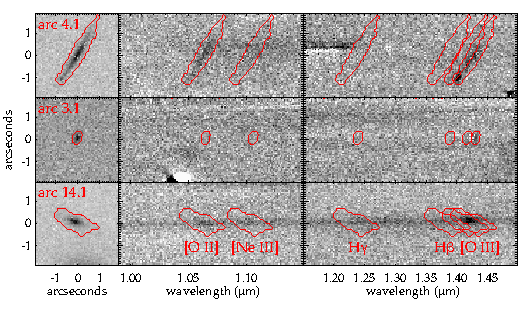
\includegraphics[width=\textwidth]{figures/figure_arcs_spectra_v2.pdf}
    \caption[Grism spectra for the arcs of interest show multiple spatially extended emission lines.]{Grism spectra for the arcs of interest show multiple spatially extended emission
    lines which can be used to derive metallicity maps. From left to right, each row shows the F140W direct
    image, G102 grism spectrum, and G141 grism spectrum. In all cases the estimated contamination has been
    subtracted from the spectra. Strong source continuum is apparent for arc 14.1. Red contours show the object
    segmentation maps derived using the direct images, and mapped to emission lines of interest in the grism
    spectra using the redshift of each source (left to right: \OII $\lambda\lambda$3727, \NeIII $\lambda$3869,
    \Hg, \Hb, \OIII $\lambda$4959, \OIII $\lambda$5007). The redshift is $z=1.855$ for all cases shown here.
    \label{fig:spec2d}}
\end{figure}

\begin{figure}
    \centering
    \includegraphics[width=\textwidth]{figures/figure_arc41_linemaps.pdf}
    \caption[\hst image and emission line maps.]{\hst image (top right; RGB: WFC3/F160W, WFC3/F110W, ACS/F814W) and emission line maps of arc 4.1.
    The typical flux uncertainty in each pixel is $2 \times 10^{-18}$ $\Funit$ (1$\sigma$).
    \label{fig:spec2d_arc4}}
\end{figure}


\section{Gravitational Lensing Model}\label{sec:model}

An accurate gravitational lensing model is essential for reconstructing the source plane morphology of lensed
galaxies, and for combining the information form the multiple images. As one of the Frontier Fields, the
gravitational lensing potential of \clyi\ has been modeled by several groups using a variety of techniques, and
the results are publicly available\footnote{http://www.stsci.edu/hst/campaigns/frontier-fields/}. We compared the
results of all models for which we could derive deflection angle maps at the redshift of interest (those of
Brada{\v c}, CATS, Sharon, and Zitrin) to assess which is best suited to the purposes of this work. We note that
those models are aimed at producing a global description of the cluster and therefore their accuracy in the
vicinity of the lensed images of interest is expected to vary significantly between them. The Sharon version 2
model \citep{Johnson2014} produced the best results for our images, yielding the most precise inversion. The
precision of the inversion was evaluated by comparing for each set of multiple images the promixity of the
inferred source position, and the agreement beetween source plane flux and morphology.  However, even the best
global model produced significant residual differences between the reconstructed sources, requiring an additional
step, as described in the next paragraph.

In order to take full advantage of the multiple images of each arc system, we have developed a novel technique to
align all images in the source plane. This allows us to reduce the lensing-related uncertainties and combine the
data from multiple images to increase signal to noise ratio of the emission line maps. The full details of our
methodology will be presented by Wang et al. (2014, in prep); here we give only a brief overview. Essentially, we
are considering the global cluster model as an approximate first solution and we are seeking corrections to the
potential to improve the reconstruction. We assume that the corrections are small and can thus be described by a
local correction to the lensing potential  up to the first two orders of derivatives.  The first order term
consists of a correction to the deflection angle for each image. The second order term yields corrections to the
shear and convergence. The procedure has thus five free parameters per image. The optimal parameters are found by
requiring the source plane reconstructions of each set of multiple image to be as similar to each other as
possible. We note that a direct byproduct of this formalism is a correction to the magnification of each image.

We have applied this method to the arc systems 3, 4, and 14, using the least distorted (i.e., least magnified)
image of each system as a reference. Table~\ref{tab:magrslt} lists the local convergence and shear before and
after correction, and corrected magnifications. {\bf is this still true?} In all cases the corrected
magnification ratios are in better agreement with measured flux ratios with respect to the original methods. The
morphologies of the reconstructed sources are also in excellent agreement showing that the second order
correction is sufficient for our purposes.

In the following analysis we combine emission line maps from multiple images in the source plane in order to
increase signal to noise ratio. However, including less highly magnified images provides a marginal improvement
at the cost of degraded spatial resolution. We therefore use arcs 3.1$+$3.2, arc 4.1 only, and arcs 14.1$+$14.3
to optimize resolution and sensitivity. Final results are consistent with measurements from individual images.
Combining multiple images improves the precision in metallicity gradients by an impressive factor of
$\simeq2\times$ for arcs 3 and 14 by enabling finer spatial sampling and detection of more extended low surface
brightness emission.

We derive a conservative uncertainty of 13\% RMS in the magnification factors (prior to second order correction)
by comparing measured flux ratios of multiple images with model-predicted magnification ratios. This error is not
propagated in the following analysis, however it is small compared to other sources of uncertainty and has no
effect on the results.

\begin{figure}
    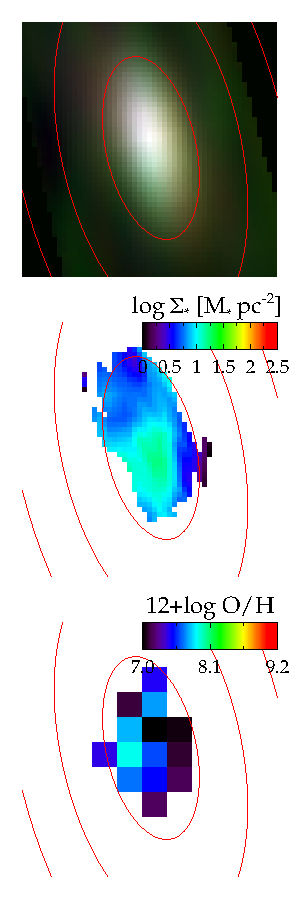
\includegraphics[width=.3\columnwidth]{figures/figure_arc3_source_corr.pdf}
    \hspace{0.03\columnwidth}
    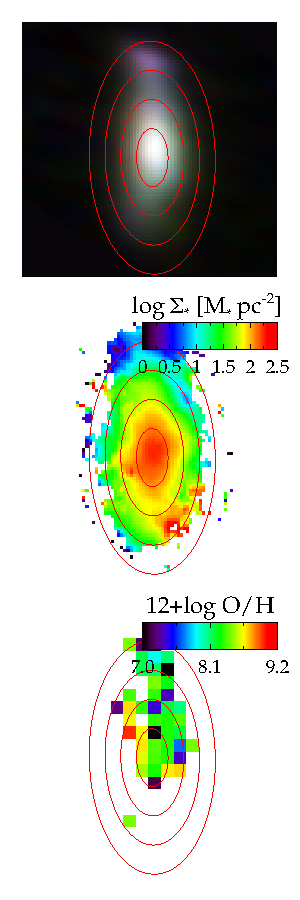
\includegraphics[width=.3\columnwidth]{figures/figure_arc4_source_corr.pdf}
    \hspace{0.03\columnwidth}
    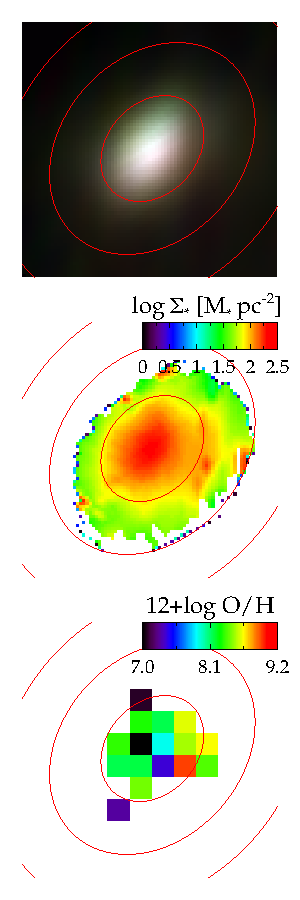
\includegraphics[width=.3\columnwidth]{figures/figure_arc14_source_corr.pdf}
    \caption[Source plane morphologies of arcs 3, 4, and 14.]{
    \label{fig:sourceplane}
    Source plane morphologies of arcs 3, 4, and 14 (from left to right). Each panel shows contours of constant de-projected galactocentric radii at intervals of 1 kpc, derived in Section~\ref{sec:properties}.
    \emph{ Top row:} \hst\ image (RGB: WFC3/F160W, WFC3/F110W, ACS/F814W).
    \emph{ Middle:} stellar mass maps derived from spatially resolved \hst\ photometry. All galaxies have smooth, centrally peaked stellar mass profiles with no significant secondary peaks.
    \emph{ Bottom:} gas-phase metallicity maps.
    }
\end{figure}


\section{Physical Properties}\label{sec:properties}

\subsection{Stellar Mass}\label{sec:mstar}

We use version 1.0 of the stellar population synthesis code FAST \citep{Kriek2009} to fit the resolved spectral
energy density (SED) of each galaxy of interest. For $z=1.855$, the rest-frame UV through optical SEDs are well
constrained by broad-band \hst\ photometry taken as part of the CLASH survey \citep{Postman2012}. We utilize the
ACS/F435W, ACS/F606W, ACS/F814W, and WFC3/F125W filters which sample nearly the full rest-frame wavelength range
from 1250--4900 \AA. This set of filters is chosen to provide the widest possible wavelength coverage while
avoiding contamination from the strong emission lines \lya, \OII, and \OIII which can significantly affect the
broad-band photometry and derived stellar population properties. In particular, \OIII emission accounts for
$\sim$25\% of the total WFC3/F160W flux (an increase of 0.3 magnitudes) for the galaxies discussed here.

Our methodology is as follows. We first align all images with the GLASS F105W direct image and smooth to a common
point spread function of 0\farcs2 FWHM. The broad-band fluxes in each pixel are fit with a \citet{Bruzual2003}
stellar population library, \cite{Chabrier2003} initial mass function, Milky Way dust attenuation law, stellar
ages between 5 Myr and the age of the universe at the galaxy's redshift, and an exponentially declining star
formation history with $\tau = 10^{7}-10^{10}$ yr. The quantity of greatest interest is the derived stellar mass
surface density, which is the most robust parameter. Other stellar population parameters (SFR, age, extinction,
etc.) are obtained simultaneously albeit with larger uncertainty. We have repeated the SED analysis using
additional broad-band filters corrected for emission line contamination using the flux maps described in
Section~\ref{sec:data}, verifying that this produces consistent results. Total stellar masses derived from
integrated photometry and corrected for magnification are listed in Table~\ref{tab:arcs}.


\subsection{Morphology}\label{sec:morphology}

Morphological information is critical for measuring accurate metallicity gradients, as the radial coordinate
depends on a galaxy's central position and inclination. Ideally the dynamical center, major axis orientation, and
inclination would be constrained from kinematics as has been done for previous work \citep[e.g.,][]{Jones2013},
but we lack kinematic data. Instead we derive estimates of these quantities by assuming that the stellar mass
surface density derived in Section~\ref{sec:mstar}, $\Sigma_*$, is elliptically symmetric. We reconstruct
$\Sigma_*$ using the lens model (Section~\ref{sec:model}) and fit for the centroid, orientation, and axis ratio.
Only the most highly magnified image in each arc system is used in order to maximize the spatial resolution. In
the following analysis we adopt the galaxy center and inclination such that contours of $\Sigma_*$ trace contours
of constant de-projected radius.

Source plane $\Sigma_*$ distributions and best-fit ellipses are shown in Figure~\ref{fig:sourceplane}. All
galaxies exhibit smooth, centrally peaked stellar mass profiles with contours that are fit by ellipsoids. Within
the stellar mass uncertainty, we find no evidence for ongoing late-stage major mergers which could manifest as a
secondary peak in the stellar mass density.


\subsection{Metallicity and Nebular Extinction}\label{sec:z}

We use the strong line ratio calibrations presented by \cite{Maiolino2008} to estimate gas-phase oxygen abundance
(expressed as \oh) and nebular extinction A(V) from measured \OII, \NeIII, \Hg, \Hb, and \OIII fluxes. We use a
\cite{Cardelli1989} extinction curve with R$_{\rm V} = 3.1$, noting that the choice of R$_{\rm V}$ has no
significant effect on the derived metallicity (typically $<0.1$ dex for $2\leq {\rm R_V} \leq 5$).  To further
constrain A(V), we impose $\frac{\rm{H}\gamma}{\rm{H}\beta} = 0.47$ as expected for Case B recombination and
typical \HII\ region conditions \citep[e.g.,][]{Hummer1987}.  Metallicity and extinction are derived from a
$\chi^2$ statistic constructed from all available diagnostics: $$\chi^2 = \sum_R \left[ \frac{\Delta
R}{\sigma(R)} \right]^2.$$
%
Here $\Delta R$ is the difference between predicted and observed de-reddened flux ratios at a given A(V) and \oh,
and the uncertainty $\sigma(R)$ includes RMS scatter in each calibration added in quadrature with measurement
uncertainty. We adopt the best fit as the values that minimize $\chi^2$, and 1$\sigma$ uncertainty from the
extrema at which $\chi^2$ differs by 1 from the minimum value. This is slightly smaller than the formal
uncertainty because of covariance between various metallicity diagnostics are independent; we have checked that a
more careful treatment does not affect the results. We limit the solutions to A(V)~$=0-3$ and \oh~$=7.0-9.3$
\citep[equivalent to $0.02-4.1\times$ the solar abundance of \oh~$=8.69$;][]{Allende2001}. While the formal
best-fit solutions are occasionally beyond this range, all such cases are poorly constrained and we view such
extreme conditions as highly unlikely. Although the extinction is poorly constrained for most individual pixels,
SED fitting (Section~\ref{sec:mstar}) and averaged \Hb$/$\Hg\ ratios indicate relatively low extinction toward
both the stars and \HII\ regions, with best-fit A(V)$=0-0.6$ and permitted A(V)$<1.1$ (1$\sigma$) in the dustiest
case. Fortunately, uncertainty in extinction has little effect on the derived metallicity since many diagnostic
line ratios are relatively insensitive to reddening.

Maps of the source plane gas-phase metallicity are shown in Figure~\ref{fig:sourceplane}. The emission line maps
are binned to spatial scales of $\simeq300-500$ pc and the metallicity is fit for all such pixels where at least
one emission line is detected at $\geq 5\sigma$ significance. All sources are well resolved with measurements
extending over $\simeq3$ resolution elements for arc 3, and $\geq 6$ resolution elements for the others. The
metallicity is typically sub-solar with most pixels having best-fit \oh\ in the range 7.5$-$8.5, corresponding to
flux ratios $\frac{\rm [O~\textsc{iii}]}{\rm{H} \beta} > 2.5$ and $\frac{\rm [O~\textsc{iii}]}{\rm
[O~\textsc{ii}]} > 1$. Figure~\ref{fig:sourceplane} also shows several pixels for which the best-fit metallicity
is at the extreme ends of the permitted range; these usually correspond to noise artifacts and/or single-line
detections and are therefore unreliable.

In addition to the spatially resolved analysis, we calculate galaxy-averaged metallicity and extinction by
applying the same analysis to total emission line fluxes measured from integrated 1-D spectra. The results agree
with the average of individual pixel values (Table~\ref{tab:arcs}), providing a valuable sanity check. The
slightly lower average metallicity of individual pixels c.f. integrated flux is likely due to the requirement of
a 5$\sigma$ detection of \OIII (the brightest emission line), which induces a bias toward lower metallicity.
Extinction-corrected Balmer line fluxes derived from this analysis are used to determine star formation rates in
Section~\ref{sec:sfr}.


\subsection{Metallicity Gradient}\label{sec:gradients}

Gas-phase metallicity gradients are derived from the morphology and metallicity analyses described in
Sections~\ref{sec:morphology} and \ref{sec:z}, respectively. We consider two measurements based on (1) individual
pixels and (2) radial binning. For the first method, we compute the gradient $\frac{\Delta Z}{\Delta R}$ from a
linear fit to the metallicity vs. de-projected radius of individual pixels (those shown in
Figure~\ref{fig:sourceplane}):
\begin{equation}\label{eq:gradient} 
    \oh = Z_0 + \frac{\Delta Z}{\Delta R} R.
\end{equation}
This functional form is a good fit to the data and we are unable to distinguish more complex
behavior given the measurement uncertainties. Pixels for which the allowed (1$\sigma$) range of \oh\ extends to
$\leq7$ or $\geq9.3$ are excluded from the fit as these are generally unreliable and have large uncertainty
($\gtrsim 1$ dex), although including these data gives consistent results. For the second method we bin the
emission line flux in annular apertures for each source, calculate metallicity from the total flux in each
aperture, and compute the gradient using Equation~\ref{eq:gradient}. The range of radii for each annulus is
chosen to provide a $\simeq10\sigma$ detection of \OIII, which is uniformly the strongest emission line. We show
the data and best-fit gradients in Figure~\ref{fig:gradients} and list the results in Table~\ref{tab:arcs}.
Uncertainty in inclination and magnification are not included in these error estimates, but these effects are
small ($\lesssim 30$\% combined) compared to uncertainty in the metallicities.

Both methods of calculating the metallicity gradient use the same diagnostics applied to the same data set and
give consistent results. The pixelated approach is similar to local galaxy measurements which are based on
individual \HII\ regions \citep[e.g.,][]{Vila-Costas1992}, and the radial binning method is equivalent to most
measurements reported for high redshift galaxies \citep{Yuan2011,Swinbank2012,Queyrel2012,Stott2014}. The primary
differences are that the annular binning method is higher signal to noise ratio and is spatially complete,
whereas low surface brightness regions are either noisy or excluded from the pixelated method. We therefore
consider the annular binning method to be more robust.


\begin{figure}
    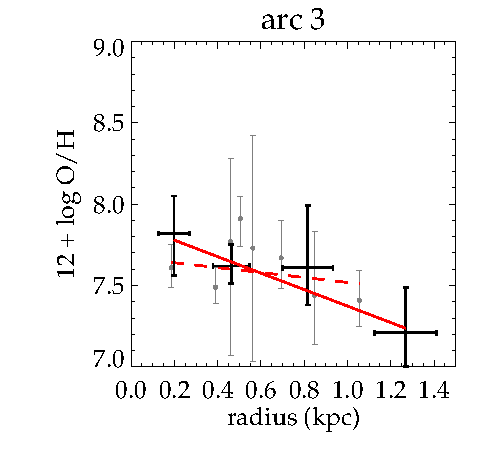
\includegraphics[width=.33\textwidth]{figures/figure_arc3_gradient_bin_corr.pdf}
    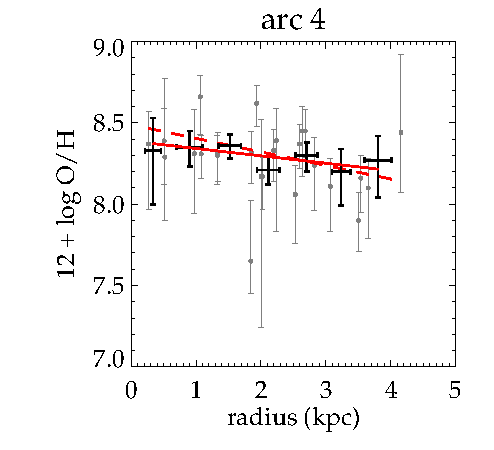
\includegraphics[width=.33\textwidth]{figures/figure_arc4_gradient_bin_corr.pdf}
    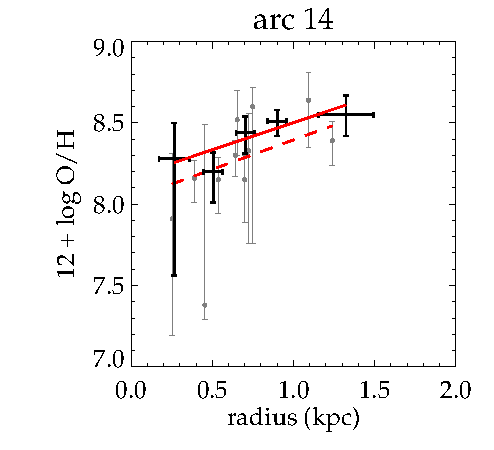
\includegraphics[width=.33\textwidth]{figures/figure_arc14_gradient_bin_corr.pdf}
    \caption[Radial metallicity gradients in each galaxy.]{ \label{fig:gradients} Radial metallicity gradients in each galaxy. Grey points are measured from
    individual source plane pixels shown in Figure~\ref{fig:sourceplane}, and thick black points show the results
    for flux summed within radial annuli. Linear gradient fits to the individual pixels and radial bins are shown
    as dashed and solid lines, respectively. Both methods give consistent results.}
\end{figure}



\subsection{Star Formation Rate}\label{sec:sfr}

Star formation rates are derived from Balmer emission using standard methods. We convert the extinction-corrected
total \Hb flux (Section~\ref{sec:z}) to SFR following \cite{Kennicutt1998}, divide by 1.7 to convert to a
\cite{Chabrier2003} IMF, and divide by the lensing magnification to recover the intrinsic SFR of each galaxy.
Results are given in Table~\ref{tab:arcs} including uncertainty from measurement noise and extinction. Additional
uncertainties associated with the choice of $R_V$ and underlying stellar absorption (for which we make no
correction) are negligible.


\subsection{AGN Contamination}

In calculating metallicities and SFR we have assumed that all nebular emission arises in \HII\ regions. The
presence of shocks or AGN can bias these results even for very weak nuclear sources and we therefore check for
any possible contamination. The global flux ratios of each galaxy, as well as the individual annular bins shown
in Figure~\ref{fig:gradients}, are consistent with \HII\ regions. However in all cases the line ratios fall in
the region occupied by both \HII\ and AGN excitation \citep[such as the "blue" diagnostic diagram,
e.g.,][]{Lamareille2010}, and we lack a low-excitation line such as \NII or \SII which would permit more
reliable classification \citep[e.g.,][]{Jones2013}. Publicly available Chandra/ACIS data\footnote{Available at
http://cxc.cfa.harvard.edu/cda/} show no X-ray detection for any of the arcs, and all three arcs have
moderate-resolution Keck spectra which show no sign of AGN features \citep{Schmidt2014,Limousin2012}. We note
that the central resolution element of arc 14 shows marginal evidence ($\sim2\sigma$) of an elevated \OIII$/$\Hb
ratio as expected for AGN \citep[e.g.,][]{Wright2010,Newman2014}.  \cite{Trump2011} have associated this signal
with a significant AGN fraction in stacks of galaxies of similar stellar mass and redshift whose individual X-ray
luminosities are below the detection threshold, although it is not a reliable indicator of AGN in individual
galaxies.  To summarize, we find no conclusive evidence of AGN but cannot rule out a possible low-level
contribution to the emission line flux from a nuclear source. The expected effect of such activity would be to
lower the derived central metallicity, with no significant effect on SFR or stellar masses.

%= = = = = = = = = = = = = = = = = = = = = = = = = = = = = = = = = = = = = = = =

\begin{deluxetable}{lcccccccc}
\tablecolumns{8}
\tablewidth{0pt}
\tablecaption{Source properties\label{tab:arcs}}

\tablehead{
\colhead{ID} & \colhead{$z$} & \colhead{log M$_*$}      & \colhead{SFR}          & \colhead{\oh\tablenotemark{1}} & \colhead{\oh\tablenotemark{2}} & \colhead{$\Delta \rm{Z} / \Delta \rm{R}$\tablenotemark{3}} & \colhead{$\Delta \rm{Z} / \Delta \rm{R}$\tablenotemark{4}} \\
\colhead{}   & \colhead{}    & \colhead{[log $\Msun$]}  & \colhead{[$\Msunyr$]}  & \colhead{}                 & \colhead{}                       & \colhead{[dex kpc$^{-1}$]}      & \colhead{[dex kpc$^{-1}$]} \\
}
\medskip
\startdata
arc 3   &  1.855  &  7.2$\pm$0.4          &  1.6$^{+1.0}_{-0.6}$  &  7.50$\pm$0.28  &  7.76$^{+0.25}_{-0.20}$  &  -0.15$\pm$0.23  &  -0.51$^{+0.36}_{-0.27}$  \\
arc 4   &  1.855  &  9.3$^{+0.2}_{-0.1}$  &  14.8$^{+21.3}_{-4.3}$  &  8.22$\pm$0.32  &  8.32$^{+0.12}_{-0.15}$  &  -0.08$\pm$0.04  &  -0.05$\pm$0.05  \\
arc 14  &  1.855  &  8.8$^{+0.2}_{-0.1}$  &  3.3$^{+3.2}_{-0.9}$  &  8.21$\pm$0.44  &  8.30$^{+0.15}_{-0.23}$  &   0.36$\pm$0.46  &   0.33$\pm$0.21  \\
\enddata
\tablenotetext{1}{Average and RMS scatter of individual pixels}
\tablenotetext{2}{Best fit and 1$\sigma$ uncertainty derived from integrated spectrum}
\tablenotetext{3}{Derived from individual pixels}
\tablenotetext{4}{Derived from total flux in radial apertures}
\end{deluxetable}


%= = = = = = = = = = = = = = = = = = = = = = = = = = = = = = = = = = = = = = = =


\section{Results and Discussion}\label{sec:results}

\subsection{Global Properties}

In this section we examine the GLASS sample studied here in the context of the general $z\simeq1.8$ galaxy
population, as a prelude to discussing the implications of our results for galaxy evolution.
Figure~\ref{fig:properties} summarizes the demographic properties compared to larger published samples at similar
redshift. Comparison samples are carefully chosen to minimize systematic effects: the narrow range of redshift
mitigates any evolutionary trends, all data points are calculated with the same IMF and stellar population
templates, and all stellar masses account for the contribution of emission lines to broad-band photometry.
Ignoring this last effect would result in higher stellar masses by $\simeq0.15$ dex for arcs 4 and 14 and
$\simeq0.6$ dex for arc 3, in excellent agreement with the mass-dependent estimates by \cite{Whitaker2014}. In
lieu of metallicity, we use \OIII$/$\OII flux ratios for a clear comparison of observable properties. While this
ratio is sensitive to metallicity, ionization parameter, and reddening, all of these quantities are intrinsically
correlated and vary monotonically with \OIII$/$\OII \citep[e.g.,][]{Maiolino2008,Dopita2013}. We can therefore
directly compare {\em relative} oxygen abundances between different samples, noting that secondary parameter
dependences result in $\simeq0.25$ dex RMS scatter between metallicity and \OIII$/$\OII.

In comparison to the overall population, the galaxies studied here have SFRs which are a factor of $\geq3\times$
above the "main sequence" locus of SFR and M$_*$ (Figure~\ref{fig:properties}). Such high relative SFRs are often
induced by gravitational interactions, and indeed \cite{Stott2013} show that $\sim50$\% of sources at this SFR,
M$_*$, and $z$ are merger events. The metallicities inferred from \OIII$/$\OII are consistent with comparison
samples of similar SFR and M$_*$, as are the nebular extinction values. The GLASS data are also consistent with a
steep mass-metallicity relation as found by \cite{Henry2013}, although the scatter in Figure~\ref{fig:properties}
is large. To summarize, the global properties are typical of low-mass starbursts at $z\simeq2$ which are
frequently associated with galaxy interactions.


\begin{figure}
    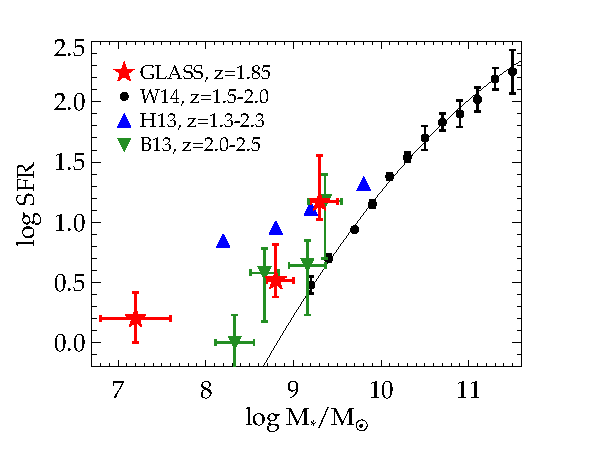
\includegraphics[width=.5\textwidth]{figures/figure_ms_corr.pdf}
    \includegraphics[width=.5\textwidth]{figures/figure_o32_corr.pdf}
    \caption[Global demographic properties of the GLASS arcs.]{Global demographic properties of the GLASS arcs. For comparison we also show average values of
    larger samples at similar redshift from WISP \citep[][H13]{Henry2013} and 3D-HST \citep[][W14]{Whitaker2014}
    data as well as individual lensed galaxies reported by \citet[][B13]{Belli2013}. \emph{ Top:} SFR versus
    stellar mass.  The arcs studied here have significantly higher specific SFR compared to the "main sequence"
    at $z\simeq1.8$ (shown by the W14 data), consistent with expectations for excess star formation triggered by
    gravitational interactions among these systems. \emph{ Bottom:} comparison of emission line ratios versus
    stellar mass. Open symbols show the effect of dust attenuation measured by \cite{Henry2013}; all other data
    are uncorrected for reddening. The arcs studied here have typical \OIII/\OII ratios for their redshift,
    stellar mass, and SFR. The right axis shows equivalent metallicity corresponding to \OIII/\OII for the
    \cite{Maiolino2008} calibration used in this work. The GLASS data are consistent with a steep
    mass-metallicity relation as found by \cite{Henry2013}, and notably extend to an order of magnitude lower in
    stellar mass compared to previous studies at $z\simeq2$.\label{fig:properties}}
\end{figure}


\subsection{Metallicity Gradient Evolution}

We now turn to a discussion of the metallicity gradient of arc 4 and its evolution with redshift.
Figure~\ref{fig:evolution} compares the GLASS data with similar measurements as a function of redshift. Arcs 3
and 14 are not included because their gradients are poorly constrained, due to their small physical sizes and
lower signal to noise ratio.  We restrict the comparison sample to measurements with $\lesssim1$ kpc resolution,
noting that even kpc resolution results in artificially flat inferred gradients for typical high redshift
galaxies \citep[e.g.,][]{Yuan2013,Stott2014}. We show original published values for all comparison data with the
caveat that they are derived using different strong-line calibrations; this has minimal effect on our conclusions
since metallicity gradients are relatively insensitive to the choice of calibration \citep{Jones2013}. However
none of the comparison data include scatter in metallicity in the formal uncertainty, hence the error bar on arc
4 is the most conservative of those shown in Figure~\ref{fig:evolution}.  Ideally we would construct a sample
which corresponds to approximately the same galaxy population \citep[as was done in][]{Jones2013}, but we are
presently limited by the available data at high redshift. The result is that arc 4 is expected to have $\sim0.4$
dex lower stellar masses at a given redshift than average sources in Figure~\ref{fig:evolution}, which are
approximately Milky Way analogs \citep[based on abundance matching; e.g.,][]{Behroozi2013}. Nonetheless this
provides a useful comparison.

Figure~\ref{fig:evolution} demonstrates that interacting galaxies (shown as open symbols) have flatter gradients
than isolated counterparts. This is most evident in the lensed and $z=0$ samples which have the best spatial
resolution. Here we include arc 4 as an interacting system. This is motivated by results which show dramatically
flattened gradients even in widely separated pairs (such as arcs 4--14) compared to an isolated control sample
\citep[][and references therein]{Rich2012}, as well as the enhanced SFR which suggest interaction-driven gas
flows. The relatively shallow metallicity gradient of arc 4 is therefore fully consistent with expected
gravitational interaction.

An alternative cause for the shallow gradient of arc 4 is metal mixing by strong feedback. To illustrate this,
Figure~\ref{fig:evolution} shows evolutionary tracks for two simulations with different sub-grid feedback
prescriptions of an otherwise identical Milky Way-like galaxy discussed by \cite{Gibson2013}, and we now briefly
summarize their findings. The "normal" feedback simulation \citep[MUGS;][]{Stinson2010} results in relatively
steep metallicity gradients of 0.2--0.3 dex\,kpc$^{-1}$ at $z\simeq2$ which flatten at later times. The MaGICC
simulation \citep{Brook2011} employs an enhanced feedback scheme, in which galactic outflows are more effective
at removing metal-enriched ISM material which is re-accreted preferentially in outer regions. This mixing of the
ISM results in shallower gradients of $<0.05$ dex\,kpc$^{-1}$ which become marginally steeper with time. The
enhanced feedback results are in excellent agreement with the shallow gradient measured for arc 4. Other groups
have found essentially identical results with various feedback mechanisms which act to redistribute energy and
ISM material throughout galactic disks \citep[e.g.,][]{Yang2012,Angles-Alcazar2014}. For the case of rapidly
recycled outflows we would expect a signature of higher overall metallicity, whereas gravitational interactions
should have an opposite effect \citep[e.g.,][]{Rich2012}. We note that \cite{Kulas2013} report evidence for rapid
recycling in a protocluster at $z=2.3$ based on stacked spectra, and we might expect a similar observational
signature in the overdense region studied here. However, the expected differences are small \citep[$\sim0.1$
dex;][]{Torrey2012,Kulas2013} compared to measurement uncertainties so we are unable to distinguish these
scenarios without additional complementary data. In any case the shallow gradient in arc 4 suggests that metals
are efficiently mixed throughout the ISM on scales of several kpc.


\begin{figure}
    \centering
    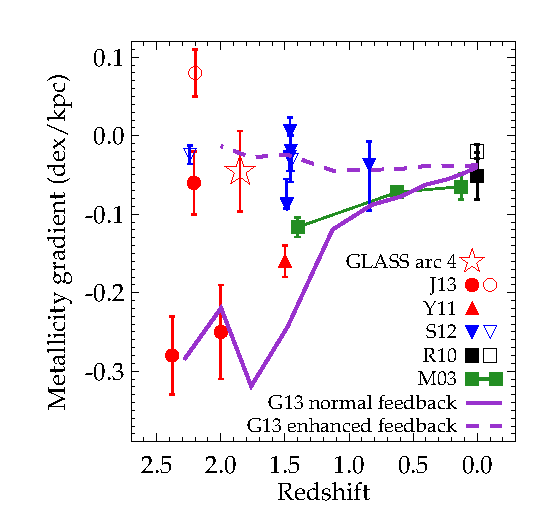
\includegraphics[width=.8\textwidth]{figures/figure_gradient_evolution_corr.pdf}
    \caption[Evolution of metallicity gradients with redshift.]{Evolution of metallicity gradients with redshift. We compare the gradient of arc 4 from this work
    with published measurements at high redshift including other lensed galaxies (\citealt{Jones2013}, J13;
    \citealt{Yuan2011}, Y11), non-lensed galaxies observed with adaptive optics \citep[][S12]{Swinbank2012}, an
    average of local gradients reported by \citet[][R10]{Rupke2010b}, and the Milky Way's metallicity gradient
    evolution measured from planetary nebulae \citep[][M03]{Maciel2003}. Solid and hollow symbols denote isolated
    disks and interacting (or merging) galaxies, respectively, to show that interacting galaxies have flatter
    gradients (closer to zero) on average in the lensed and $z=0$ samples. We additionally show results of two
    different feedback schemes in otherwise identical simulations, described in \cite[][G13; the galaxy shown is
    g15784]{Gibson2013}. The standard feedback results are similar to the Milky Way and isolated lensed galaxies,
    while enhanced feedback leads to shallower gradients at high redshifts and is good agreement with the
    measurement of arc 4 in this work.  \label{fig:evolution}}
\end{figure}


\subsection{A Starbursting Dwarf Galaxy at $z\simeq2$}

One of the most striking aspects of Figure~\ref{fig:properties} is the low stellar mass of arc 3, M$_* = 1.5
\times 10^7 \Msun$. This is an order of magnitude below previous metallicity studies at $z\simeq2$ and extends
into the regime of Milky Way dwarf satellites. Since such galaxies have rarely been studied directly at high
redshift \citep{Christensen2012,Stark2014,Atek2014}, we briefly consider the properties of arc 3 in the context
of recent cosmological simulations and local group analogs.

Both simulations and observations of nearby dwarf galaxies suggest that in the mass regime of arc 3, $\sim$50\%
of its present-day stellar mass has already formed by $z=1.85$ \citep{Shen2014,Weisz2011}. In terms of mass it is
therefore roughly analogous to the "Doc" simulation of \cite{Shen2014}, and to the Milky Way dwarf spheroidal
Fornax \citep[e.g.,][]{Coleman2008}. This is supported by the overall oxygen abundance \oh\,$=7.76$ (equivalent
to [O/H]~$=-0.93$) which is in excellent agreement with the stellar $\alpha$-element abundance distribution of
Fornax \citep{Kirby2011}. Figure~\ref{fig:gradients} indicates a gas-phase metallicity gradient of
$-0.51^{+0.36}_{-0.27}$ which is also in excellent agreement with Fornax's {\em present-day stellar} metallicity
gradient \citep[$-0.50\pm0.10$ dex\,kpc$^{-1}$;][]{Hendricks2014}. However the uncertainty is large, and these
two quantities need not be identical if there is significant radial growth or dynamical evolution of stellar
orbits. Such a steep gradient would imply that the dynamical interaction in arc 3 is insufficient for strong
radial mixing, and this is consistent with \cite{Rich2012} given that the nearest detected neighbor (arc 14) is
separated by 150 kpc in projection.

We measure an instantaneous specific star formation rate of $\log{\rm SSFR (yr^{-1})} = -7.0 \pm 0.5$ for arc 3,
i.e., a mass doubling time of only $10^{7\pm0.5}$ yr. However we caution that this is calculated assuming
constant SFR over the previous $\sim20$ Myr, which is likely not the case: such a high value, as well as the high
ratio of Balmer line flux to UV luminosity and the stellar population modeling described in
Section~\ref{sec:mstar}, suggests a short duty cycle for the current burst of star formation.  Such intense short
starbursts are predicted by several simulations of dwarf galaxies
\citep[e.g.,][]{Governato2012,Zolotov2012,Brooks2014,Shen2014}, and may be triggered by interactions or by
gradual accumulation of a large gas reservoir. Bursty star formation histories are of particular interest in
light of observations that the central regions of local group dwarf galaxies are less dense than predicted for
$\Lambda$CDM cosmology in the absence of baryonic feedback \citep[the "too big to fail"
problem;][]{Boylan-Kolchin2011}. These simulations have found that repeated bursts of star formation and strong
feedback in dwarf galaxies can affect the gravitational potential, transforming dark matter density profiles from
cusps to cores, and have been postulated to reconcile $\Lambda$CDM with observations of local group substructure
\citep[although see also][]{Garrison-Kimmel2013}.  The high SFR surface density of arc 3 is sufficient to drive
outflows with high mass loading factors \citep{Newman2012} as required by these simulations. However we do not
directly constrain the outflow properties, and direct measurements of outflowing gas are extremely challenging
for the luminosity of arc 3. One means of making progress is to measure the mass-metallicity relation slope which
is sensitive to the properties of stellar feedback. The data shown in Figure~\ref{fig:properties} are consistent
with feedback in the form of strong energy-driven galactic winds \citep{Henry2013}, but of course a larger sample
will be required to better constrain the mass-metallicity relation at M$_*\lesssim10^8 \Msun$. We expect several
dozen such sources in the full GLASS survey, which will represent the first statistical constraint of chemical
enrichment and feedback at high redshift in the mass regime where galaxies are in tension with $\Lambda$CDM. The
present data for arc 3 are fully consistent with simulations in which bursty star formation and strong feedback
significantly lower the central density of dwarf galaxies.


\section{Conclusions}\label{sec:conclusions}

This work presents a case study of galaxy evolution in a dense environment at $z=1.85$ from the GLASS survey,
utilizing the spatial resolution of \hst\ aided by gravitational lensing. We study three galaxies in close
physical proximity (50--200 kpc projected separations) and measure their spatially resolved metallicities from
\hst\ grism spectra. Our main results are as follows:
\begin{itemize}
    \item All three galaxies appear to be affected by interaction-induced gas flows, evidenced by their close proximity and specific star formation rates which are $\geq3\times$ above the median value for their M$_*$ and redshift.
    \item We measure a precise metallicity gradient for one galaxy and find a shallow slope compared to other sources at similar redshift, as expected from gravitational interactions. The gradient is also consistent with strong stellar feedback resulting in higher metallicity of accreted (recycled) gas, although we find no evidence of enhanced metallicity which should result from this effect.
    \item The stellar mass range extends an order of magnitude below previous metallicity surveys at $z\simeq2$. The data are consistent with a steep mass-metallicity relation found in previous work, and the full GLASS survey should yield a sufficient sample to measure metallicity trends in the range M$_* \simeq10^7-10^8 \Msun$.
    \item We present the first spatially resolved spectrophotometric analysis of a bona-fide dwarf galaxy at $z\simeq2$ with stellar mass M$_*=10^{7.2\pm0.4}\, \Msun$. It is analogous to Fornax in terms of its stellar mass, metallicity, and metallicity gradient. Its extremely high SSFR indicates a violent starburst, likely with a low duty cycle, consistent with the hypothesis that successive starbursts with strong feedback are responsible for flattening the central density profiles of dwarf galaxies.
\end{itemize}

Measuring accurate metallicity gradients at high redshift is a significant observational challenge which, when
overcome, is expected to elucidate various aspects of the galaxy formation process. Observing lensed galaxies at
$\lesssim0\farcs2$ resolution is the best way to obtain the requisite spatial sampling \citep{Yuan2013}.
Previously only 5 such measurements have been reported in the literature \citep{Jones2010,Jones2013,Yuan2011},
although we note that improvements to the Keck/OSIRIS spectrograph and adaptive optics system have enabled recent
observations of a significantly larger sample (Leethochawalit et al. in prep). Our analysis of \hst\ data
provides further support for a scenario in which gravitational interactions and mergers cause a temporary
flattening of gradients, while isolated galaxies at high redshift have steep negative metallicity gradients
consistent with standard feedback models. More importantly, our results constitute a proof-of-concept that \hst\
grism spectra obtained with the GLASS survey yield precise gradient slope measurements with conservative
uncertainty $\simeq0.05$ dex\,kpc$^{-1}$ in good cases. This is enabled by the combination of broad wavelength
coverage and high spatial resolution aided by gravitational lensing. This paper presents the complete methodology
developed for such measurements, including a significant improvement over previous lensing studies by combining
data from multiple strongly lensed images (Section~\ref{sec:model}; Wang et al. in prep). Based on current data
we expect the GLASS survey to yield high-quality gradient measurements (comparable to arc 4) for approximately 20
galaxies. We anticipate that such a large sample will conclusively establish whether metallicity gradient slopes
are steeper or shallower at $z\simeq2$ compared to local descendants, and more generally how metallicity
gradients evolve over time. This will have significant implications for sub-grid feedback prescriptions used in
cosmological simulations \citep[e.g.,][]{Gibson2013,Angles-Alcazar2014}, which in turn inform our understanding
of baryon cycling and chemical enrichment of the circum- and inter-galactic media, and the role of this baryon
cycle in galaxy formation.




\chapter{Sub-kiloparsec Resolution Gas-phase Metallicity Maps at Cosmic Noon behind the Hubble Frontier Fields
cluster \clyi}

\section{Introduction}\label{sect:intro}

Galaxies are complex ecosystems, particularly at the peak epoch of cosmic star formation,
corresponding to the redshift range of $z$$\sim$1-3, also known as the ``cosmic noon''
\citep[see][for a recent review]{2014ARA&A..52..415M}.  During this approximately 4 Gyr, the
Hubble sequence gradually breaks down and the predominant morphology of galaxies transforms
from irregular systems at high redshifts to symmetric disks and bulges at low redshifts
\citep{Mortlock:2013dg}.  This complexity is to a large extent induced by the interplay
between the process of star formation, and the diverse aspects of baryonic cycling, \eg,
galactic feedback, gas inflows/outflows, and major/minor mergers
\citep{2011MNRAS.415...11D,Martin:2012dx}.  The effect of environment surrounding galaxies
can further complicate the spatial distribution of star formation, as recently revealed by
\citet{2015ApJ...814..161V,TheGrismlensampli:-R7Qg0z6}.
Measurements of gas-phase metallicity, \ie, the chemical abundances of elements heavier than
hydrogen and helium in the interstellar medium (ISM), are a powerful means to shed light on
this complexity,
because the metal enrichment history is strongly tied to the mass assembly history in galaxy evolution
\citep{2011MNRAS.416.1354D,Lu:2015ic}.  Since detailed elemental abundances are not directly measurable at extragalactic
distances, the relative oxygen abundance in ionized gaseous nebulae, \ie, \oh, is often chosen as the observational proxy of
metallicity.

For over a decade, a tight correlation between metallicity and galaxy stellar mass (\Mstar),
\ie, the mass-metallicity relation (MZR), has been quantitatively established, from the vast
database of local galaxies observed by the Sloan Digital Sky Survey
\citep{Tremonti:2004ed,Zahid:2012fp,Andrews:2013dn}. This relation has been further extended to high redshifts, using
deep near infrared (IR) spectroscopy facilitated by large ground-based and space-based
telescopes \citep{Erb:2006kn,2008A&A...488..463M,Zahid:2011bb,Henry:2013gx,2014ApJ...795..165S,Sanders:2015gk,Guo:2016wk}.
The measurements of the MZR as a function of redshift can cast useful constraints on various galaxy evolution models, since the
slope of the MZR is sensitive to the properties of outflows, such as the mass loading factor and the outflow speed \citep[see,
\eg,][]{2012MNRAS.421...98D,Lu:2015kh}.
This slope can also be explained by variations of star-formation efficiency and gas mass fraction in galaxies with different
stellar masses \citep[see, \eg,][]{Baldry:2008hm,TheUniversalRelati:2014kx}.
The normalization of the MZR can shed light upon the stellar chemical yield across cosmic time \citep{2008MNRAS.385.2181F}.
\citet{2010MNRAS.408.2115M} first suggested that there exists a so-called fundamental metallicity relation (FMR) in
the 3D parameter space spanned by \Mstar, \sfr (SFR), and metallicity, such that the MZR is merely a 2D projection of this more
fundamental 3D manifold \citep[see also][]{Hunt:2016ui}.
This 3D scaling relation shows a tight scatter ($\sim$0.05 dex) in metallicity and is speculated to not evolve with $z$.
In this context, the apparent redshift evolution of the MZR normalization originates primarily from sampling the FMR in terms of
galaxies with different SFR. This concept of the FMR is in accord with the gas regulator model proposed by \citet{Lilly:2013ko}, 
even though mergers can also play a subtle role in shaping the form of the FMR by increasing the scatter 
\citep{MichelDansac:2008gp}. However, at high redshifts, the validity of the FMR is still under investigation \citep[see, 
\eg,][]{Sanders:2015gk,Wuyts:2014ed}.

Spatially resolved chemical information provides a more powerful diagnostic tool about galaxy baryonic assembly than
integrated metallicity measurements, especially at high redshifts. Because for non-interacting galaxies, their metallicity radial 
gradients are found to be highly sensitive to the properties of gas, \ie, the surface density, the existence of inflows/outflows, and the kinematic
structure \citep{Cresci:2010hr,2013ApJ...765...48J,2014A&A...563A..49S,Metallicityevolutio:2014kg}.
In the past few years, metallicity radial gradients, measured from spectroscopic data
acquired by ground-based instruments with natural seeing ($\gtrsim$$0\farcs6$), have been
reported at high redshifts
\citep{Queyrel:2012hw,Metallicityevolutio:2014kg,2014MNRAS.443.2695S}. In particular, a large
mass-selected sample of galaxies at $0.7\lesssim z\lesssim2.7$ were observed with spatially
resolved gas kinematics and star formation, using the K-band Multi Object Spectrograph
(\kmos) on the Very Large Telescope (\vlt) \citep[\ie, the \kd
survey,][]{2015ApJ...799..209W}.  As a result, \citet{Wuyts:2016th} measured \mgs for 180 \sf
galaxies in three redshift intervals (\ie [0.8, 1.0], [1.3, 1.7], and [2.0, 2.6]), and found
that the majority of the \mgs are flat and no statistical significant correlations between
\mgs, and stellar, kinematic, and structural properties of the galaxy.

However, seeing-limited measurements typically have insufficient resolution to resolve the inner structure of galaxies at
$z\gtrsim1$, and the inferred metallicity gradient can be potentially biased. For example, \citet{2013ApJ...767..106Y} showed that
coarse spatial sampling ($\geq$1 \kpc) can result in artificially flat \mgs, inferring that sufficiently high spatial resolution,
\ie, \emph{sub-kpc} scale (corresponding to an angular resolution of $<0\farcs2$-$0\farcs3$), is crucial in yielding precise
information of how metals are distributed spatially in extragalactic \HII regions.  Only a few \mgms meet this requirement,
including a sample of 9 \Ha-selected galaxies at $z\in[0.84,2.23]$ (the majority at $z\sim1.45$), observed with the adaptive
optics (AO) assisted integral field unit (IFU) spectrograph \sinf onboard the \vlt \citep{2012MNRAS.426..935S}. Even higher
resolution can be attained through the combination of diffraction-limited data and gravitational lensing as shown by
\citet{2010ApJ...725L.176J,2013ApJ...765...48J,Yuan:2011hj}, targeting strongly lensed galaxies with the laser guide star AO aided
IFU spectrograph \osiris at the \keck telescope. Following this approach, \citet{2015arXiv150901279L} recently analyzed a sample
of 11 lensed galaxies (3 at $z\sim1.45$ and the rest at $z\gtrsim2$), deriving maps of both metallicity and emission line (EL)
kinematics.  Although a great amount of effort has been invested in enlarging the sample size of high-$z$ \mgs obtained with
sub-kpc scale spatial resolution, the current sample consists of only $\lesssim30$ such gradients and is still statistically
insufficient to explore trends with stellar mass and redshift.

In order to enlarge the sample of sub-kpc resolution measurements, we recently demonstrated that such metallicity maps can be
derived using space-based data \citep{2015AJ....149..107J}. We measured a flat metallicity gradient in a multiply lensed
interacting system at $z=1.85$, using diffraction-limited Hubble Space Telescope (\hst) grism data, and confirmed that flat \mgs 
can be caused by gravitational interactions in merging systems.

The main goal of the work presented here is to collect a uniformly analyzed large sample of high-$z$ metallicity maps obtained
with sub-kpc spatial resolution. To meet our goal, we improve upon the methodology proposed in our pilot paper
\citep{2015AJ....149..107J}, in particular via developing a novel Bayesian method to imply metallicity from multiple EL
diagnostics simultaneously. We apply our advanced analysis to ultra-deep grism data of the massive galaxy cluster \clyi, thus
exploiting the powerful synergy of \hst diffraction-limited spectroscopy and lensing magnification.

The outline of this Chapter is as follows. In Section~\ref{sect:spec}, we introduce the spectroscopic observations used in this work
and the selection of our \mg sample. The photometric data and galaxy cluster lens models are briefed in Section~\ref{sect:phot}.
We then present our entire analysis process in Section~\ref{sect:analysis}, and show our results in terms of global demographics
and spatially resolved analysis in Sections~\ref{sect:global} and \ref{sect:sra}, respectively.  Finally,
Section~\ref{sect:conclu} will conclude and discuss our study. The concordance cosmological model (\Om=0.3, \Ol=0.7,
$H_0=70\Hunit$) and the AB magnitude system \citep{1983ApJ...266..713O} are used throughout.  Without specific number
showing the wavelength, the names of forbidden lines are simplified as $\OII~\lambda\lambda3726,3729\defeq\OII$,
$\OIII~\lambda5008\defeq\OIII$, $\NII~\lambda6585\defeq\NII$, $\SII~\lambda\lambda6718,6732\defeq\SII$\footnote{The
wavelength values are taken from \url{http://classic.sdss.org/dr7/algorithms/linestable.html}}.


\section{Spectroscopic Data and Sample Selection}\label{sect:spec}

In Section~\ref{subsect:hstdata}, we summarize our \hst grism observations, data quality, and data reduction.
Our sample selection criteria are then described in Section~\ref{subsect:srcselect}.
We also carried out some ground-based integral field unit (IFU) observations on part of our sample, which are presented in 
Appendix~\ref{sect:kinem}.
%In Section~\ref{subsect:ifu}, we summarize the ground based kinematic data that we will use to supplement and interpret the
%metallicity and star formation maps obtained from the \hst grism spectroscopy.

\subsection{Hubble Space Telescope Grism Spectroscopy}\label{subsect:hstdata}

%= = = = = = = = = = = = = = = = = = = = = = = = = = = = = = = = = = = = = = = =
% = = = = = = = = = = = = = = = = = = = = = = = = = = = = = = = = = = = = = = = = = =
% Include this table with \input{filename.tex}
% To rotate in emulateapj do: \begin{turnpage}\input{filename.tex}\end{turnpage}
% To display it on multiple pages do: \LongTables\input{filename.tex}
% - - - - - - - - - - - - - - - - - - - - - - - - - - - - - - - - - - - - - - - - - -
\begin{deluxetable}{cccp{4cm}ccccccccc}
    \tablecolumns{13}
    \tabcolsep=0.3cm
    \tablewidth{0pt}
    \tablecaption{Properties of the grism spectroscopic data used in this work}
% - - - - - - - - - - - - - - - - - - - - - - - - - - - - - - - - - - - - - - - - - -
\tablehead{
    \colhead{PA\tablenotemark{a}} &
    \colhead{Grism} &
    \colhead{Exposure Time} &
    \colhead{Program}  &
    \colhead{Time of completion}\\
    \colhead{(deg.)} & & 
    \colhead{(s)} & & &
}
%---------------------------------------------------------------
\startdata
\multirow{2}{*}{032}    & G102 & 8723 & \glass & \multirow{2}{*}{Feburary 2014} \\
                        & G141 & 4412 & \glass  \\
111                     & G141 & 36088 & SN Refsdal follow-up & December 2014 \\
119                     & G141 & 36088 & SN Refsdal follow-up & January 2015 \\
\multirow{2}{*}{125}    & G102 & 8623 & \glass & \multirow{2}{*}{November 2014} \\
                        & G141 & 4412 & \glass
\enddata
% - - - - - - - - - - - - - - - - - - - - - - - - - - - - - - - - - - - - - - - - - -
\tablecomments{Here we only include the grism observations targetted on the prime field of
\clsan.}
\tablenotetext{a}{The position angle shown here corresponds to the ``PA\_V3'' value
    reported in the WFC3/IR image headers. The position angle of the dispersion axis of the
grism spectra is given by $\mathrm{PA_{disp}} \approx \mathrm{PA\_V3} - 45$.}
\label{tab:obsdata}
\end{deluxetable}

%= = = = = = = = = = = = = = = = = = = = = = = = = = = = = = = = = = = = = = = =

\subsubsection{The Grism Lens-Amplified Survey from Space}\label{subsect:glass}

The Grism Lens-Amplified Survey from Space\footnote{\url{http://glass.astro.ucla.edu}} \citep[\glass; Proposal ID 13459;
P.I. Treu,][]{2014ApJ...782L..36S,2015ApJ...812..114T} is an \hst cycle 21 large general observing (GO) program.  \glass
observed 10 massive galaxy
clusters with the Wide Field Camera 3 Infrared (WFC3/IR) grisms (G102 and G141; 10 and 4 orbits per cluster,
respectively) targeted at their centers and the Advanced Camera for Survey (ACS) Optical grism (G800L) at their infall
regions.
The exposure on each cluster core is split into two nearly orthogonal
position angles (PAs), in order to disentangle contamination from neighboring objects.
Data acquisition was completed in January 2015. Here we focus on the grism data targeted on the center of
\clyi taken in February 2014 (PA=$032^{\circ}$) and November 2014 (PA=$125^{\circ}$), marked by blue squares in
Figure~\ref{fig:RGBfullFoV} (also see Table~\ref{tab:obsdata}). \glass provides $\sim$10\% of the G141
exposures used in this work, and 100\% of the G102 exposures.  Details on \glass data reduction can be found in
\citet{2014ApJ...782L..36S,2015ApJ...812..114T}.

\begin{figure}
    \centering
    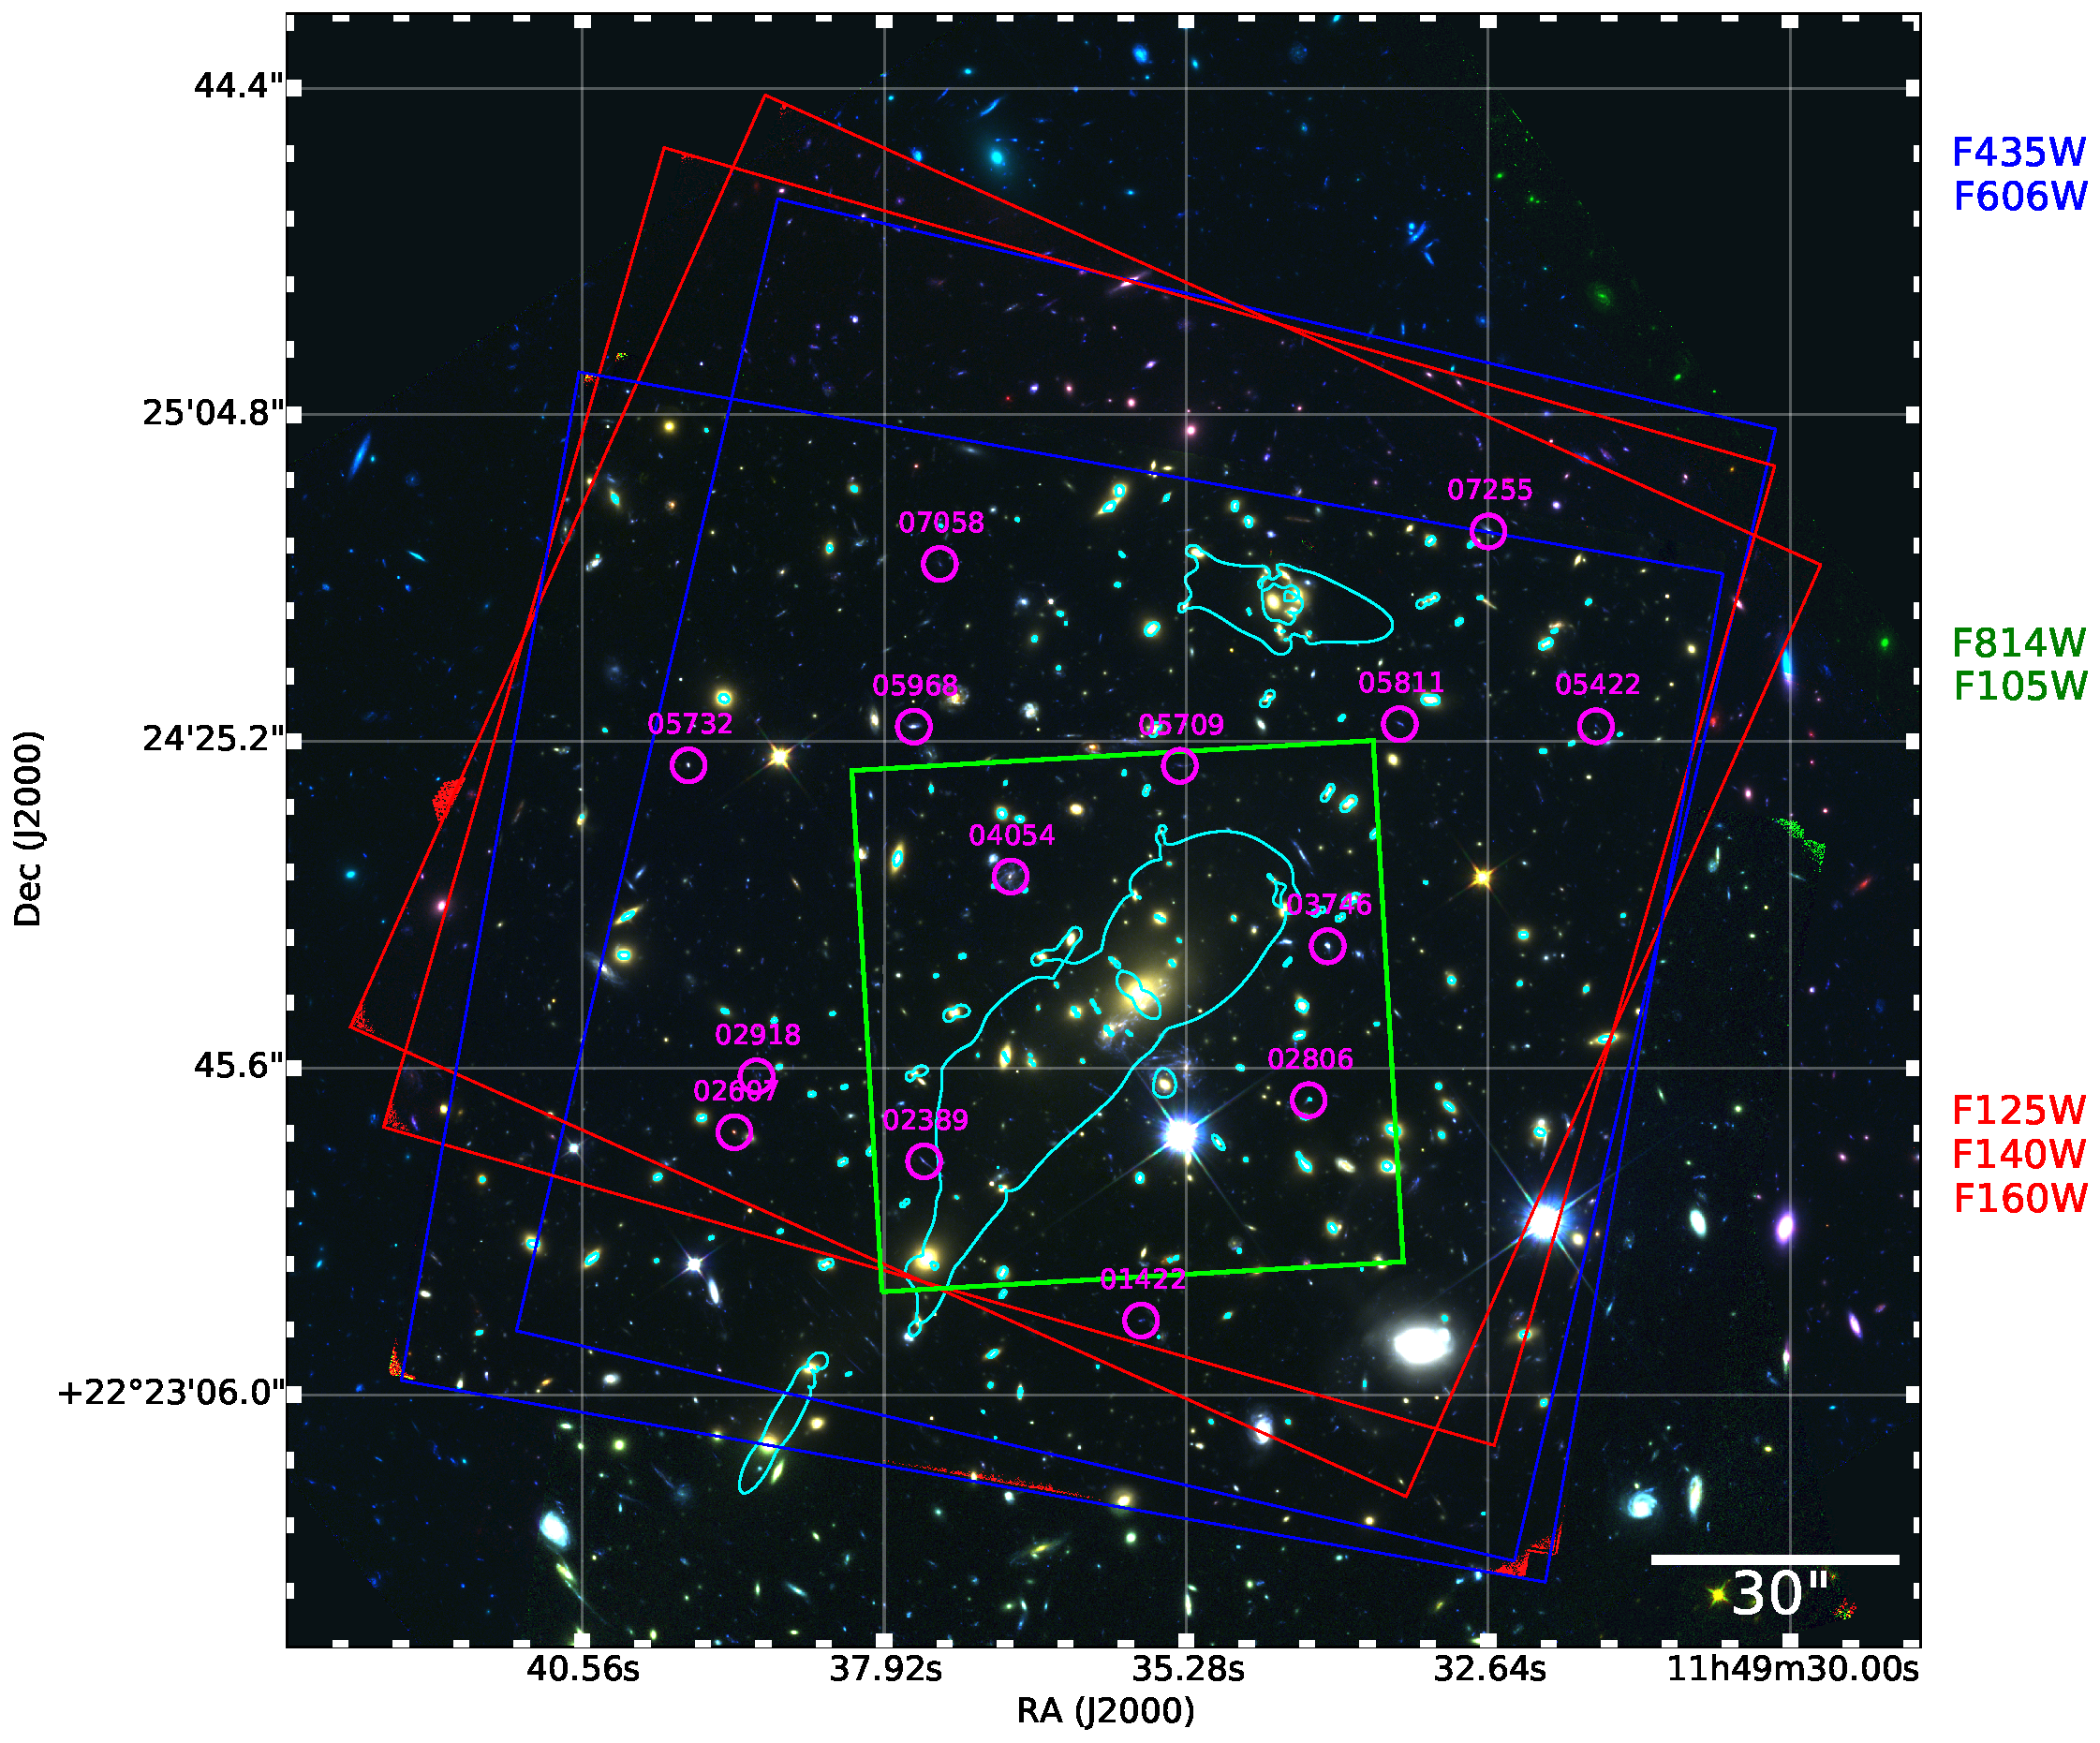
\includegraphics[width=\textwidth]{fig/clM1149_rgb_allfilters_hires.pdf}
    \caption[Color composite image of \clyi from the full-depth 7-filter \hff photometry.]{Color composite image of \clyi from the full-depth 7-filter \hff photometry.
    The blue, green, and red channels are comprised of the \hst broad-band filters shown on
    the right. The blue, red and green squares mark the footprints of \glass, the Refsdal
    follow-up, and \muse programs utilized in this work.  The cyan contours are the critical
    curves at $z=1.8$ predicted by the \glafic version 3 lens model.
    The critical curves denote the regions where lensing magnification reaches infinity.
    Thus the closer proximity between the object and the critical curve at the object's redshift indicates higher magnification
    that the object has.
    The magenta circles show the positions of our \mg sample. 3$\times$3 arcsec$^2$ zoom-in postage stamps around
    these positions are shown in Figure~\ref{fig:RGBstamps}.
    \label{fig:RGBfullFoV}}
\end{figure}

Shallow images through filters F105W or F140W were taken to aid the
alignment and extraction of grism spectra. The imaging exposures are
combined with the exposures obtained by the Hubble Frontier
Fields (\hff) initiative and other programs to produce the deep
stacks, released as part of the \hff program (see Section~\ref{sect:phot}
for more details).

\subsubsection{The Supernova Refsdal Follow-up Program with \protect\hst G141}\label{subsect:refsdal}

The majority of the G141 exposures used in this work (30 orbits) were taken as part of the follow-up \hst GO/DDT
campaign (Proposal ID 14041, P.I. Kelly, Brammer et al. in prep.) of the first multiply
imaged supernova, SN Refsdal \citep{2015Sci...347.1123K}. Two pointings
(shown by the red squares in Figure~\ref{fig:RGBfullFoV}) were exposed between December 2014 and January 2015 with 8 degrees apart
(\ie
at PA=$111^{\circ}$, and $119^{\circ}$ respectively, as shown in Table~\ref{tab:obsdata}), in order to optimize the spectroscopy
of SN Refsdal.  The analysis of the
spectra of SN Refsdal, which showed that it was SN 1987A-like, is described by \citet{2015arXiv151209093K}.

\subsubsection{Grism Data Reduction}

The combined grism dataset was reduced following the procedure of the
3D-\hst survey \citep{Brammer:2012bu,Momcheva:2016fr}. An updated
3D-\hst pipeline \footnote{\url{http://code.google.com/p/threedhst/}}
was employed to reduce the images and spectra. The \adriz software
from the \dpac package and \verb+tweakreg+ were used to align and
combine individual grism exposures, subtracting the sky images
provided by \citet{Brammer:2012bu}. The time-varying sky background
due to helium glow (at 10,830 \AA) in the Earth exosphere was also
accounted for according to \citet{Brammer:2014wl}. After these initial
steps, the mosaics were co-added through interlacing onto a grid of
0\farcs065 resolution, Nyquist sampling the point spread function (PSF)
full width half maximum (FWHM).  The average spectral resolution is $R$$\sim$210
and $R$$\sim$130 for G102 and G141, respectively. The average pixel scale
after interlacing is 12 \AA{} and 22 \AA{} respectively for G102 and G141.

We used the co-added \H-band mosaics as the detection image, on which \sex
was run. An object catalog was generated and a
corresponding segmentation map was created for each object,
determining which spatial pixels (spaxels) belong to this object. Thus for a source
registered in the catalog and falling within the WFC3 grism field-of-view (FoV), we
extracted its spectra from grism mosaics through adding up the
dispersed flux for all spaxels within an area defined by the
segmentation image of this source, after flat-field correction and
background subtraction.  The ``fluxcube'' model from the \axe package
\citep{Kummel:2009dn} was employed to generate the 2D models of stellar
spectrum, based upon the spatial profile of the source, the color
information from direct image mosaics (if available), and the grism
calibration configurations.  For sources of interest, this model
serves as the continuum model which we re-scaled and subtracted from
the observed 2D spectra (see Section~\ref{subsect:combELmaps} for more
details) in order to obtain pure EL maps. At the same time, if the object is a bright contaminating neighbour,
this 2D model also functions as spectral contamination, which is subtracted before the continuum removal.

The data used in this work contain a total of 34 orbits of G141 and 10 orbits of G102,
reaching a 1-$\sigma$ flux limit (uncorrected for lensing magnification) of 3.5(1.2)$\times$$10^{-18}$ \Funit over the wavelength
range of G102(G141), calculated from \citet{Schmidt:2016ez}. Our data provide an uninterrupted wavelength coverage in the range of
0.8-1.7 \micron and make this particular field one of the deepest fields probed by \hst spectroscopy to date.

\subsection{Sample Selection}\label{subsect:srcselect}

\begin{landscape}
%= = = = = = = = = = = = = = = = = = = = = = = = = = = = = = = = = = = = = = = =
% = = = = = = = = = = = = = = = = = = = = = = = = = = = = = = = = = = = = = = = = = =
% Include this table with \input{filename.tex}
% To rotate in emulateapj do: \begin{turnpage}\input{filename.tex}\end{turnpage}
% To display it on multiple pages do: \LongTables\input{filename.tex}
% - - - - - - - - - - - - - - - - - - - - - - - - - - - - - - - - - - - - - - - - - -
%\tabletypesize{\small} 
\tabcolsep=0.1cm
\begin{deluxetable}{ccccccccccccc} \tablecolumns{13}
\tablewidth{0pt}
\tablecaption{Global demographic properties of the \mg sample analyzed in this work}
% - - - - - - - - - - - - - - - - - - - - - - - - - - - - - - - - - - - - - - - - - -
\tablehead{
  \colhead{ID} &
  \colhead{R.A.} &
  \colhead{Dec.} &
  \colhead{$z_{\textrm{spec}}$} &
  \colhead{$\mu$\tablenotemark{a}} &
  \colhead{\H magnitude} &
  \multicolumn{2}{c}{SED fitting} &
  \multicolumn{3}{c}{EL diagnostics} \\
  & [deg.] & [deg.] &  &  & [ABmag] & \multicolumn{2}{c}{\hrulefill} & \multicolumn{3}{c}{\hrulefill} & \\
    & & & & & & log(\Mstar\tablenotemark{b}/\Msun) & $\Av^{\rm S}$\tablenotemark{c} &  \oh  & SFR\tablenotemark{b} [\Msun/yr] &
    $\Av^{\rm N}$\tablenotemark{c}
}
%---------------------------------------------------------------
\startdata
01422  &  177.398643  &  22.387499  &  2.28  &  2.35 [2.09, 2.26]  &  24.46  &  $9.29_{-0.01}^{+0.07}$  &  $<0.01$  &  $8.26_{-0.13}^{+0.11}$  &  $15.10_{-7.11}^{+16.76}$  &  $<1.07$  \\
02389  &  177.406546  &  22.392860  &  1.89  &  43.25 [37.47, 50.28]  &  23.29  &  $8.43_{-0.07}^{+0.06}$  &  $<0.01$  &  $7.88_{-0.15}^{+0.16}$  &  $<6.37$  &  $1.36_{-0.82}^{+0.69}$  \\
02607\tablenotemark{d}  &  177.413454  &  22.393843  &  1.86  &  3.01 [2.79, 2.98]  &  22.63  &  $10.25_{-0.10}^{+0.06}$  &  $1.70_{-0.18}^{+0.42}$  &  $7.70_{-0.11}^{+0.13}$  &  $>36.51$  &  $2.26_{-0.58}^{+0.31}$  \\
02806  &  177.392541  &  22.394921  &  1.50  &  4.82 [3.11, 3.51]  &  23.35  &  $8.72_{-0.01}^{+0.19}$  &  $0.50_{-0.01}^{+0.01}$  &  $7.96_{-0.16}^{+0.15}$  &  $1.96_{-0.13}^{+1.37}$  &  $<0.18$  \\
02918  &  177.412652  &  22.395723  &  1.78  &  2.95 [2.72, 2.91]  &  25.22  &  $8.37_{-0.08}^{+0.15}$  &  $0.10_{-0.10}^{+0.34}$  &  $8.42_{-0.14}^{+0.11}$  &  $<70.32$  &  $1.25_{-0.80}^{+0.72}$  \\
03746  &  177.391848  &  22.400105  &  1.25  &  3.78 [3.56, 3.83]  &  22.48  &  $8.81_{-0.01}^{+0.03}$  &  $<0.01$  &  $8.11_{-0.11}^{+0.10}$  &  $10.95_{-0.58}^{+1.61}$  &  $<0.17$  \\
04054  &  177.403393  &  22.402456  &  1.49  &  3.39 [3.04, 3.28]  &  21.27  &  $9.64_{-0.01}^{+0.05}$  &  $1.10_{-0.01}^{+0.01}$  &  $8.70_{-0.11}^{+0.09}$  &  $16.99_{-2.80}^{+5.71}$  &  $0.72_{-0.23}^{+0.23}$  \\
05422  &  177.382077  &  22.407510  &  1.97  &  3.63 [3.11, 4.41]  &  25.05  &  $8.45_{-0.46}^{+0.15}$  &  $0.00_{-0.01}^{+0.56}$  &  $7.56_{-0.12}^{+0.16}$  &  $<38.18$  &  $<1.85$  \\
05709  &  177.397234  &  22.406181  &  1.68  &  7.10 [6.74, 7.53]  &  25.44  &  $7.90_{-0.03}^{+0.02}$  &  $<0.01$  &  $8.21_{-0.21}^{+0.13}$  &  $<17.97$  &  $<1.18$  \\
05732  &  177.415126  &  22.406195  &  1.68  &  1.56 [1.51, 1.61]  &  23.45  &  $9.09_{-0.01}^{+0.01}$  &  $<0.01$  &  $8.41_{-0.12}^{+0.10}$  &  $<84.70$  &  $<1.31$  \\
05811  &  177.389220  &  22.407583  &  2.31  &  7.50 [6.88, 9.34]  &  23.79  &  $8.85_{-0.10}^{+0.11}$  &  $<0.01$  &  $8.16_{-0.21}^{+0.14}$  &  $4.94_{-2.47}^{+3.13}$  &  $<0.74$  \\
05968  &  177.406922  &  22.407499  &  1.48  &  1.84 [1.78, 1.96]  &  22.24  &  $9.34_{-0.03}^{+0.02}$  &  $0.60_{-0.01}^{+0.20}$  &  $8.47_{-0.08}^{+0.07}$  &  $27.95_{-4.41}^{+4.70}$  &  $0.23_{-0.13}^{+0.15}$  \\
07058  &  177.405976  &  22.412977  &  1.79  &  2.13 [1.97, 3.01]  &  24.28  &  $8.74_{-0.15}^{+0.17}$  &  $0.00_{-0.01}^{+0.12}$  &  $8.38_{-0.19}^{+0.13}$  &  $<44.99$  &  $<1.85$  \\
07255  &  177.385990  &  22.414074  &  1.27  &  2.34 [2.31, 2.99]  &  22.47  &  $9.36_{-0.21}^{+0.01}$  &  $0.30_{-0.01}^{+0.21}$  &  $8.38_{-0.08}^{+0.08}$  &  $8.73_{-3.10}^{+3.53}$  &  $<0.79$
\enddata
% - - - - - - - - - - - - - - - - - - - - - - - - - - - - - - - - - - - - - - - - - -
\tablecomments{The error bars and upper/lower limits shown in the columns of SED fitting and EL diagnostics correspond
    to 1-$\sigma$ confidence ranges. Note that the errors on the SED fitting results do not include any systematic uncertainties associated with the
    \citet{Bruzual:2003ck} stellar population models.}
\tablenotetext{a}{Best-fit magnification values and 1-$\sigma$ confidence intervals. Except for galaxy ID 02389, the
magnification results are from the \glafic version 3 model, calculated by the \hff interactive online magnification
calculator available at \url{https://archive.stsci.edu/prepds/frontier/lensmodels/webtool/magnif.html}. 
For galaxy ID 02389, we use the \SJ version 3 model instead to compute the magnification results and correct for
lensing magnification}
\tablenotetext{b}{Values presented here are corrected for lensing magnification.}
\tablenotetext{c}{The superscripts of ``S'' and ``N'' refer to the stellar and nebular V-band dust extinction in units of
    magnitude, respectively.}
\tablenotetext{d}{The EL diagnostic result on this source is not trustworthy, since it is classified as an AGN
    candidate (see Sect.~\ref{sect:global}).}
\label{tab:srcprop}
\end{deluxetable}

%= = = = = = = = = = = = = = = = = = = = = = = = = = = = = = = = = = = = = = = =
\end{landscape}

The selection of our \mg sample is based upon the master redshift
catalog for \clyi\footnote{available at \url{https://archive.stsci.edu/prepds/glass/}}, published by the \glass collaboration.
As described by \citet{2015arXiv151005750T}, redshifts were determined by combining
spectroscopic information from \glass and the SN Refsdal follow-up \hst
grism programs, ground-based \muse observations and Keck \deimos data.

\begin{figure}
    \centering
    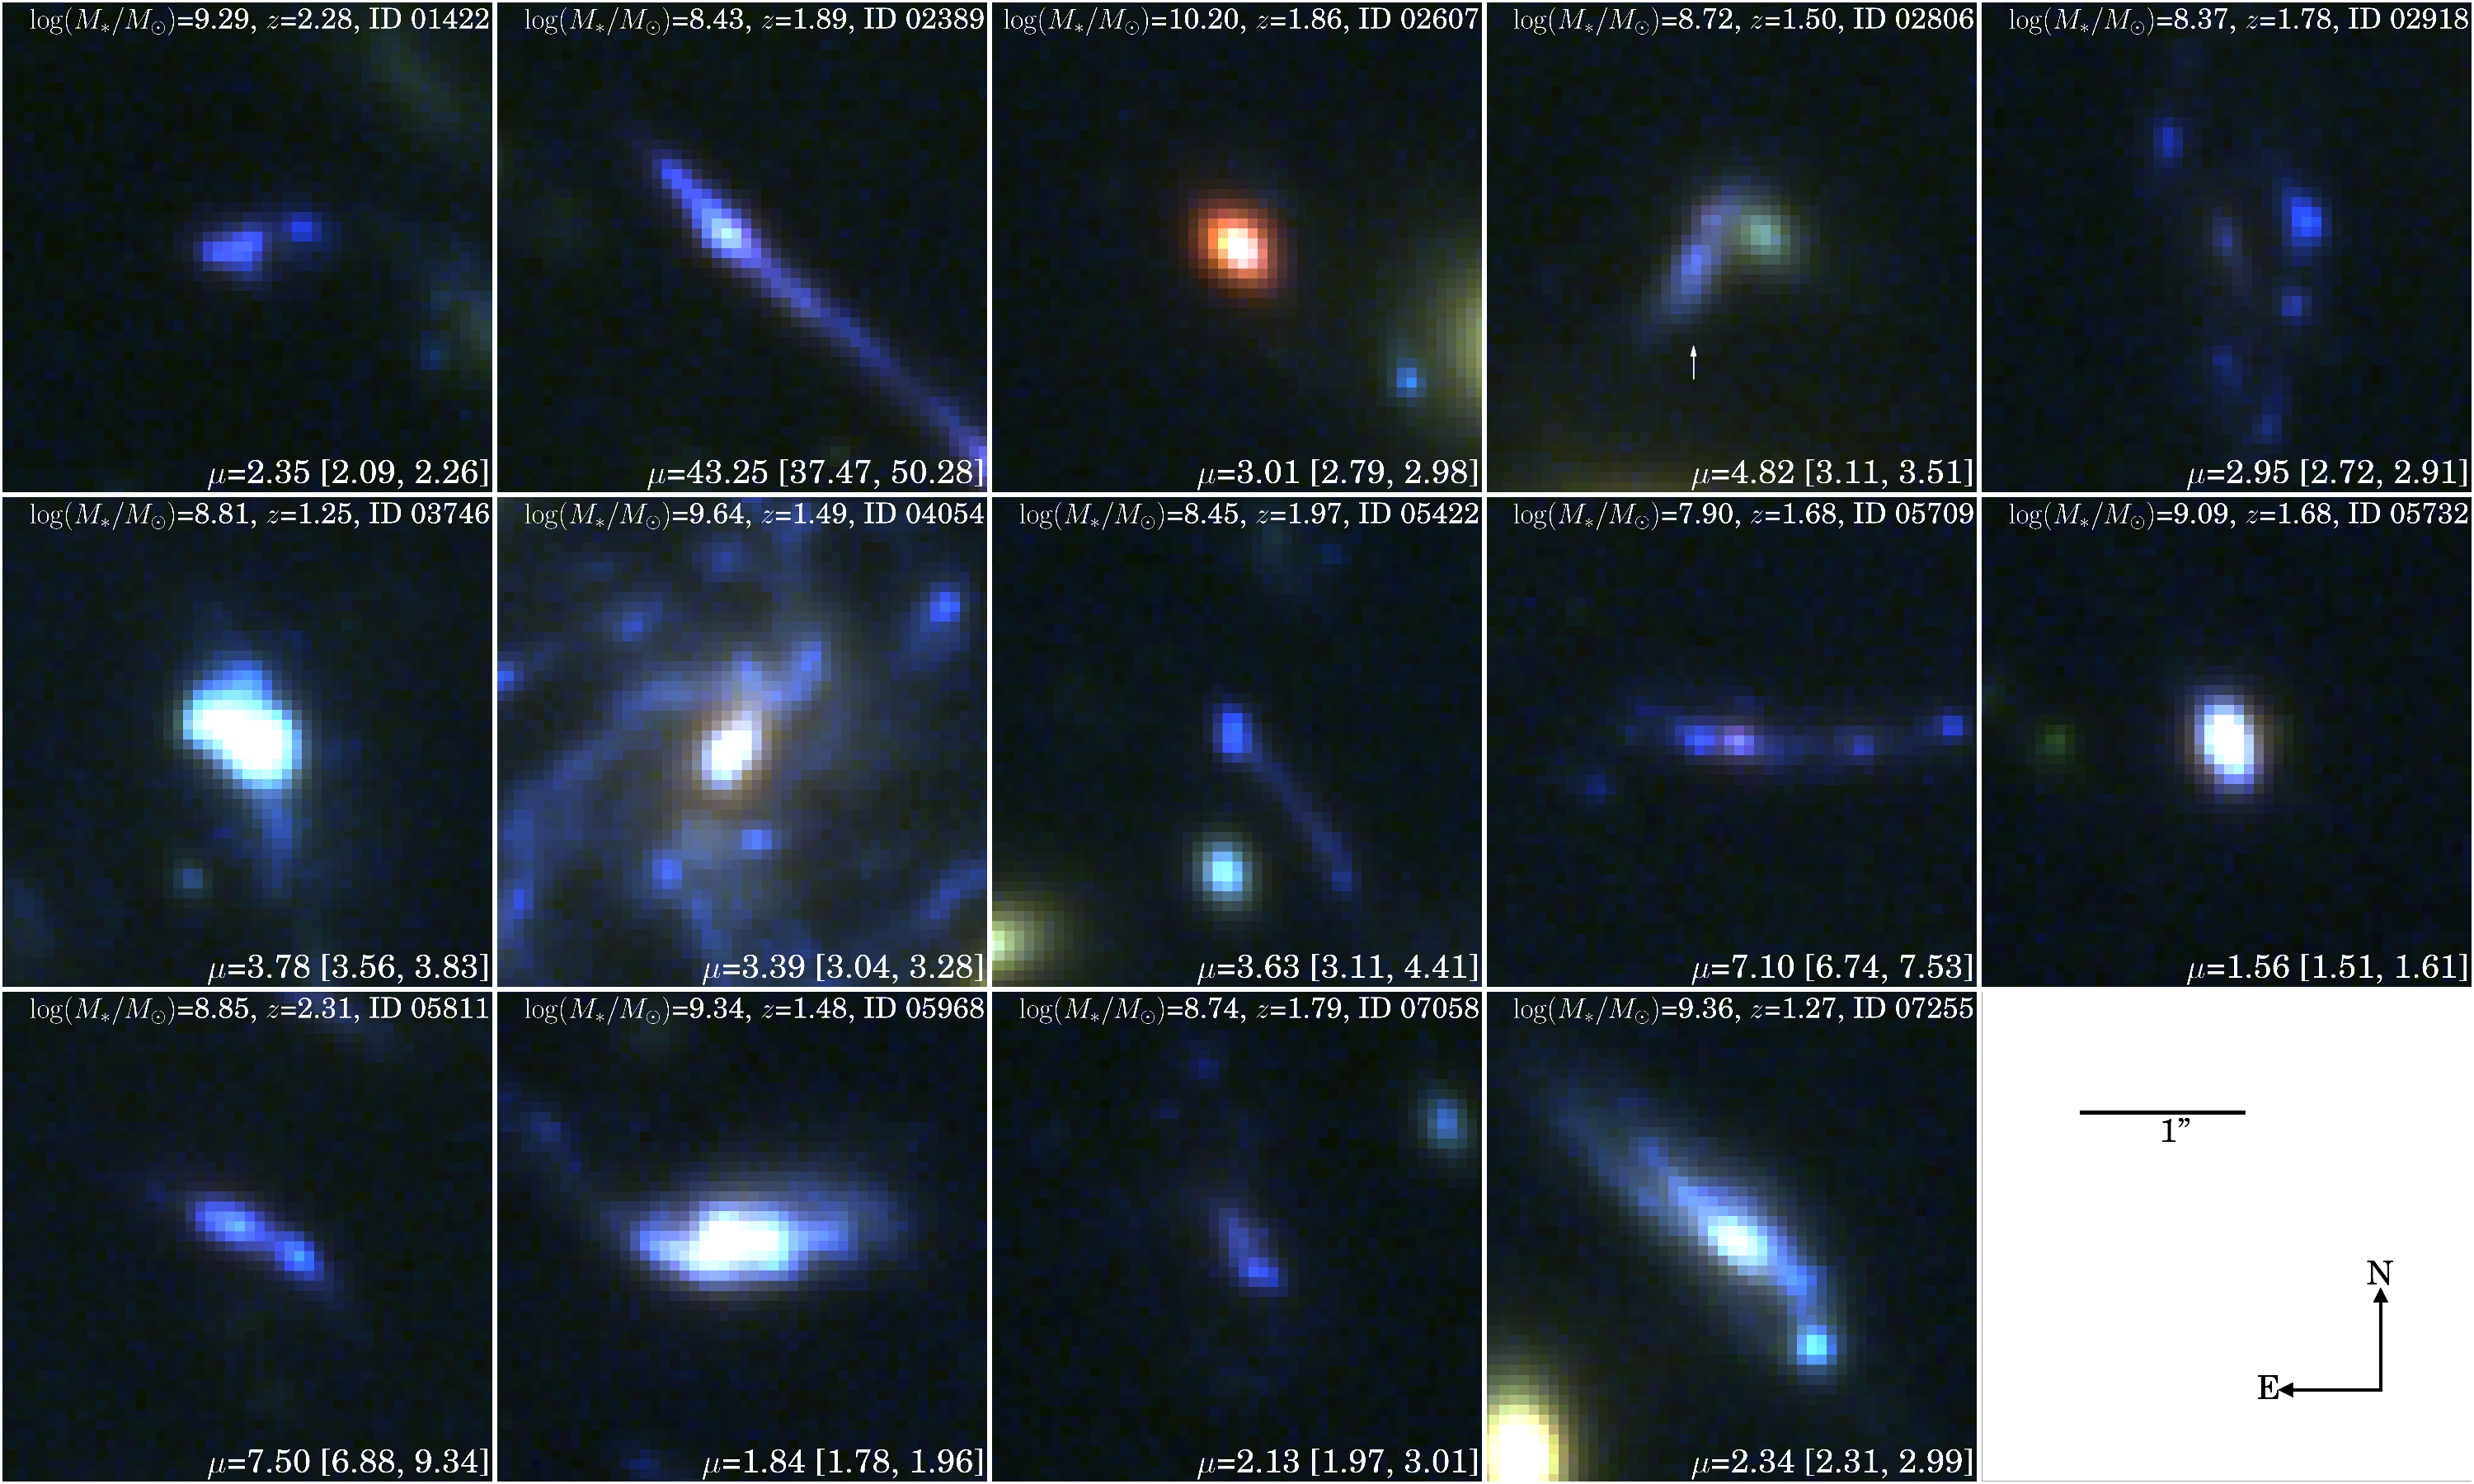
\includegraphics[width=\textwidth]{fig/frameRGBimg14src_hires.pdf}
    \caption[Zoom-in color composite stamps of our \mg sample.]{Zoom-in color composite stamps of our \mg sample, cut out from the full FoV
    image shown in Figure~\ref{fig:RGBfullFoV}. In each stamp, we also show the spectroscopic
    redshift, stellar mass and lensing magnification (best-fit value followed by 1-$\sigma$
    confidence interval) of the galaxy.
    In the panel of ID 02806, we use the white arrow to point to our galaxy of interest (ID
    02806). All stamps are on the same spatial scale. The 1\arcsec scale bar and north-east
    compass are shown in the lower right corner.}
    \label{fig:RGBstamps}
\end{figure}

For the purpose of this study, we compiled an exhaustive list of spatially extended sources with secure spectroscopic redshift
measurements in the range of $z\in[1.2, 2.3]$, showing strong ELs (primarily \OIII and \Hb) in the 2D grism spectra.
The reason this redshift range is selected is that we require high signal-to-noise ratio (SNR) detections of \OIII, \Hb and \OII 
ELs in the spectral region where grism sensitivity and throughput do not drop significantly, in order to deliver reliable 
metallicity estimates from well-calibrated EL diagnostics\footnote{The \Ha EL is only accessible in sources at $z\leq1.5$ in our 
sample. The \glass spectra of an exemplary galaxy whose \Ha is covered are displayed in Appendix~\ref{sect:ELflux}.}.
The selection results in a sample of 14 galaxies. The positions of these 14 galaxies relative to the cluster are denoted by the 
magenta circles in Figure~\ref{fig:RGBfullFoV}, while the postage stamp images of these galaxy are shown in 
Figure~\ref{fig:RGBstamps}.
The full sample is also listed in Table~\ref{tab:srcprop}.
In particular, one source in our sample, \ie, galaxy ID 04054, is one of the multiple images of SN Refsdal's host
galaxy (see Figure~\ref{fig:multiP_4054} for its appearances from
various perspectives). A steep metallicity gradient ($-0.16\pm0.02$
dex/kpc) has been previously measured on another multiple image of
this spiral galaxy \citep{Yuan:2011hj}. Our work is the first
\mgm on this particular image, which is least distorted/contaminated
by foreground cluster members. We also take advantage of a more
precise lens model of both the entire cluster and the SN Refsdal host,
from the extensive lens modeling effort summarized by \citet{2015arXiv151005750T}.

\begin{figure}
    \includegraphics[width=.33\textwidth]{fig_RGBstamps/rgbstamp_ID04054_4arcs.pdf}
    \includegraphics[width=.33\textwidth]{fig_mstarmaps/mstar_id04054_4arcs.pdf}
	\includegraphics[width=.33\textwidth]{fig_combELmaps/id04054_Ha.pdf}\\
	\includegraphics[width=.33\textwidth]{fig_combELmaps/id04054_OIII.pdf}
	\includegraphics[width=.33\textwidth]{fig_combELmaps/id04054_Hb.pdf}
	\includegraphics[width=.33\textwidth]{fig_combELmaps/id04054_OII.pdf}
    \caption[Multi-perspective view of the SN Refsdal host galaxy multiple image 1.3, \ie, ID 04504 in our
    sample.]
    {Multi-perspective view of the SN Refsdal host galaxy multiple image 1.3, \ie, ID
    04054 in our \mg sample.  \textit{Upper left}: zoom-in color composite stamp cut out from
    Figure~\ref{fig:RGBfullFoV}, where the estimated site of the un-observed past appearance
    of SN Refsdal is denoted by the red circle. \textit{Upper middle}: stellar mass surface
    density map for this galaxy, where the source plane de-projected galactocentric radius
    contours are overlaid, in 2 kpc intervals, starting from 1 kpc.  \textit{Upper right}:
    \Ha surface brightness map combined from the \hst grism exposures at all PAs from the
    \glass and Refsdal follow-up programs.
    The black contours again show the de-projected galactocentric radii in the same fashion
    presented in the stellar mass surface density map in the upper middle panel.
    \textit{Lower rows}: combined surface brightness maps of \OIII, \Hb, and \OII, presented
    in the same fashion as in the \Ha emission line map in the upper right panel.}
    \label{fig:multiP_4054}
\end{figure}


\section{Photometry and Lens Models from the \hff}\label{sect:phot}

The Hubble Frontier Fields
initiative\footnote{\url{http://www.stsci.edu/hst/campaigns/frontier-fields}} \citep[\hff;
P.I.  Lotz,][]{Lotz:2016ca} is an ongoing multi-cycle treasury program enabled by an \hst
director's discretionary time allocation. \hff targets the cores (prime fields) and infall regions (parallel fields)
of six massive galaxy clusters, reaching an ultra-faint intrinsic magnitude of 30-33, made possible by the synergy of diffraction
limited photometry and lensing magnification. The large wavelength coverage, uninterrupted from \B to \H passbands, is crucial for
photometric redshift determinations and stellar population synthesis.

Besides the deep image mosaics, the \hff collaboration also provides
the community with cluster lens models
\footnote{\url{http://archive.stsci.edu/prepds/frontier/lensmodels/}}.
Several groups of scientists were invited prior to the beginning of
the campaign to provide independent models depicting the total mass distribution
of the six \hff clusters, using a number of distinct techniques.
As data accumulate and more multiply imaged systems are identified, the lens models are continuously improved.
For our cluster of interest, \clyi, the most up-to-date publicly available model is the \glafic version 3 model,
constructed using a simply parametrized method proposed by \citet{2010PASJ...62.1017O}.
For an in-depth description of the various modeling techniques, their advantages and limitations, we
refer to \citet{2015arXiv151005750T,Meneghetti:2016wg}.

In this work, we need lens models to trace the observed metallicity
maps back to the source plane. Following our previous work \citep{2015AJ....149..107J},
we experiment with several publicly available models to find the ones that give the
reconstruction of our target sources the highest fidelity (judging by
how well the source plane morphologies of multiply imaged sources
match each other). Based upon the SN Refsdal test (see also \citet{2015arXiv151204654K}),
the \glafic version 3 model \citep{2015arXiv151006400K}, the \textsc{Grillo} model \citep{2016ApJ...822...78G}, and
the \SJ version 3 model were the most accurate ones, so we considered those three.
As an illustration, the \glafic version 3 critical curves at $z=1.8$, the
median redshift of our \mg sample, are overlaid in cyan in Figure~\ref{fig:RGBfullFoV}.

The most highly magnified source in our sample is galaxy ID 02389, one of
the folded arcs which straddle the critical curve. For that particular
source, we used as our default the \SJ version 3 model, updated from the earlier versions
presented in \citet{Johnson:2014cf,Sharon:2015hr}. The \SJ version 3 model leads
to a more precise reconstruction of the source plane morphology of
galaxy ID 02389.  We also tested that switching entirely from the
\glafic version 3 model to the \SJ version 3 model does not affect our
measurements significantly, as also pointed out by \citet{2015arXiv150901279L}.
The lensing magnification results from the considered lens models are given in
Table~\ref{tab:srcprop}.


\section{Analysis Procedures}\label{sect:analysis}

Here we describe the stellar population synthesis analysis of our sample in
Section~\ref{subsect:sed}, and source plane morphology reconstruction in
Section~\ref{subsect:morph}.
The entire steps necessary for extracting EL maps from 2D grism spectra combined from
different PAs are detailed in Section~\ref{subsect:combELmaps}.
Our new Bayesian method to jointly infer metallicity, nebular dust extinction, and SFR from a
simultaneous use of multiple strong ELs is presented in Section~\ref{subsect:bayes}.

\subsection{Spectral Energy Distribution Fitting}\label{subsect:sed}

The full-depth 7-filter \hff photometry was fitted with the template spectra from
\citet{Bruzual:2003ck} using the stellar population synthesis code \fast
\citep{Kriek:2009cs}, in order to derive global estimates of stellar mass (\Mstar) and the
dust extinction of stellar continuum ($\Av^{\rm S}$) for each source in our sample. We take a
grid of stellar population parameters that include: exponentially declining star formation
histories with $e$-folding times ranging from 10~Myr to 10~Gyr, stellar ages ranging from 5~Myr to
the age of the universe at the observed redshift, and $\Av^{\rm S}$=0-4 magnitudes for a
\citet{Calzetti:2000iy} dust extinction law. We assume the \citet{Chabrier:2003ki}
initial mass function (IMF) and fix the stellar metallicity to solar.
Table~\ref{tab:srcprop} lists the best-fit \Mstar values, corrected for lensing
magnification.
Although the adopted solar metallicity is higher than the typical gas-phase abundances we
infer for the sample, this has little effect on the derived stellar mass. Fixing the stellar
metallicity to $1/5$ solar (i.e. $Z=0.004$ or $\oh=8.0$, corresponding to the sample median)
reduces the best-fit \Mstar by only $\sim0.03$ dex.

\subsection{Source Plane Morphology}\label{subsect:morph}

Measurements of metallicity gradients require knowledge of the galaxy center, major axis orientation, and inclination or
axis ratio. We derive these quantities from spatially resolved maps of the stellar mass surface density following the
methodology described in \citet{2015AJ....149..107J}. Briefly, we smooth the \hff photometric
images to a common point spread function of 0\farcs2 FWHM and fit the spectral energy
distribution (SED) of each spaxel using the same procedure described in
Section~\ref{subsect:sed}. The resulting \Mstar maps in the image plane are shown in Figures~\ref{fig:multiP_4054} and
\ref{fig:multiP_rest}. We reconstruct the \Mstar maps in the source plane using the adopted
lens models and determine the centroid, axis ratio, inclination and major axis orientation from a 2D
elliptical Gaussian fit to the \Mstar distribution. This allows us to measure the
galactocentric radius at each point, assuming that contours of \Mstar surface density
correspond to constant de-projected radius \citep[following][]{2015AJ....149..107J}. 

Since the following analysis is mostly done with the robust image plane data, we reconstruct
the derived radius maps in the image plane.
The contours of constant source-plane galactocentric radius for each galaxy in our sample are shown in 
Figures~\ref{fig:multiP_4054} and \ref{fig:multiP_rest}. Note that these contours are distorted from ellipses ascribed to the 
shear of gravitational lensing.
For nearly half of our sample where we have seeing-limited IFU data described in Appendix~\ref{sect:kinem}, we verify that for 
galaxies with significant rotation support (\eg IDs 05709 and 05968), the morphological major axis agrees at 2-$\sigma$ with
the pseudo-slit that maximizes velocity shear according to our kinematic analysis.

\begin{figure}
    \includegraphics[width=.161\textwidth]{fig_RGBstamps/rgbstamp_ID01422.pdf}
    \includegraphics[width=.161\textwidth]{fig_mstarmaps/mstar_id01422.pdf}
    \includegraphics[width=.161\textwidth]{fig/baiban.png}
    \includegraphics[width=.161\textwidth]{fig_combELmaps/id01422_OIII.pdf}
    \includegraphics[width=.161\textwidth]{fig_combELmaps/id01422_Hb.pdf}
    \includegraphics[width=.161\textwidth]{fig_combELmaps/id01422_OII.pdf}\\
    \includegraphics[width=.161\textwidth]{fig_RGBstamps/rgbstamp_ID02389.pdf}
    \includegraphics[width=.161\textwidth]{fig_mstarmaps/mstar_id02389.pdf}
    \includegraphics[width=.161\textwidth]{fig/baiban.png}
    \includegraphics[width=.161\textwidth]{fig_combELmaps/id02389_OIII.pdf}
    \includegraphics[width=.161\textwidth]{fig_combELmaps/id02389_Hb.pdf}
    \includegraphics[width=.161\textwidth]{fig_combELmaps/id02389_OII.pdf}\\
    \includegraphics[width=.161\textwidth]{fig_RGBstamps/rgbstamp_ID02607.pdf}
    \includegraphics[width=.161\textwidth]{fig_mstarmaps/mstar_id02607.pdf}
    \includegraphics[width=.161\textwidth]{fig/baiban.png}
    \includegraphics[width=.161\textwidth]{fig_combELmaps/id02607_OIII.pdf}
    \includegraphics[width=.161\textwidth]{fig_combELmaps/id02607_Hb.pdf}
    \includegraphics[width=.161\textwidth]{fig_combELmaps/id02607_OII.pdf}\\
    \includegraphics[width=.161\textwidth]{fig_RGBstamps/rgbstamp_ID02806.pdf}
    \includegraphics[width=.161\textwidth]{fig_mstarmaps/mstar_id02806.pdf}
    \includegraphics[width=.161\textwidth]{fig_combELmaps/id02806_Ha.pdf}
    \includegraphics[width=.161\textwidth]{fig_combELmaps/id02806_OIII.pdf}
    \includegraphics[width=.161\textwidth]{fig_combELmaps/id02806_Hb.pdf}
    \includegraphics[width=.161\textwidth]{fig_combELmaps/id02806_OII.pdf}\\
    \includegraphics[width=.161\textwidth]{fig_RGBstamps/rgbstamp_ID02918.pdf}
    \includegraphics[width=.161\textwidth]{fig_mstarmaps/mstar_id02918.pdf}
    \includegraphics[width=.161\textwidth]{fig/baiban.png}
    \includegraphics[width=.161\textwidth]{fig_combELmaps/id02918_OIII.pdf}
    \includegraphics[width=.161\textwidth]{fig_combELmaps/id02918_Hb.pdf}
    \includegraphics[width=.161\textwidth]{fig_combELmaps/id02918_OII.pdf}\\
    \includegraphics[width=.161\textwidth]{fig_RGBstamps/rgbstamp_ID03746.pdf}
    \includegraphics[width=.161\textwidth]{fig_mstarmaps/mstar_id03746.pdf}
    \includegraphics[width=.161\textwidth]{fig_combELmaps/id03746_Ha.pdf}
    \includegraphics[width=.161\textwidth]{fig_combELmaps/id03746_OIII.pdf}
    \includegraphics[width=.161\textwidth]{fig_combELmaps/id03746_Hb.pdf}
    \includegraphics[width=.161\textwidth]{fig_combELmaps/id03746_OII.pdf}
    \caption[Multi-perspective view of our \mg sample.]{Multi-perspective view of our \mg sample except for the SN Refsdal host which is
    shown in Figure~\ref{fig:multiP_4054}.
    In each row, we show the zoom-in color composite stamp (the same as that in
    Figure~\ref{fig:RGBstamps}), the stellar mass surface density map, the combined surface
    brightness maps of \Ha (if available given object redshift), \OIII, \Hb, \OII for each
    object.
    The black contours overlaid represent the source plane de-projected galactocentric radii
    in 2 kpc interval, starting from 1 kpc. The spatial extent and orientation of the stamps
    for each object have been fixed.
    The typical surface brightness 1-$\sigma$ uncertainty in these combined EL maps is $2\times10^{-16}$ \SBunit.}
    \label{fig:multiP_rest}
\end{figure}
\begin{figure}
    \includegraphics[width=.161\textwidth]{fig_RGBstamps/rgbstamp_ID05422.pdf}
    \includegraphics[width=.161\textwidth]{fig_mstarmaps/mstar_id05422.pdf}
    \includegraphics[width=.161\textwidth]{fig/baiban.png}
    \includegraphics[width=.161\textwidth]{fig_combELmaps/id05422_OIII.pdf}
    \includegraphics[width=.161\textwidth]{fig_combELmaps/id05422_Hb.pdf}
    \includegraphics[width=.161\textwidth]{fig_combELmaps/id05422_OII.pdf}\\
    \includegraphics[width=.161\textwidth]{fig_RGBstamps/rgbstamp_ID05709.pdf}
    \includegraphics[width=.161\textwidth]{fig_mstarmaps/mstar_id05709.pdf}
    \includegraphics[width=.161\textwidth]{fig/baiban.png}
    \includegraphics[width=.161\textwidth]{fig_combELmaps/id05709_OIII.pdf}
    \includegraphics[width=.161\textwidth]{fig_combELmaps/id05709_Hb.pdf}
    \includegraphics[width=.161\textwidth]{fig_combELmaps/id05709_OII.pdf}\\
    \includegraphics[width=.161\textwidth]{fig_RGBstamps/rgbstamp_ID05732.pdf}
    \includegraphics[width=.161\textwidth]{fig_mstarmaps/mstar_id05732.pdf}
    \includegraphics[width=.161\textwidth]{fig/baiban.png}
    \includegraphics[width=.161\textwidth]{fig_combELmaps/id05732_OIII.pdf}
    \includegraphics[width=.161\textwidth]{fig_combELmaps/id05732_Hb.pdf}
    \includegraphics[width=.161\textwidth]{fig_combELmaps/id05732_OII.pdf}\\
    \includegraphics[width=.161\textwidth]{fig_RGBstamps/rgbstamp_ID05811.pdf}
    \includegraphics[width=.161\textwidth]{fig_mstarmaps/mstar_id05811.pdf}
    \includegraphics[width=.161\textwidth]{fig/baiban.png}
    \includegraphics[width=.161\textwidth]{fig_combELmaps/id05811_OIII.pdf}
    \includegraphics[width=.161\textwidth]{fig_combELmaps/id05811_Hb.pdf}
    \includegraphics[width=.161\textwidth]{fig_combELmaps/id05811_OII.pdf}\\
    \includegraphics[width=.161\textwidth]{fig_RGBstamps/rgbstamp_ID05968.pdf}
    \includegraphics[width=.161\textwidth]{fig_mstarmaps/mstar_id05968.pdf}
    \includegraphics[width=.161\textwidth]{fig_combELmaps/id05968_Ha.pdf}
    \includegraphics[width=.161\textwidth]{fig_combELmaps/id05968_OIII.pdf}
    \includegraphics[width=.161\textwidth]{fig_combELmaps/id05968_Hb.pdf}
    \includegraphics[width=.161\textwidth]{fig_combELmaps/id05968_OII.pdf}\\
    \includegraphics[width=.161\textwidth]{fig_RGBstamps/rgbstamp_ID07058.pdf}
    \includegraphics[width=.161\textwidth]{fig_mstarmaps/mstar_id07058.pdf}
    \includegraphics[width=.161\textwidth]{fig/baiban.png}
    \includegraphics[width=.161\textwidth]{fig_combELmaps/id07058_OIII.pdf}
    \includegraphics[width=.161\textwidth]{fig_combELmaps/id07058_Hb.pdf}
    \includegraphics[width=.161\textwidth]{fig_combELmaps/id07058_OII.pdf}\\
    \includegraphics[width=.161\textwidth]{fig_RGBstamps/rgbstamp_ID07255.pdf}
    \includegraphics[width=.161\textwidth]{fig_mstarmaps/mstar_id07255.pdf}
    \includegraphics[width=.161\textwidth]{fig_combELmaps/id07255_Ha.pdf}
    \includegraphics[width=.161\textwidth]{fig_combELmaps/id07255_OIII.pdf}
    \includegraphics[width=.161\textwidth]{fig_combELmaps/id07255_Hb.pdf}
    \includegraphics[width=.161\textwidth]{fig_combELmaps/id07255_OII.pdf}
    \contcaption{(cont.)}
\end{figure}

\subsection{Emission Line Maps from Grism Spectra}\label{subsect:combELmaps}

The broad grism wavelength coverage provides spatially resolved maps of multiple ELs,
such as \OII, \Hg, \Hb, \OIII, \Ha$+$\NII, and \SII.
The integrated fluxes of these ELs for our sample of galaxies are presented in Appendix~\ref{sect:ELflux}.
To obtain pure EL maps, we first use the \axe continuum models described in Section~\ref{sect:spec} to subtract contaminating
flux from neighboring sources. The continuum model for the target object is scaled to match
the locally observed levels, and then subtracted. We check that the flux residual in regions
near the ELs of interest follow a normal distribution with zero mean.

Due to the limited spectral resolution of \hst WFC3/IR grisms, \Hb and the \OIII$\lambda\lambda$4960,5008 doublets are
partially blended in the spatially extended sources. We adopt a direct de-blending technique
to separate these emission lines following the procedure used in \citet{2015AJ....149..107J}.
First, an isophotal contour is measured from the co-added \hst \H-band postage stamp,
typically at the level of $\sim$10 percent of the peak flux received from the source.
We then apply this contour to the 2D grism spectra at the observed wavelengths corresponding to
\OIII$\lambda\lambda$4960,5008 and \Hb, maximizing the flux given grism redshift uncertainty ($\sim$0.01).
We use the theoretical \OIII$\lambda\lambda$4960,5008 doublet flux ratio (\ie
\OIII$\lambda$5008/\OIII$\lambda$4960=2.98, calculated by \citet{Storey:2000jd}) to subtract
the flux contribution of \OIII$\lambda$4960 corresponding to the region where
\OIII$\lambda$5008 is unblended. We iterate this procedure to remove the \OIII$\lambda$4960
emission completely, resulting in pure maps of \Hb and \OIII$\lambda$5008.

Note that this direct de-blending will be compromised if the source is so extended that its
\OIII$\lambda$5008 and \Hb are blended. In practice, we fine-tune the isophotal contour level
to avoid this contamination. As a result, no cases in our sample have problem with our
direct de-blending method, and the resulting pure \OIII$\lambda$5008 and \Hb maps are
uncontaminated.

In the case of \Ha and \NII, the emission lines are separated by less than the grism spectral
resolution. Therefore we cannot use the direct technique to de-blend \Ha and \NII
emission, and instead treat the \NII/\Ha ratio as an unknown parameter in Section
\ref{subsect:bayes}.

After obtaining pure EL maps, we rotate the maps from each PA to the same orientation and then combine the data, in order 
to utilize the full depth of the grism exposures. We note that EL maps must first be extracted from grism spectra at each PA 
before being combined, in order to account for the different rotation and spectral resolution.
There are in total six different PA-grism combinations as given in Table~\ref{tab:obsdata}. At certain redshifts, ELs are
visible in the overlapping region between the two grisms at $\lambda\in[1.08,1.15]~\micron$
resulting in up to six individual maps of the same EL. We use the data taken at
PA=$119^{\circ}$ as a reference, as this minimizes errors arising from rotating the various
PAs into alignment. We first apply a small vertical offset to each EL map to account for the
slight tilt of the spectral trace (i.e. known offset between the dispersion direction and the
x-axis of extracted spectra; \citealt{Brammer:2012bu}). Next, we apply a small horizontal
shift to correct for uncertainties in the wavelength calibration and redshift. Finally we
rotate each EL map to align it with the reference orientation at PA=$119^{\circ}$.  The best
values of these three alignment parameters are found by maximizing the normalized
cross-correlation coefficient (NCCF) in order to achieve optimal alignment of multiple PAs:
\be\label{eq:ccf}
    \textrm{NCCF}=\frac{1}{n}\Sigma_{x,y}\frac{\(S_\refe(x,y)-\avg{S_\refe}\)\(S_\pa(x,y)-\avg{S_\pa}\)}{\sigma_{S_\refe}\sigma_{S_\pa}}.
\ee
Here $S$ is the \subr profile for a specific EL, $S_\refe$ corresponds to the reference
alignment stamp adopted as the PA=$119^{\circ}$ data, and $n$ is the number of spaxels in the
\subr profile. $\avg{S}$ and $\sigma_S$ represent the average and standard deviation of the
\subr, respectively.

Once the data from each PA are aligned, we vet the EL maps from each PA-grism combination and
reject those which show significant contamination-subtraction residuals or grism reduction defects.  We
combine the remaining maps of a given EL using an inverse variance weighted average
in order to properly account for the different exposure times and noise levels.
The final combined maps of each EL for each galaxy are shown in Figures~\ref{fig:multiP_4054} and
\ref{fig:multiP_rest}.

\subsection{Line-flux-based Bayesian Inference of Metallicity}\label{subsect:bayes}

%= = = = = = = = = = = = = = = = = = = = = = = = = = = = = = = = = = = = = = = =
% = = = = = = = = = = = = = = = = = = = = = = = = = = = = = = = = = = = = = = = = = =
% Include this table with \input{filename.tex}
% To rotate in emulateapj do: \begin{turnpage}\input{filename.tex}\end{turnpage}
% To display it on multiple pages do: \LongTables\input{filename.tex}
% - - - - - - - - - - - - - - - - - - - - - - - - - - - - - - - - - - - - - - - - - -
{\setlength\tabcolsep{2pt}
\begin{deluxetable}{llclccccccccc} \tablecolumns{13}
\tablewidth{0pt}
\tablecaption{Sampling parameters and their prior information.}
% - - - - - - - - - - - - - - - - - - - - - - - - - - - - - - - - - - - - - - - - - -
\tablehead{
    \colhead{Set} &
    \colhead{Parameter} &
    \colhead{Symbol (Unit)} &
    \colhead{Prior}
}
%---------------------------------------------------------------
\startdata
Vanilla & \gpm & \oh & flat: $[7.0,9.3]$ \\
        & nebular dust extinction & $\Av^{\rm N}$ & flat: $[0,4]$ \\
        & de-reddened \Hb flux & $f_{\Hb}$ ($10^{-17}$\Funit) & Jeffrey's: $[0,100]$ \\
\hline\smallskip
Extended & \NII to \Ha flux ratio & \NII/\Ha & Jeffrey's: [0, 0.5] \\
\hline
Derived & \sfr &  SFR (\Msun/yr) &  ---
\enddata
% - - - - - - - - - - - - - - - - - - - - - - - - - - - - - - - - - - - - - - - - - -
\tablecomments{Most constraints presented in this work are obtained under the ``Vanilla'' parameter set with the extended
parameter fixed as \NII/\Ha=0.05.}
\label{tab:param}
\end{deluxetable}

%= = = = = = = = = = = = = = = = = = = = = = = = = = = = = = = = = = = = = = = =

Generally speaking, two methods exist in deriving gas-phase oxygen abundance in star-forming galaxies at high redshifts.
``Direct'' determinations based on electron temperature measurements, which require high SNR
detections of auroral lines (\eg \OIII$\lambda$4364), are still extremely challenging beyond the local universe \citep[see][for a
rare example]{Sanders:2016uo}.
We therefore rely on the calibrations of strong collisionally excited EL flux ratios to estimate metallicities.

One of the most popular strong EL diagnostics is the flux ratio of \NII/\Ha calibrated by \citet{2004MNRAS.348L..59P}.  However, a
large offset (0.2-0.4 dex) between the loci of high-$z$ and present-day star-forming galaxies in the Baldwin-Phillips-Terlevich
\citep[BPT,][]{Baldwin:1981ev} diagram has recently been discovered, indicating that extending the locally calibrated \NII/\Ha to
high-$z$ can be problematic \citep{2015ApJ...801...88S,Sanders:2015gk}.  The interpretation of this offset is still the topic of
much debate. It has been interpreted as the existence of a fundamental relation between nitrogen-oxygen abundance ratio and \Mstar
\citep{Masters:2016vr}, a systematic dependence of strong EL properties with respect to Balmer line luminosity
\citep{Cowie:2016fv}, a combination of harder ionizing radiation and higher ionization states of the ISM gas at high redshifts.
\citep{2014ApJ...795..165S,Steidel:2016wu}, or an enhancement of nitrogen abundance in hot \HII regions \citep{Pilyugin:2010bx}.  
Fortunately, the alpha-element BPT diagrams show no offset with $z$ \citep{2015ApJ...801...88S,Sanders:2015gk}, and therefore the 
diagnostics based upon those ELs are more reliable.

In this work we adopt the calibrations of \citet[M08]{2008A&A...488..463M}, including the flux ratios of \OIII/\Hb, \OII/\Hb,
\NII/\Ha.
Given the potential systematics related to nitrogen ELs, we do not use the \NII/\Ha calibration of M08.
M08 fit the relation between these EL ratios and gas-phase oxygen abundance based upon ``direct'' measurements (from
\OIII$\lambda$4364) for \oh$<8.3$, and photoionization model results for higher metallicities. This provides a continuous
framework valid over the wide range \oh$\in(7.1,9.2)$.  We note that although there are alternative calibrations of metallicity
available in the literature and the applicability of these recipes is currently a hotly debated topic \citep[see,
\eg,][]{Blanc:2015hl,Dopita:2013bj}.  Here we are primarily interested in relative metallicity measurements.  Even though the
absolute measurements of metallicity may change if we used a different calibration, the gradients and morphological features in
the maps should be more robust to changes in the calibration. We will restrict our comparisons with other samples to only include
studies assuming the M08 calibrations.

Unlike previous work in which calibrated relations are applied to
various EL flux ratios \citep[see, \eg,][]{PerezMontero:2014jh,Bianco:2015hn}, we design a Bayesian statistical approach which
uses directly the individual EL fluxes as input, such that the information from one EL is only used once.
Our approach presents several advantages over those based on line flux ratios.
First, it properly accounts for flux uncertainties for lines that are weak
or undetected. Second, multiple lines can be taken into consideration
without the risk of double counting any information.

Our approach simultaneously infers gas-phase metallicity (\oh),
nebular dust extinction ($\Av^{\rm N}$), and expected de-reddened \Hb flux in units of $10^{-17}$\Funit.
Details of the prior assumptions applied to these parameters are explained in Table~\ref{tab:param}.
For values of these three parameters we can compute the expected line
fluxes, and compare with measured values to compute the likelihood and
then the posterior probability.
The \chisq statistic in our inference procedure is calculated as
\begin{equation}\label{eqn:chi2}
    \chisq = \sum_i \frac{\(f_{\el{i}} - R_i \cdot f_{\Hb}\)^2}
        {\(\sigma_{\el{i}}\)^2 + \(f_{\Hb}\)^2\cdot\(\sigma_{R_i}\)^2}.
\end{equation}
Here \el{i} denotes the set of emission lines \OII, \Hg, \Hb, \OIII, \Ha, and \SII. $f_{\el{i}}$ and $\sigma_{\el{i}}$ represent 
the observed de-reddened \el{i} flux and its uncertainty given a value of $\Av^{\rm N}$. We adopt the \citet{1989ApJ...345..245C} 
galactic extinction curve with \Rv=3.1.
$R_i$ is the dust-corrected flux ratio between \el{i} and \Hb, with $\sigma_{R_i}$ being the associated intrinsic scatter.
Note that the content of $R_i$ varies depending on the corresponding \el{i} in the following ways.

\indent\textbullet~ For $\el{i} \in \{\Ha,~\Hg\}$, $R_i$ corresponds to the Balmer decrement. We use the intrinsic Balmer ratios 
of $\Ha/\Hb=2.86$ and $\Hg/\Hb=0.47$, appropriate for case B recombination and fiducial \HII region conditions \citep[see, 
\eg,][]{Hummer:1987ed}. We set $\sigma_{R_i}=0$, assuming the intrinsic Balmer ratios are fixed with no scatter.
These ratios are proxies of the nebular dust extinction $\Av^{\rm N}$.

\indent\textbullet~ For $\el{i} \in \{\OII,~\OIII\}$, $R_i$ and $\sigma_{R_i}$ are taken from the M08 calibrations.
These ratios are diagnostics of the oxygen abundance \oh.

\indent\textbullet~ For $\el{i} = \SII$, we compute the values of $R_i$ and $\sigma_{R_i}$ using the Balmer ratio of $\Ha/\Hb$ and 
our new calibration of the ratio $\SII/\Ha$, derived following \citet{2015ApJ...813..126J}. \citet{2015ApJ...813..126J} used the 
same data as the low-metallicity calibrations of M08.
Although M08 do not provide any calibrations for \SII, we expect our calibration to be self-consistent and reliable for
$\oh\lesssim8.4$. \SII/\Ha is primarily useful as a diagnostic to differentiate between the
upper and lower branches of the \OIII/\Hb calibration. This is valuable because \NII is not
directly measured and \OII is typically low signal-to-noise in the lower redshift galaxies
for which \SII is available, due to decreasing grism throughput at $\lambda<0.9$ \micron.

\indent\textbullet~ For $\el{i} =$ \Hb, $R_i = 1$ with $\sigma_{R_i}=0$. This is just comparing the observed and expected \Hb 
flux, corrected for dust extinction.

\noindent
These EL flux ratios can be computed given a value of \oh, using a universal polynomial functional form, \ie, $\log{R} = 
\sum_{i=0}^{5}c_i\cdot x^i$, where $x=\oh-8.69$.
We summarize the coefficients ($c_i$) for each ratio diagnostic used in our statistical inference in Table~\ref{tab:ELratioCoef}.

In addition, the \NII/\Ha ratio is included as an additional parameter for galaxies at
$z\lesssim1.5$ where these lines are observed. However we do not attempt to determine \NII/\Ha using
the M08 calibrations, as locally-calibrated diagnostics tend to underestimate the \NII/\Ha
ratio in high-$z$ galaxies whereas oxygen and other $\alpha$-element line ratios remain
constant with redshift \citep{2014ApJ...795..165S,2015ApJ...801...88S,2015ApJ...813..126J}.
Instead we either leave this parameter free (``extended'' priors), or fixed to $\NII/\Ha=0.05$
(``vanilla'' priors).  The vanilla value is typical of galaxies with
similar $z$ and oxygen EL ratios as our sample.  Fixing the value of $\NII/\Ha$ provides
faster convergence and does not significantly affect the inferred metallicity.  We therefore
report constraints for the ``vanilla'' parameter set. For galaxy ID 04054, the
SN Refsdal host galaxy, we fix its \NII/\Ha to be 0.11, as measured by \citet{Yuan:2011hj}.

%The primary goal of the Bayesian inference is to determine metallicities. The posterior probability density distribution for
%metallicity is obtained after marginalizing over nuisance parameters, \ie,
%\begin{equation}
%    \cP(\oh) = \iint \exp(-\chisq/2) \cdot \cP_\textrm{prior}(f^\theo_{\Hb}) \d f^\theo_{\Hb} \cdot
%    \cP_\textrm{prior}(\Av^{\rm N}) \d \Av^{\rm N}.
%\end{equation}
We use the Markov Chain Monte Carlo sampler \emc \citep{ForemanMackey:2013io} to
explore the parameter space, setting the number of walkers to 100 with 5,000 iterations for each walker,
and a burnin of 2,000. The autocorrelation times are computed for
each parameter and are used to make sure chains have converged.
An example constraint result for the SN Refsdal host galaxy's global EL fluxes is shown in Figure~\ref{fig:corner}.
While this work is primarily concerned with gas-phase metallicities, our method simultaneously provides constraints on $\Av^{\rm N}$ and
SFR which can be compared to the results of SED fitting.
We then calculate the lensing-corrected de-reddened \Ha luminosity from $f_{\Hb}$ (assuming the fiducial Balmer ratio) and the 
magnification estimate of the source.
Then the instantaneous SFR can be derived, via the commonly-used calibration of \citet{Kennicutt:1998ki,Moustakas:2010ke}, \ie,
\be
    {\rm SFR} = 4.6\times10^{-42}~ \frac{L(\Ha)}{\rm erg/s} \quad [\Msun/\textrm{yr}],
\ee
valid for a \citet{Chabrier:2003ki} IMF. This SFR estimate does not rely on any assumptions about \sfh, and thus is a more direct 
measure of ongoing star formation than values given by SED fitting.

\begin{figure}
    \centering
    \includegraphics[width=\textwidth]{fig/corner_id04054.png}
    \caption[Marginalized 1D and 2D constraints from our Bayesian parameter inference.]{The marginalized 1D and 2D constraints on (\oh, $\Av^{\rm N}$, and
    $f_{\Hb}$), which are drawn from the integrated line fluxes of the Refsdal host
    galaxy (ID 04054), after all grism exposures are combined. The values on top of each
    column are the medians with 1-$\sigma$ uncertainties for each parameter. The plot in the
    upper right corner illustrates a good convergence of the sampling.}
    \label{fig:corner}
\end{figure}

%= = = = = = = = = = = = = = = = = = = = = = = = = = = = = = = = = = = = = = = =
% = = = = = = = = = = = = = = = = = = = = = = = = = = = = = = = = = = = = = = = = = =
% Include this table with \input{filename.tex}
% To rotate in emulateapj do: \begin{turnpage}\input{filename.tex}\end{turnpage}
% To display it on multiple pages do: \LongTables\input{filename.tex}
% - - - - - - - - - - - - - - - - - - - - - - - - - - - - - - - - - - - - - - - - - -
\begin{deluxetable}{ccccccccccccc} \tablecolumns{13}
\tablewidth{0pt}
\tablecaption{Coefficients for the EL flux ratio diagnostics used in our Bayesian inference.}
% - - - - - - - - - - - - - - - - - - - - - - - - - - - - - - - - - - - - - - - - - -
\tablehead{
    \colhead{$R$} & 
    \colhead{$c_0$} &
    \colhead{$c_1$} &
    \colhead{$c_2$} &
    \colhead{$c_3$} &
    \colhead{$c_4$} &
    \colhead{$c_5$}
}
%---------------------------------------------------------------
\startdata
\Ha/\Hb     &  0.4564 & \nodata & \nodata & \nodata & \nodata & \nodata \\
\Hg/\Hb     & -0.3279 & \nodata & \nodata & \nodata & \nodata & \nodata \\
\OIII/\Hb   &  0.1549 & -1.5031 & -0.9790 & -0.0297 & \nodata & \nodata \\
\OII/\Hb    &  0.5603 &  0.0450 & -1.8017 & -1.8434 & -0.6549 & \nodata \\
%\NeIII/\OII & -1.2608 & -1.0861 & -0.1470 & \nodata & \nodata & \nodata \\
\SII/\Ha    & -0.5457 &  0.4573 & -0.8227 & -0.0284 &  0.5940 &  0.3426
\enddata
% - - - - - - - - - - - - - - - - - - - - - - - - - - - - - - - - - - - - - - - - - -
\tablecomments{The value of EL flux ratio is calculated by the polynomial functional form,
\ie, $\log{R} = \sum_{i=0}^{5}c_i\cdot x^i$, where $x=\oh-8.69$. The ratio of \SII/\Ha is
calibrated by the work of \citet{2015ApJ...813..126J}, and the Balmer line ratios correspond
to the Balmer decrement, whereas the ratios between oxygen lines and \Hb are from M08.}
\label{tab:ELratioCoef}
\end{deluxetable}

%= = = = = = = = = = = = = = = = = = = = = = = = = = = = = = = = = = = = = = = =

We apply this inference procedure to both galaxy-integrated line
fluxes (to be discussed in Section~\ref{sect:global}) as well as
individual spaxels in the EL maps (which will lead to \mgms described
in Section~\ref{sect:sra}).

\section{Global Demographic Properties}\label{sect:global}

Based upon the Bayesian analysis, we obtain the global measurements of \gpm, nebular dust extinction, and SFR, for all sources in
our sample, as shown in Table~\ref{tab:srcprop}. First, we check for the presence of any active galactic nucleus (AGN)
contamination in our sample. Because not all galaxies in our sample reside in the redshift range where all BPT lines are
available, we resort to the mass-excitation diagram showing the \OIII/\Hb flux ratio as a function of \Mstar, first proposed by
\citet{Juneau:2011fz} to differentiate \sf galaxies and AGNs in local Sloan Digital Sky Survey (SDSS) observations.
\citet{Juneau:2014ca} further revised the demarcation scheme by applying line luminosity evolution and selection effects to a more
complete SDSS galaxy sample, and tested that this scheme agrees well with the bivariate distributions found in a number of
high-$z$ galaxy samples.
According to the \citet{Juneau:2014ca} classification scheme, all but one galaxy (ID 02607) have a negligible probability of being
AGN (see Figure~\ref{fig:MEx}).
Recently, \citet{Coil:2015dp} found that a +0.75 dex \Mstar shift in the \citet{Juneau:2014ca} scheme is required to avoid serious
AGN contamination in the \mosdef galaxy sample at $z\sim2.3$.
We verified that galaxy 02607 can still be safely classified as an AGN candidate, even considering the \citet{Coil:2015dp} shifted
classification scheme.
Because the M08 calibrations originate from \HII region observations and theoretical models, not designed for AGNs, our method
will not predict a reliable metallicity constraint for the AGN candidate ID 02607. We thereby exclude this source in the rest of
our population analysis. For the rest of our sample, comprising 13 star-forming galaxies, the constraint on \gpm is robust.

\begin{figure}
    \centering
    \includegraphics[width=\textwidth]{fig/MEx.pdf}
    \caption[Mass excitation diagnostic diagram.]{Mass excitation diagnostic diagram for our \mg sample. The curves are the
    demarcation lines updated by \citet{Juneau:2014ca}. The regions below the green curve
    have a low probability ($<10\%$) of being classified as AGNs, whereas galaxies located above the red curve are secure AGN
    candidates. In our sample, the only AGN candidate,  \ie, ID 02607, is marked by a square.}
    \label{fig:MEx}
\end{figure}

In Figure~\ref{fig:SFMS}, we plot the measured SFR as a function of \Mstar for our sample. In comparison, the loci of
mass-selected galaxies observed by the \kd survey and the ``\sfms'' \citep[SFMS,][]{Whitaker:2014ko,Speagle:2014dd} at similar
redshifts are also shown. We can see that selecting lensed galaxies based upon EL strength can probe deep into the low-mass regime
at high redshifts that is currently inaccessible to mass complete surveys. As expected, our emission line selected targets probe 
the
upper envelope of the SFMS, so that a detail comparison is non-trivial and should take into account the selection functions of
each sample. The advantage of the emission line selection technique is that it is the most cost-effective way to obtain gas
metallicities for stellar masses down to 10$^7$ \Mstar at $z\sim2$. Using the same technique, we discovered an analog of local
group dwarf spheroidals \citep[\eg, Fornax,][]{Coleman:2008ca} at $z=1.85$ experiencing active star formation (with 1 dex offset
from the SFMS), in our previous work \citep{2015AJ....149..107J}.

\begin{figure}
    \centering
    \includegraphics[width=\textwidth]{fig/SFMS.pdf}
    \caption[Star formation rate as a function of stellar mass for emission-line galaxies.]
    {Star formation rate as a function of stellar mass for emission-line galaxies at
    $z\in[1.2,2.3]$. Our \mg sample is marked by blue points; the
    literature sample is color-coded by reference according to the legend. The star-forming
    main sequence compiled by
    \citet{Speagle:2014dd} and \citet{Whitaker:2014ko} are represented by brown and orange
    lines respectively, where the dotted part is extrapolated at masses below the mass
    completeness limit.  The shaded regions denote the typical scatter of star-forming main
    sequence, \ie 0.2-0.3
    dex. We also show the source density contours for the \kd survey at the same redshift
    range, where 68\%, 95\%, and 99\% of all \kd galaxies at $z\in[1.2,2.3]$ can be found
    within the black solid, dashed, and dotted contours respectively.
    It is found that our sample is highly complementary to the \kd sample in terms of stellar
    mass.}
    \label{fig:SFMS}
\end{figure}


We also collect all published \gpm measurements in emission-line galaxies in the redshift range of our sample
$1.2\lesssim z\lesssim2.3$, obtained exclusively from the strong EL calibrations
prescribed by M08. The reason we only select measurements based upon
the M08 calibrations is that adopting different strong EL calibrations
can give rise to different absolute metallicity scales offset by up to
$\sim$0.7 dex at the high-mass end, according to the comparative study conducted by
\citet{Kewley:2008be}.  In order to minimize the systematic uncertainty associated with EL
calibrations, we thus focus on this homogeneous M08 sample alone.

As shown in Figure~\ref{fig:MZR}, the M08-based sample includes five galaxies from
\citet{2011MNRAS.413..643R}, seven from
\citet{Wuyts:2012gb}, six from \citet{Belli:2013cn}, four
stack measurements by \citet{Henry:2013gx}, three interacting galaxies
at $z=1.85$ analyzed by \citet{2015AJ....149..107J}, and 13
star-forming galaxies presented in this work.  In total, this sample
consists of 38 independent measurements at $1.2\lesssim z\lesssim2.3$, with median
redshift $z_{\rm median}=1.84$. The mutual agreement
between our sample and that from the literature provides an
independent confirmation that our new Bayesian method leads to
constraints on \gpm consistent with previous studies also adopting
the same calibrations.  With the combined sample we
are able to derive the MZR at this redshift, spanning three orders of magnitude in stellar
mass.

We fit the following functional form to this sample of 38 galaxies in order to derive the
MZR, \ie,
\begin{equation}
    \oh = \alpha\log\(\Mstar/\Msun\) + \beta + N(\sigma),
\end{equation}
where $\alpha$, $\beta$, and $\sigma$ represent the slope, the intercept and the intrinsic
scatter, respectively.
The Python package \linmix\footnote{available at \url{https://github.com/jmeyers314/linmix}}
was employed to perform a Bayesian linear regression following the method proposed by \citet{Kelly:2007bv}. The median values and
1-$\sigma$ uncertainties for these three parameters drawn from the marginalized posteriors are
\begin{equation}
    \alpha=0.40^{+0.07}_{-0.07},~~\beta=4.71^{+0.62}_{-0.64},~~\sigma=0.03^{+0.02}_{-0.01}.
\end{equation}
The resulting MZR together with its 1-$\sigma$ confidence region is shown in
Figure~\ref{fig:MZR}.

\begin{figure}
    \centering
    \includegraphics[width=\textwidth]{fig/MZR.pdf}
    \caption[The mass-metallicity relation at $z\sim1.8$.]{The relation between stellar mass and gas-phase oxygen abundance, from
    observations and simulations at $z\sim1.8$. The color-coding for all the points is the
    same as in Figure~\ref{fig:SFMS}. For the sake of consistency, all metallicity
    measurements are derived assuming the \citet{2008A&A...488..463M} strong EL calibrations.
    The black curves represent the 2nd order polynomials
    fitted by \citet{2008A&A...488..463M} to data sets at different redshifts, where dashed
    parts correspond to extensions beyond mass completeness limits of those data sets.  The
    thick brown line denotes our best-fit linear relation based upon all data
    points except the AGN candidate (\ie ID 02607) marked by a square.
    The shaded band marks the 1-$\sigma$ confidence region.  For the \citet{Henry:2013gx}
    stack data points, we also show the measurements without dust correction as open circles,
    which are not included in the fit.
    The thin orange line is the prediction from the cosmological zoom-in simulations
    conducted by \citet{Ma:2016gw} at the same redshift range.
    The purple dotted and dash-dot lines illustrate the slopes given by the energy and momemtum driven models, respectively.}
    \label{fig:MZR}
\end{figure}

Recently, \citet{Guo:2016wk} presented a comprehensive study of the MZR and its scatter at
$z$=0.5-0.7 from data acquired by large spectroscopic surveys in the \candels fields
\citep{Grogin:2011hx,Koekemoer:2011br}. \citet{Guo:2016wk} also summarized a variety of
theoretical predictions of the MZR slope (\ie $\alpha$) given by diverse approaches.
The slopes predicted by the energy-driven wind ($\alpha\sim0.33$) and the momentum-driven wind ($\alpha\sim0.17$)
equilibrium models proposed by \citet{2008MNRAS.385.2181F,2012MNRAS.421...98D} are shown schematically in Figure~\ref{fig:MZR}.
We see that our inferred slope is only marginally compatible with the prediction given by the
energy-driven wind model at 1-$\sigma$ confidence level, whereas strongly disfavors the
momentum-driven wind model. Considering the majority of the galaxies in our sample have
relatively lower masses, our result confirms the finding by \citet{Henry:2013gx} that
momentum-driven winds cannot be the primary workhorse that shapes the MZR in the low-mass
regime (below 10$^{9.5}$ \Msun) at $z\gtrsim1$.

Our constrained value of $\alpha$ is consistent at 1-$\sigma$ confidence level with that given by \citet{Ma:2016gw}, from the FIRE 
(Feedback in Realistic Environment) cosmological zoom-in simulations \citep{GalaxiesonFIREFe:2014dn}. Evaluated at $z=z_{\rm 
median}$, their MZR reads $\oh = 0.35 \log\(\Mstar/\Msun\) + 4.87$.
The FIRE simulations reaches a spatial resolution as high as 1-10 pc, 1-2 orders of magnitude better than that in conventional
large-volume cosmological hydrodynamic simulations \citep[\eg][]{2013MNRAS.434.2645D}. The high spatial resolution
enables a more realistic and self-consistent treatment of multiphase ISM, star formation,
galactic winds and stellar feedback, than those in semi-analytic models \citep[see][for a
recent review]{2015ARA&A..53...51S}.  As a result, these zoom-in simulations are capable of
reproducing many observed relations, \eg, the galaxy stellar mass functions, the evolution of
cosmic SFR density and specific SFR (sSFR).
The consistency between the slopes of our MZR and that by \citet{Ma:2016gw} indicates that small-scale physical processes are 
important in producing the cumulative effects of galactic feedback.
However, we note that there is a 0.16 dex offset in the values of the MZR intercept ($\beta$). One possible cause is that the 
absolute metallicity scale in the M08 calibrations is offset. As shown by \citet{Kewley:2008be}, the intercepts given by different 
metallicity calibrations can vary up to 0.7 dex. Other potential causes lie in the assumptions adopted by the \citet{Ma:2016gw} 
simulations, \eg, the stellar yield is too small, the gas fractions in their simulated galaxies are too high, \etc.
Nevertheless, a discrepancy of 0.1-0.2 dex is not unusual given the uncertainties in stellar yield and metallicity calibrations.

Aiming at testing the validity of the FMR using the M08-based sample at $z\sim1.84$ compiled
in this work, we calculate the predicted values for metallicity from the measurements of
\Mstar and SFR, according to Eq.~(2) in \citet{Mannucci:2011be}, who extended the FMR to
masses down to $10^{8.3}\Msun$.
Figure~\ref{fig:FMR} shows the difference between the FMR-predicted
values and the actual measurements of metallicity.  We find that the entire
M08-based sample is consistent with the FMR given the measurement
uncertainties and intrinsic scatter. The median offset for the entire
sample is 0.07 dex, with median uncertainty 0.14 dex.
The median offset and uncertainty for our galaxy sample analyzed in this work are $-0.07$ dex and 0.12 dex, respectively. Among
other individual datasets, the only one that shows a
marginally significant deviation from the FMR is that by
\citet{Wuyts:2012gb}, which has median offset 0.22 dex and median
uncertainty 0.11 dex. We speculate that it is due to the fact that the
\citet{Wuyts:2012gb} dataset is the only one in our compiled M08-based
sample which relies solely upon the \NII/\Ha flux ratio, which can be
a biased tracer of metallicity at high redshifts \citep{2015ApJ...801...88S,Sanders:2015gk}.
This result reiterates the necessity of combining multiple EL flux ratio diagnostics
simultaneously in order to suppress the systematics associated with local calibrations in the
accurate measurement of high-$z$ metallicity.

\begin{figure}
    \centering
    \includegraphics[width=\textwidth]{fig/FMRoffset.pdf}
    \caption[Offset from the fundamental metallicity relation.]{The offset from the fundamental metallicity relation first proposed by
    \citet{2010MNRAS.408.2115M} for the $z\sim1.8$ metallicity measurements derived assuming
    the \citet{2008A&A...488..463M} calibrations.  The color-coding for the points is the
    same as in Figure~\ref{fig:SFMS}.  The shaded region shows the intrinsic scatter of the
    FMR extended to low-mass regime given by
    \citet{Mannucci:2011be}.}
    \label{fig:FMR}
\end{figure}

\section{Spatially Resolved Analysis}\label{sect:sra}

In this section, we present and discuss in depth the new and unique results obtained from the spatially resolved analysis of our
sample, beyond the reach of the conventional integrated measurements in Section~\ref{sect:global}.
The high spatial resolution maps of \gpm from \hst grism spectroscopy are described in Sect~\ref{subsect:oh12grad}.
We make notes on individual galaxies in Section~\ref{subsect:indvd}.
The maps of EL kinematics on part of our sample are presented in Appendix~\ref{sect:kinem}.

\subsection{Gas-phase Metallicity Maps at Sub-kpc Resolution}\label{subsect:oh12grad}

%= = = = = = = = = = = = = = = = = = = = = = = = = = = = = = = = = = = = = = = =
% = = = = = = = = = = = = = = = = = = = = = = = = = = = = = = = = = = = = = = = = = =
% Include this table with \input{filename.tex}
% To rotate in emulateapj do: \begin{turnpage}\input{filename.tex}\end{turnpage}
% To display it on multiple pages do: \LongTables\input{filename.tex}
% - - - - - - - - - - - - - - - - - - - - - - - - - - - - - - - - - - - - - - - - - -
\begin{deluxetable}{ccccccccccccc} \tablecolumns{13}
\tablewidth{0pt}
\tablecaption{Gas-phase metallicity gradients measured by two different methods.}
% - - - - - - - - - - - - - - - - - - - - - - - - - - - - - - - - - - - - - - - - - -
\tablehead{
    \colhead{ID} &
    \multicolumn{2}{c}{Metallicity gradient [dex/kpc]} \\
    &
    \colhead{Individual spaxel} &
    \colhead{Radial annulus}
}
%---------------------------------------------------------------
\startdata
 01422  &  0.02  $\pm$ 0.08   &    0.06  $\pm$  0.04  \\
 02389  & -0.07  $\pm$ 0.04   &   -0.13  $\pm$  0.03  \\
 02806  & -0.01  $\pm$ 0.02   &    0.04  $\pm$  0.02  \\
 03746  & -0.03  $\pm$ 0.03   &    0.04  $\pm$  0.02  \\
 04054  & -0.04  $\pm$ 0.02   &   -0.07  $\pm$  0.02  \\
 05709  & -0.22  $\pm$ 0.05   &   -0.19  $\pm$  0.06  \\
 05732  &  0.06  $\pm$ 0.05   &    0.08  $\pm$  0.02  \\
 05811  & -0.18  $\pm$ 0.08   &   -0.40  $\pm$  0.07  \\
 05968  & -0.01  $\pm$ 0.02   &    0.02  $\pm$  0.01  \\
 07255  & -0.16  $\pm$ 0.03   &   -0.21  $\pm$  0.03
\enddata
% - - - - - - - - - - - - - - - - - - - - - - - - - - - - - - - - - - - - - - - - - -
\label{tab:oh12grad}
\end{deluxetable}

%01422  &  0.03 $\pm$  0.08   &   0.11  $\pm$   0.05    \\
%02389  & -0.02 $\pm$  0.05   &  -0.14  $\pm$   0.07    \\
%02806  & -0.01 $\pm$  0.01   &  -0.02  $\pm$   0.02    \\
%02918  & -0.15 $\pm$  0.06   &  -0.35  $\pm$   0.07    \\
%03746  & -0.03 $\pm$  0.03   &   0.04  $\pm$   0.03    \\
%04054  & -0.05 $\pm$  0.02   &  -0.08  $\pm$   0.03    \\
%05709  & -0.12 $\pm$  0.06   &  -0.36  $\pm$   0.09    \\
%05732  & -0.01 $\pm$  0.09   &   0.08  $\pm$   0.06    \\
%05811  & -0.26 $\pm$  0.07   &  -0.24  $\pm$   0.05    \\
%05968  & -0.01 $\pm$  0.03   &   0.01  $\pm$   0.01    \\
%07255  & -0.16 $\pm$  0.03   &  -0.20  $\pm$   0.03

%= = = = = = = = = = = = = = = = = = = = = = = = = = = = = = = = = = = = = = = =

To estimate the spatial distribution of the constrained parameters we apply the analysis
described in Section~\ref{sect:global} to each individual spaxel in the EL maps.
In Figure~\ref{fig:oh12grad}, we show the maps of best-fit
metallicity and the corresponding conservative uncertainty (the larger side of asymmetric
error bars given by the Bayesian inference) measured for galaxies in our \mg sample.  We bin
spaxels 2 by 2 to regain the native WFC3/IR pixel scale.
In the maps, we only include spaxels with at least one EL
(primarily \Ha or \OIII) detected with $\geq5\sigma$ significance. The \mgs measured from
these individual spaxels are shown in the right column of Figure~\ref{fig:oh12grad}. We also
measure \mgs using another independent method, \ie, via radial binning.  The range of each
radial annulus is determined by requiring its SNR $\gtrsim15$.  In
order to avoid biasing toward low metallicities, we put the SNR threshold on \Ha whenever
available (\ie $z\lesssim1.5$) instead of on \OIII, since the latter correlates tightly with
\oh, in the lower branch of \OIII/\Hb, where the majority of our sample resides.  Based upon
our SNR threshold criterion, three sources in our sample, IDs 02918, 05422 and 07058, do not
have enough spaxels to constitute a trustworthy metallicity map, and therefore were removed from the \sra.
So in total, we present 10 star-forming galaxies with sub-kpc resolution \mms.
In order to measure radial gradients, we perform Bayesian linear regressions in the same manner as described in 
Section~\ref{sect:global}.
We take into account the conservative uncertainties for individual metallicity constraints in each spaxel or annulus.
The resulted \mgs are given in Table~\ref{tab:oh12grad}.
We note that the metallicity maps are not always symmetric around
the center of stellar mass. Therefore, while gradients are a useful statistic to describe the overall behavior and to compare with
numerical simulations, they do not contain all the available information about the apparent diversity of morphologies.  Thus, it
is helpful to keep the 2D maps in mind while interpreting the gradients.

\begin{figure}
    \centering
    \includegraphics[width=\textwidth]{fig_oh12grad/clM1149_id04054.pdf}
    \includegraphics[width=\textwidth]{fig_oh12grad/clM1149_id07255.pdf}
    \caption[Sub-kpc resolution metallicity maps and radial gradients.]
    {Maps of metallicity constraints (median value in the left column and
    conservative uncertainty --- the larger side of asymmetric 1-$\sigma$ error bars --- in
    the center column) and plots of radial metallicity gradients in the right column. Note
    that unlike what we show in the combined EL maps (Figures~\ref{fig:multiP_4054} and
    \ref{fig:multiP_rest}), here the metallicity maps are rebinned to a scale of 0$\farcs$13,
    corresponding to the native resolution of WFC3/IR. In the maps, only spaxels with the
    signal-to-noise ratio of \Ha or \OIII larger than 5 are shown.  The same source plane
    de-projected galactocentric radii that are denoted by black contours in
    Figures~\ref{fig:multiP_4054} and \ref{fig:multiP_rest} are represented by magenta
    contours, with the only difference being that contours are in 1 kpc intervals now. In the
    panels in the right column, blue and red points correspond to metallicity measurements
    for individual spaxels and radial annuli, respectively.  The radial gradients derived
    based upon these measurements are shown by the dashed lines in corresponding colors.  The
    yellow band and green horizontal line mark the global constraint on \oh, from integrated
    line fluxes.}
    \label{fig:oh12grad}
\end{figure}

\begin{figure}
    \centering
    \includegraphics[width=\textwidth]{fig_oh12grad/clM1149_id01422.pdf}
    \includegraphics[width=\textwidth]{fig_oh12grad/clM1149_id02389.pdf}
    \includegraphics[width=\textwidth]{fig_oh12grad/clM1149_id02806.pdf}
    \includegraphics[width=\textwidth]{fig_oh12grad/clM1149_id03746.pdf}
    \contcaption{(cont.)}
\end{figure}

\begin{figure}
    \centering
    \includegraphics[width=\textwidth]{fig_oh12grad/clM1149_id05709.pdf}
    \includegraphics[width=\textwidth]{fig_oh12grad/clM1149_id05732.pdf}
    \includegraphics[width=\textwidth]{fig_oh12grad/clM1149_id05811.pdf}
    \includegraphics[width=\textwidth]{fig_oh12grad/clM1149_id05968.pdf}
    \contcaption{(cont.)}
\end{figure}

As a result, seven galaxies have gradients consistent with being flat at 2-$\sigma$, among which three show almost uniformly
distributed metals (IDs 02806, 03746 and 05968), two have marginally positive gradients (IDs 01422 and 05732), and the other two
display mildly negative gradients (IDs 02389 and 04054). Apart from these, the other three galaxies in our sample have very steep
negative gradients: IDs 07255, 05709 and 05811. In particular, after the lensing magnification correction, the stellar mass of
galaxy ID 05709 is estimated to be $\sim10^{7.9}$ \Msun. This is for the first time sub-kpc scale spatially resolved analysis has
been done on such low-mass systems at high redshifts.

In order to verify that our results are not contaminated by ionizing radiation from AGN, we
examine spatially resolved BPT diagrams. This approach is only possible for sources at
$z\lesssim1.5$, where \Ha is detectable. Furthermore, due to the low spectral resolution of
\hst grisms, we slightly modify the BPT diagram to plot flux ratio of \OIII/\Hb as a function
of \SII/\Ha+\NII, using the ``vanilla'' value for \NII/\Ha. As Figure~\ref{fig:BPT} shows, we
do not identify any strong correlation between source plane galactocentric radius and
deviation from the \HII region loci, suggesting that there is no AGNs hidden in the center of
these galaxies.
Moreover, the integrated EL fluxes of all three galaxies lie in close proximity to the
extreme starburst model prescribed by \citet{Kewley:2006ib}, which confirms our working assumption that AGN contributions are
negligible for our sample, except in one case (\ie ID 02607, see Figure~\ref{fig:MEx}).

We also test our metallicity estimates using the pure empirical EL calibrations based on a large sample of ``direct'' metallicity 
determinations in SDSS local \HII regions recently published by \citet{Curti:2016fn}, in replacement of the M08 hybrid EL 
calibrations. It is found out that our results on integrated metallicities and \mgs of the galaxies in our sample remain 
unaffected.

The radial range where \mgs are measured is critical since \HII regions at far outer/inner regions of galaxies are found to show 
significantly elevated/truncated oxygen abundances \citep[see \eg][]{2014A&A...563A..49S}.
A reasonable radial range for \mgms is believed to be between the disk effective radius \citep{Freeman:1970eb,2014A&A...563A..49S} 
and the optical radius \citep{Molla:2005eq,Molla:2016be}, \ie, roughly twice the size of disk effective radius.  We verified that 
all our \mgs are derived in this radial range, which enhances the significance of the comparative studies (of our measurements at 
least) presented in Sections~\ref{subsubsect:gradVSz} and \ref{subsubsect:gradVSm}.

\begin{figure}
    \includegraphics[width=.33\textwidth]{fig/id03746_BPT.pdf}
    \includegraphics[width=.33\textwidth]{fig/id05968_BPT.pdf}
    \includegraphics[width=.33\textwidth]{fig/id04054_BPT.pdf}
    \caption[Spatially resolved BPT diagrams.]{Spatially resolved BPT diagrams for three representative sources in our \mg
    sample.  The points in each panel correspond to spaxels in the combined EL maps for each
    source, color coded by the source plane de-projected galactocentric radius.  Note that
    similar to what we show in Figure~\ref{fig:oh12grad}, all spaxels represented by colored
    points here are rebinned to recover the native WFC3/IR pixel scale (0$\farcs$13).
    The magenta star denotes the position where the entire galaxy would lie, calculated from
    integrated EL fluxes, with the length of the error bar comparable to the size of the
    symbol. The dashed curve is adapted from the extreme starburst scenario given by
    \citet{Kewley:2006ib}, assuming the ``vanilla'' value for \NII/\Ha.
    Given the 1-$\sigma$ uncertainties, all the spaxels are broadly consistent with being
    \HII regions.}
    \label{fig:BPT}
\end{figure}

\subsubsection{Cosmic Evolution of Metallicity Gradients}\label{subsubsect:gradVSz}

\begin{figure}
    \centering
    \includegraphics[width=\textwidth]{fig/oh12gradVSz.pdf}
    \caption[Evolution of metallicity gradients with redshift.]
    {Evolution of metallicity gradients with redshift. The blue stars represent
    the \mgs measured in this work, and the cyan hexagon is from our previous work
    \citep{2015AJ....149..107J}. We include all the high-$z$ \mgms
    with sub-kpc resolution in the current literature: lensed galaxies analyzed by
    \citet{Frye:2012dr}, \citet{2013ApJ...765...48J}, and \citet{2015arXiv150901279L}, non-lensed
    galaxies observed with AO \citep{2012MNRAS.426..935S}.
    The spread of the \kd measurements obtained with seeing-limited conditions \citep{Wuyts:2016th} is marked as grey 
    shaded regions.
    We also show the averages of local \mgs \citep{Rupke:2010cg}, and the trend of the Milky Way gradient evolution based upon 
    planetary nebula estimates \citep{Maciel:2003kv}.
    Except for the blue stars, hollow and filled symbols correspond to interacting/merging
    and isolated systems, respectively.
    In addition, the predictions from different analytical chemical evolution models and
    numerical simulations are also shown as comparisons to the observational results (see
    Section~\ref{subsect:oh12grad} for more details).}
    \label{fig:oh12gradVSz}
\end{figure}

We plot the evolution of metallicity gradient across cosmic time in
Figure~\ref{fig:oh12gradVSz}. Here we include all existing high-$z$ gradient measurements
obtained with sufficiently high spatial sampling, \ie finer than \kpc resolution in the
source plane. Together with the 10 new \mgms from the individual spaxel method presented
here, in Figure~\ref{fig:oh12gradVSz}, we show one highly magnified galaxy of an interacting
triple at $z$=1.85 analyzed in our previous work \citep{2015AJ....149..107J}.  We also
include 11 measurements by \citet{2015arXiv150901279L} (5 isolated and 6 merging), 4 by
\citet{2013ApJ...765...48J} (3 isolated and 1 merging), 1 sub-\Lstar post-merger at $z\sim1$
by \citet{Frye:2012dr},
%1 isolated grand-design spiral at $z$=1.49 by \citet{Yuan:2011hj},
and 7 data points from \citet{2012MNRAS.426..935S} (5 isolated and 2 interacting). The
scatter of these high-resolution gradient measurements is $\sim$0.12 dex and $\sim$0.22 dex
at $z\sim1.5$ and $z\sim2.3$ respectively.  The spread of recent gradient measurements from
the seeing-limited \kd survey is also overlaid in Figure~\ref{fig:oh12gradVSz}.  Note that
the PSF FWHM given by the median seeing of their observations is 0\farcs6, which results in a
5 \kpc resolution at $z\sim2$, twice the size of the half-light radius of an \Lstar galaxy at
this redshift.  We thus only focus on interpreting the sub-kpc resolution gradient
measurements, in order to avoid possible biases toward null values associated poor spatial
sampling \citep[see, \eg,][]{2013ApJ...767..106Y}.  Although corrected for beam smearing, the
\kd gradient measurements still display small scatter than that of the high resolution
results.  When possible, we also divide each data set in terms of sources being isolated or
kinematically disturbed (\ie undergoing merging).  In part of our sample, signatures of
post-merger tidal remnants can be clearly identified, which strongly indicates that
gravitational interaction plays a key role in shaping the spatial distribution of metals in
these galaxies (IDs 02806, 03746, and 05968).

In order to compare theoretical predictions with observations, we incorporate into Figure~\ref{fig:oh12gradVSz} the predictions
for the \mg cosmic evolution from canonical chemical evolution models (CEMs) based upon the ``inside-out'' disk growth paradigm 
given by
\citet[][C01]{Chiappini:2001ds} and \citet[][M16]{Molla:2016wn,Molla:2016vb}.
C01 constructed a two-phase accretion model for galaxy
formation.  The first infall period corresponds to the formation of the dark matter halo and the thick disk, with an exponentially
declining infall rate at a fixed $e$-folding time scale ($\sim$1 Gyr).  In this phase, the infall of pristine gas is rapid and
isotropic, giving birth to a relatively extended profile of star formation.  The thin disk is formed in the second phase, where
gas is preferentially accreted to the periphery of the disk, with the $e$-folding time scale proportional to galactocentric radius
(\vsv the ``inside-out'' growth).
The foundation of M16 is \citet{Molla:2005eq}, who proposed their prescription by treating the ISM as a multiphase mixture of hot 
diffuse gas and cold condensing molecular clouds, and calibrating against different star-formation efficiencies.
%Here we show the high star-formation efficiency solution.
%The common Kennicutt-Schmidt law \citep{Kennicutt:1998id,Schmidt:1959bp} is implemented to estimate \sfr.
Popular nucleosynthesis prescriptions for type Ia/II SNe and AGB stars are employed by both to construct the yields of dominant 
isotopes (\eg H, He, C, N, O, Fe).
Improving over what is done in the \citet{Molla:2005eq} multiphase CEMs,
M16 adopted newly calibrated gas infall rates from \citet{Molla:2016be} and a variety of different prescriptions for \HI-to-\Htwo 
conversion, with the best being the ASC technique (Ascasibar et al. in prep). We thus show this model solution in the black 
dash-dot curve.
As shown in Figure~\ref{fig:oh12gradVSz}, the majority of the high-$z$
measurements are generally compatible with both model predictions, with the M16 model showing better consistency, largely ascribed
to its more accurate assumptions of ISM structure and more realistic treatment of star formation.  Note that these chemical
evolution models do not take galactic feedback or radial gas flows into account.  So without the consideration of strong physical
mechanisms that stir and mix up the enriched gas with relatively unenriched ambient ISM, conventional analytical models are still
able to match the \mgs observed at high redshifts.

In addition to the predictions from these analytical models, we also compare our measurements
with results from numerical simulations.  First, we show the fiducial representative (\ie the
realization g15784) of the McMaster Unbiased Galaxy Simulations
\citep[MUGS,][]{Stinson:2010ix} using the gravitational N-body and SPH code \gasoline.  This
simulation employed the ``conventional'' feedback scheme, \ie depositing $\sim$10-40\%
kinetic energy from SN explosions into heating ambient ISM. Furthermore, it adopted a high
star-formation threshold (gas particle density $>$1 cm$^{-3}$), which makes star forming
activities highly concentrated in the galaxy center at early stages of disk formation.  As a
result, a steep gradient (\ie $\gtrsim-0.2$ dex/kpc) is persisting at $z>1$ and then
significantly flattens with time.  Although greatly offset from most of the measurements (and
other theoretical predictions) as seen in Figure~\ref{fig:oh12gradVSz}, this particular
evolutionary track is actually quite consistent with some of the observed steep gradients
(galaxies 07255, 05709, 05811 in our analysis).  In comparison, the same galaxy (g15784) is
re-simulated with an enhanced feedback prescription of sub-grid physics as part of the Making
Galaxies In a Cosmological Context \citep[MaGICC,][]{Stinson:2013ex} program.  A factor of
2.5 difference in the energy output rate from SN feedback diverges the evolutionary track of
\mgs given by the MUGS and MaGICC simulations, making the evolution of the MaGICC gradient
less dramatic and more similar to the M16 model solution.  This demonstrates that amplifying
the feedback strength can significantly flatten the \mgs in early star-forming galaxies
\citep{Gibson:2013jw}.
This is actually adopted by some recent studies \citep{2015arXiv150901279L,Wuyts:2016th} to
explain their \mg measurements, which are also shown in Figure~\ref{fig:oh12gradVSz}.
However, as we have already mentioned, this is not the only explanation possible.

Lastly, in Figure~\ref{fig:oh12gradVSz}, we also show another set of numerical results, from
an ensemble of 19 galaxies in different environments (9 in isolated field and 10 in loose
groups), simulated by the \ramses Disk Environment Study \citep[RaDES,][]{Few:2012jl} using
the adaptive mesh refinement code \ramses.  Unlike what is shown for the MUGS and MaGICC
simulations (\ie just one single realization), the full range of the whole suite of RaDES
simulations is marked in Figure~\ref{fig:oh12gradVSz}, which provides a statistical
comparison sample, although the scatter of the RaDES simulations cannot capture the scatter
seen in actual measurements.
Generally speaking, the evolutionary trends of the abundance gradients of RaDES galaxies lie
somewhat in-between the two tracks of g15784 in MUGS and MaGICC simulations, but still quite
consistent with the majority of the high-$z$ gradient measurements.
Because no mass loading is assumed in the RaDES simulations, outflows do not play any role in
this observed consistency.
Moreover, since a lower star-formation threshold is used ($>$ 0.1 cm$^{-3}$), which is
similar to what the analytical CEMs assumed, star formation in RaDES
galaxies occurs more uniformly in the early disk formation phase.  This strongly suggests
that having more extended star formation can also result in galaxies possessing shallower
gradients, confirming the tight link between star formation profile and metallicity gradient
\citep{Pilkington:2012ib}.


\subsubsection{Mass Dependence of Metallicity Gradients}\label{subsubsect:gradVSm}

In Figure~\ref{fig:oh12gradVSmstar}, we plot metallicity gradient as a function of stellar mass for a subset of all
gradient measurements shown in Figure~\ref{fig:oh12gradVSz}, where reliable \Mstar estimates are available.
Notably, in the low-mass regime of $\Mstar\lesssim10^9\Msun$, all the current sub-kpc
resolution \mgms at $z\gtrsim1$ are obtained from our work, and our measurements even extend
to below $10^8$ \Msun.
This illustrates the power of combining the space-based grism spectroscopy with
gravitational lensing as a means to recover reliable metal abundance distributions in
early star-forming disks in the low-mass regime.
From these measurements, we can tentatively observe an intriguing correlation between \Mstar and \mg:
more massive galaxies tend to have shallower (less negative) gradients.
This is consistent with the galaxy formation ``downsizing'' picture \citep[see, \eg,][]{Brinchmann:2004hy,Fontanot:2009fp} such 
that more massive galaxies are more evolved and their metal distributions flatter since they are in a later phase of disk mass 
assembly where star formation occurs in a more coherent mode throughout the disk.
This correlation between mass and gradient slope has also been seen in a variety of theoretical studies including the RaDES 
simulations \citep{Few:2012jl} and the multiphase CEMs by \citep{Molla:2005eq}.

Several groups of authors have reported a characteristic oxygen abundance gradient for nearby disk galaxies, such that the 
normalized gradient in units of dex per scale radius is approximately invariant with galaxy global properties
\citep[\Mstar, morphology, \etc; \eg ][]{2014A&A...563A..49S,Bresolin:2015fk,Ho:2015gq}.
Consequently larger and more massive galaxies have shallower gradients in physical units \citep[dex/\kpc; \eg ][]{Ho:2015gq},
as we tentatively see in Figure~\ref{fig:oh12gradVSmstar}.
We verify that 8/10 of our gradient measurements, if expressed in terms of disk effective radii, are consistent with the common 
gradient slope reported by \citet{2014A&A...563A..49S}.
This common normalized abundance gradient may reflect a more fundamental relation between local surface mass density and 
metallicity \citep[\eg ][]{Bresolin:2015fk}.
Both of these quantities decrease more rapidly with radius in smaller galaxies, in line with our ``downsizing'' picture of 
metallicity gradients.
Downsizing is further reinforced by the evolution in the size-mass relation recovered by \citet{vanderWel:2014hi}.

As a comparison, we include the linear fit to the low spatial resolution \mg measurements
from the \kd survey in the similar $z$ range \citep[see Figure 6 in][]{Wuyts:2016th}.
Since the mass completeness limit for the \kd data set is $\sim$10$^{9.7}$\Msun, 
%beyond that limit we show the extrapolation of the linear fit. As we have already seen in Figure~\ref{fig:SFMS}, 
our analysis is highly complementary to the \kd result in terms of \Mstar,
albeit our \mgs are measured at much higher spatial resolution.
However, the \kd fitting relation deviates systematically from the ``downsizing'' mass dependency of \mgs and is also in conflict 
with some sub-kpc resolution gradient measurements obtained by \citet{2013ApJ...765...48J} at over 3-$\sigma$ confidence level.
This can be attributed to possible biases associated with the low spatial resolution of the \kd observations and the small mass
range of their sample.

We also show the 2-$\sigma$ spread of the galaxy \mgs from the FIRE cosmological zoom-in simulations \citep{Ma:2016ww}.
This suite of simulations has been used to study the MZR as we discussed in Section~\ref{sect:global} \citep{Ma:2016gw}.
The simulations show a diversity of gradient behaviors at four redshift epochs ($z$=0, 0.8, 1.4, 2.0). At $z=2$, the scatter of
their simulation results can reach 0.2 dex when radial gradients are measured in the central 2 kpc region, quite consistent with
the scatter ($\sim0.22$ dex) seen in high-resolution gradient measurements at $z\sim2.3$.
However, their simulations still cannot reproduce some of the steep gradient measurements, especially some of our results in the
low-mass regime.
According to \citet{Ma:2016ww}, galactic feedback from intense starburst episodes on 0.1-1 Gyr time scale can effectively flatten 
\mgs.
Hence for the galaxies measured with steep \mgs, galactic feedback must be of limited influence, at least in affecting metal
distribution in \HII regions on such short time scale.

In short, we observe a tentative mass dependence of \mgs that low-mass galaxies have steeper gradients compared with high-mass
galaxies at high redshifts. A larger set of accurately measured and uniformly analyzed \mgs well sampled in \Mstar (in the regime
of $\Mstar\lesssim10^9\Msun$ in particular) is needed in order to fully explore the validity of the \mg ``downsizing'' picture and
whether galactic feedback plays a crucial role in altering this picture.

\begin{figure}
    \centering
    \includegraphics[width=\textwidth]{fig/oh12gradVSmstar.pdf}
    \caption[Observed metallicity gradients as a function of \Mstar.]
    {Observed metallicity gradients as a function of \Mstar. The color-coding of symbols is the same as in
    Figure~\ref{fig:oh12gradVSz}. Except for the blue stars, hollow and filled symbols correspond to interacting/merging and
    isolated systems, respectively.
    Most of the \citet{2015arXiv150901279L} gradient measurements do not have reliable \Mstar estimates due to the lack of near IR
    photometry. The orange line shows a simple linear fit to the \mg results at z=0.6-2.7 from the \kd observations, only covering 
    the stellar mass range of $\log(\Mstar/\Msun)\in[9.7, 11.5]$ \citep{Wuyts:2016th}.
%    The mass complete range is marked by the solid line, and the dashed line is only an extension from the linear fit.
    The 2-$\sigma$ interval of the FIRE simulation results presented by \citet{Ma:2016ww} is
    shown as the shaded region.
    The only work to date that presents \mgms in the $\Mstar\lesssim10^9\Msun$ regime is this work, which even extends to below
    $10^8$\Msun.}
    \label{fig:oh12gradVSmstar}
\end{figure}


\subsection{Notes on Individual Galaxies}\label{subsect:indvd}

In this section, we highlight some noteworthy sources in our \mg sample. For
reference, all the measurements of global properties, metallicity gradients, and kinematic
decompositions in these sources are presented in Tables \ref{tab:srcprop},
\ref{tab:oh12grad}, and \ref{tab:kinem}, respectively.

{\bf 02389}: This is the most highly magnified source in our sample, with $\mu=43.25_{-5.78}^{+7.03}$, given by the \SJ version 3
model.  It is one of two connected double images that straddle the lensing critical curve at source redshift $z=1.89$, forming a
highly sheared arc more than 5 arcsec.  This is confirmed by the velocity shear of $\sim50$ \kms detected in both components of
the fold arc.  After lensing correction, the stellar mass of this source is $\log(\Mstar/\Msun)=8.43_{-0.07}^{+0.06}$, consistent
with the very low dynamical mass indicated by both the velocity shear and integrated velocity dispersion.  The relatively high
$V/\sigma \gtrsim 2$ of this source shows that it is a disk galaxy. The \mg is mildly negative, \ie, $-0.07\pm0.04$, consistent
with the prediction by analytical CEMs for disk galaxies at similar redshifts.
%(likely higher after accounting for beam smearing and inclination).

{\bf 02806}: This is a star-forming galaxy at $z=1.50$ with very flat \mg of $-0.01\pm0.02$.  We removed the contamination from a
marginally overlapping cluster member (with greenish color in the color composite stamp shown in Figure~\ref{fig:multiP_rest}).
Note that such a process would not be possible with seeing-limited data quality.  The \muse observation does not spatially resolve
this source well, and its \OII emission line is detected with low SNR near the red edge of \muse spectral coverage. A tentative
velocity shear is seen at low significance. The faint fuzzy elongation to the south-east of this galaxy suggests a likely recent
merging event, which accounts for its gradient being flat. (See sources 03746 and 05968 for more outstanding cases where
post-merger features can be identified.) The global metallicity of this source ($\oh=7.91^{+0.16}_{-0.16}$) is slightly lower than
the average given by the MZR at similar \Mstar, in agreement with the study of \citet{MichelDansac:2008gp} suggesting that the
infall of low-metallicity gas during mergers reduces the average metallicity.

{\bf 03746}: This is an intense starburst galaxy with $\textrm{SFR}=10.95_{-0.58}^{+1.61}$
\Msun/yr at $z=1.25$, as revealed by the BPT diagram in Figure~\ref{fig:BPT}. It also
displays a flat \mg of $-0.03\pm0.03$.  Moreover the EL maps of this source show highly
clumpy star-forming regions, which do not have direct correspondence in the broad-band
photometry.  The \muse observation gives a velocity shear of $\sim$20 \kms, and an integrated
dispersion of $\sim$60 \kms, which suggests that this system is dispersion dominated
($V/\sigma<1$).  There is an extended feature southward to the source center, which is
probably a tidal remnant, consistent with this source being in a recent post-merger phase.
Besides, given the irregularities seen in the central region of the \Mstar map, this system
is still long before dynamical relaxation, and we likely capture this merger system almost
right after the coalescence.  Therefore we conclude that the flat \mg recovered in this
system is from tidal interactions. See galaxy 05968 below for an even more outstanding
post-merger case.

{\bf 04054}: This is one of the multiple images of the SN Refsdal host galaxy, a highly magnified almost face-on spiral at
$z=1.49$. It is labeled as image 1.3 by \citet{2015arXiv151005750T}\footnote{It is located at the minimum of its lensing time
delay surface, any intrinsic variabilities in the source are observed first in this image.  Unfortunately in the case of SN
Refsdal, its image is estimated to appear $\sim$ 12 years ago, long before the deployment of WFC3.}.  Our global demographic
analysis yields the following measurements: $\log(\Mstar/\Msun)=9.64_{-0.01}^{+0.05}$, $\textrm{SFR}=16.99_{-2.80}^{+5.71}$
\Msun/yr, $\oh=8.70_{-0.11}^{+0.09}$.
Compared with the previous analysis of this galaxy \citep[][not necessarily the same image
though]{2015MNRAS.450.1812L,Rawle:2016dg}, our work benefits from a more complete wavelength coverage of imaging data (from \B to
\H bands) at a greater depth.  In particular, we used the most updated lens model, optimized specifically for this spiral galaxy
\citep{2015arXiv151005750T}, giving a reliable estimate of the magnification.
\citet{Rawle:2016dg} measured SFR$\sim$5 \Msun/yr on image 1.1 of the SN Refsdal host from \herschel IR photometry.
However their value is derived assuming a magnification factor of $\mu=23.0$, given by an older lens model for \clyi
\citep{Smith:2009cu}.
If the magnification value of $\mu=8.14$ given by the latest \glafic model is adopted instead, their measurement yields
SFR$\sim$14, comparable to our SFR measurement.
As a result, our measurements are fairly consistent with the \sfms, the MZR and the FMR at similar redshifts. Given the high
\Mstar and \oh, this galaxy is significantly evolved by $z\sim1.5$ and with the still relatively high SFR, it will likely turn
into a galaxy more massive than our Milky Way at $z=0$.  According to the kinematic map derived from the \muse spectroscopy of the
\OII EL doublet, we obtain the velocity shear to be $\sim$110 \kms (see also Figure~8 in \citet{2016ApJ...822...78G}) and the
integrated dispersion $\sim$60 \kms, in good agreement with \citet{2015MNRAS.450.1812L} who found $2v_{2.2}=118\pm6$ \kms, and
local (spatially resolved) velocity dispersion of 50$\pm$10 \kms, based upon adaptive optics data.

The measured \mg for the SN Refsdal host based upon our analysis of image 1.3 is $-0.04\pm0.02$ from the individual spaxel method,
and $-0.07\pm0.02$ from the radial annulus method. This measurement is very close to the usual abundance gradient of local 
spirals, including our Milky Way, measured from either \HII regions or planetary nebulae 
\citep{Smartt:1997fm,vanZee:1998cd,Henry:2004ds,Esteban:2015ff}.
%This indicates that main sequence spiral galaxies have comparable chemical enrichment profiles irrespective of the cosmic epoch 
%that these galaxies live in.}
It is worth noting that our measurement is not as steep as the previous result reported by \citet{Yuan:2011hj},
\ie $-0.16\pm0.02$, measured from the AO assisted \osiris IFU observation of image 1.1 of the SN Refsdal host, assuming the
\citet{2004MNRAS.348L..59P} \NII/\Ha empirical calibration.  After the discovery of SN Refsdal,
\citet{2015arXiv151209093K} obtained a 1-hr \mosfire spectra on the nuclear region and the SN explosion site in image 1.1, and
measured $\oh=8.6\pm0.1$ and $\oh=8.3\pm0.1$, respectively, using the same \NII/\Ha calibration. The spatial offset between these
two measurements in terms of galactocentric radius is $8.2\pm0.5$ \kpc, given by the \glafic model. As a result, the recent
\mosfire observations indicate a gradient being $-0.04\pm0.02$, highly consistent with our measurements.

Moreover, we obtain a robust constraint on the nebular dust extinction, \ie, $\Av^{\rm N}=0.72_{-0.23}^{+0.23}$. Compared with the
stellar dust extinction retrieved from  SED fitting, \ie, $\Av^{\rm S}=1.10_{-0.01}^{+0.01}$, we see that in this galaxy, the dust
reddening of the ionized gas in \HII regions is less severe than that of the stellar continuum (see another source, \ie ID 05968,
from which the same conclusion is drawn).  This is different from what has been assumed previously: the color excess of nebular
ELs is larger than that of the stellar continuum, \ie, $E_{\rm S}(B-V)=(0.44\pm0.03)E_{\rm N}(B-V)$ \citep{Calzetti:2000iy}.
Recently, \citet{Reddy:2015ho} conducted a systematic study of dust reddening using the early observations from the \mosdef survey
and found that only 7\% of their sample is consistent with $E_{\rm N}(B-V)\gtrsim E_{\rm S}(B-V)/0.44$. They also discovered that
as sSFR (derived from Balmer EL luminosities) increases, $E_{\rm N}(B-V)$ diverges more significantly from $E_{\rm S}(B-V)$, with
a scatter of $\sim$0.3-0.4 dex at sSFR$\sim3\times10^{-9}$ yr$^{-1}$, which can account for the difference we see in the total
dust attenuation (\Av) of the line and continuum emissions of this galaxy.

{\bf 05709}: This galaxy has the lowest stellar mass in our \mg sample ($\log(\Mstar/\Msun)=7.90_{-0.03}^{+0.02}$) after
lensing correction\footnote{The magnification value we used in correcting for lensing is $7.10_{-0.36}^{+0.43}$, given by the
\glafic model.  The magnification value given by the \SJ model is similar, \ie, $8.43_{-0.60}^{+0.73}$.}. This is for the first
time any diffraction-limited \mg analysis and seeing-limited gas kinematics measurement have been achieved in star-forming
galaxies with such small \Mstar at the cosmic noon. This galaxy shows a steep \mg, \ie $-0.22\pm0.05$.
The velocity shear is measured to be $\sim$25 \kms, with integrated dispersion being $\sim$20 \kms. The inferred low dynamical
mass is consistent with the result from SED fitting mentioned above. In light of the kinematic result $V/\sigma \gtrsim 1$, this
galaxy is probably a clumpy thick disk.  More interestingly, observed from a multi-perspective point of view (see
Figure~\ref{fig:multiP_rest}), this galaxy shows a clumpy star-forming region at the periphery of its disk (having a distance of
3-4 kpc to the mass center), which has a tremendous amount of line emission, yet very little stellar mass, and has low \gpm. Also
see galaxy ID 07255 for a more dramatic case.

{\bf 05968}: With a tidal tail more appreciably shown to the north-east, and almost perpendicular to the galactic plane, this
galaxy (at $z=1.48$) is safely classified as a post-merger. However note that this identification wound not be possible and this
source would have been surely classified as a thick disk due to its symmetric morphology and kinematic properties, without the
ultra deep \hff imaging data.
Compared with the \Mstar and EL maps of ID 03746, the \Mstar map of this galaxy is more smooth and EL maps less clumpy, which
indicates that merging has taken place longer before than in source ID 03746.  Still the star formation is high, \ie
$\textrm{SFR}=27.95_{-4.41}^{+4.70}$ \Msun/yr.  The global metallicity ($\oh=8.47_{-0.08}^{+0.07}$) and stellar mass
($\log(\Mstar/\Msun)=9.34_{-0.03}^{+0.02}$) are quite comparable to the MZR at similar redshifts.  The \mg, as expected for
systems which have experienced recent mergers \citep[see \eg][]{Kewley:2010eg}, is constrained to be robustly flat
($-0.01\pm0.02$).  The EL kinematic analysis yields a velocity shear of $\sim$120 \kms, and an integrated dispersion being
$\sim$75 \kms. The velocity field appears typical of intermediate-mass disk galaxies at this redshift, which infers that this
post-merger system has been significantly relaxed and regained at least some of the rotation support.  This is also one of the few
cases where robust constraints on nebular dust extinction can be derived, \ie $\Av^{\rm N}=0.23^{+0.15}_{-0.13}$, which is
less than the dust extinction of stellar continuum obtained from SED fitting $\Av^{\rm S}=0.60_{-0.01}^{+0.20}$, as already seen
in the case of ID 04054.

{\bf 07255}: This galaxy is highly consistent with the SFMS at $z=1.27$ formulated by
\citet{Speagle:2014dd}, with $\log(\Mstar/\Msun)=9.36_{-0.21}^{+0.01}$ and
$\textrm{SFR}=8.73_{-3.10}^{+3.53}$ \Msun/yr. By $z=0$, it will turn into a sub-Milky
Way-sized galaxy according to \citet{Behroozi:2013fg}.
Its slightly lower than average metallicity of $\oh=8.38_{-0.08}^{+0.08}$ can be a result of
low-metallicity gas inflow, following the popular interpretation of the FMR at high $z$.
This hypothesis would also explain its slightly enhanced SFR.  In the metallicity map the
inflow can be identified with a bright star-forming clump in the lower right corner, which
consists of very little \Mstar, but is dominating in the EL maps, similar to the case of
galaxy 05709 discussed above.  This indicates that in this system, the metal enrichment time
scale is much larger than the star-forming time scale, which is in turn much larger than the
gas infall time scale. Unfortunately, at the moment we do not have EL kinematic observation
on this system.

The metallicity gradient for this galaxy is constrained to be very steep, \ie $-0.16\pm0.03$ using the individual spaxel method,
and $-0.21\pm0.03$ from the radial annulus method.  We also dissected this galaxy to separate the star-forming clump from the bulk
part and re-do the analysis. It is found that the \HII regions closely related to the clump (with at least 2.5 kpc distance to the
galaxy mass center) have significantly lower metallicity and provide more than one third of the entire star formation, \ie,
$\oh=8.04^{+0.14}_{-0.18}$, $\Av^{\rm N}<0.78$, $\textrm{SFR}=3.05^{+1.21}_{-1.10}$, compared with the quantities measured in the
bulk of the galaxy (within 2 kpc to the mass center), \ie, $\oh=8.51^{+0.08}_{-0.10}$, $\Av^{\rm N}=0.63^{+0.59}_{-0.41}$,
$\textrm{SFR}=5.78^{+3.41}_{-2.47}$.  In both regions, EL \Ha is detected at a significance of $\gtrsim 30\sigma$.  This again
demonstrates that measurements of global quantities can be to some extent misleading, and the importance of detailed spatially
resolved information.  Cases like this galaxy should be exceedingly interesting, since their steep metallicity gradients at such
high $z$ are not predicted by current mainstream numerical simulations (equipped with strong galactic feedback) or conventional
analytical CEMs.  Through studying systems like this, we can also learn how gas is accreted into the inner
disk, and more importantly whether the accretion happens alongside star formation or long
before the gas clouds can collapse.

\section{Summary and Discussion}\label{sect:conclu}

\subsection{Summary}

In this Chapter, we took advantage of the deep \hst grism spectroscopic data, acquired by the
\glass and SN Refsdal follow-up programs, and obtain \gpm maps in high-$z$ star-forming
galaxies. The \hst grisms provide an un-interrupted window for observing the cosmic evolution
of metallicity gradients through $z$ from 2.3 to 1.2 (corresponding to the age of the
universe from roughly 2.5 to 5.5 Gyr), including the redshift range $1.7<z<2.0$, unattainable
from ground-based observations due to low atmospheric transmission. Another advantage of the
HST grisms is that multiple ELs are available within a single setup and all the potential
issues related to combining data with different setups and atmospheric conditions are
eliminated. Our main conclusions can be summarized as follows:
\begin{enumerate}

    \item We presented 10 maps of \gpm (as shown in Figure~\ref{fig:oh12grad}), measured at sub-kpc resolution in star-forming
    galaxies in the redshift range of $1.2\lesssim z\lesssim2.3$, in the prime field of \clyi.  This field is so far one of the
    deepest fields exposed by \hst spectroscopy, at a depth of 34(12) orbits of G141(G102),
    reaching a 1-$\sigma$ flux limit of 1.2(3.5)$\times$$10^{-18}$ \Funit, without lensing correction.

    \item We developed a novel Bayesian statistical approach to
    jointly constrain \gpm, nebular dust extinction, and \Ha-based
    dust-corrected star formation rate. In determining these
    quantities, our method does not rely on any assumptions about
    star-formation history, nor the conversion of dust reddening from
    stellar phase to nebular phase.  Unlike the majority of
    previous work on deriving metallicity from strong EL calibrations,
    our method does not compare directly the observed EL flux ratios
    with the calibrated ones. Instead we work directly with EL fluxes, which
    effectively avoids using redundant information and circumvents
    possible biases in the low SNR regime.

    \item The metallicity maps we obtained show a large diversity
    of morphologies. Some maps display disk-like shapes and have \mgs
    consistent with those predicted by analytical chemical evolution
    models (\ie IDs 04054, 01422, 02389, 05732), whereas other
    disk-shaped galaxies have exceedingly steep gradients (\ie IDs
    07255, 05709, 05811) and bright star-forming clumps at the
    periphery of their disks. These large-offset star-forming clumps, containing very little stellar mass, are estimated to have
    lower metallicity than the corresponding global values, which can be interpreted as an evidence for the infall of low
    metallicity gas enhancing star formation.
    We also recovered three systems with nearly uniform spatial distribution of metals (\ie IDs 02806, 03746, 05968). In these
    systems, we can identify possible signatures of post-merger tidal remnants, which suggests that the observed flat gradients
    are likely caused by gravitational interactions.

    \item Collecting all existing sub-kpc resolution \mgms at high redshifts, we study the cosmic evolution and mass dependence of 
    \mgs.
        \begin{itemize}
            \item We found that predictions given by analytical chemical evolution models assuming a relatively extended
            star-formation profile in the early phase of disk growth can reproduce the majority of observed \mgs at high 
            redshifts, without involving strong galactic feedback or radial outflows. This confirms the tight link between star formation and metal enrichment.
            \item We tentatively observed an correlation between stellar mass and \mg, which is in accord with the ``downsizing''
            galaxy formation scenario that more massive galaxies are more evolved into a later phase of disk growth, where they
            experience more coherent mass assembly and metal enrichment, than lower mass galaxies.
        \end{itemize}
    A larger sample of uniformly analyzed metallicity maps well sampled in the full \Mstar range (especially in the low mass
    regime, \ie, $\Mstar\lesssim10^{9}\Msun$) at high redshifts is needed to further investigate the cosmic evolution and mass
    dependence of \mgs.

    \item We also compiled a sample of 38 global metallicity measurements all derived from the \citet{2008A&A...488..463M} EL
    calibrations in the current literature (including 13 galaxies presented in this work). This sample, at $z\sim1.8$, spans three
    orders of magnitude in \Mstar. We measured the MZR and tested the FMR using this sample.
        \begin{itemize}
            \item The slope of the MZR constrained by this sample rules out the momentum-driven wind model by
            \citet{2012MNRAS.421...98D} at 3-$\sigma$ confidence level. Our MZR is consistent with the theoretical prediction
            given by recent cosmological zoom-in simulations, suggesting that high spatial resolution simulations are favorable in
            reproducing the metal enrichment history in star-forming galaxies.
            \item Given the intrinsic scatter and measurement uncertainties, we do not see any significant offset from the FMR
            except the subsample of \citet{Wuyts:2012gb}. This discrepancy is likely due to the fact that the \citet{Wuyts:2012gb}
            dataset is the only subsample which relies exclusively on \NII/\Ha to estimate metallicity. We therefore advocate to
            avoid nitrogen lines when estimating \gpm in high-$z$ \HII regions.
        \end{itemize}

\end{enumerate}

\subsection{Interpretation of Flat/steep Metallicity Gradients at High Redshifts}

We now turn to the interpretation of our observed metallicity gradients and maps.
Apart from the flattening of \mgs through natural evolution of galaxies that brings the abundances of any elements in the ISM 
asymptotically to the average stellar yields at the end of the evolution everywhere in the galaxy,
there are four physical mechanisms on relatively short timescale that could significantly flatten a star-forming galaxy's 
\emph{pre-existing} negative metallicity gradient (not exclusively in high-$z$ scenarios):\\
\indent\textbullet~Efficient radial mixing by tidal effects from gravitational
interactions, as seen in galaxy IDs 02806, 03746, and 05968 in our sample and the triply
imaged arc 4 in our previous work \citep{2015AJ....149..107J}.\\
\indent\textbullet~Rapid recycling of metal-enriched material by enhanced galactic
feedback, as seen in the results of the MaGICC numerical simulations for example.\\
\indent\textbullet~Turbulence mixing driven by thermal instability as elucidated by
\citet{Yang:2012ia}.\\
\indent\textbullet~Funnelling of cold streams of low metallicity gas directly into the galaxy
center, as suggested by \citet{Dekel:2009fz}\footnote{This mechanism is invoked to
explain the inverted gradients (lower abundances in the inner disk regions) seen in some of
the AMAZE/LSD observations \citep{Cresci:2010hr}. But we note in their observations,
the near-IR integral field spectrometer \sinf was used in seeing-limited mode.}

Besides \emph{pre-existing} negative gradients being flattened by these processes, galaxies
can also inherit a broadly flat \mg from relatively extended star-formation profile in the
early disk-formation phase and coherent mass assembly for the disk growth. Because there is
strong evidence that the mass assembly for Milky Way progenitors takes place uniformly at all
radii, maintaining almost the same \Mstar profile from $z\sim2.5$ to $z\sim1$
\citep{vanDokkum:2013fg,Morishita:2015cz}. However the uncertainties associated with current
measurements are still insufficient to distinguish numerical simulations with enhanced
feedback prescriptions from conventional analytical CEMs assuming more
uniform star formation (see Figure~\ref{fig:oh12gradVSz}).

One perhaps obvious but nevertheless important caveat common to most galaxy evolution work is
that we only have access to \emph{cross-sectional} data, \ie, observations of different
objects at one specific epoch. Therefore any interpretations of plots like
Figure~\ref{fig:oh12gradVSz}, which try to tie these data with \emph{longitudinal} theories
(describing the evolution of one specific object), should be made with caution.

Perhaps an even more intriguing interpretation of Figure~\ref{fig:oh12gradVSz}, which is
robust against the aforementioned caveat, is that there exist some really steep \mgs at high
$z$, such as our galaxy IDs 07255, 05709, and 05811.
Based upon current measurements, the occurrence rate of high-$z$ \mgs more negative than $-0.1$ dex/kpc is 5/34.
We can derive the following constraints on the physical processes that can contribute to
these steep \mgs observed beyond the local universe:\\
\indent\textbullet~galactic feedback (including supernova explosions and stellar winds) must
be of limited influence (via being confined for instance), \\
\indent\textbullet~star-formation efficiency is low, or at least lower than their local
analogs (in simulations, this can be achieved by having a higher star-formation threshold or
less concentrated molecular gas, as shown by the MUGS runs), \\
\indent\textbullet~star formation at early times is highly centrally
concentrated, and the mass assembly of the inner regions is much faster than that of the outer regions, \\
\indent\textbullet~alternatively, steep gradients are the result of low-metallicity
gas falling onto the outskirts of their disks, implying that the dynamic time scale is much
shorter than the star-forming time scale, which is much shorter than the metal enrichment
time scale, as seen in our galaxy 07255.

We need larger samples with robust measurements in order to more accurately quantify the
occurrence rate of these steep \mgs in high-$z$ star-forming disks.
The existence of a distinct population of galaxies with steep \mgs, if confirmed by future
observations constraining their abundance, is a powerful test of galaxy formation models,
because this is not predicted by most current theoretical models.
Hence, these galaxies with steep \mgs should be the prime targets for new numerical
predictions: future \jwst observations will constrain their properties in great detail,
allowing discriminating tests of current theories.

Furthermore, most current numerical simulations are aimed at reproducing present-day Milky
Way analogs, surrounded by a dark matter halo with Virial mass $\sim10^{12}\Msun$. It would
be useful to have large samples of simulated sub-\Lstar galaxies (\Mstar below
$5\times10^9\Msun$ at $z\sim2$) in order to investigate how metals are recycled in these less
massive systems and provide a more suitable comparison to our \mgms at high $z$.  With
improvements on both the observational and theoretical sides, we will be able to answer why
in these high-$z$ star-forming disk galaxies, the \mgs can be established so early and why
they are so steep compared with those found in local analogs.


\setcounter{section}{0}
\renewcommand{\thesection}{\thechapter.\Alph{section}}

\section{Emission line kinematics from ground-based IFU observations}\label{sect:kinem}

When available, we use ground based spectroscopic IFU data
to investigate the 2D kinematics of the sources for which we obtain
metallicity maps from the \hst grism data.  A first
set of ground-based data were obtained in 2015 with the instrument
\muse on the \vlt, taken as part of the Director's Discretionary Time
program 294.A-5032 (P.I. Grillo) aimed at assisting
with the modeling of SN Refsdal.  The \muse pointing is denoted
by the green square in Figure~\ref{fig:RGBfullFoV}.  The observations,
data reduction, first results, and applications to the host galaxy of
Refsdal and mass modeling of the cluster are described by \citet{2016ApJ...822...78G,Karman:2016cg}.
Five objects in our \mg sample fall within the \muse pointing, with one on the edge of the FoV.
Hence four maps showing complete kinematic structures can be extracted for sources IDs 02389, 02806, 03746, and 04054.
A second set of ground based observations were obtained with the instrument \kmos also on the
\vlt, as part of our \glass follow-up \kmos Large Program 196.A-0778 (P.I. Fontana). Two objects (IDs 05709 and 05968) in our
sample were targeted with the deployable IFUs, using the YJ grating.
The observations, data reduction, and first results from this program are described by \citet{Mason:2016ww}.
Thanks to lensing magnification, we push for the first time the mass limit of EL kinematic analyses to below $10^8\Msun$ (see Table~\ref{tab:kinem}).

%= = = = = = = = = = = = = = = = = = = = = = = = = = = = = = = = = = = = = = = =
% = = = = = = = = = = = = = = = = = = = = = = = = = = = = = = = = = = = = = = = = = =
% Include this table with \input{filename.tex}
% To rotate in emulateapj do: \begin{turnpage}\input{filename.tex}\end{turnpage}
% To display it on multiple pages do: \LongTables\input{filename.tex}
% - - - - - - - - - - - - - - - - - - - - - - - - - - - - - - - - - - - - - - - - - -
\begin{deluxetable}{ccccccccccccc} \tablecolumns{13}
\tablewidth{0pt}
\tablecaption{Measured velocity dispersions using ground-based IFU data.}
% - - - - - - - - - - - - - - - - - - - - - - - - - - - - - - - - - - - - - - - - - -
\tablehead{
    \colhead{ID} & 
    \colhead{log(\Mstar\tablenotemark{a}/\Msun)} &
    \colhead{Instrument} &
    \colhead{Emission feature} & 
    \colhead{$\sigma_{\rm obs}$\tablenotemark{b} (\kms)} & 
    \colhead{$\sigma_{\rm int}$\tablenotemark{c} (\kms)}
}
%---------------------------------------------------------------
\startdata
02389  & $8.43_{-0.07}^{+0.06}$ & \muse  & \CIII  & $63\pm4$  & $19^{+11}_{-19}$  \\
02806  & $8.72_{-0.01}^{+0.19}$ & \muse  & \OII   & $42\pm3$  & $24\pm5$  \\
03746  & $8.81_{-0.01}^{+0.03}$ & \muse  & \OII   & $74\pm9$  & $63^{+10}_{-11}$  \\
04054  & $9.64_{-0.01}^{+0.05}$ & \muse  & \OII   & $68\pm6$  & $59\pm7$  \\
05709  & $7.90_{-0.03}^{+0.02}$ & \kmos  & \OIII  & $41\pm7$  & $17^{+13}_{-17}$  \\
05968  & $9.34_{-0.03}^{+0.02}$ & \kmos  & \OIII  & $85\pm6$  & $76\pm7$
\enddata
% - - - - - - - - - - - - - - - - - - - - - - - - - - - - - - - - - - - - - - - - - -
\tablenotetext{a}{Values taken from Table~\ref{tab:srcprop}.}
\tablenotetext{b}{Not corrected for instrument resolution}
\tablenotetext{c}{Corrected intrinsic velocity dispersion}
\label{tab:kinem}
\end{deluxetable}

%= = = = = = = = = = = = = = = = = = = = = = = = = = = = = = = = = = = = = = = =

Kinematic information is valuable for interpreting \mgs and their evolution. We derive gas-phase kinematics for the aforementioned 
galaxies, by fitting the strongest available emission feature. This is typically \CIII$\lambda\lambda$1907,1909,
\OII, or \OIII$\lambda\lambda$4960,5008. We fit each doublet as a
sum of two Gaussian components with equal velocity dispersion ($\sigma$) and redshift, plus a
constant continuum level. The fits are weighted by the inverse-variance spectrum estimated
from sky regions in the data cubes. Best-fit values for the spatially integrated spectra are
given in Table~\ref{tab:kinem}. The intrinsic velocity dispersion $\sigma_{\rm int}$ is calculated by subtracting the instrument
resolution (determined from sky ELs) in quadrature from the observed best-fit velocity dispersion $\sigma_{\rm obs}$.
For \CIII and \OII we determine the best-fit doublet ratio of
the integrated spectra, while the \OIII doublet ratio is fixed to its intrinsic atomic value.
For individual spaxels, we fix the doublet ratios to their integrated values in order to
avoid spurious fits. We also spatially smooth each data cube with a 3-pixel (0\farcs6) kernel
to improve SNR in the diffuse extended regions. We attempt to fit every spaxel in the
smoothed data cube surrounding each object. Bad fits are rejected on the basis of low SNR and
unrealistic values (typically requiring $20~\kms<\sigma_{\rm obs}<200~\kms$, and
velocities within 200 \kms of the integrated systemic value).  Figure~\ref{fig:kinem} shows
velocity fields of each source from all spaxels with acceptable EL fits.
We discuss the kinematics of individual galaxies in the context of their metallicity
gradients and other properties in Section~\ref{subsect:indvd}.
For purposes of this discussion, we estimate velocity shear $V_{\rm shear}$ as the total change in velocity across the kinematic major axis of each source shown in Figure~\ref{fig:kinem}. Estimates of $V/\sigma$ in the text refer to $V_{\rm shear}$.}
This quantity serves as a useful proxy for the gas orbital velocity: $V_{\rm shear} = 2 V_{\rm max} \sin i$, \ie, twice the 
observed maximum orbital velocity (not corrected for inclination).

\begin{figure}
    \includegraphics[width=0.33\textwidth]{fig_kinematics/v_02389.pdf}
    \includegraphics[width=0.33\textwidth]{fig_kinematics/v_02806.pdf}
    \includegraphics[width=0.33\textwidth]{fig_kinematics/v_03746.pdf}\\
    \includegraphics[width=0.33\textwidth]{fig_kinematics/v_04054.pdf}
    \includegraphics[width=0.33\textwidth]{fig_kinematics/v_683.pdf}
    \includegraphics[width=0.33\textwidth]{fig_kinematics/v_593.pdf}
    \caption[Velocity fields derived from integral field spectra.]{Velocity fields derived from integral field spectra. \textit{Top row}: IDs
    02389, 02806, 03746 (left to right) observed with \muse. \textit{Bottom row}: ID 04054
    observed with \muse (see also Figure~8 in \citet{2016ApJ...822...78G}) and IDs 05709,
    05968 (left to right) observed with \kmos.  In all cases, the color scale shows EL
    velocity centroids in each spaxel, with contours showing \hst/ACS \I band continuum.
    The kinematics map for galaxy 05709 (shown in the lower middle panel) is the first one to
    date presented for star-forming galaxies with $\Mstar\lesssim10^8\Msun$ at $z\gtrsim1$.}
    \label{fig:kinem}
\end{figure}


\section{Emission line flux measurements from \protect\hst grisms}\label{sect:ELflux}

%= = = = = = = = = = = = = = = = = = = = = = = = = = = = = = = = = = = = = = = =
% = = = = = = = = = = = = = = = = = = = = = = = = = = = = = = = = = = = = = = = = = =
% Include this table with \input{filename.tex}
% To rotate in emulateapj do: \begin{turnpage}\input{filename.tex}\end{turnpage}
% To display it on multiple pages do: \LongTables\input{filename.tex}
% - - - - - - - - - - - - - - - - - - - - - - - - - - - - - - - - - - - - - - - - - -
\begin{deluxetable}{ccccccccccccc} \tablecolumns{13}
\tablewidth{0pt}
\tablecaption{Measured emission line fluxes}
% - - - - - - - - - - - - - - - - - - - - - - - - - - - - - - - - - - - - - - - - - -
\tablehead{
  \colhead{ID} &
  \colhead{$z_{\textrm{spec}}$} &
  \colhead{$f_{\SII}$}	&
  \colhead{$f_{\Ha}$}	&
  \colhead{$f_{\OIII}$}	&
  \colhead{$f_{\Hb}$}	&
  \colhead{$f_{\Hg}$}	&
  \colhead{$f_{\OII}$}
}
%---------------------------------------------------------------
\startdata
01422  &  2.28  &  \nodata  &  \nodata  &  $18.08 \pm 0.60$  &  $2.98 \pm 0.61$  &  $3.60 \pm 0.86$                      &  $8.70 \pm 1.18$  \\
02389  &  1.89  &  \nodata  &  \nodata  &  $53.24 \pm 0.66$  &  $7.51 \pm 0.70$  &  $3.65 \pm 1.25$                      &  $4.65 \pm 2.03$  \\
02607  &  1.86  &  \nodata  &  \nodata  &  $37.86 \pm 0.65$  &  $5.59 \pm 0.83$  &  $<1.68$                              &  $4.23 \pm 1.94$  \\
02806  &  1.50  &  $7.00 \pm 2.39$  &  $12.75 \pm 0.78$  &  $30.21 \pm 1.17$  &  $11.95 \pm 1.22$  &  $9.29 \pm 2.69$    &  $5.17 \pm 4.08$  \\
02918  &  1.78  &  \nodata  &  \nodata  &  $22.96 \pm 1.26$  &  $8.14 \pm 1.33$  &  $2.18 \pm 1.70$                      &  $14.71 \pm 3.79$  \\
03746  &  1.25  &  $11.69 \pm 0.77$  &  $97.29 \pm 0.81$  &  $170.40 \pm 1.39$  &  $35.00 \pm 2.18$  &  $14.93 \pm 3.29$  &  $49.40 \pm 8.37$  \\
04054  &  1.49  &  $29.38 \pm 3.14$  &  $57.26 \pm 1.06$  &  $17.96 \pm 1.45$  &  $16.56 \pm 1.53$  &  $<5.16$            &  $34.08 \pm 5.10$  \\
05422  &  1.97  &  \nodata  &  \nodata  &  $10.79 \pm 0.71$  &  $4.08 \pm 0.73$  &  $3.91 \pm 0.88$                      &  $1.82 \pm 1.63$  \\
05709  &  1.68  &  \nodata  &  \nodata  &  $54.03 \pm 1.06$  &  $13.17 \pm 1.13$  &  $8.59 \pm 1.60$                      &  $18.69 \pm 3.54$  \\
05732  &  1.68  &  \nodata  &  \nodata  &  $35.12 \pm 0.71$  &  $12.45 \pm 0.73$  &  $6.57 \pm 1.07$                      &  $22.92 \pm 2.88$  \\
05811  &  2.31  &  \nodata  &  \nodata  &  $21.09 \pm 0.61$  &  $3.01 \pm 0.64$  &  $7.71 \pm 0.93$                      &  $7.31 \pm 1.25$  \\
05968  &  1.48  &  $17.19 \pm 1.36$  &  $68.13 \pm 0.81$  &  $59.08 \pm 1.09$  &  $21.08 \pm 1.19$  &  $21.36 \pm 3.10$   &  $55.99 \pm 3.95$  \\
07058  &  1.79  &  \nodata  &  \nodata  &  $12.87 \pm 0.96$  &  $3.59 \pm 0.91$  &  $3.96 \pm 1.25$                      &  $8.73 \pm 2.77$  \\
07255\tablenotemark{a}  &  1.27  &  $11.70 \pm 1.21$  &  $37.19 \pm 0.92$  &  $41.81 \pm 2.59$  &  $21.85 \pm 4.16$  &  \nodata    &  $11.84 \pm 9.28$
\enddata
% - - - - - - - - - - - - - - - - - - - - - - - - - - - - - - - - - - - - - - - - - -
\tablecomments{The fluxes are observed values in unit of $10^{-17} \Funit$, not accounted for dust extinction nor lensing magnification. The flux
    error bars denote 1-$\sigma$ measurement uncertainties. The 2-$\sigma$ upper limit is given for undetected lines.
    Only sources at $z\leq1.5$ have \Ha and \SII line flux measurements due to the grism spectral coverage.}
\tablenotetext{a}{The missing of \Hg flux for this source is due to grism defect.}
\label{tab:ELflux}
\end{deluxetable}

%  \colhead{$f_{\NeIII}$}	&
%&  $5.70 \pm 1.09$ 
%&  $3.66 \pm 1.44$ 
%&  $6.02 \pm 1.23$ 
%&  $8.28 \pm 3.56$ 
%&  $7.05 \pm 3.62$ 
%&  $22.65 \pm 6.41$
%&  $18.74 \pm 4.31$
%&  $2.65 \pm 1.34$ 
%&  $17.85 \pm 3.15$
%&  $14.40 \pm 2.63$
%&  $4.29 \pm 1.53$ 
%&  $12.86 \pm 3.37$
%&  $3.33 \pm 2.62$ 
%&  $29.65 \pm 7.14$

%= = = = = = = = = = = = = = = = = = = = = = = = = = = = = = = = = = = = = = = =

After a careful selection, we compiled a list of sources most promising for the spatially resolved spectroscopic analysis in the 
redshift range of $z\in[1.2, 2.3]$.
For instance, we show the \glass spectra of two of these sources (one at $z\leq1.5$ with \Ha covered and the other at $z\geq1.5$ 
without \Ha) in Figures~\ref{fig:3746} and \ref{fig:2389}.
The SN Refsdal follow-up exposures, albeit only covering G141, have better SNRs compared with the spectra shown here by a factor 
of $\sqrt{15/2}$ at each PA.  Combining all the available grism exposures, we measured the EL fluxes on all our sources and 
presented the measurements in Table~\ref{tab:ELflux}.

\begin{figure}
    \includegraphics[width=\textwidth]{fig/spectra_id03746_pa32.pdf}
    \includegraphics[width=\textwidth]{fig/spectra_id03746_pa125.pdf}
    \caption[The \hst grism spectra for one exemplary source in our sample ID 03746.]{The \hst grism spectra for one exemplary source in our sample, ID 03746, seen at the two \glass PAs displayed in the 
    two sub-figures respectively. The \Ha EL of this galaxy is covered by G141 because of its redshift $z=1.25$.
    In each sub-figure, the two small square panels on the left refer to the 2D
    postage stamp (top) and the 1D collapsed image (bottom). The 2D postage stamp is created from the \hff \H-band co-adds. 
    The eight panels in the middle and right rows show, from top to bottom, the contamination subtracted 1D spectra (where flux is 
    represented by the blue solid line and the noise level by the cyan shaded band), the 1D contamination model in red dashed 
    line, the contamination subtracted 2D spectra and the 2D spectra having source continuum further removed.
    In the 1D and 2D spectra, the locations of emission lines are highlighted by vertical dotted lines in magenta and arrows in 
    red, respectively, and the wheat colored patches cover contamination model defects.}
    \label{fig:3746}
\end{figure}

\begin{figure}
    \includegraphics[width=\textwidth]{fig/spectra_id02389_pa32.pdf}
    \includegraphics[width=\textwidth]{fig/spectra_id02389_pa125.pdf}
    \caption[Same as Figure~\ref{fig:3746}, except that source ID 02389 is shown.]{Same as Figure~\ref{fig:3746}, except that source ID 02389 is shown. The \Ha EL of this galaxy has shifted out of the 
    grism coverage because of its redshift $z=1.89$.}
    \label{fig:2389}
\end{figure}





\chapter{Discovery of Strongly Inverted Metallicity Gradients in Dwarf Galaxies at $z$$\sim$2}

\section{Introduction}\label{sect:intro}

Galaxy formation models require inflows and outflows of gas to regulate star formation 
\citep{2008MNRAS.385.2181F,Recchi:2008gw,Bouche:2010kh,2012MNRAS.421...98D,Dayal:2013im,Dekel:2013id,Lilly:2013ko,Dekel:2014jm,Peng:2014hn,Pipino:2014it}, 
yet this ``baryon cycle'' is not quantitatively understood. The interstellar medium (ISM) oxygen abundance 
(\ie metallicity\footnote{Throughout the paper, we refer to \gpm as metallicity for simplicity.}) and its 
spatial distribution
is fortunately a key observational probe of this process
\citep{Tremonti:2004ed,Erb:2006kn,2008A&A...488..463M,Bresolin:2009hh,2010MNRAS.408.2115M,Mannucci:2011be,Zahid:2011bb,Yates:2012kx,Zahid:2012cd,
Henry:2013cn,2013ApJ...765...48J,2014A&A...563A..49S,TheUniversalRelati:2014kx,Bresolin:2015fk,Ho:2015gq,Sanders:2015gk,Strom:2016vn}.
``Inside-out'' galaxy growth implies that initially steep radial gradients of metallicity flatten at later 
times (higher masses)
as disks grow larger, yet other scenarios suggest metallicities are initially well mixed by strong galactic feedback, and then
locked into negative gradients as winds lose the power to disrupt massive gas disks
\citep{Prantzos:2000gb,Hou:2000tq,Molla:2005eq,Kobayashi:2011cr,Few:2012jl,Pilkington:2012ib,Gibson:2013jw,2017MNRAS.466.4780M}.
What in common between these scenarios is that none of them predict the existence of a steep positive (\ie 
inverted) radial gradient such that metallicity increases with galacto-centric radius.

However, there is growing evidence of such phenomenon in both the local and distant Universe
\citep{Cresci:2010hr,Queyrel:2012hw,2014MNRAS.443.2695S,Metallicityevolutio:2014kg,2014A&A...563A..49S,PerezMontero:2016hs,2016ApJ...827...74W,Belfiore:2017bv,Carton:2018kv}.
The key reason for local galaxies possessing inverted gradients is gas re-distribution by tidal force in strongly interacting
systems \citep{Kewley:2006gb,Kewley:2010eg,Rupke:2010cg,AnIntegralFieldSt:2012hn,Torrey:2012kf}.
At high redshifts, inverted gradients are often attributed to the inflows of metal-poor gas from the filaments of cosmic web,
infalling directly onto galaxy centers, diluting central metallicities and hence creating positive gradients
\citep{Cresci:2010hr,Mott:2013bt}.
Given most of the high-$z$ observations are conducted from the ground with natural seeing, the targets are usually
super-\Lstar galaxies with stellar mass (\Mstar) $\gtrsim$$10^{10}$\Msun \citep[see \eg,][]{Metallicityevolutio:2014kg}.

These high-$z$ inverted gradients are in concert with the ``cold-mode'' gas accretion which has long been recognized to play a
crucial role in galaxies getting their baryonic mass supply
\citep{Birnboim:2003fo,Keres:2005gb,Dekel:2006cn,Dekel:2009fz,2009MNRAS.395..160K}.
Instead of being shock-heated to dark matter (DM) halo virial temperature ($\sim$10$^6$K for a $M_{
h}$$\sim$10$^{12}$\Msun halo) and then radiate away the thermal energy to condense and form stars (\vsv 
``hot-mode'' accretion),
gas streams can remain relatively cold (<10$^5$K) while being steadily accreted onto galaxy 
disks\footnote{Note however that
cold-mode accretion does not necessarily enforce that gas has to reach galaxy center first
given the large dynamic range of the scales of galaxy disks ($\sim$kpc) and cosmic web ($\sim$Mpc).}.
This cold accretion dominates the growth of galaxies forming in low-mass halos irrespective of redshifts since a hot permeating
halo of virialized gas can only manifest in halos above 2-3$\times10^{11}$\Msun, at $z\lesssim2$
\citep{Birnboim:2003fo,Keres:2005gb}.

\subsection{Conclusion}

A question thus arises: if cold-mode gas accretion dominates in low-mass systems (with \Mstar less than a few
$10^{10}$\Msun) and is thought to lead to inverted gradients under the condition that the incoming gas streams 
are centrally directed, can we observe this phenomenon in dwarf galaxies (with $\Mstar\lesssim10^9$) at high 
redshifts?
The answer is not straightforward since the effect of ejective feedback (\eg galactic winds driven by supernovae) is more
pronounced in lower mass galaxies, given their shallower gravitational potential wells and higher specific
star-formation rate (sSFR) \citep[see \eg][]{GalaxiesonFIREFe:2014dn,2014Natur.509..177V}.
On one hand, galactic winds can bring about kinematic turbulence that prevents a smooth accretion of 
filamentary gas streams directly onto galaxy center, resulting in rapid formation of in-situ clumps 
\citep{Dekel:2009bn}.
On the other hand, metal-enriched outflows triggered by these powerful winds can help remove stellar nucleosynthesis yields from
galaxy center \citep{Tremonti:2004ed,Erb:2006kn}.
Therefore the existence of strongly inverted gradients in dwarf galaxies at high redshifts, if any, presents a sensitive test of 
the relative strength of feedback-induced radial gas flows, in the early phase of the disk mass assembly process.
There have not been any attempts to investigate such existence, primarily due to the small sizes of these 
dwarf galaxies and sub-kiloparsec (sub-kpc) spatial resolution required to yield accurate gradient 
measurements \citep{2013ApJ...767..106Y}.
In this work, we present the first effort to secure two robustly measured inverted metallicity gradients in $z\sim2$ star-forming
dwarf galaxies from the Hubble Space Telescope (\hst) near-infrared (NIR) grism slitless spectroscopy, aided 
with galaxy cluster lensing magnification.
The details of data and sample galaxies are presented in Section~\ref{sect:data}. We describe our analysis methods alongside main 
results in Section~\ref{sect:rslt}, and conclude in Section~\ref{sect:conclu}.
Throughout this paper, a flat $\Lambda$CDM cosmology is assumed.





\chapter{Summary and Ongoing Work}

In this dissertation, I have presented several published work of mine focused on the following topics.

\begin{enumerate}
    \item I modeled the total mass distribution of galaxy clusters (\cler in particular) to calibrate the
    properties of these cosmic telescopes which magnify background sources to facilitate enhanced spatial
    sampling at sub-kpc resolution further improved over \hst's native diffraction limit.
    \item I devised a new Bayesian inference method to estimate gas-phase metallicity directly from strong
    nebular emission line fluxes rather than flux ratios, and brought forward a sample of ten star-forming
    galaxies at $z\sim2$ whose radial gradients of metallicity are measured at sub-kpc resolution, from the
    ultra deep \hst WFC3/NIR grismd observations.
    \item I reported the first ever measurements of strongly inverted metallicity gradients in dwarf galaxies
    ($\Mstar\approx10^9\Msun$) at $z\sim2$, and mapped out their net gaseous flows which indicate that
    feedback-triggered metal-enriched outflows transport stellar nucleosynthesis yields outwards thus
    inverting metallicity gradient.
\end{enumerate}

These work demonstrate the unique capability of the synergy of \hst WFC3/NIR slitless spectroscopy and
gravitational lensing in pinpointing the \emph{precise} spatial distribution of galactic chemical properties at
cosmic noon.  Combining these accurately mapped metallicity spatial distribution with the empirical modeling
framework of galaxy evolution and star formation (\eg chemical evolution models, gas regulator models, the KS
law, \etc), we are able to dissect the complex phenomena of galactic feedback and gas flows at the peak epoch of
cosmic baryonic mass assembly.

With that as the very goal, I am currently analyzing the entire \glass dataset, to put forward an unprecedentedly
large sample of galaxies in the redshift range of $1.2\lesssim z\lesssim2.3$, with precisely measured metallicity
gradients. The ten galaxy clusters targeted by \glass are shown in Table~\ref{tab:full_clusters}, and the
color-composite images of nine of them, synthesized from \hst broad-band imaging, are displayed in
Figure~\ref{fig:full_clusters}. Note that the RGB image of the remaining cluster (\ie \clyi) is already given in
Figure~\ref{fig:RGBfullFoV}.

\begin{landscape}
%= = = = = = = = = = = = = = = = = = = = = = = = = = = = = = = = = = = = = = = =
% = = = = = = = = = = = = = = = = = = = = = = = = = = = = = = = = = = = = = = = = = =
% Include this table with \input{filename.tex}
% To rotate in emulateapj do: \begin{turnpage}\input{filename.tex}\end{turnpage}
% To display it on multiple pages do: \LongTables\input{filename.tex}
% - - - - - - - - - - - - - - - - - - - - - - - - - - - - - - - - - - - - - - - - - -
\begin{deluxetable}{llcccclcccccc}
    \tablecolumns{13}
    \tablewidth{0pt}
    \tablecaption{Properties of the grism spectroscopic data used in this work}
% - - - - - - - - - - - - - - - - - - - - - - - - - - - - - - - - - - - - - - - - - -
\tablehead{
    \colhead{Cluster} &
    \colhead{Alias} &
    \colhead{Redshift} &
    \colhead{RA}  &
    \colhead{DEC} &
    \colhead{Grism P.A.s\tablenotemark{a}} & 
    \colhead{\hst imaging} \\
    & & &
    \colhead{(J2000)} &
    \colhead{(J2000)} &
    & 
}
%---------------------------------------------------------------
\startdata
    MACS0717.5+3745 & MACS0717  &   0.548   &   07:17:34.0  &  +37:44:49.0  & 020, 280 & \clash/\hff  \\
    MACS1423.8+2404 & MACS1423  &   0.545   &   14:23:48.3  &  +24:04:47.0  & 008, 088 & \clash   \\
    MACS1149.6+2223\tablenotemark{b} & MACS1149  &   0.544   &   11:49:36.3  &  +22:23:58.1  & 032, 111, 119, 125 & \clash/\hff &  \\
    RXJ1347.5-1145  & RXJ1347   &   0.451   &   13:47:30.6  &  -11:45:10.0  & 203, 283 & \clash   \\
    RXJ2248.7-4431  & RXJ2248   &   0.348   &   22:48:44.4  &  -44:31:48.5  & 053, 133 & \clash/\hff  \\
    MACS2129.4-0741 & MACS2129  &   0.570   &   21:29:26.0  &  -07:41:28.0  & 050, 328 & \clash   \\
    Abell 2744      & A2744     &   0.308   &   00:14:21.2  &  -30:23:50.1  & 135, 233 & \hff   \\
    MACS0744.9+3927 & MACS0744  &   0.686   &   07:44:52.8  &  +39:27:24.0  & 019, 104 & \clash   \\
    Abell 370       & A370      &   0.375   &   02:39:52.9  &  -01:34:36.5  & 155, 253 & \hff   \\
    MACS0416.1-2403 & MACS0416  &   0.420   &   04:16:08.9  &  -24:04:28.7  & 164, 247 & \clash/\hff 
\enddata
% - - - - - - - - - - - - - - - - - - - - - - - - - - - - - - - - - - - - - - - - - -
    \tablenotetext{a}{The position angles (P.A.s) shown here correspond to the ``PA\_V3'' value reported in the WFC3/IR
    image headers. The position angle of the dispersion axis of the grism spectra is given by $\mathrm{PA_{disp}}
    \approx \mathrm{PA\_V3} - 45$.}
    \tablenotetext{b}{The data analysis for this field has been presented in \citet{Wang:2016um} (see Chapter~3).}
\label{tab:full_clusters}
\end{deluxetable}

%= = = = = = = = = = = = = = = = = = = = = = = = = = = = = = = = = = = = = = = =
\end{landscape}

Following similar data reduction and analysis procedures described in previous chapters, I compiled a sample of 81
galaxies, whose spatial distributions of \gpm are mapped out at sub-kpc resolution. These sources are marked by
magenta circles in Figure~\ref{fig:full_clusters}.
Collecting all currently existing sub-kpc resolution metallicity gradient measurements in high-$z$ star-forming
galaxies, I investigate the redshift evolution and mass dependence of metallicity gradients, as shown in
Figure~\ref{fig:full_metalgrad}.
Undoubtedly, the vast majority of these measurements come from my space-based slitless spectroscopy analysis.
Furthermore, this exhaustive sample of \emph{precise} metallicity gradients also includes measurements from ground-based AO-supported IFS observations \citep{2012MNRAS.426..935S,2013ApJ...765...48J,2015arXiv150901279L}. 
In comparison, ground-based seeing-limited measurements lack sufficient resolution due to beam smearing, 
and thus tend to show flat radial gradients (see the spread of \kd results, \citet{2016ApJ...827...74W}).

\begin{figure}
    \centering
    \includegraphics[width=\textwidth]{/Users/albert/data/abell2744_HFF/rgb.pdf}\\
    \caption[\glass grism exposures and source selection in this work.]
    {The color-composite images of the galaxy cluster centers exposed by \hst WFC3/NIR grism elements (10 orbits
    of G102 and 4 orbits of G141) from the \glass program. The entire amount of exposure time is equally
    deposited into 2 separate pointings represented by the red and green squares with light dispersion directions
    denoted by the arrows in the upper right corner.
    The sample of star-forming galaxies in which I secure \emph{unbiased} measurements of metallicity radial gradients are marked by magenta circles.
    The cyan contours are the critical curves at sample median redshift.
    }
    \label{fig:full_clusters}
\end{figure}

\begin{figure}
    \centering
    \includegraphics[width=.8\textwidth]{/Users/albert/data/macs0416_HFF/rgb.pdf}\\
    \includegraphics[width=.8\textwidth]{/Users/albert/data/macs0717_HFF/rgb.pdf}
    \contcaption{(cont.)}
\end{figure}

\begin{figure}
    \centering
    \includegraphics[width=.8\textwidth]{/Users/albert/data/abell370_HFF/rgb.pdf}\\
    \includegraphics[width=.8\textwidth]{/Users/albert/data/rxj2248_HFF/rgb.pdf}
    \contcaption{(cont.)}
\end{figure}

\begin{figure}
    \centering
    \includegraphics[width=.8\textwidth]{/Users/albert/data/rxj1347_CLASH/rgb.pdf}\\
    \includegraphics[width=.8\textwidth]{/Users/albert/data/macs0744_CLASH/rgb.pdf}
    \contcaption{(cont.)}
\end{figure}

\begin{figure}
    \centering
    \includegraphics[width=.8\textwidth]{/Users/albert/data/macs2129_CLASH/rgb.pdf}\\
    \includegraphics[width=.8\textwidth]{/Users/albert/data/macs1423_CLASH/rgb.pdf}
    \contcaption{(cont.)}
\end{figure}

With the sample statistics improved by one order of magnitude primarily thanks to my ongoing efforts, we start to
develop some crucial insights from the redshift and mass dependences of metallicity gradients.
The radial gradient of metallicity has been used as a great proxy of the strength and effectiveness of
galactic feedback. The orange tracks in the upper panel of Figure~\ref{fig:full_metalgrad} correspond to two
simulation realizations of MW at $z=0$, with different feedback sub-grid prescriptions but otherwise identical
numerical setup \citep[][G13]{Gibson:2013jw}.
This demonstrates that enhanced feedback can be really efficient in erasing metal inhomogeneity, and resolved
chemical properties measured in the early phase of disk growth can really shed light on the strength of galactic
feedback.

As a whole, the current measurements of \emph{unbiased} metallicity gradients (points in Figure~\ref{fig:full_metalgrad}) lead us to the following conclusions.
\begin{enumerate}
    \item The metallicity inhomogeneity throughout the disk mass assembly process is frequently seen, which is
    in acute disapproval of the constant influence of strong galactic feedback and/or galaxy coalescence
    (see the 2-$\sigma$ shaded region of Illustris simulations).
    \item There exist sizable scatters in the observational measurements of metal gradients, not yet reproduced
    in any single suites of cosmological hydro-simulations (see the 2-$\sigma$ shaded regions of IllustrisTNG and
    FIRE). But the FIRE simulation predicts the mass dependence of metallicity gradients in better agreement with
    observations.
    \item There is a non-negligible fraction (10/81) of galaxies showing inverted metallicity gradients. This
    phenomenon is quite unconventional from the classic theory of galaxy evolution and thus poses great
    challenge to the predicted evolutionary trends given by analytical chemical evolution models (see \eg, the
    shaded region of \citet{Molla:2005eq}).
\end{enumerate}

% a way forward and future prospect
The mass dependence of metallicity gradient encodes key information about the temporal evolution of galactic
chemo-structural properties.
If we could isolate cohorts of galaxies at different cosmic epochs (\ie with different masses) that 
hypothetically follow the same evolutionary trajectory to become MWs at $z=0$,
then the cross-sectional snapshots of these metallicity spatial distributions at various mass assembly stages
reflect the longitudinal behaviors of MW progenitors at the corresponding ages.
This approach can be extremely powerful in unraveling the chemical evolution of galaxies, and therefore cast 
strong constraints on the effect of star formation and galactic feedback in shaping the galactic chemo-structures
at various stages of disk growth.
Apparently it will require a much larger sample of galaxies targeted by diffraction-limited spatially resolved
spectroscopy, only achievable through space-based slitless spectroscopic campaigns.
With the continued input of \hst resources, as well as the great prospect promised by future space missions with
grism capabilities, \eg, the James Webb Space Telescope (JWST), the Euclid telescope, the Wide Field Infrared
Survey Telescope (WFIRST), I am confident that this much larger
sample will be obtained and will completely revolutionize our understanding of the chemo-structural evolution of 
galaxies (including our MW) throughout vast cosmic time.

\begin{figure}
    \centering
    \includegraphics[width=\textwidth]{/Users/albert/Dropbox/Python/metalP3/oh12gradVSz_plaskett.png}\\
    \includegraphics[width=\textwidth]{/Users/albert/Dropbox/Python/metalP3/oh12gradVSmstar_plaskett.png}
    \caption[The redshift evolution and mass dependence of all \emph{unbiasedly} measured metallicity gradients
    in high-$z$ star-forming galaxies.]
    {The redshift evolution and mass dependence of all metallicity gradients in high-$z$ star-forming galaxies 
    measured at sub-kpc resolution, unbiased from the beam smearing effect. It is obvious that my analysis results based on the
    combination of \hst WFC3/NIR grism slitless spectroscopy and lensing magnification constitute a major portion
    of all these measurements.}
    \label{fig:full_metalgrad}
\end{figure}


%\input {chapter4}
%\input {chapter5}
%\input {chapter6}
%\input {chapter7}
%\input {chapter8}

%\appendix

\bibliographystyle{modapj}
\bibliography{bibtexlibmerge}

\end{document}

